\documentclass[twoside]{book}

% Packages required by doxygen
\usepackage{fixltx2e}
\usepackage{calc}
\usepackage{doxygen}
\usepackage[export]{adjustbox} % also loads graphicx
\usepackage{graphicx}
\usepackage[utf8]{inputenc}
\usepackage{makeidx}
\usepackage{multicol}
\usepackage{multirow}
\PassOptionsToPackage{warn}{textcomp}
\usepackage{textcomp}
\usepackage[nointegrals]{wasysym}
\usepackage[table]{xcolor}

% NLS support packages
\usepackage[spanish]{babel}
% Font selection
\usepackage[T1]{fontenc}
\usepackage[scaled=.90]{helvet}
\usepackage{courier}
\usepackage{amssymb}
\usepackage{sectsty}
\renewcommand{\familydefault}{\sfdefault}
\allsectionsfont{%
  \fontseries{bc}\selectfont%
  \color{darkgray}%
}
\renewcommand{\DoxyLabelFont}{%
  \fontseries{bc}\selectfont%
  \color{darkgray}%
}
\newcommand{\+}{\discretionary{\mbox{\scriptsize$\hookleftarrow$}}{}{}}

% Page & text layout
\usepackage{geometry}
\geometry{%
  a4paper,%
  top=2.5cm,%
  bottom=2.5cm,%
  left=2.5cm,%
  right=2.5cm%
}
\tolerance=750
\hfuzz=15pt
\hbadness=750
\setlength{\emergencystretch}{15pt}
\setlength{\parindent}{0cm}
\setlength{\parskip}{0.2cm}
\makeatletter
\renewcommand{\paragraph}{%
  \@startsection{paragraph}{4}{0ex}{-1.0ex}{1.0ex}{%
    \normalfont\normalsize\bfseries\SS@parafont%
  }%
}
\renewcommand{\subparagraph}{%
  \@startsection{subparagraph}{5}{0ex}{-1.0ex}{1.0ex}{%
    \normalfont\normalsize\bfseries\SS@subparafont%
  }%
}
\makeatother

% Headers & footers
\usepackage{fancyhdr}
\pagestyle{fancyplain}
\fancyhead[LE]{\fancyplain{}{\bfseries\thepage}}
\fancyhead[CE]{\fancyplain{}{}}
\fancyhead[RE]{\fancyplain{}{\bfseries\leftmark}}
\fancyhead[LO]{\fancyplain{}{\bfseries\rightmark}}
\fancyhead[CO]{\fancyplain{}{}}
\fancyhead[RO]{\fancyplain{}{\bfseries\thepage}}
\fancyfoot[LE]{\fancyplain{}{}}
\fancyfoot[CE]{\fancyplain{}{}}
\fancyfoot[RE]{\fancyplain{}{\bfseries\scriptsize Generado el Sábado, 29 de Agosto de 2015 12\+:59\+:59 para Robo\+Tracking App por Doxygen }}
\fancyfoot[LO]{\fancyplain{}{\bfseries\scriptsize Generado el Sábado, 29 de Agosto de 2015 12\+:59\+:59 para Robo\+Tracking App por Doxygen }}
\fancyfoot[CO]{\fancyplain{}{}}
\fancyfoot[RO]{\fancyplain{}{}}
\renewcommand{\footrulewidth}{0.4pt}
\renewcommand{\chaptermark}[1]{%
  \markboth{#1}{}%
}
\renewcommand{\sectionmark}[1]{%
  \markright{\thesection\ #1}%
}

% Indices & bibliography
\usepackage{natbib}
\usepackage[titles]{tocloft}
\setcounter{tocdepth}{3}
\setcounter{secnumdepth}{5}
\makeindex

% Hyperlinks (required, but should be loaded last)
\usepackage{ifpdf}
\ifpdf
  \usepackage[pdftex,pagebackref=true]{hyperref}
\else
  \usepackage[ps2pdf,pagebackref=true]{hyperref}
\fi
\hypersetup{%
  colorlinks=true,%
  linkcolor=blue,%
  citecolor=blue,%
  unicode%
}

% Custom commands
\newcommand{\clearemptydoublepage}{%
  \newpage{\pagestyle{empty}\cleardoublepage}%
}


%===== C O N T E N T S =====

\begin{document}

% Titlepage & ToC
\hypersetup{pageanchor=false,
             bookmarks=true,
             bookmarksnumbered=true,
             pdfencoding=unicode
            }
\pagenumbering{roman}
\begin{titlepage}
\vspace*{7cm}
\begin{center}%
{\Large Robo\+Tracking App \\[1ex]\large 0.\+1 }\\
\vspace*{1cm}
{\large Generado por Doxygen 1.8.10}\\
\vspace*{0.5cm}
{\small Sábado, 29 de Agosto de 2015 12:59:59}\\
\end{center}
\end{titlepage}
\clearemptydoublepage
\tableofcontents
\clearemptydoublepage
\pagenumbering{arabic}
\hypersetup{pageanchor=true}

%--- Begin generated contents ---
\chapter{My Main Page}
\label{index}\hypertarget{index}{}No hay contenido, a\'{u}n. 
\chapter{Indice jerárquico}
\section{Jerarquía de la clase}
Esta lista de herencias esta ordenada aproximadamente por orden alfabético\+:\begin{DoxyCompactList}
\item \contentsline{section}{conexion\+Yun}{\pageref{classconexion_yun}}{}
\item \contentsline{section}{espacio\+Base}{\pageref{classespacio_base}}{}
\begin{DoxyCompactList}
\item \contentsline{section}{espacio\+Camara}{\pageref{classespacio_camara}}{}
\item \contentsline{section}{espacio\+Pictograma}{\pageref{classespacio_pictograma}}{}
\item \contentsline{section}{espacio\+Si\+No}{\pageref{classespacio_si_no}}{}
\item \contentsline{section}{espacio\+Tarjetas}{\pageref{classespacio_tarjetas}}{}
\item \contentsline{section}{espacio\+Teclado}{\pageref{classespacio_teclado}}{}
\item \contentsline{section}{menu\+Base}{\pageref{classmenu_base}}{}
\begin{DoxyCompactList}
\item \contentsline{section}{menu\+Comunicacion}{\pageref{classmenu_comunicacion}}{}
\item \contentsline{section}{menu\+Cotidiana}{\pageref{classmenu_cotidiana}}{}
\item \contentsline{section}{menu\+Educacion}{\pageref{classmenu_educacion}}{}
\item \contentsline{section}{menu\+Ocio}{\pageref{classmenu_ocio}}{}
\end{DoxyCompactList}
\item \contentsline{section}{menu\+Principal}{\pageref{classmenu_principal}}{}
\end{DoxyCompactList}
\item \contentsline{section}{Eye\+X\+Host}{\pageref{class_eye_x_host}}{}
\item \contentsline{section}{Eye\+X\+Host\+:\+:Eye\+X\+Host\+Singleton\+Guard}{\pageref{class_eye_x_host_1_1_eye_x_host_singleton_guard}}{}
\item \contentsline{section}{fabrica\+Componentes}{\pageref{classfabrica_componentes}}{}
\item \contentsline{section}{Leap\+Host}{\pageref{class_leap_host}}{}
\item \contentsline{section}{manejo\+Sonido}{\pageref{classmanejo_sonido}}{}
\item of\+Base\+App\begin{DoxyCompactList}
\item \contentsline{section}{of\+App}{\pageref{classof_app}}{}
\end{DoxyCompactList}
\item of\+Rectangle\begin{DoxyCompactList}
\item \contentsline{section}{componente\+Base}{\pageref{classcomponente_base}}{}
\begin{DoxyCompactList}
\item \contentsline{section}{boton\+Imagen}{\pageref{classboton_imagen}}{}
\begin{DoxyCompactList}
\item \contentsline{section}{boton\+Toggle}{\pageref{classboton_toggle}}{}
\end{DoxyCompactList}
\item \contentsline{section}{boton\+Simple}{\pageref{classboton_simple}}{}
\item \contentsline{section}{caja\+Texto}{\pageref{classcaja_texto}}{}
\end{DoxyCompactList}
\end{DoxyCompactList}
\item \contentsline{section}{sqlite3\+Manager}{\pageref{classsqlite3_manager}}{}
\end{DoxyCompactList}

\chapter{Índice de clases}
\section{Lista de clases}
Lista de las clases, estructuras, uniones e interfaces con una breve descripción\+:\begin{DoxyCompactList}
\item\contentsline{section}{\hyperlink{classboton_imagen}{boton\+Imagen} \\*Botón con imagen y texto }{\pageref{classboton_imagen}}{}
\item\contentsline{section}{\hyperlink{classboton_simple}{boton\+Simple} \\*Botón con texto }{\pageref{classboton_simple}}{}
\item\contentsline{section}{\hyperlink{classboton_toggle}{boton\+Toggle} \\*Botón que alterna dos imagenes y textos }{\pageref{classboton_toggle}}{}
\item\contentsline{section}{\hyperlink{classcaja_texto}{caja\+Texto} \\*Caja para mostrar texto }{\pageref{classcaja_texto}}{}
\item\contentsline{section}{\hyperlink{classcomponente_base}{componente\+Base} \\*Esquema base de los componentes de los espacios }{\pageref{classcomponente_base}}{}
\item\contentsline{section}{\hyperlink{classconexion_yun}{conexion\+Yun} \\*Ayuda a enviar peticiones a un Arduino Yun }{\pageref{classconexion_yun}}{}
\item\contentsline{section}{\hyperlink{classespacio_base}{espacio\+Base} \\*Clase base para todos los espacios de la aplicación }{\pageref{classespacio_base}}{}
\item\contentsline{section}{\hyperlink{classespacio_camara}{espacio\+Camara} \\*Espacio para tomar fotos por medio de la cámara }{\pageref{classespacio_camara}}{}
\item\contentsline{section}{\hyperlink{classespacio_pictograma}{espacio\+Pictograma} \\*Espacio de comunicación por medio de pictogramas }{\pageref{classespacio_pictograma}}{}
\item\contentsline{section}{\hyperlink{classespacio_si_no}{espacio\+Si\+No} \\*Espacio de comunicación básica }{\pageref{classespacio_si_no}}{}
\item\contentsline{section}{\hyperlink{classespacio_tarjetas}{espacio\+Tarjetas} \\*Espacio educativo donde se identifican pictogramas con su definición en palabras }{\pageref{classespacio_tarjetas}}{}
\item\contentsline{section}{\hyperlink{classespacio_teclado}{espacio\+Teclado} \\*Espacio de comunicación por medio de lecto escritura }{\pageref{classespacio_teclado}}{}
\item\contentsline{section}{\hyperlink{classfabrica_componentes}{fabrica\+Componentes} \\*Utilidad para generar componentes a partir de archivos de configuración }{\pageref{classfabrica_componentes}}{}
\item\contentsline{section}{\hyperlink{classmanejo_sonido}{manejo\+Sonido} \\*Utilidad para manejar el texto a voz (en trabajo) }{\pageref{classmanejo_sonido}}{}
\item\contentsline{section}{\hyperlink{classmenu_base}{menu\+Base} \\*Base para los menús de la aplicación }{\pageref{classmenu_base}}{}
\item\contentsline{section}{\hyperlink{classmenu_comunicacion}{menu\+Comunicacion} \\*Menú de la categoría comunicación }{\pageref{classmenu_comunicacion}}{}
\item\contentsline{section}{\hyperlink{classmenu_cotidiana}{menu\+Cotidiana} \\*Menú de la categoría vida cotidiana }{\pageref{classmenu_cotidiana}}{}
\item\contentsline{section}{\hyperlink{classmenu_educacion}{menu\+Educacion} \\*Menú de la categoría educación }{\pageref{classmenu_educacion}}{}
\item\contentsline{section}{\hyperlink{classmenu_ocio}{menu\+Ocio} \\*Menú de la categoría ocio }{\pageref{classmenu_ocio}}{}
\item\contentsline{section}{\hyperlink{classmenu_principal}{menu\+Principal} \\*Menú principal de la aplicación }{\pageref{classmenu_principal}}{}
\item\contentsline{section}{\hyperlink{classof_app}{of\+App} \\*Clase base que coordina la interacción entre el ciclo de Open\+G\+L y la aplicación como tal }{\pageref{classof_app}}{}
\item\contentsline{section}{\hyperlink{classsqlite3_manager}{sqlite3\+Manager} \\*Maneja la interacción con la base de datos S\+Q\+Lite }{\pageref{classsqlite3_manager}}{}
\end{DoxyCompactList}

\chapter{Indice de archivos}
\section{Lista de archivos}
Lista de todos los archivos con descripciones breves\+:\begin{DoxyCompactList}
\item\contentsline{section}{C\+:/of\+\_\+v0.\+8.\+4\+\_\+vs\+\_\+release/apps/my\+Apps/\+Robo\+Tracking\+App/src/\hyperlink{main_8cpp}{main.\+cpp} }{\pageref{main_8cpp}}{}
\item\contentsline{section}{C\+:/of\+\_\+v0.\+8.\+4\+\_\+vs\+\_\+release/apps/my\+Apps/\+Robo\+Tracking\+App/src/\hyperlink{of_app_8cpp}{of\+App.\+cpp} }{\pageref{of_app_8cpp}}{}
\item\contentsline{section}{C\+:/of\+\_\+v0.\+8.\+4\+\_\+vs\+\_\+release/apps/my\+Apps/\+Robo\+Tracking\+App/src/\hyperlink{of_app_8h}{of\+App.\+h} }{\pageref{of_app_8h}}{}
\item\contentsline{section}{C\+:/of\+\_\+v0.\+8.\+4\+\_\+vs\+\_\+release/apps/my\+Apps/\+Robo\+Tracking\+App/src/componentes/\hyperlink{boton_imagen_8cpp}{boton\+Imagen.\+cpp} }{\pageref{boton_imagen_8cpp}}{}
\item\contentsline{section}{C\+:/of\+\_\+v0.\+8.\+4\+\_\+vs\+\_\+release/apps/my\+Apps/\+Robo\+Tracking\+App/src/componentes/\hyperlink{boton_imagen_8h}{boton\+Imagen.\+h} }{\pageref{boton_imagen_8h}}{}
\item\contentsline{section}{C\+:/of\+\_\+v0.\+8.\+4\+\_\+vs\+\_\+release/apps/my\+Apps/\+Robo\+Tracking\+App/src/componentes/\hyperlink{boton_simple_8cpp}{boton\+Simple.\+cpp} }{\pageref{boton_simple_8cpp}}{}
\item\contentsline{section}{C\+:/of\+\_\+v0.\+8.\+4\+\_\+vs\+\_\+release/apps/my\+Apps/\+Robo\+Tracking\+App/src/componentes/\hyperlink{boton_simple_8h}{boton\+Simple.\+h} }{\pageref{boton_simple_8h}}{}
\item\contentsline{section}{C\+:/of\+\_\+v0.\+8.\+4\+\_\+vs\+\_\+release/apps/my\+Apps/\+Robo\+Tracking\+App/src/componentes/\hyperlink{boton_toggle_8cpp}{boton\+Toggle.\+cpp} }{\pageref{boton_toggle_8cpp}}{}
\item\contentsline{section}{C\+:/of\+\_\+v0.\+8.\+4\+\_\+vs\+\_\+release/apps/my\+Apps/\+Robo\+Tracking\+App/src/componentes/\hyperlink{boton_toggle_8h}{boton\+Toggle.\+h} }{\pageref{boton_toggle_8h}}{}
\item\contentsline{section}{C\+:/of\+\_\+v0.\+8.\+4\+\_\+vs\+\_\+release/apps/my\+Apps/\+Robo\+Tracking\+App/src/componentes/\hyperlink{caja_texto_8cpp}{caja\+Texto.\+cpp} }{\pageref{caja_texto_8cpp}}{}
\item\contentsline{section}{C\+:/of\+\_\+v0.\+8.\+4\+\_\+vs\+\_\+release/apps/my\+Apps/\+Robo\+Tracking\+App/src/componentes/\hyperlink{caja_texto_8h}{caja\+Texto.\+h} }{\pageref{caja_texto_8h}}{}
\item\contentsline{section}{C\+:/of\+\_\+v0.\+8.\+4\+\_\+vs\+\_\+release/apps/my\+Apps/\+Robo\+Tracking\+App/src/componentes/\hyperlink{componente_base_8cpp}{componente\+Base.\+cpp} }{\pageref{componente_base_8cpp}}{}
\item\contentsline{section}{C\+:/of\+\_\+v0.\+8.\+4\+\_\+vs\+\_\+release/apps/my\+Apps/\+Robo\+Tracking\+App/src/componentes/\hyperlink{componente_base_8h}{componente\+Base.\+h} }{\pageref{componente_base_8h}}{}
\item\contentsline{section}{C\+:/of\+\_\+v0.\+8.\+4\+\_\+vs\+\_\+release/apps/my\+Apps/\+Robo\+Tracking\+App/src/componentes/\hyperlink{fabrica_componentes_8h}{fabrica\+Componentes.\+h} }{\pageref{fabrica_componentes_8h}}{}
\item\contentsline{section}{C\+:/of\+\_\+v0.\+8.\+4\+\_\+vs\+\_\+release/apps/my\+Apps/\+Robo\+Tracking\+App/src/espacios/\hyperlink{espacio_base_8cpp}{espacio\+Base.\+cpp} }{\pageref{espacio_base_8cpp}}{}
\item\contentsline{section}{C\+:/of\+\_\+v0.\+8.\+4\+\_\+vs\+\_\+release/apps/my\+Apps/\+Robo\+Tracking\+App/src/espacios/\hyperlink{espacio_base_8h}{espacio\+Base.\+h} }{\pageref{espacio_base_8h}}{}
\item\contentsline{section}{C\+:/of\+\_\+v0.\+8.\+4\+\_\+vs\+\_\+release/apps/my\+Apps/\+Robo\+Tracking\+App/src/espacios/\hyperlink{espacio_camara_8cpp}{espacio\+Camara.\+cpp} }{\pageref{espacio_camara_8cpp}}{}
\item\contentsline{section}{C\+:/of\+\_\+v0.\+8.\+4\+\_\+vs\+\_\+release/apps/my\+Apps/\+Robo\+Tracking\+App/src/espacios/\hyperlink{espacio_camara_8h}{espacio\+Camara.\+h} }{\pageref{espacio_camara_8h}}{}
\item\contentsline{section}{C\+:/of\+\_\+v0.\+8.\+4\+\_\+vs\+\_\+release/apps/my\+Apps/\+Robo\+Tracking\+App/src/espacios/\hyperlink{espacio_pictograma_8cpp}{espacio\+Pictograma.\+cpp} }{\pageref{espacio_pictograma_8cpp}}{}
\item\contentsline{section}{C\+:/of\+\_\+v0.\+8.\+4\+\_\+vs\+\_\+release/apps/my\+Apps/\+Robo\+Tracking\+App/src/espacios/\hyperlink{espacio_pictograma_8h}{espacio\+Pictograma.\+h} }{\pageref{espacio_pictograma_8h}}{}
\item\contentsline{section}{C\+:/of\+\_\+v0.\+8.\+4\+\_\+vs\+\_\+release/apps/my\+Apps/\+Robo\+Tracking\+App/src/espacios/\hyperlink{espacio_si_no_8cpp}{espacio\+Si\+No.\+cpp} }{\pageref{espacio_si_no_8cpp}}{}
\item\contentsline{section}{C\+:/of\+\_\+v0.\+8.\+4\+\_\+vs\+\_\+release/apps/my\+Apps/\+Robo\+Tracking\+App/src/espacios/\hyperlink{espacio_si_no_8h}{espacio\+Si\+No.\+h} }{\pageref{espacio_si_no_8h}}{}
\item\contentsline{section}{C\+:/of\+\_\+v0.\+8.\+4\+\_\+vs\+\_\+release/apps/my\+Apps/\+Robo\+Tracking\+App/src/espacios/\hyperlink{espacio_tarjetas_8cpp}{espacio\+Tarjetas.\+cpp} }{\pageref{espacio_tarjetas_8cpp}}{}
\item\contentsline{section}{C\+:/of\+\_\+v0.\+8.\+4\+\_\+vs\+\_\+release/apps/my\+Apps/\+Robo\+Tracking\+App/src/espacios/\hyperlink{espacio_tarjetas_8h}{espacio\+Tarjetas.\+h} }{\pageref{espacio_tarjetas_8h}}{}
\item\contentsline{section}{C\+:/of\+\_\+v0.\+8.\+4\+\_\+vs\+\_\+release/apps/my\+Apps/\+Robo\+Tracking\+App/src/espacios/\hyperlink{espacio_teclado_8cpp}{espacio\+Teclado.\+cpp} }{\pageref{espacio_teclado_8cpp}}{}
\item\contentsline{section}{C\+:/of\+\_\+v0.\+8.\+4\+\_\+vs\+\_\+release/apps/my\+Apps/\+Robo\+Tracking\+App/src/espacios/\hyperlink{espacio_teclado_8h}{espacio\+Teclado.\+h} }{\pageref{espacio_teclado_8h}}{}
\item\contentsline{section}{C\+:/of\+\_\+v0.\+8.\+4\+\_\+vs\+\_\+release/apps/my\+Apps/\+Robo\+Tracking\+App/src/menus/\hyperlink{menu_base_8cpp}{menu\+Base.\+cpp} }{\pageref{menu_base_8cpp}}{}
\item\contentsline{section}{C\+:/of\+\_\+v0.\+8.\+4\+\_\+vs\+\_\+release/apps/my\+Apps/\+Robo\+Tracking\+App/src/menus/\hyperlink{menu_base_8h}{menu\+Base.\+h} }{\pageref{menu_base_8h}}{}
\item\contentsline{section}{C\+:/of\+\_\+v0.\+8.\+4\+\_\+vs\+\_\+release/apps/my\+Apps/\+Robo\+Tracking\+App/src/menus/\hyperlink{menu_comunicacion_8cpp}{menu\+Comunicacion.\+cpp} }{\pageref{menu_comunicacion_8cpp}}{}
\item\contentsline{section}{C\+:/of\+\_\+v0.\+8.\+4\+\_\+vs\+\_\+release/apps/my\+Apps/\+Robo\+Tracking\+App/src/menus/\hyperlink{menu_comunicacion_8h}{menu\+Comunicacion.\+h} }{\pageref{menu_comunicacion_8h}}{}
\item\contentsline{section}{C\+:/of\+\_\+v0.\+8.\+4\+\_\+vs\+\_\+release/apps/my\+Apps/\+Robo\+Tracking\+App/src/menus/\hyperlink{menu_cotidiana_8cpp}{menu\+Cotidiana.\+cpp} }{\pageref{menu_cotidiana_8cpp}}{}
\item\contentsline{section}{C\+:/of\+\_\+v0.\+8.\+4\+\_\+vs\+\_\+release/apps/my\+Apps/\+Robo\+Tracking\+App/src/menus/\hyperlink{menu_cotidiana_8h}{menu\+Cotidiana.\+h} }{\pageref{menu_cotidiana_8h}}{}
\item\contentsline{section}{C\+:/of\+\_\+v0.\+8.\+4\+\_\+vs\+\_\+release/apps/my\+Apps/\+Robo\+Tracking\+App/src/menus/\hyperlink{menu_educacion_8cpp}{menu\+Educacion.\+cpp} }{\pageref{menu_educacion_8cpp}}{}
\item\contentsline{section}{C\+:/of\+\_\+v0.\+8.\+4\+\_\+vs\+\_\+release/apps/my\+Apps/\+Robo\+Tracking\+App/src/menus/\hyperlink{menu_educacion_8h}{menu\+Educacion.\+h} }{\pageref{menu_educacion_8h}}{}
\item\contentsline{section}{C\+:/of\+\_\+v0.\+8.\+4\+\_\+vs\+\_\+release/apps/my\+Apps/\+Robo\+Tracking\+App/src/menus/\hyperlink{menu_ocio_8cpp}{menu\+Ocio.\+cpp} }{\pageref{menu_ocio_8cpp}}{}
\item\contentsline{section}{C\+:/of\+\_\+v0.\+8.\+4\+\_\+vs\+\_\+release/apps/my\+Apps/\+Robo\+Tracking\+App/src/menus/\hyperlink{menu_ocio_8h}{menu\+Ocio.\+h} }{\pageref{menu_ocio_8h}}{}
\item\contentsline{section}{C\+:/of\+\_\+v0.\+8.\+4\+\_\+vs\+\_\+release/apps/my\+Apps/\+Robo\+Tracking\+App/src/menus/\hyperlink{menu_principal_8cpp}{menu\+Principal.\+cpp} }{\pageref{menu_principal_8cpp}}{}
\item\contentsline{section}{C\+:/of\+\_\+v0.\+8.\+4\+\_\+vs\+\_\+release/apps/my\+Apps/\+Robo\+Tracking\+App/src/menus/\hyperlink{menu_principal_8h}{menu\+Principal.\+h} }{\pageref{menu_principal_8h}}{}
\item\contentsline{section}{C\+:/of\+\_\+v0.\+8.\+4\+\_\+vs\+\_\+release/apps/my\+Apps/\+Robo\+Tracking\+App/src/utilidades/conexiones/\hyperlink{conexion_yun_8cpp}{conexion\+Yun.\+cpp} }{\pageref{conexion_yun_8cpp}}{}
\item\contentsline{section}{C\+:/of\+\_\+v0.\+8.\+4\+\_\+vs\+\_\+release/apps/my\+Apps/\+Robo\+Tracking\+App/src/utilidades/conexiones/\hyperlink{conexion_yun_8h}{conexion\+Yun.\+h} }{\pageref{conexion_yun_8h}}{}
\item\contentsline{section}{C\+:/of\+\_\+v0.\+8.\+4\+\_\+vs\+\_\+release/apps/my\+Apps/\+Robo\+Tracking\+App/src/utilidades/manejo\+Sonido/\hyperlink{manejo_sonido_8cpp}{manejo\+Sonido.\+cpp} }{\pageref{manejo_sonido_8cpp}}{}
\item\contentsline{section}{C\+:/of\+\_\+v0.\+8.\+4\+\_\+vs\+\_\+release/apps/my\+Apps/\+Robo\+Tracking\+App/src/utilidades/manejo\+Sonido/\hyperlink{manejo_sonido_8h}{manejo\+Sonido.\+h} }{\pageref{manejo_sonido_8h}}{}
\item\contentsline{section}{C\+:/of\+\_\+v0.\+8.\+4\+\_\+vs\+\_\+release/apps/my\+Apps/\+Robo\+Tracking\+App/src/utilidades/sqlite3\+Manager/\hyperlink{sqlite3_manager_8cpp}{sqlite3\+Manager.\+cpp} }{\pageref{sqlite3_manager_8cpp}}{}
\item\contentsline{section}{C\+:/of\+\_\+v0.\+8.\+4\+\_\+vs\+\_\+release/apps/my\+Apps/\+Robo\+Tracking\+App/src/utilidades/sqlite3\+Manager/\hyperlink{sqlite3_manager_8h}{sqlite3\+Manager.\+h} }{\pageref{sqlite3_manager_8h}}{}
\end{DoxyCompactList}

\chapter{Documentación de las clases}
\hypertarget{classboton_imagen}{}\section{Referencia de la Clase boton\+Imagen}
\label{classboton_imagen}\index{boton\+Imagen@{boton\+Imagen}}


Botón con imagen y texto.  




{\ttfamily \#include $<$boton\+Imagen.\+h$>$}

Diagrama de herencias de boton\+Imagen\begin{figure}[H]
\begin{center}
\leavevmode
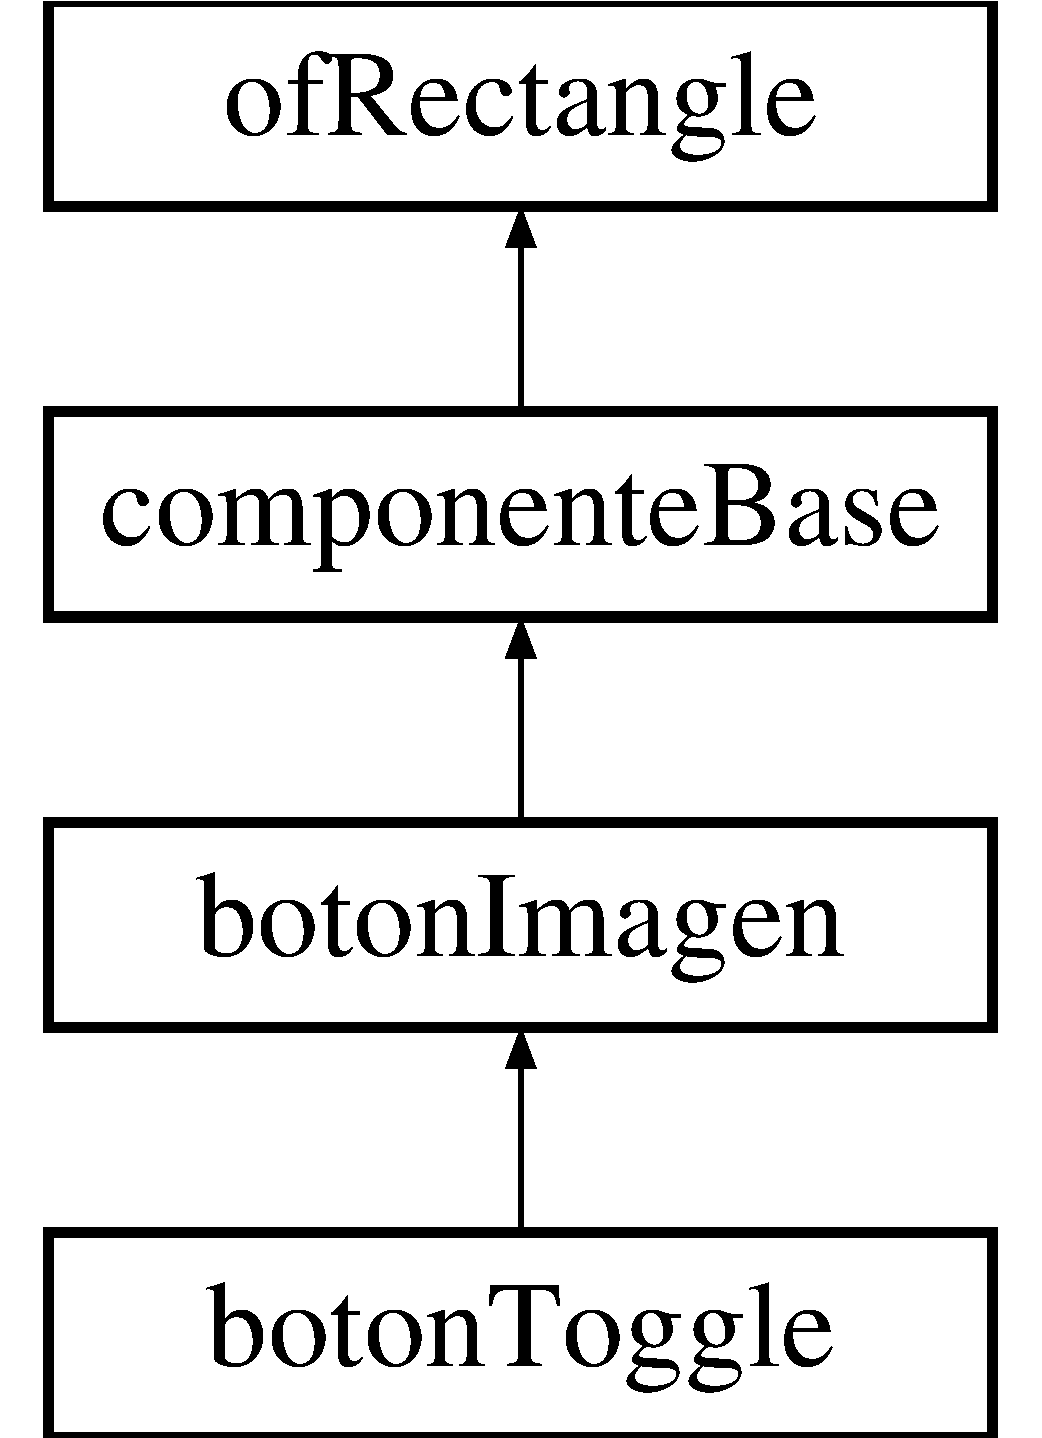
\includegraphics[height=4.000000cm]{classboton_imagen}
\end{center}
\end{figure}
\subsection*{Métodos públicos}
\begin{DoxyCompactItemize}
\item 
\hyperlink{classboton_imagen_a39ee73ee8807ad4339d6a0a080bc8f6d}{boton\+Imagen} (string, float, string, int, of\+Color, int, int, int, int)
\begin{DoxyCompactList}\small\item\em Constructor principal de la clase, define tamaño y posición. \end{DoxyCompactList}\item 
\hyperlink{classboton_imagen_ad6917e2e059fa4a8247ada624663b19a}{boton\+Imagen} (string, float, string, int, of\+Color)
\begin{DoxyCompactList}\small\item\em Constructor secundario de la clase, sin tamaño y posición definidos. \end{DoxyCompactList}\item 
void \hyperlink{classboton_imagen_aca8f9275bf3f03f48d7e34803e0345bf}{set\+Tam} (int, int)
\begin{DoxyCompactList}\small\item\em Asigna tamaño al botón. \end{DoxyCompactList}\item 
void \hyperlink{classboton_imagen_a27a090f89bbf2489401f1e6c5286d3ec}{set\+Pos} (int, int)
\item 
void \hyperlink{classboton_imagen_aa2f66743b229d99cc06b36f5ad16450d}{draw} ()
\begin{DoxyCompactList}\small\item\em Dibuja el componente en pantalla. \end{DoxyCompactList}\end{DoxyCompactItemize}
\subsection*{Atributos protegidos}
\begin{DoxyCompactItemize}
\item 
float \hyperlink{classboton_imagen_a38d03166cf4cc63b616626875fdd817d}{escala}
\begin{DoxyCompactList}\small\item\em Relación de la imagen con respecto al tamaño del botón. \end{DoxyCompactList}\item 
of\+Color \hyperlink{classboton_imagen_ab2d8d1388ec4d76dbcd5e9a61436742c}{color\+Fuente}
\begin{DoxyCompactList}\small\item\em Color del texto. \end{DoxyCompactList}\item 
of\+True\+Type\+Font \hyperlink{classboton_imagen_a7f0f528e711fd891d186b3bfee192e39}{fuente}
\begin{DoxyCompactList}\small\item\em Fuente para dibujar el texto. \end{DoxyCompactList}\item 
string \hyperlink{classboton_imagen_a7118e57f1d4c1d91f2142b908f109f89}{texto}
\begin{DoxyCompactList}\small\item\em Texto que se va a mostrar en la parte interior del botón. \end{DoxyCompactList}\item 
of\+Image \hyperlink{classboton_imagen_a5099abcbecf2cc9d6cdb8cbe5b3a6921}{imagen}
\begin{DoxyCompactList}\small\item\em Imagen que se va a dibujar en el botón. \end{DoxyCompactList}\end{DoxyCompactItemize}
\subsection*{Otros miembros heredados}


\subsection{Descripción detallada}
Botón con imagen y texto. 

Este botón funciona para los entornos que integran pictogramas. Además de tener una imagen el botón puede tener un texto bajo la imagen.

La imagen del botón es escalada para que quepa dentro del botón, tener en consideración que si el botón es cuadrado y la imagen es rectangular se va a perder la proporción de la imagen. Esto es algo que se puede arreglar a la ahora de escalar la imagen en el constructor. 

\subsection{Documentación del constructor y destructor}
\hypertarget{classboton_imagen_a39ee73ee8807ad4339d6a0a080bc8f6d}{}\index{boton\+Imagen@{boton\+Imagen}!boton\+Imagen@{boton\+Imagen}}
\index{boton\+Imagen@{boton\+Imagen}!boton\+Imagen@{boton\+Imagen}}
\subsubsection[{boton\+Imagen(string, float, string, int, of\+Color, int, int, int, int)}]{\setlength{\rightskip}{0pt plus 5cm}boton\+Imagen\+::boton\+Imagen (
\begin{DoxyParamCaption}
\item[{string}]{r, }
\item[{float}]{esc, }
\item[{string}]{t, }
\item[{int}]{tam\+Fuente, }
\item[{of\+Color}]{c, }
\item[{int}]{x, }
\item[{int}]{y, }
\item[{int}]{w, }
\item[{int}]{h}
\end{DoxyParamCaption}
)}\label{classboton_imagen_a39ee73ee8807ad4339d6a0a080bc8f6d}


Constructor principal de la clase, define tamaño y posición. 

Inicializa la fuente y guarda las configuraciones necesarias para dibujarse en pantalla.


\begin{DoxyParams}{Parámetros}
{\em r} & Localizacion de la imagen \\
\hline
{\em esc} & Representa la escala entre la imagen y el tamaño del botón, número real entre 0 y 1 \\
\hline
{\em t} & texto del botón \\
\hline
{\em tam\+Fuente} & tamaño de la fuente del texto \\
\hline
{\em c} & color del texto \\
\hline
{\em x} & localización en el eje x \\
\hline
{\em y} & localización en el eye y \\
\hline
{\em w} & largo del componente \\
\hline
{\em h} & ancho del componente \\
\hline
\end{DoxyParams}
\hypertarget{classboton_imagen_ad6917e2e059fa4a8247ada624663b19a}{}\index{boton\+Imagen@{boton\+Imagen}!boton\+Imagen@{boton\+Imagen}}
\index{boton\+Imagen@{boton\+Imagen}!boton\+Imagen@{boton\+Imagen}}
\subsubsection[{boton\+Imagen(string, float, string, int, of\+Color)}]{\setlength{\rightskip}{0pt plus 5cm}boton\+Imagen\+::boton\+Imagen (
\begin{DoxyParamCaption}
\item[{string}]{r, }
\item[{float}]{esc, }
\item[{string}]{t, }
\item[{int}]{tam\+Fuente, }
\item[{of\+Color}]{c}
\end{DoxyParamCaption}
)}\label{classboton_imagen_ad6917e2e059fa4a8247ada624663b19a}


Constructor secundario de la clase, sin tamaño y posición definidos. 


\begin{DoxyParams}{Parámetros}
{\em r} & Localizacion de la imagen \\
\hline
{\em esc} & Representa la escala entre la imagen y el tamaño del botón, número real entre 0 y 1 \\
\hline
{\em t} & texto del botón \\
\hline
{\em tam\+Fuente} & tamaño de la fuente del texto \\
\hline
{\em c} & color del texto \\
\hline
\end{DoxyParams}


\subsection{Documentación de las funciones miembro}
\hypertarget{classboton_imagen_aa2f66743b229d99cc06b36f5ad16450d}{}\index{boton\+Imagen@{boton\+Imagen}!draw@{draw}}
\index{draw@{draw}!boton\+Imagen@{boton\+Imagen}}
\subsubsection[{draw()}]{\setlength{\rightskip}{0pt plus 5cm}void boton\+Imagen\+::draw (
\begin{DoxyParamCaption}
{}
\end{DoxyParamCaption}
)\hspace{0.3cm}{\ttfamily [virtual]}}\label{classboton_imagen_aa2f66743b229d99cc06b36f5ad16450d}


Dibuja el componente en pantalla. 



Implementa \hyperlink{classcomponente_base_ac6faec0698776f8bfe0e817b9927c0f9}{componente\+Base}.

\hypertarget{classboton_imagen_a27a090f89bbf2489401f1e6c5286d3ec}{}\index{boton\+Imagen@{boton\+Imagen}!set\+Pos@{set\+Pos}}
\index{set\+Pos@{set\+Pos}!boton\+Imagen@{boton\+Imagen}}
\subsubsection[{set\+Pos(int, int)}]{\setlength{\rightskip}{0pt plus 5cm}void boton\+Imagen\+::set\+Pos (
\begin{DoxyParamCaption}
\item[{int}]{x, }
\item[{int}]{y}
\end{DoxyParamCaption}
)}\label{classboton_imagen_a27a090f89bbf2489401f1e6c5286d3ec}

\begin{DoxyParams}{Parámetros}
{\em x} & localización en el eje x \\
\hline
{\em y} & localización en el eye y \\
\hline
\end{DoxyParams}
\hypertarget{classboton_imagen_aca8f9275bf3f03f48d7e34803e0345bf}{}\index{boton\+Imagen@{boton\+Imagen}!set\+Tam@{set\+Tam}}
\index{set\+Tam@{set\+Tam}!boton\+Imagen@{boton\+Imagen}}
\subsubsection[{set\+Tam(int, int)}]{\setlength{\rightskip}{0pt plus 5cm}void boton\+Imagen\+::set\+Tam (
\begin{DoxyParamCaption}
\item[{int}]{w, }
\item[{int}]{h}
\end{DoxyParamCaption}
)}\label{classboton_imagen_aca8f9275bf3f03f48d7e34803e0345bf}


Asigna tamaño al botón. 


\begin{DoxyParams}{Parámetros}
{\em w} & largo del componente \\
\hline
{\em h} & ancho del componente \\
\hline
\end{DoxyParams}


\subsection{Documentación de los datos miembro}
\hypertarget{classboton_imagen_ab2d8d1388ec4d76dbcd5e9a61436742c}{}\index{boton\+Imagen@{boton\+Imagen}!color\+Fuente@{color\+Fuente}}
\index{color\+Fuente@{color\+Fuente}!boton\+Imagen@{boton\+Imagen}}
\subsubsection[{color\+Fuente}]{\setlength{\rightskip}{0pt plus 5cm}of\+Color boton\+Imagen\+::color\+Fuente\hspace{0.3cm}{\ttfamily [protected]}}\label{classboton_imagen_ab2d8d1388ec4d76dbcd5e9a61436742c}


Color del texto. 

\hypertarget{classboton_imagen_a38d03166cf4cc63b616626875fdd817d}{}\index{boton\+Imagen@{boton\+Imagen}!escala@{escala}}
\index{escala@{escala}!boton\+Imagen@{boton\+Imagen}}
\subsubsection[{escala}]{\setlength{\rightskip}{0pt plus 5cm}float boton\+Imagen\+::escala\hspace{0.3cm}{\ttfamily [protected]}}\label{classboton_imagen_a38d03166cf4cc63b616626875fdd817d}


Relación de la imagen con respecto al tamaño del botón. 

\hypertarget{classboton_imagen_a7f0f528e711fd891d186b3bfee192e39}{}\index{boton\+Imagen@{boton\+Imagen}!fuente@{fuente}}
\index{fuente@{fuente}!boton\+Imagen@{boton\+Imagen}}
\subsubsection[{fuente}]{\setlength{\rightskip}{0pt plus 5cm}of\+True\+Type\+Font boton\+Imagen\+::fuente\hspace{0.3cm}{\ttfamily [protected]}}\label{classboton_imagen_a7f0f528e711fd891d186b3bfee192e39}


Fuente para dibujar el texto. 

\hypertarget{classboton_imagen_a5099abcbecf2cc9d6cdb8cbe5b3a6921}{}\index{boton\+Imagen@{boton\+Imagen}!imagen@{imagen}}
\index{imagen@{imagen}!boton\+Imagen@{boton\+Imagen}}
\subsubsection[{imagen}]{\setlength{\rightskip}{0pt plus 5cm}of\+Image boton\+Imagen\+::imagen\hspace{0.3cm}{\ttfamily [protected]}}\label{classboton_imagen_a5099abcbecf2cc9d6cdb8cbe5b3a6921}


Imagen que se va a dibujar en el botón. 

\hypertarget{classboton_imagen_a7118e57f1d4c1d91f2142b908f109f89}{}\index{boton\+Imagen@{boton\+Imagen}!texto@{texto}}
\index{texto@{texto}!boton\+Imagen@{boton\+Imagen}}
\subsubsection[{texto}]{\setlength{\rightskip}{0pt plus 5cm}string boton\+Imagen\+::texto\hspace{0.3cm}{\ttfamily [protected]}}\label{classboton_imagen_a7118e57f1d4c1d91f2142b908f109f89}


Texto que se va a mostrar en la parte interior del botón. 



La documentación para esta clase fue generada a partir de los siguientes ficheros\+:\begin{DoxyCompactItemize}
\item 
C\+:/of\+\_\+v0.\+8.\+4\+\_\+vs\+\_\+release/apps/my\+Apps/\+Robo\+Tracking\+App/src/componentes/\hyperlink{boton_imagen_8h}{boton\+Imagen.\+h}\item 
C\+:/of\+\_\+v0.\+8.\+4\+\_\+vs\+\_\+release/apps/my\+Apps/\+Robo\+Tracking\+App/src/componentes/\hyperlink{boton_imagen_8cpp}{boton\+Imagen.\+cpp}\end{DoxyCompactItemize}

\hypertarget{classboton_simple}{}\section{Referencia de la Clase boton\+Simple}
\label{classboton_simple}\index{boton\+Simple@{boton\+Simple}}


Botón con texto.  




{\ttfamily \#include $<$boton\+Simple.\+h$>$}

Diagrama de herencias de boton\+Simple\begin{figure}[H]
\begin{center}
\leavevmode
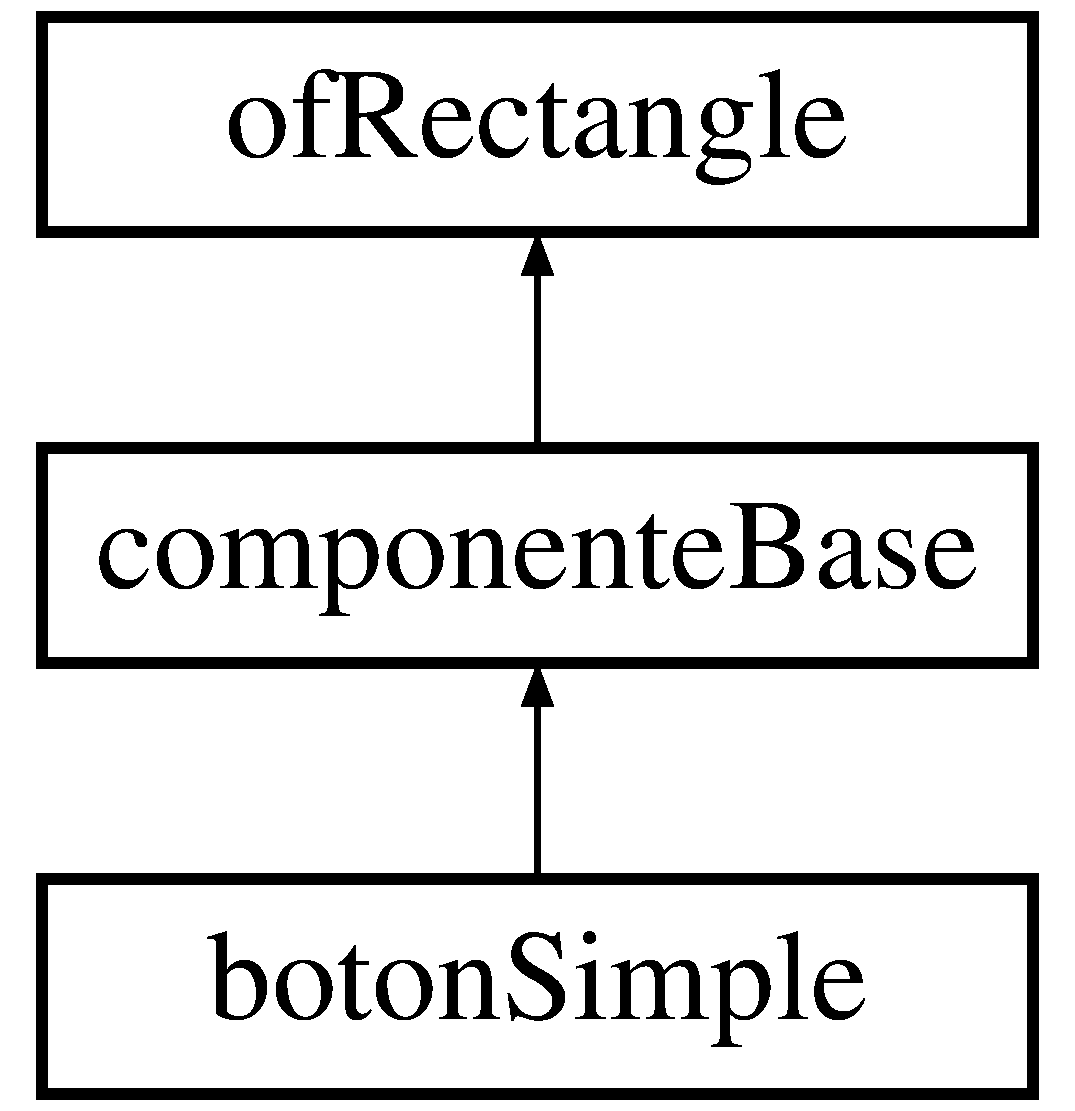
\includegraphics[height=3.000000cm]{classboton_simple}
\end{center}
\end{figure}
\subsection*{Métodos públicos}
\begin{DoxyCompactItemize}
\item 
\hyperlink{classboton_simple_acbcb5c2f8c673c1de738a2282fdca5de}{boton\+Simple} (string, int, of\+Color, int, int, int, int)
\begin{DoxyCompactList}\small\item\em Constructor de la clase. \end{DoxyCompactList}\item 
\hyperlink{classboton_simple_a2d33b48a7757daaf4c26877ec16eba0e}{boton\+Simple} (string, int, of\+Color, int, int, int, int, int)
\item 
void \hyperlink{classboton_simple_a64baaac5439d0ad0d2ec1a11e23a8ad2}{draw} ()
\begin{DoxyCompactList}\small\item\em Dibuja el componente en pantalla. \end{DoxyCompactList}\item 
string \hyperlink{classboton_simple_a57beca159c5aa3ee7055cd3d8f12d2b7}{get\+Texto} ()
\begin{DoxyCompactList}\small\item\em Recupera el texto del botón. \end{DoxyCompactList}\item 
void \hyperlink{classboton_simple_a2e21e1c5c56d5606cc6f63c5f2bf71b7}{set\+Texto} (string)
\begin{DoxyCompactList}\small\item\em Cambia el texto del botón. \end{DoxyCompactList}\end{DoxyCompactItemize}
\subsection*{Atributos privados}
\begin{DoxyCompactItemize}
\item 
of\+Color \hyperlink{classboton_simple_a675afe5f4260c740b013c84dff6e60e1}{color\+Fuente}
\begin{DoxyCompactList}\small\item\em Color de la fuente. \end{DoxyCompactList}\item 
of\+True\+Type\+Font \hyperlink{classboton_simple_aca3777162256e66600ed386b887e4414}{fuente}
\begin{DoxyCompactList}\small\item\em Instancia de la fuente para poder dibujar el texto. \end{DoxyCompactList}\item 
string \hyperlink{classboton_simple_a6093d1fa34187d1f74182f59de6459b9}{texto}
\begin{DoxyCompactList}\small\item\em Contiene el texto del botón. \end{DoxyCompactList}\item 
int \hyperlink{classboton_simple_aa3af0794b6ec6ce74ffb15746bb6fc3c}{alfa}
\end{DoxyCompactItemize}
\subsection*{Otros miembros heredados}


\subsection{Descripción detallada}
Botón con texto. 

Este componente representa un botón con una hilera de caracteres. Se pueden controlar parámetros como el tamaño de la fuente y el color del texto. El texto se dibuja centrado en el componente. 

\subsection{Documentación del constructor y destructor}
\hypertarget{classboton_simple_acbcb5c2f8c673c1de738a2282fdca5de}{}\index{boton\+Simple@{boton\+Simple}!boton\+Simple@{boton\+Simple}}
\index{boton\+Simple@{boton\+Simple}!boton\+Simple@{boton\+Simple}}
\subsubsection[{boton\+Simple(string, int, of\+Color, int, int, int, int)}]{\setlength{\rightskip}{0pt plus 5cm}boton\+Simple\+::boton\+Simple (
\begin{DoxyParamCaption}
\item[{string}]{t, }
\item[{int}]{tam\+Fuente, }
\item[{of\+Color}]{c, }
\item[{int}]{x, }
\item[{int}]{y, }
\item[{int}]{w, }
\item[{int}]{h}
\end{DoxyParamCaption}
)}\label{classboton_simple_acbcb5c2f8c673c1de738a2282fdca5de}


Constructor de la clase. 

Inicializa la fuente y guarda las configuraciones necesarias para dibujarse en pantalla.


\begin{DoxyParams}{Parámetros}
{\em t} & texto del botón \\
\hline
{\em tam\+Fuente} & tamaño de la fuente del texto \\
\hline
{\em c} & color del texto \\
\hline
{\em x} & localización en el eje x \\
\hline
{\em y} & localización en el eye y \\
\hline
{\em w} & largo del componente \\
\hline
{\em h} & ancho del componente \\
\hline
\end{DoxyParams}
\hypertarget{classboton_simple_a2d33b48a7757daaf4c26877ec16eba0e}{}\index{boton\+Simple@{boton\+Simple}!boton\+Simple@{boton\+Simple}}
\index{boton\+Simple@{boton\+Simple}!boton\+Simple@{boton\+Simple}}
\subsubsection[{boton\+Simple(string, int, of\+Color, int, int, int, int, int)}]{\setlength{\rightskip}{0pt plus 5cm}boton\+Simple\+::boton\+Simple (
\begin{DoxyParamCaption}
\item[{string}]{t, }
\item[{int}]{tam\+Fuente, }
\item[{of\+Color}]{c, }
\item[{int}]{x, }
\item[{int}]{y, }
\item[{int}]{w, }
\item[{int}]{h, }
\item[{int}]{a}
\end{DoxyParamCaption}
)}\label{classboton_simple_a2d33b48a7757daaf4c26877ec16eba0e}


\subsection{Documentación de las funciones miembro}
\hypertarget{classboton_simple_a64baaac5439d0ad0d2ec1a11e23a8ad2}{}\index{boton\+Simple@{boton\+Simple}!draw@{draw}}
\index{draw@{draw}!boton\+Simple@{boton\+Simple}}
\subsubsection[{draw()}]{\setlength{\rightskip}{0pt plus 5cm}void boton\+Simple\+::draw (
\begin{DoxyParamCaption}
{}
\end{DoxyParamCaption}
)\hspace{0.3cm}{\ttfamily [virtual]}}\label{classboton_simple_a64baaac5439d0ad0d2ec1a11e23a8ad2}


Dibuja el componente en pantalla. 



Implementa \hyperlink{classcomponente_base_ac6faec0698776f8bfe0e817b9927c0f9}{componente\+Base}.

\hypertarget{classboton_simple_a57beca159c5aa3ee7055cd3d8f12d2b7}{}\index{boton\+Simple@{boton\+Simple}!get\+Texto@{get\+Texto}}
\index{get\+Texto@{get\+Texto}!boton\+Simple@{boton\+Simple}}
\subsubsection[{get\+Texto()}]{\setlength{\rightskip}{0pt plus 5cm}string boton\+Simple\+::get\+Texto (
\begin{DoxyParamCaption}
{}
\end{DoxyParamCaption}
)}\label{classboton_simple_a57beca159c5aa3ee7055cd3d8f12d2b7}


Recupera el texto del botón. 

\hypertarget{classboton_simple_a2e21e1c5c56d5606cc6f63c5f2bf71b7}{}\index{boton\+Simple@{boton\+Simple}!set\+Texto@{set\+Texto}}
\index{set\+Texto@{set\+Texto}!boton\+Simple@{boton\+Simple}}
\subsubsection[{set\+Texto(string)}]{\setlength{\rightskip}{0pt plus 5cm}void boton\+Simple\+::set\+Texto (
\begin{DoxyParamCaption}
\item[{string}]{t}
\end{DoxyParamCaption}
)}\label{classboton_simple_a2e21e1c5c56d5606cc6f63c5f2bf71b7}


Cambia el texto del botón. 



\subsection{Documentación de los datos miembro}
\hypertarget{classboton_simple_aa3af0794b6ec6ce74ffb15746bb6fc3c}{}\index{boton\+Simple@{boton\+Simple}!alfa@{alfa}}
\index{alfa@{alfa}!boton\+Simple@{boton\+Simple}}
\subsubsection[{alfa}]{\setlength{\rightskip}{0pt plus 5cm}int boton\+Simple\+::alfa\hspace{0.3cm}{\ttfamily [private]}}\label{classboton_simple_aa3af0794b6ec6ce74ffb15746bb6fc3c}
\hypertarget{classboton_simple_a675afe5f4260c740b013c84dff6e60e1}{}\index{boton\+Simple@{boton\+Simple}!color\+Fuente@{color\+Fuente}}
\index{color\+Fuente@{color\+Fuente}!boton\+Simple@{boton\+Simple}}
\subsubsection[{color\+Fuente}]{\setlength{\rightskip}{0pt plus 5cm}of\+Color boton\+Simple\+::color\+Fuente\hspace{0.3cm}{\ttfamily [private]}}\label{classboton_simple_a675afe5f4260c740b013c84dff6e60e1}


Color de la fuente. 

\hypertarget{classboton_simple_aca3777162256e66600ed386b887e4414}{}\index{boton\+Simple@{boton\+Simple}!fuente@{fuente}}
\index{fuente@{fuente}!boton\+Simple@{boton\+Simple}}
\subsubsection[{fuente}]{\setlength{\rightskip}{0pt plus 5cm}of\+True\+Type\+Font boton\+Simple\+::fuente\hspace{0.3cm}{\ttfamily [private]}}\label{classboton_simple_aca3777162256e66600ed386b887e4414}


Instancia de la fuente para poder dibujar el texto. 

\hypertarget{classboton_simple_a6093d1fa34187d1f74182f59de6459b9}{}\index{boton\+Simple@{boton\+Simple}!texto@{texto}}
\index{texto@{texto}!boton\+Simple@{boton\+Simple}}
\subsubsection[{texto}]{\setlength{\rightskip}{0pt plus 5cm}string boton\+Simple\+::texto\hspace{0.3cm}{\ttfamily [private]}}\label{classboton_simple_a6093d1fa34187d1f74182f59de6459b9}


Contiene el texto del botón. 



La documentación para esta clase fue generada a partir de los siguientes ficheros\+:\begin{DoxyCompactItemize}
\item 
C\+:/of\+\_\+v0.\+8.\+4\+\_\+vs\+\_\+release/apps/my\+Apps/\+Robo\+Tracking\+App/src/componentes/\hyperlink{boton_simple_8h}{boton\+Simple.\+h}\item 
C\+:/of\+\_\+v0.\+8.\+4\+\_\+vs\+\_\+release/apps/my\+Apps/\+Robo\+Tracking\+App/src/componentes/\hyperlink{boton_simple_8cpp}{boton\+Simple.\+cpp}\end{DoxyCompactItemize}

\hypertarget{classboton_toggle}{}\section{Referencia de la Clase boton\+Toggle}
\label{classboton_toggle}\index{boton\+Toggle@{boton\+Toggle}}


Botón que alterna dos imagenes y textos.  




{\ttfamily \#include $<$boton\+Toggle.\+h$>$}

Diagrama de herencias de boton\+Toggle\begin{figure}[H]
\begin{center}
\leavevmode
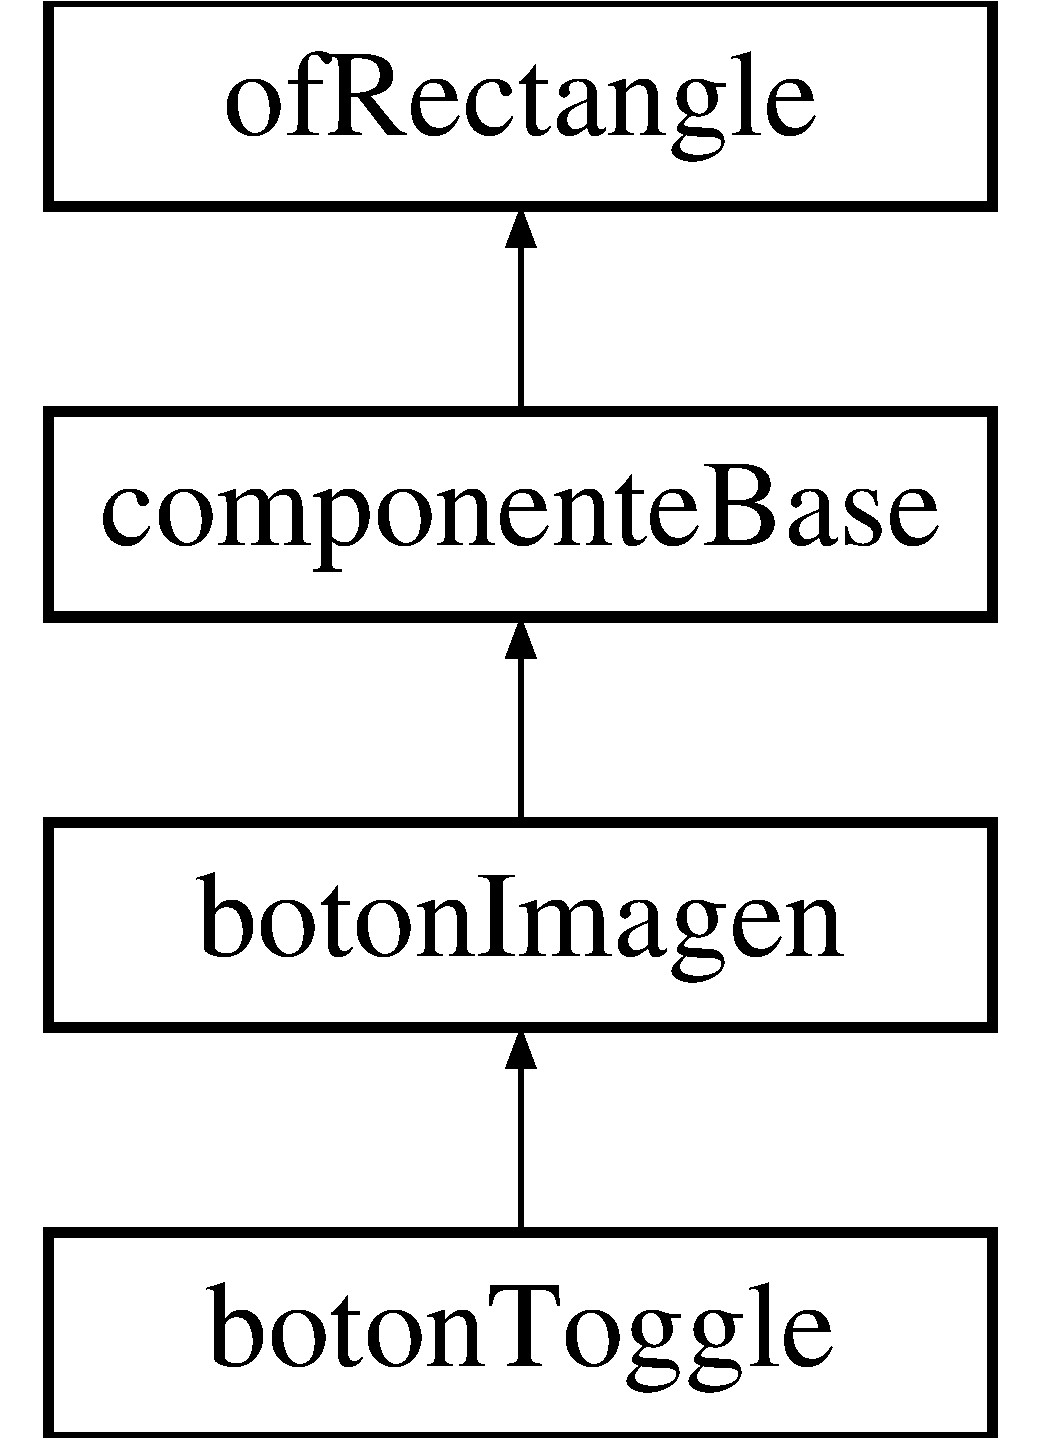
\includegraphics[height=4.000000cm]{classboton_toggle}
\end{center}
\end{figure}
\subsection*{Métodos públicos}
\begin{DoxyCompactItemize}
\item 
\hyperlink{classboton_toggle_a53ca0ae03d7125318e8b88993f8ed936}{boton\+Toggle} (string, string, float, string, string, int, of\+Color, int, int, int, int)
\begin{DoxyCompactList}\small\item\em Constructor principal de la clase, define tamaño y posición. \end{DoxyCompactList}\item 
\hyperlink{classboton_toggle_ad193dda2df6e4399a3171a2d5ecc612f}{boton\+Toggle} (string, string, float, string, string, int, of\+Color)
\begin{DoxyCompactList}\small\item\em Constructor secundario de la clase, sin tamaño y posición definidos. \end{DoxyCompactList}\item 
bool \hyperlink{classboton_toggle_a067fa2bd02fd019d5c6c062ec8d521c0}{update} (float, float, float, float, bool)
\begin{DoxyCompactList}\small\item\em Implementa el cambio de imagen y texto si el usuario hizo clic. \end{DoxyCompactList}\item 
bool \hyperlink{classboton_toggle_a6da75216bda1e716f10cb1baec792cd0}{state} ()
\begin{DoxyCompactList}\small\item\em Devuelve el estado del botón. \end{DoxyCompactList}\item 
void \hyperlink{classboton_toggle_a5a24ccd035199173e96b36a9dec4927f}{toggle} ()
\begin{DoxyCompactList}\small\item\em Cambia el estado del botón. \end{DoxyCompactList}\end{DoxyCompactItemize}
\subsection*{Atributos privados}
\begin{DoxyCompactItemize}
\item 
bool \hyperlink{classboton_toggle_a16e1fc2e8c6b3bfc76f1de28f9623740}{toggle\+State}
\begin{DoxyCompactList}\small\item\em Define el estado del botón, se inicializa en false. \end{DoxyCompactList}\item 
string \hyperlink{classboton_toggle_acd9a4699cc7fcb3facda61450bafa25f}{ruta1}
\begin{DoxyCompactList}\small\item\em Localización de la imagen del estado 1. \end{DoxyCompactList}\item 
string \hyperlink{classboton_toggle_a29e4c1705e45c20f62a77176b7b2ae2d}{ruta2}
\begin{DoxyCompactList}\small\item\em Localización de la imagen del estado 2. \end{DoxyCompactList}\item 
string \hyperlink{classboton_toggle_abd3f33fb266429ad6697518506bedce8}{texto1}
\begin{DoxyCompactList}\small\item\em Texto del estado 1. \end{DoxyCompactList}\item 
string \hyperlink{classboton_toggle_a838680f64548815ecac688f7bd3cb59c}{texto2}
\begin{DoxyCompactList}\small\item\em Texto del estado 2. \end{DoxyCompactList}\item 
float \hyperlink{classboton_toggle_aec530290e05f262e49cd41ea80914bfb}{escala}
\begin{DoxyCompactList}\small\item\em Escalas de las imagenes. \end{DoxyCompactList}\item 
int \hyperlink{classboton_toggle_aa76dc9adf8e8b4513bf839a061ce2129}{w}
\begin{DoxyCompactList}\small\item\em Largo del botón. \end{DoxyCompactList}\item 
int \hyperlink{classboton_toggle_a1e88ceaf2b11a3f376f1bed5751bcbe2}{h}
\begin{DoxyCompactList}\small\item\em Ancho del botón. \end{DoxyCompactList}\end{DoxyCompactItemize}
\subsection*{Otros miembros heredados}


\subsection{Descripción detallada}
Botón que alterna dos imagenes y textos. 

Este botón implementa la funcionalidad de alternar estados. Se definen dos pares de imagenes y textos. 

\subsection{Documentación del constructor y destructor}
\hypertarget{classboton_toggle_a53ca0ae03d7125318e8b88993f8ed936}{}\index{boton\+Toggle@{boton\+Toggle}!boton\+Toggle@{boton\+Toggle}}
\index{boton\+Toggle@{boton\+Toggle}!boton\+Toggle@{boton\+Toggle}}
\subsubsection[{boton\+Toggle(string, string, float, string, string, int, of\+Color, int, int, int, int)}]{\setlength{\rightskip}{0pt plus 5cm}boton\+Toggle\+::boton\+Toggle (
\begin{DoxyParamCaption}
\item[{string}]{r1, }
\item[{string}]{r2, }
\item[{float}]{esc, }
\item[{string}]{t1, }
\item[{string}]{t2, }
\item[{int}]{tam\+Fuente, }
\item[{of\+Color}]{c, }
\item[{int}]{x, }
\item[{int}]{y, }
\item[{int}]{w\+\_\+, }
\item[{int}]{h\+\_\+}
\end{DoxyParamCaption}
)}\label{classboton_toggle_a53ca0ae03d7125318e8b88993f8ed936}


Constructor principal de la clase, define tamaño y posición. 

Inicializa la fuente y guarda las configuraciones necesarias para dibujarse en pantalla.


\begin{DoxyParams}{Parámetros}
{\em r1} & Localizacion de la imagen 1 \\
\hline
{\em r2} & Localizacion de la imagen 2 \\
\hline
{\em esc} & Representa la escala entre la imagen y el tamaño del botón, número real entre 0 y 1 \\
\hline
{\em t1} & texto 1 del botón \\
\hline
{\em t2} & texto 2 del botón \\
\hline
{\em tam\+Fuente} & tamaño de la fuente del texto \\
\hline
{\em c} & color del texto \\
\hline
{\em x} & localización en el eje x \\
\hline
{\em y} & localización en el eye y \\
\hline
{\em w\+\_\+} & largo del componente \\
\hline
{\em h\+\_\+} & ancho del componente \\
\hline
\end{DoxyParams}
\hypertarget{classboton_toggle_ad193dda2df6e4399a3171a2d5ecc612f}{}\index{boton\+Toggle@{boton\+Toggle}!boton\+Toggle@{boton\+Toggle}}
\index{boton\+Toggle@{boton\+Toggle}!boton\+Toggle@{boton\+Toggle}}
\subsubsection[{boton\+Toggle(string, string, float, string, string, int, of\+Color)}]{\setlength{\rightskip}{0pt plus 5cm}boton\+Toggle\+::boton\+Toggle (
\begin{DoxyParamCaption}
\item[{string}]{r1, }
\item[{string}]{r2, }
\item[{float}]{esc, }
\item[{string}]{t1, }
\item[{string}]{t2, }
\item[{int}]{tam\+Fuente, }
\item[{of\+Color}]{c}
\end{DoxyParamCaption}
)}\label{classboton_toggle_ad193dda2df6e4399a3171a2d5ecc612f}


Constructor secundario de la clase, sin tamaño y posición definidos. 


\begin{DoxyParams}{Parámetros}
{\em r1} & Localizacion de la imagen 1 \\
\hline
{\em r2} & Localizacion de la imagen 2 \\
\hline
{\em esc} & Representa la escala entre la imagen y el tamaño del botón, número real entre 0 y 1 \\
\hline
{\em t1} & texto 1 del botón \\
\hline
{\em t2} & texto 2 del botón \\
\hline
{\em tam\+Fuente} & tamaño de la fuente del texto \\
\hline
{\em c} & color del texto \\
\hline
\end{DoxyParams}


\subsection{Documentación de las funciones miembro}
\hypertarget{classboton_toggle_a6da75216bda1e716f10cb1baec792cd0}{}\index{boton\+Toggle@{boton\+Toggle}!state@{state}}
\index{state@{state}!boton\+Toggle@{boton\+Toggle}}
\subsubsection[{state()}]{\setlength{\rightskip}{0pt plus 5cm}bool boton\+Toggle\+::state (
\begin{DoxyParamCaption}
{}
\end{DoxyParamCaption}
)}\label{classboton_toggle_a6da75216bda1e716f10cb1baec792cd0}


Devuelve el estado del botón. 

\begin{DoxyReturn}{Devuelve}
true si el botón está en el estado 2 
\end{DoxyReturn}
\hypertarget{classboton_toggle_a5a24ccd035199173e96b36a9dec4927f}{}\index{boton\+Toggle@{boton\+Toggle}!toggle@{toggle}}
\index{toggle@{toggle}!boton\+Toggle@{boton\+Toggle}}
\subsubsection[{toggle()}]{\setlength{\rightskip}{0pt plus 5cm}void boton\+Toggle\+::toggle (
\begin{DoxyParamCaption}
{}
\end{DoxyParamCaption}
)}\label{classboton_toggle_a5a24ccd035199173e96b36a9dec4927f}


Cambia el estado del botón. 

\hypertarget{classboton_toggle_a067fa2bd02fd019d5c6c062ec8d521c0}{}\index{boton\+Toggle@{boton\+Toggle}!update@{update}}
\index{update@{update}!boton\+Toggle@{boton\+Toggle}}
\subsubsection[{update(float, float, float, float, bool)}]{\setlength{\rightskip}{0pt plus 5cm}bool boton\+Toggle\+::update (
\begin{DoxyParamCaption}
\item[{float}]{x\+M, }
\item[{float}]{y\+M, }
\item[{float}]{x\+L, }
\item[{float}]{y\+L, }
\item[{bool}]{c}
\end{DoxyParamCaption}
)}\label{classboton_toggle_a067fa2bd02fd019d5c6c062ec8d521c0}


Implementa el cambio de imagen y texto si el usuario hizo clic. 


\begin{DoxyParams}{Parámetros}
{\em x\+M} & coordenada x de la entrada visual \\
\hline
{\em y\+M} & coordenada y de la entrada visual \\
\hline
{\em x\+L} & coordenada x del componente de gestos \\
\hline
{\em y\+L} & coordenada y del componente de gestos \\
\hline
{\em c} & indica si el usuario ha hecho el gesto para el clic\\
\hline
\end{DoxyParams}
\begin{DoxyReturn}{Devuelve}
true si el usuario hizo clic sobre el componente 
\end{DoxyReturn}


\subsection{Documentación de los datos miembro}
\hypertarget{classboton_toggle_aec530290e05f262e49cd41ea80914bfb}{}\index{boton\+Toggle@{boton\+Toggle}!escala@{escala}}
\index{escala@{escala}!boton\+Toggle@{boton\+Toggle}}
\subsubsection[{escala}]{\setlength{\rightskip}{0pt plus 5cm}float boton\+Toggle\+::escala\hspace{0.3cm}{\ttfamily [private]}}\label{classboton_toggle_aec530290e05f262e49cd41ea80914bfb}


Escalas de las imagenes. 

\hypertarget{classboton_toggle_a1e88ceaf2b11a3f376f1bed5751bcbe2}{}\index{boton\+Toggle@{boton\+Toggle}!h@{h}}
\index{h@{h}!boton\+Toggle@{boton\+Toggle}}
\subsubsection[{h}]{\setlength{\rightskip}{0pt plus 5cm}int boton\+Toggle\+::h\hspace{0.3cm}{\ttfamily [private]}}\label{classboton_toggle_a1e88ceaf2b11a3f376f1bed5751bcbe2}


Ancho del botón. 

\hypertarget{classboton_toggle_acd9a4699cc7fcb3facda61450bafa25f}{}\index{boton\+Toggle@{boton\+Toggle}!ruta1@{ruta1}}
\index{ruta1@{ruta1}!boton\+Toggle@{boton\+Toggle}}
\subsubsection[{ruta1}]{\setlength{\rightskip}{0pt plus 5cm}string boton\+Toggle\+::ruta1\hspace{0.3cm}{\ttfamily [private]}}\label{classboton_toggle_acd9a4699cc7fcb3facda61450bafa25f}


Localización de la imagen del estado 1. 

\hypertarget{classboton_toggle_a29e4c1705e45c20f62a77176b7b2ae2d}{}\index{boton\+Toggle@{boton\+Toggle}!ruta2@{ruta2}}
\index{ruta2@{ruta2}!boton\+Toggle@{boton\+Toggle}}
\subsubsection[{ruta2}]{\setlength{\rightskip}{0pt plus 5cm}string boton\+Toggle\+::ruta2\hspace{0.3cm}{\ttfamily [private]}}\label{classboton_toggle_a29e4c1705e45c20f62a77176b7b2ae2d}


Localización de la imagen del estado 2. 

\hypertarget{classboton_toggle_abd3f33fb266429ad6697518506bedce8}{}\index{boton\+Toggle@{boton\+Toggle}!texto1@{texto1}}
\index{texto1@{texto1}!boton\+Toggle@{boton\+Toggle}}
\subsubsection[{texto1}]{\setlength{\rightskip}{0pt plus 5cm}string boton\+Toggle\+::texto1\hspace{0.3cm}{\ttfamily [private]}}\label{classboton_toggle_abd3f33fb266429ad6697518506bedce8}


Texto del estado 1. 

\hypertarget{classboton_toggle_a838680f64548815ecac688f7bd3cb59c}{}\index{boton\+Toggle@{boton\+Toggle}!texto2@{texto2}}
\index{texto2@{texto2}!boton\+Toggle@{boton\+Toggle}}
\subsubsection[{texto2}]{\setlength{\rightskip}{0pt plus 5cm}string boton\+Toggle\+::texto2\hspace{0.3cm}{\ttfamily [private]}}\label{classboton_toggle_a838680f64548815ecac688f7bd3cb59c}


Texto del estado 2. 

\hypertarget{classboton_toggle_a16e1fc2e8c6b3bfc76f1de28f9623740}{}\index{boton\+Toggle@{boton\+Toggle}!toggle\+State@{toggle\+State}}
\index{toggle\+State@{toggle\+State}!boton\+Toggle@{boton\+Toggle}}
\subsubsection[{toggle\+State}]{\setlength{\rightskip}{0pt plus 5cm}bool boton\+Toggle\+::toggle\+State\hspace{0.3cm}{\ttfamily [private]}}\label{classboton_toggle_a16e1fc2e8c6b3bfc76f1de28f9623740}


Define el estado del botón, se inicializa en false. 

\hypertarget{classboton_toggle_aa76dc9adf8e8b4513bf839a061ce2129}{}\index{boton\+Toggle@{boton\+Toggle}!w@{w}}
\index{w@{w}!boton\+Toggle@{boton\+Toggle}}
\subsubsection[{w}]{\setlength{\rightskip}{0pt plus 5cm}int boton\+Toggle\+::w\hspace{0.3cm}{\ttfamily [private]}}\label{classboton_toggle_aa76dc9adf8e8b4513bf839a061ce2129}


Largo del botón. 



La documentación para esta clase fue generada a partir de los siguientes ficheros\+:\begin{DoxyCompactItemize}
\item 
C\+:/of\+\_\+v0.\+8.\+4\+\_\+vs\+\_\+release/apps/my\+Apps/\+Robo\+Tracking\+App/src/componentes/\hyperlink{boton_toggle_8h}{boton\+Toggle.\+h}\item 
C\+:/of\+\_\+v0.\+8.\+4\+\_\+vs\+\_\+release/apps/my\+Apps/\+Robo\+Tracking\+App/src/componentes/\hyperlink{boton_toggle_8cpp}{boton\+Toggle.\+cpp}\end{DoxyCompactItemize}

\hypertarget{classcaja_texto}{}\section{Referencia de la Clase caja\+Texto}
\label{classcaja_texto}\index{caja\+Texto@{caja\+Texto}}


Caja para mostrar texto.  




{\ttfamily \#include $<$caja\+Texto.\+h$>$}

Diagrama de herencias de caja\+Texto\begin{figure}[H]
\begin{center}
\leavevmode
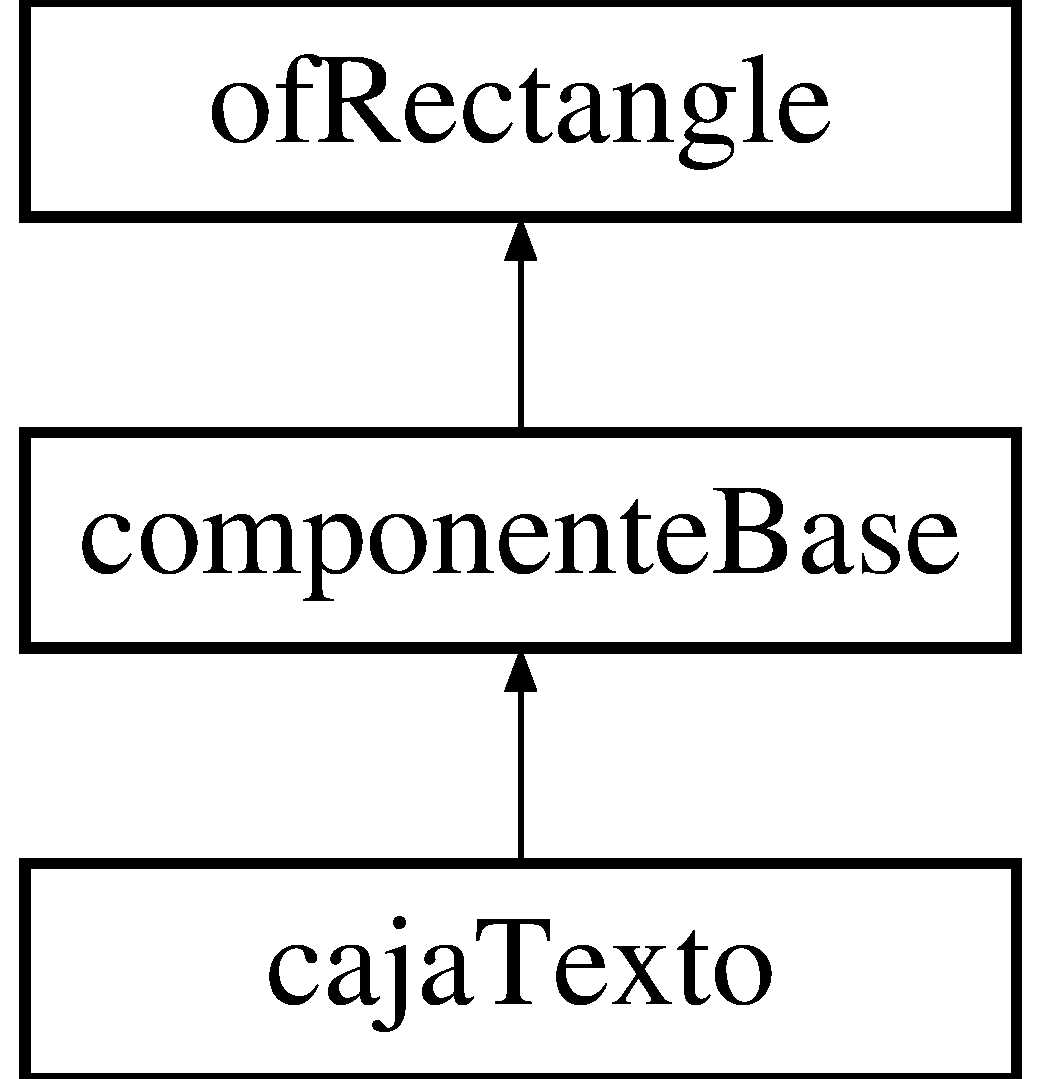
\includegraphics[height=3.000000cm]{classcaja_texto}
\end{center}
\end{figure}
\subsection*{Métodos públicos}
\begin{DoxyCompactItemize}
\item 
\hyperlink{classcaja_texto_aee455629d334f28613f43b6a61d16f14}{caja\+Texto} (int, of\+Color, int, int, int, int)
\begin{DoxyCompactList}\small\item\em Constructor de la clase. \end{DoxyCompactList}\item 
\hyperlink{classcaja_texto_a66c1f439ba50e8df9a13eb5a53085c52}{caja\+Texto} (int, of\+Color, int, int, int, int, int)
\item 
void \hyperlink{classcaja_texto_a5bc02d7f55e12fd32715e4509853a558}{draw} ()
\begin{DoxyCompactList}\small\item\em Dibuja el componente en pantalla. \end{DoxyCompactList}\item 
void \hyperlink{classcaja_texto_ae6326da3ec5842eb0ff41208d22b1567}{append\+Texto} (string)
\begin{DoxyCompactList}\small\item\em Agrega texto al final de la hilera actual. \end{DoxyCompactList}\item 
void \hyperlink{classcaja_texto_ab9362a01f444db0bed5032b9ec585905}{borrar\+Caracter} ()
\begin{DoxyCompactList}\small\item\em Borra el último caracter del texto. \end{DoxyCompactList}\item 
string \hyperlink{classcaja_texto_ab5e4ed49e9aaa7176e9186b085a07621}{get\+Texto} ()
\begin{DoxyCompactList}\small\item\em Devuelve el texto actual. \end{DoxyCompactList}\item 
void \hyperlink{classcaja_texto_a088cc70dc707de2cf00bed4f906521c0}{limpiar} ()
\end{DoxyCompactItemize}
\subsection*{Atributos privados}
\begin{DoxyCompactItemize}
\item 
of\+Color \hyperlink{classcaja_texto_a281b136399f6b3ee3fedfaa9069bebad}{color\+Fuente}
\begin{DoxyCompactList}\small\item\em Color del texto. \end{DoxyCompactList}\item 
of\+True\+Type\+Font \hyperlink{classcaja_texto_aa5cbc731d2fc56d87210d6ae6d2319b0}{fuente}
\begin{DoxyCompactList}\small\item\em Fuente del texto. \end{DoxyCompactList}\item 
string \hyperlink{classcaja_texto_a5b62049df6eb5efb5831b57b4958d115}{texto}
\begin{DoxyCompactList}\small\item\em Texto que se está mostrando en la caja. \end{DoxyCompactList}\item 
int \hyperlink{classcaja_texto_a779378b7d6c746df32e86b0f3a7eaa0e}{margen\+Max\+Texto}
\item 
int \hyperlink{classcaja_texto_a1003061aaaac05741ede0303e5a7f6cc}{margen\+Min\+Texto}
\item 
int \hyperlink{classcaja_texto_a621c5f95927c538ca286827a06d861d0}{fuente\+Inicial}
\item 
int \hyperlink{classcaja_texto_ab5e905a37e7247d0f2b0c139ad49970e}{razon\+Cambio\+Fuente}
\item 
int \hyperlink{classcaja_texto_aa52a0f1d3f9041daa3f0e270214d85aa}{alfa}
\item 
of\+Color \hyperlink{classcaja_texto_a7c9fcc0013453675b9c08c4db98ee615}{color}
\end{DoxyCompactItemize}
\subsection*{Otros miembros heredados}


\subsection{Descripción detallada}
Caja para mostrar texto. 

El texto está centrado y pensado para mostrar máximo una oración, el soporte para párrafos y barras de scroll no están implementados 

\subsection{Documentación del constructor y destructor}
\hypertarget{classcaja_texto_aee455629d334f28613f43b6a61d16f14}{}\index{caja\+Texto@{caja\+Texto}!caja\+Texto@{caja\+Texto}}
\index{caja\+Texto@{caja\+Texto}!caja\+Texto@{caja\+Texto}}
\subsubsection[{caja\+Texto(int, of\+Color, int, int, int, int)}]{\setlength{\rightskip}{0pt plus 5cm}caja\+Texto\+::caja\+Texto (
\begin{DoxyParamCaption}
\item[{int}]{tam\+Fuente, }
\item[{of\+Color}]{c, }
\item[{int}]{x, }
\item[{int}]{y, }
\item[{int}]{w, }
\item[{int}]{h}
\end{DoxyParamCaption}
)}\label{classcaja_texto_aee455629d334f28613f43b6a61d16f14}


Constructor de la clase. 

Inicializa la fuente y guarda las configuraciones necesarias para dibujarse en pantalla. \begin{DoxyVerb}\param tamFuente tamaño de la fuente del texto
\param c color del texto
\param x localización en el eje x
\param y localización en el eye y
\param w largo del componente
\param h ancho del componente\end{DoxyVerb}
 \hypertarget{classcaja_texto_a66c1f439ba50e8df9a13eb5a53085c52}{}\index{caja\+Texto@{caja\+Texto}!caja\+Texto@{caja\+Texto}}
\index{caja\+Texto@{caja\+Texto}!caja\+Texto@{caja\+Texto}}
\subsubsection[{caja\+Texto(int, of\+Color, int, int, int, int, int)}]{\setlength{\rightskip}{0pt plus 5cm}caja\+Texto\+::caja\+Texto (
\begin{DoxyParamCaption}
\item[{int}]{tam\+Fuente, }
\item[{of\+Color}]{c, }
\item[{int}]{x, }
\item[{int}]{y, }
\item[{int}]{w, }
\item[{int}]{h, }
\item[{int}]{a}
\end{DoxyParamCaption}
)}\label{classcaja_texto_a66c1f439ba50e8df9a13eb5a53085c52}


\subsection{Documentación de las funciones miembro}
\hypertarget{classcaja_texto_ae6326da3ec5842eb0ff41208d22b1567}{}\index{caja\+Texto@{caja\+Texto}!append\+Texto@{append\+Texto}}
\index{append\+Texto@{append\+Texto}!caja\+Texto@{caja\+Texto}}
\subsubsection[{append\+Texto(string)}]{\setlength{\rightskip}{0pt plus 5cm}void caja\+Texto\+::append\+Texto (
\begin{DoxyParamCaption}
\item[{string}]{t}
\end{DoxyParamCaption}
)}\label{classcaja_texto_ae6326da3ec5842eb0ff41208d22b1567}


Agrega texto al final de la hilera actual. 

\hypertarget{classcaja_texto_ab9362a01f444db0bed5032b9ec585905}{}\index{caja\+Texto@{caja\+Texto}!borrar\+Caracter@{borrar\+Caracter}}
\index{borrar\+Caracter@{borrar\+Caracter}!caja\+Texto@{caja\+Texto}}
\subsubsection[{borrar\+Caracter()}]{\setlength{\rightskip}{0pt plus 5cm}void caja\+Texto\+::borrar\+Caracter (
\begin{DoxyParamCaption}
{}
\end{DoxyParamCaption}
)}\label{classcaja_texto_ab9362a01f444db0bed5032b9ec585905}


Borra el último caracter del texto. 

\hypertarget{classcaja_texto_a5bc02d7f55e12fd32715e4509853a558}{}\index{caja\+Texto@{caja\+Texto}!draw@{draw}}
\index{draw@{draw}!caja\+Texto@{caja\+Texto}}
\subsubsection[{draw()}]{\setlength{\rightskip}{0pt plus 5cm}void caja\+Texto\+::draw (
\begin{DoxyParamCaption}
{}
\end{DoxyParamCaption}
)\hspace{0.3cm}{\ttfamily [virtual]}}\label{classcaja_texto_a5bc02d7f55e12fd32715e4509853a558}


Dibuja el componente en pantalla. 



Implementa \hyperlink{classcomponente_base_ac6faec0698776f8bfe0e817b9927c0f9}{componente\+Base}.

\hypertarget{classcaja_texto_ab5e4ed49e9aaa7176e9186b085a07621}{}\index{caja\+Texto@{caja\+Texto}!get\+Texto@{get\+Texto}}
\index{get\+Texto@{get\+Texto}!caja\+Texto@{caja\+Texto}}
\subsubsection[{get\+Texto()}]{\setlength{\rightskip}{0pt plus 5cm}string caja\+Texto\+::get\+Texto (
\begin{DoxyParamCaption}
{}
\end{DoxyParamCaption}
)}\label{classcaja_texto_ab5e4ed49e9aaa7176e9186b085a07621}


Devuelve el texto actual. 

\hypertarget{classcaja_texto_a088cc70dc707de2cf00bed4f906521c0}{}\index{caja\+Texto@{caja\+Texto}!limpiar@{limpiar}}
\index{limpiar@{limpiar}!caja\+Texto@{caja\+Texto}}
\subsubsection[{limpiar()}]{\setlength{\rightskip}{0pt plus 5cm}void caja\+Texto\+::limpiar (
\begin{DoxyParamCaption}
{}
\end{DoxyParamCaption}
)}\label{classcaja_texto_a088cc70dc707de2cf00bed4f906521c0}


\subsection{Documentación de los datos miembro}
\hypertarget{classcaja_texto_aa52a0f1d3f9041daa3f0e270214d85aa}{}\index{caja\+Texto@{caja\+Texto}!alfa@{alfa}}
\index{alfa@{alfa}!caja\+Texto@{caja\+Texto}}
\subsubsection[{alfa}]{\setlength{\rightskip}{0pt plus 5cm}int caja\+Texto\+::alfa\hspace{0.3cm}{\ttfamily [private]}}\label{classcaja_texto_aa52a0f1d3f9041daa3f0e270214d85aa}
\hypertarget{classcaja_texto_a7c9fcc0013453675b9c08c4db98ee615}{}\index{caja\+Texto@{caja\+Texto}!color@{color}}
\index{color@{color}!caja\+Texto@{caja\+Texto}}
\subsubsection[{color}]{\setlength{\rightskip}{0pt plus 5cm}of\+Color caja\+Texto\+::color\hspace{0.3cm}{\ttfamily [private]}}\label{classcaja_texto_a7c9fcc0013453675b9c08c4db98ee615}
\hypertarget{classcaja_texto_a281b136399f6b3ee3fedfaa9069bebad}{}\index{caja\+Texto@{caja\+Texto}!color\+Fuente@{color\+Fuente}}
\index{color\+Fuente@{color\+Fuente}!caja\+Texto@{caja\+Texto}}
\subsubsection[{color\+Fuente}]{\setlength{\rightskip}{0pt plus 5cm}of\+Color caja\+Texto\+::color\+Fuente\hspace{0.3cm}{\ttfamily [private]}}\label{classcaja_texto_a281b136399f6b3ee3fedfaa9069bebad}


Color del texto. 

\hypertarget{classcaja_texto_aa5cbc731d2fc56d87210d6ae6d2319b0}{}\index{caja\+Texto@{caja\+Texto}!fuente@{fuente}}
\index{fuente@{fuente}!caja\+Texto@{caja\+Texto}}
\subsubsection[{fuente}]{\setlength{\rightskip}{0pt plus 5cm}of\+True\+Type\+Font caja\+Texto\+::fuente\hspace{0.3cm}{\ttfamily [private]}}\label{classcaja_texto_aa5cbc731d2fc56d87210d6ae6d2319b0}


Fuente del texto. 

\hypertarget{classcaja_texto_a621c5f95927c538ca286827a06d861d0}{}\index{caja\+Texto@{caja\+Texto}!fuente\+Inicial@{fuente\+Inicial}}
\index{fuente\+Inicial@{fuente\+Inicial}!caja\+Texto@{caja\+Texto}}
\subsubsection[{fuente\+Inicial}]{\setlength{\rightskip}{0pt plus 5cm}int caja\+Texto\+::fuente\+Inicial\hspace{0.3cm}{\ttfamily [private]}}\label{classcaja_texto_a621c5f95927c538ca286827a06d861d0}
\hypertarget{classcaja_texto_a779378b7d6c746df32e86b0f3a7eaa0e}{}\index{caja\+Texto@{caja\+Texto}!margen\+Max\+Texto@{margen\+Max\+Texto}}
\index{margen\+Max\+Texto@{margen\+Max\+Texto}!caja\+Texto@{caja\+Texto}}
\subsubsection[{margen\+Max\+Texto}]{\setlength{\rightskip}{0pt plus 5cm}int caja\+Texto\+::margen\+Max\+Texto\hspace{0.3cm}{\ttfamily [private]}}\label{classcaja_texto_a779378b7d6c746df32e86b0f3a7eaa0e}
\hypertarget{classcaja_texto_a1003061aaaac05741ede0303e5a7f6cc}{}\index{caja\+Texto@{caja\+Texto}!margen\+Min\+Texto@{margen\+Min\+Texto}}
\index{margen\+Min\+Texto@{margen\+Min\+Texto}!caja\+Texto@{caja\+Texto}}
\subsubsection[{margen\+Min\+Texto}]{\setlength{\rightskip}{0pt plus 5cm}int caja\+Texto\+::margen\+Min\+Texto\hspace{0.3cm}{\ttfamily [private]}}\label{classcaja_texto_a1003061aaaac05741ede0303e5a7f6cc}
\hypertarget{classcaja_texto_ab5e905a37e7247d0f2b0c139ad49970e}{}\index{caja\+Texto@{caja\+Texto}!razon\+Cambio\+Fuente@{razon\+Cambio\+Fuente}}
\index{razon\+Cambio\+Fuente@{razon\+Cambio\+Fuente}!caja\+Texto@{caja\+Texto}}
\subsubsection[{razon\+Cambio\+Fuente}]{\setlength{\rightskip}{0pt plus 5cm}int caja\+Texto\+::razon\+Cambio\+Fuente\hspace{0.3cm}{\ttfamily [private]}}\label{classcaja_texto_ab5e905a37e7247d0f2b0c139ad49970e}
\hypertarget{classcaja_texto_a5b62049df6eb5efb5831b57b4958d115}{}\index{caja\+Texto@{caja\+Texto}!texto@{texto}}
\index{texto@{texto}!caja\+Texto@{caja\+Texto}}
\subsubsection[{texto}]{\setlength{\rightskip}{0pt plus 5cm}string caja\+Texto\+::texto\hspace{0.3cm}{\ttfamily [private]}}\label{classcaja_texto_a5b62049df6eb5efb5831b57b4958d115}


Texto que se está mostrando en la caja. 



La documentación para esta clase fue generada a partir de los siguientes ficheros\+:\begin{DoxyCompactItemize}
\item 
C\+:/of\+\_\+v0.\+8.\+4\+\_\+vs\+\_\+release/apps/my\+Apps/\+Robo\+Tracking\+App/src/componentes/\hyperlink{caja_texto_8h}{caja\+Texto.\+h}\item 
C\+:/of\+\_\+v0.\+8.\+4\+\_\+vs\+\_\+release/apps/my\+Apps/\+Robo\+Tracking\+App/src/componentes/\hyperlink{caja_texto_8cpp}{caja\+Texto.\+cpp}\end{DoxyCompactItemize}

\hypertarget{classcomponente_base}{}\section{Referencia de la Clase componente\+Base}
\label{classcomponente_base}\index{componente\+Base@{componente\+Base}}


Esquema base de los componentes de los espacios.  




{\ttfamily \#include $<$componente\+Base.\+h$>$}

Diagrama de herencias de componente\+Base\begin{figure}[H]
\begin{center}
\leavevmode
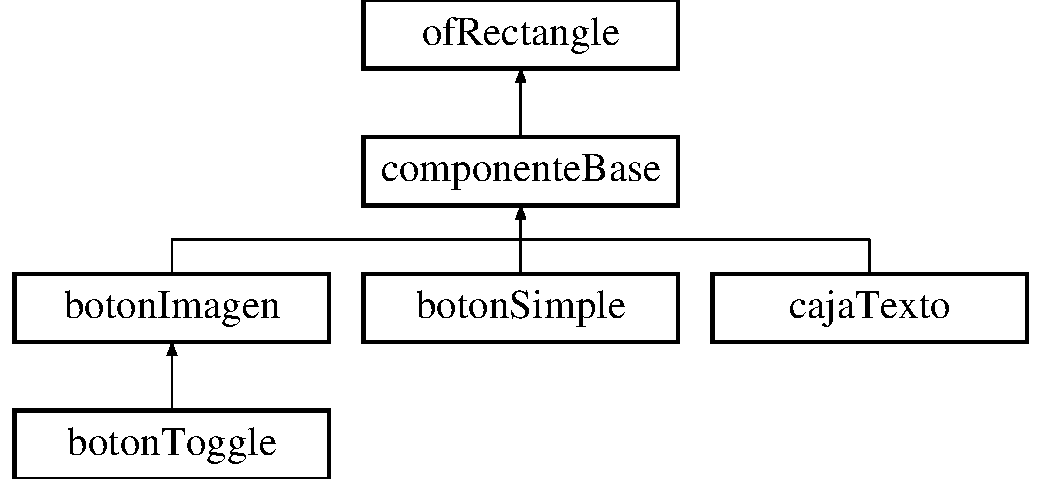
\includegraphics[height=4.000000cm]{classcomponente_base}
\end{center}
\end{figure}
\subsection*{Métodos públicos}
\begin{DoxyCompactItemize}
\item 
\hyperlink{classcomponente_base_a98286225e2be6f2080fe7d409e077a96}{componente\+Base} (int, int, int, int)
\begin{DoxyCompactList}\small\item\em Constructor de la clase. \end{DoxyCompactList}\item 
void \hyperlink{classcomponente_base_af9d40a15747b13d6cf6ac2b7b658a9d4}{set\+Tam} (int, int)
\begin{DoxyCompactList}\small\item\em Cambia el tamaño del componente. \end{DoxyCompactList}\item 
void \hyperlink{classcomponente_base_a3797a3ebadf03c8374d9c7a9460bc645}{set\+Pos} (int, int)
\begin{DoxyCompactList}\small\item\em Reposiciona el componente. \end{DoxyCompactList}\item 
bool \hyperlink{classcomponente_base_a288dc05f1eb5748ba3a24ad651623d49}{update} (float, float, float, float, bool)
\begin{DoxyCompactList}\small\item\em Actualiza el componente. \end{DoxyCompactList}\item 
virtual void \hyperlink{classcomponente_base_ac6faec0698776f8bfe0e817b9927c0f9}{draw} ()=0
\begin{DoxyCompactList}\small\item\em Dibuja el componente en pantalla. \end{DoxyCompactList}\end{DoxyCompactItemize}
\subsection*{Métodos protegidos}
\begin{DoxyCompactItemize}
\item 
bool \hyperlink{classcomponente_base_a2ca6628fb724d45687646a364ad68888}{mouse\+En\+Cuadro} (float, float)
\begin{DoxyCompactList}\small\item\em Indica si las coordenadas dadas están dentro del componente. \end{DoxyCompactList}\item 
long long int \hyperlink{classcomponente_base_a72b7c9497aa4af988a91d16446d26c34}{get\+Millisec} ()
\begin{DoxyCompactList}\small\item\em Devuelve el tiempo actual en milisegundos. \end{DoxyCompactList}\end{DoxyCompactItemize}
\subsection*{Atributos protegidos}
\begin{DoxyCompactItemize}
\item 
bool \hyperlink{classcomponente_base_ab03e8ff7fb596e34738ba00d455e37f5}{le\+Queda\+Tiempo}
\begin{DoxyCompactList}\small\item\em Indica si el usuario está fijando su atención y no ha terminado el tiempo máximo. \end{DoxyCompactList}\item 
bool \hyperlink{classcomponente_base_a3cd688b2120c9545e25b490911e66717}{mouse\+Dentro}
\begin{DoxyCompactList}\small\item\em Indice si el mouse está dentro del componente. \end{DoxyCompactList}\item 
long long int \hyperlink{classcomponente_base_a6c1aa628629954f831209628e3dfcb2b}{tiempo}
\begin{DoxyCompactList}\small\item\em Tiempo actual cuando el usuario fija su atención en el componente. \end{DoxyCompactList}\item 
int \hyperlink{classcomponente_base_a0edb9230fa502947fd80006463f9ce25}{tiempo\+Max}
\begin{DoxyCompactList}\small\item\em Tiempo máximo para activar el componente. \end{DoxyCompactList}\end{DoxyCompactItemize}


\subsection{Descripción detallada}
Esquema base de los componentes de los espacios. 

Los espacios están orientados al uso de botones con texto y/o imágenes para la interacción con el usuario. Esta clase hereda de of\+Rectangle para tener instancias de elementos rectangulares. Si se deseara un componente con otra forma geométrica es recomendable quitarle la herencia a esta clase y hacer una clase base para los componentes rectangulares. 

\subsection{Documentación del constructor y destructor}
\hypertarget{classcomponente_base_a98286225e2be6f2080fe7d409e077a96}{}\index{componente\+Base@{componente\+Base}!componente\+Base@{componente\+Base}}
\index{componente\+Base@{componente\+Base}!componente\+Base@{componente\+Base}}
\subsubsection[{componente\+Base(int, int, int, int)}]{\setlength{\rightskip}{0pt plus 5cm}componente\+Base\+::componente\+Base (
\begin{DoxyParamCaption}
\item[{int}]{\+\_\+x, }
\item[{int}]{\+\_\+y, }
\item[{int}]{\+\_\+w, }
\item[{int}]{\+\_\+h}
\end{DoxyParamCaption}
)}\label{classcomponente_base_a98286225e2be6f2080fe7d409e077a96}


Constructor de la clase. 

Todas las inicializaciones se realizan en este método. Por simpleza se omite la implementación de los métodos setup()


\begin{DoxyParams}{Parámetros}
{\em \+\_\+x} & localización en el eje x \\
\hline
{\em \+\_\+y} & localización en el eye y \\
\hline
{\em \+\_\+w} & largo del componente \\
\hline
{\em \+\_\+h} & ancho del componente \\
\hline
\end{DoxyParams}


\subsection{Documentación de las funciones miembro}
\hypertarget{classcomponente_base_ac6faec0698776f8bfe0e817b9927c0f9}{}\index{componente\+Base@{componente\+Base}!draw@{draw}}
\index{draw@{draw}!componente\+Base@{componente\+Base}}
\subsubsection[{draw()=0}]{\setlength{\rightskip}{0pt plus 5cm}virtual void componente\+Base\+::draw (
\begin{DoxyParamCaption}
{}
\end{DoxyParamCaption}
)\hspace{0.3cm}{\ttfamily [pure virtual]}}\label{classcomponente_base_ac6faec0698776f8bfe0e817b9927c0f9}


Dibuja el componente en pantalla. 



Implementado en \hyperlink{classboton_imagen_aa2f66743b229d99cc06b36f5ad16450d}{boton\+Imagen}, \hyperlink{classboton_simple_a64baaac5439d0ad0d2ec1a11e23a8ad2}{boton\+Simple} y \hyperlink{classcaja_texto_a5bc02d7f55e12fd32715e4509853a558}{caja\+Texto}.

\hypertarget{classcomponente_base_a72b7c9497aa4af988a91d16446d26c34}{}\index{componente\+Base@{componente\+Base}!get\+Millisec@{get\+Millisec}}
\index{get\+Millisec@{get\+Millisec}!componente\+Base@{componente\+Base}}
\subsubsection[{get\+Millisec()}]{\setlength{\rightskip}{0pt plus 5cm}long long int componente\+Base\+::get\+Millisec (
\begin{DoxyParamCaption}
{}
\end{DoxyParamCaption}
)\hspace{0.3cm}{\ttfamily [protected]}}\label{classcomponente_base_a72b7c9497aa4af988a91d16446d26c34}


Devuelve el tiempo actual en milisegundos. 

\hypertarget{classcomponente_base_a2ca6628fb724d45687646a364ad68888}{}\index{componente\+Base@{componente\+Base}!mouse\+En\+Cuadro@{mouse\+En\+Cuadro}}
\index{mouse\+En\+Cuadro@{mouse\+En\+Cuadro}!componente\+Base@{componente\+Base}}
\subsubsection[{mouse\+En\+Cuadro(float, float)}]{\setlength{\rightskip}{0pt plus 5cm}bool componente\+Base\+::mouse\+En\+Cuadro (
\begin{DoxyParamCaption}
\item[{float}]{x\+M, }
\item[{float}]{y\+M}
\end{DoxyParamCaption}
)\hspace{0.3cm}{\ttfamily [protected]}}\label{classcomponente_base_a2ca6628fb724d45687646a364ad68888}


Indica si las coordenadas dadas están dentro del componente. 

\hypertarget{classcomponente_base_a3797a3ebadf03c8374d9c7a9460bc645}{}\index{componente\+Base@{componente\+Base}!set\+Pos@{set\+Pos}}
\index{set\+Pos@{set\+Pos}!componente\+Base@{componente\+Base}}
\subsubsection[{set\+Pos(int, int)}]{\setlength{\rightskip}{0pt plus 5cm}void componente\+Base\+::set\+Pos (
\begin{DoxyParamCaption}
\item[{int}]{\+\_\+x, }
\item[{int}]{\+\_\+y}
\end{DoxyParamCaption}
)}\label{classcomponente_base_a3797a3ebadf03c8374d9c7a9460bc645}


Reposiciona el componente. 


\begin{DoxyParams}{Parámetros}
{\em \+\_\+x} & localización en el eje x \\
\hline
{\em \+\_\+y} & localización en el eye y \\
\hline
\end{DoxyParams}
\hypertarget{classcomponente_base_af9d40a15747b13d6cf6ac2b7b658a9d4}{}\index{componente\+Base@{componente\+Base}!set\+Tam@{set\+Tam}}
\index{set\+Tam@{set\+Tam}!componente\+Base@{componente\+Base}}
\subsubsection[{set\+Tam(int, int)}]{\setlength{\rightskip}{0pt plus 5cm}void componente\+Base\+::set\+Tam (
\begin{DoxyParamCaption}
\item[{int}]{\+\_\+w, }
\item[{int}]{\+\_\+h}
\end{DoxyParamCaption}
)}\label{classcomponente_base_af9d40a15747b13d6cf6ac2b7b658a9d4}


Cambia el tamaño del componente. 


\begin{DoxyParams}{Parámetros}
{\em \+\_\+w} & largo del componente \\
\hline
{\em \+\_\+h} & ancho del componente \\
\hline
\end{DoxyParams}
\hypertarget{classcomponente_base_a288dc05f1eb5748ba3a24ad651623d49}{}\index{componente\+Base@{componente\+Base}!update@{update}}
\index{update@{update}!componente\+Base@{componente\+Base}}
\subsubsection[{update(float, float, float, float, bool)}]{\setlength{\rightskip}{0pt plus 5cm}bool componente\+Base\+::update (
\begin{DoxyParamCaption}
\item[{float}]{x\+In, }
\item[{float}]{y\+In, }
\item[{float}]{x\+Lea, }
\item[{float}]{y\+Lea, }
\item[{bool}]{clic}
\end{DoxyParamCaption}
)}\label{classcomponente_base_a288dc05f1eb5748ba3a24ad651623d49}


Actualiza el componente. 

Valida la interacción del usuario con el componente. En caso de reconocimiento visual se usa un temporizador. Cuando el usuario fija su atención en el componente corre un temporizador, si el usuario mantiene dicha atención por ese tiempo se activa el componente. En caso de reconocimiento de gestos se utilizan la posición de entrada y un boolean que indica si el usuario hizo clic.


\begin{DoxyParams}{Parámetros}
{\em x\+In} & coordenada x de la entrada visual \\
\hline
{\em y\+In} & coordenada y de la entrada visual \\
\hline
{\em x\+Lea} & coordenada x del componente de gestos \\
\hline
{\em y\+Lea} & coordenada y del componente de gestos \\
\hline
{\em clic} & indica si el usuario ha hecho el gesto para el clic\\
\hline
\end{DoxyParams}
\begin{DoxyReturn}{Devuelve}
true si el usuario hizo clic sobre el componente 
\end{DoxyReturn}


\subsection{Documentación de los datos miembro}
\hypertarget{classcomponente_base_ab03e8ff7fb596e34738ba00d455e37f5}{}\index{componente\+Base@{componente\+Base}!le\+Queda\+Tiempo@{le\+Queda\+Tiempo}}
\index{le\+Queda\+Tiempo@{le\+Queda\+Tiempo}!componente\+Base@{componente\+Base}}
\subsubsection[{le\+Queda\+Tiempo}]{\setlength{\rightskip}{0pt plus 5cm}bool componente\+Base\+::le\+Queda\+Tiempo\hspace{0.3cm}{\ttfamily [protected]}}\label{classcomponente_base_ab03e8ff7fb596e34738ba00d455e37f5}


Indica si el usuario está fijando su atención y no ha terminado el tiempo máximo. 

\hypertarget{classcomponente_base_a3cd688b2120c9545e25b490911e66717}{}\index{componente\+Base@{componente\+Base}!mouse\+Dentro@{mouse\+Dentro}}
\index{mouse\+Dentro@{mouse\+Dentro}!componente\+Base@{componente\+Base}}
\subsubsection[{mouse\+Dentro}]{\setlength{\rightskip}{0pt plus 5cm}bool componente\+Base\+::mouse\+Dentro\hspace{0.3cm}{\ttfamily [protected]}}\label{classcomponente_base_a3cd688b2120c9545e25b490911e66717}


Indice si el mouse está dentro del componente. 

\hypertarget{classcomponente_base_a6c1aa628629954f831209628e3dfcb2b}{}\index{componente\+Base@{componente\+Base}!tiempo@{tiempo}}
\index{tiempo@{tiempo}!componente\+Base@{componente\+Base}}
\subsubsection[{tiempo}]{\setlength{\rightskip}{0pt plus 5cm}long long int componente\+Base\+::tiempo\hspace{0.3cm}{\ttfamily [protected]}}\label{classcomponente_base_a6c1aa628629954f831209628e3dfcb2b}


Tiempo actual cuando el usuario fija su atención en el componente. 

\hypertarget{classcomponente_base_a0edb9230fa502947fd80006463f9ce25}{}\index{componente\+Base@{componente\+Base}!tiempo\+Max@{tiempo\+Max}}
\index{tiempo\+Max@{tiempo\+Max}!componente\+Base@{componente\+Base}}
\subsubsection[{tiempo\+Max}]{\setlength{\rightskip}{0pt plus 5cm}int componente\+Base\+::tiempo\+Max\hspace{0.3cm}{\ttfamily [protected]}}\label{classcomponente_base_a0edb9230fa502947fd80006463f9ce25}


Tiempo máximo para activar el componente. 



La documentación para esta clase fue generada a partir de los siguientes ficheros\+:\begin{DoxyCompactItemize}
\item 
C\+:/of\+\_\+v0.\+8.\+4\+\_\+vs\+\_\+release/apps/my\+Apps/\+Robo\+Tracking\+App/src/componentes/\hyperlink{componente_base_8h}{componente\+Base.\+h}\item 
C\+:/of\+\_\+v0.\+8.\+4\+\_\+vs\+\_\+release/apps/my\+Apps/\+Robo\+Tracking\+App/src/componentes/\hyperlink{componente_base_8cpp}{componente\+Base.\+cpp}\end{DoxyCompactItemize}

\hypertarget{classconexion_yun}{}\section{Referencia de la Clase conexion\+Yun}
\label{classconexion_yun}\index{conexion\+Yun@{conexion\+Yun}}


Ayuda a enviar peticiones a un Arduino Yun.  




{\ttfamily \#include $<$conexion\+Yun.\+h$>$}

\subsection*{Métodos públicos}
\begin{DoxyCompactItemize}
\item 
\hyperlink{classconexion_yun_a80ad58e0e5786d86f6c710eda070eca8}{conexion\+Yun} (string)
\begin{DoxyCompactList}\small\item\em Constructor de la clase. \end{DoxyCompactList}\item 
string \hyperlink{classconexion_yun_aa1b77a6e64ad90c36a750a0716582d53}{enviar\+Peticion} (string)
\begin{DoxyCompactList}\small\item\em Envía una petición al Arduino. \end{DoxyCompactList}\end{DoxyCompactItemize}
\subsection*{Atributos privados}
\begin{DoxyCompactItemize}
\item 
ofx\+Xml\+Settings \hyperlink{classconexion_yun_a18a59e3f193febe142a087cc6d8d6259}{conf}
\begin{DoxyCompactList}\small\item\em Contiene las configuraciones del puerto del Arduino. \end{DoxyCompactList}\item 
string \hyperlink{classconexion_yun_a120483618dae395e425290a6fbc669f6}{direccion\+Base}
\begin{DoxyCompactList}\small\item\em Dirección en la que se encuentra el servidor del Yun. \end{DoxyCompactList}\end{DoxyCompactItemize}


\subsection{Descripción detallada}
Ayuda a enviar peticiones a un Arduino Yun. 

\subsection{Documentación del constructor y destructor}
\hypertarget{classconexion_yun_a80ad58e0e5786d86f6c710eda070eca8}{}\index{conexion\+Yun@{conexion\+Yun}!conexion\+Yun@{conexion\+Yun}}
\index{conexion\+Yun@{conexion\+Yun}!conexion\+Yun@{conexion\+Yun}}
\subsubsection[{conexion\+Yun(string)}]{\setlength{\rightskip}{0pt plus 5cm}conexion\+Yun\+::conexion\+Yun (
\begin{DoxyParamCaption}
\item[{string}]{s}
\end{DoxyParamCaption}
)}\label{classconexion_yun_a80ad58e0e5786d86f6c710eda070eca8}


Constructor de la clase. 



\subsection{Documentación de las funciones miembro}
\hypertarget{classconexion_yun_aa1b77a6e64ad90c36a750a0716582d53}{}\index{conexion\+Yun@{conexion\+Yun}!enviar\+Peticion@{enviar\+Peticion}}
\index{enviar\+Peticion@{enviar\+Peticion}!conexion\+Yun@{conexion\+Yun}}
\subsubsection[{enviar\+Peticion(string)}]{\setlength{\rightskip}{0pt plus 5cm}string conexion\+Yun\+::enviar\+Peticion (
\begin{DoxyParamCaption}
\item[{string}]{req}
\end{DoxyParamCaption}
)}\label{classconexion_yun_aa1b77a6e64ad90c36a750a0716582d53}


Envía una petición al Arduino. 



\subsection{Documentación de los datos miembro}
\hypertarget{classconexion_yun_a18a59e3f193febe142a087cc6d8d6259}{}\index{conexion\+Yun@{conexion\+Yun}!conf@{conf}}
\index{conf@{conf}!conexion\+Yun@{conexion\+Yun}}
\subsubsection[{conf}]{\setlength{\rightskip}{0pt plus 5cm}ofx\+Xml\+Settings conexion\+Yun\+::conf\hspace{0.3cm}{\ttfamily [private]}}\label{classconexion_yun_a18a59e3f193febe142a087cc6d8d6259}


Contiene las configuraciones del puerto del Arduino. 

\hypertarget{classconexion_yun_a120483618dae395e425290a6fbc669f6}{}\index{conexion\+Yun@{conexion\+Yun}!direccion\+Base@{direccion\+Base}}
\index{direccion\+Base@{direccion\+Base}!conexion\+Yun@{conexion\+Yun}}
\subsubsection[{direccion\+Base}]{\setlength{\rightskip}{0pt plus 5cm}string conexion\+Yun\+::direccion\+Base\hspace{0.3cm}{\ttfamily [private]}}\label{classconexion_yun_a120483618dae395e425290a6fbc669f6}


Dirección en la que se encuentra el servidor del Yun. 



La documentación para esta clase fue generada a partir de los siguientes ficheros\+:\begin{DoxyCompactItemize}
\item 
C\+:/of\+\_\+v0.\+8.\+4\+\_\+vs\+\_\+release/apps/my\+Apps/\+Robo\+Tracking\+App/src/utilidades/conexiones/\hyperlink{conexion_yun_8h}{conexion\+Yun.\+h}\item 
C\+:/of\+\_\+v0.\+8.\+4\+\_\+vs\+\_\+release/apps/my\+Apps/\+Robo\+Tracking\+App/src/utilidades/conexiones/\hyperlink{conexion_yun_8cpp}{conexion\+Yun.\+cpp}\end{DoxyCompactItemize}

\hypertarget{classespacio_base}{}\section{Referencia de la Clase espacio\+Base}
\label{classespacio_base}\index{espacio\+Base@{espacio\+Base}}


Clase base para todos los espacios de la aplicación.  




{\ttfamily \#include $<$espacio\+Base.\+h$>$}

Diagrama de herencias de espacio\+Base\begin{figure}[H]
\begin{center}
\leavevmode
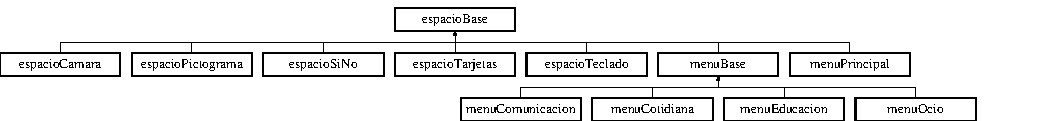
\includegraphics[height=1.615385cm]{classespacio_base}
\end{center}
\end{figure}
\subsection*{Métodos públicos}
\begin{DoxyCompactItemize}
\item 
\hyperlink{classespacio_base_a0edb5e65a20296d24f50f3fc007478d3}{espacio\+Base} (\hyperlink{classespacio_base}{espacio\+Base} $\ast$)
\begin{DoxyCompactList}\small\item\em Constructor de la clase. \end{DoxyCompactList}\item 
virtual void \hyperlink{classespacio_base_a65020ad1e767a235b0c227a1769c5416}{setup} ()=0
\begin{DoxyCompactList}\small\item\em Método inicial del ciclo de Open\+G\+L. \end{DoxyCompactList}\item 
virtual \hyperlink{classespacio_base}{espacio\+Base} $\ast$ \hyperlink{classespacio_base_a9b94b1106cd478dd78bc42078a36d013}{update} (float, float, float, float, bool)=0
\begin{DoxyCompactList}\small\item\em Controla tareas lógica de cada ciclo de Open\+G\+L. \end{DoxyCompactList}\item 
virtual void \hyperlink{classespacio_base_a01b3e668211b6159784f79a3f5a32d95}{draw} ()=0
\begin{DoxyCompactList}\small\item\em Controla las tareas gráficas de cada ciclo de Open\+G\+L. \end{DoxyCompactList}\end{DoxyCompactItemize}
\subsection*{Atributos protegidos}
\begin{DoxyCompactItemize}
\item 
\hyperlink{classespacio_base}{espacio\+Base} $\ast$ \hyperlink{classespacio_base_aa0d870b94bfc801da7bd3015fb9ce847}{espacio\+Padre}
\begin{DoxyCompactList}\small\item\em Puntero al espacio que se encarga de llamarlo. \end{DoxyCompactList}\end{DoxyCompactItemize}


\subsection{Descripción detallada}
Clase base para todos los espacios de la aplicación. 

Un espacio de la aplicación se puede ver como una pantalla. Cada pantalla está ligada a un contexto en común de la aplicación. Así pues, los espacios nuevos deben de herededar de esta clase base e implementar los debidos métodos virtuales. Si se quieren implementar los otros métodos de Open\+G\+L es recomendado que se declaren aquí pero no de manera virtual para no afectar el comportamiento de los espacios que ya existen. 

\subsection{Documentación del constructor y destructor}
\hypertarget{classespacio_base_a0edb5e65a20296d24f50f3fc007478d3}{}\index{espacio\+Base@{espacio\+Base}!espacio\+Base@{espacio\+Base}}
\index{espacio\+Base@{espacio\+Base}!espacio\+Base@{espacio\+Base}}
\subsubsection[{espacio\+Base(espacio\+Base $\ast$)}]{\setlength{\rightskip}{0pt plus 5cm}espacio\+Base\+::espacio\+Base (
\begin{DoxyParamCaption}
\item[{{\bf espacio\+Base} $\ast$}]{esp\+Padre}
\end{DoxyParamCaption}
)}\label{classespacio_base_a0edb5e65a20296d24f50f3fc007478d3}


Constructor de la clase. 

El constructor base guarda el puntero al espacio padre. Esto porque el esquema de la aplicación se ve como una jerarquía. El espacio base es el menu principal, este a su vez es padre de los submenús y estos son padres de los espacios funcionales de la aplicación. Este esquema debe ser respetado cuando se creen nuevos espacios. 

\subsection{Documentación de las funciones miembro}
\hypertarget{classespacio_base_a01b3e668211b6159784f79a3f5a32d95}{}\index{espacio\+Base@{espacio\+Base}!draw@{draw}}
\index{draw@{draw}!espacio\+Base@{espacio\+Base}}
\subsubsection[{draw()=0}]{\setlength{\rightskip}{0pt plus 5cm}virtual void espacio\+Base\+::draw (
\begin{DoxyParamCaption}
{}
\end{DoxyParamCaption}
)\hspace{0.3cm}{\ttfamily [pure virtual]}}\label{classespacio_base_a01b3e668211b6159784f79a3f5a32d95}


Controla las tareas gráficas de cada ciclo de Open\+G\+L. 



Implementado en \hyperlink{classespacio_pictograma_a0f869dd16b4431009825ef13527e40db}{espacio\+Pictograma}, \hyperlink{classmenu_base_a0faf0816595b77204dd3e0309b35b76a}{menu\+Base}, \hyperlink{classespacio_teclado_a1215fd9d4030c2642d2fbe6a4cf86589}{espacio\+Teclado}, \hyperlink{classmenu_principal_ac76c28146574b4b72364cb877b5cd83f}{menu\+Principal}, \hyperlink{classespacio_tarjetas_a53e047fce1e887a4dfc49ff31388867d}{espacio\+Tarjetas}, \hyperlink{classespacio_camara_a2c3d027a3787a226e00aab10c93f1bbe}{espacio\+Camara} y \hyperlink{classespacio_si_no_a9e413357608b8009da2f048b68220cbc}{espacio\+Si\+No}.

\hypertarget{classespacio_base_a65020ad1e767a235b0c227a1769c5416}{}\index{espacio\+Base@{espacio\+Base}!setup@{setup}}
\index{setup@{setup}!espacio\+Base@{espacio\+Base}}
\subsubsection[{setup()=0}]{\setlength{\rightskip}{0pt plus 5cm}virtual void espacio\+Base\+::setup (
\begin{DoxyParamCaption}
{}
\end{DoxyParamCaption}
)\hspace{0.3cm}{\ttfamily [pure virtual]}}\label{classespacio_base_a65020ad1e767a235b0c227a1769c5416}


Método inicial del ciclo de Open\+G\+L. 



Implementado en \hyperlink{classespacio_pictograma_a88576adb5f56ddc7d2c735f349a4864d}{espacio\+Pictograma}, \hyperlink{classmenu_base_a8d6e8078f62721431e095cb50bbcf40e}{menu\+Base}, \hyperlink{classespacio_teclado_ac6bad9b2d302639b45fbee4aed2f094d}{espacio\+Teclado}, \hyperlink{classmenu_principal_af392d4bbd2d1851b565441ed9dccbae8}{menu\+Principal}, \hyperlink{classespacio_tarjetas_a0dc8d9154c4de90daab303a4fab5fd90}{espacio\+Tarjetas}, \hyperlink{classespacio_camara_af9b840498c705d9fe3ca8e363b4a535b}{espacio\+Camara}, \hyperlink{classespacio_si_no_a4094daf8c4bcc9ca7a0303fb4c41859f}{espacio\+Si\+No}, \hyperlink{classmenu_comunicacion_a9e42e30977954e20c304261a9f1be5e1}{menu\+Comunicacion}, \hyperlink{classmenu_ocio_a6b99292a5b8c60b5a8a799447fc85f18}{menu\+Ocio} y \hyperlink{classmenu_educacion_a782815ae0152a27aca5d33885f607e81}{menu\+Educacion}.

\hypertarget{classespacio_base_a9b94b1106cd478dd78bc42078a36d013}{}\index{espacio\+Base@{espacio\+Base}!update@{update}}
\index{update@{update}!espacio\+Base@{espacio\+Base}}
\subsubsection[{update(float, float, float, float, bool)=0}]{\setlength{\rightskip}{0pt plus 5cm}virtual {\bf espacio\+Base}$\ast$ espacio\+Base\+::update (
\begin{DoxyParamCaption}
\item[{float}]{, }
\item[{float}]{, }
\item[{float}]{, }
\item[{float}]{, }
\item[{bool}]{}
\end{DoxyParamCaption}
)\hspace{0.3cm}{\ttfamily [pure virtual]}}\label{classespacio_base_a9b94b1106cd478dd78bc42078a36d013}


Controla tareas lógica de cada ciclo de Open\+G\+L. 



Implementado en \hyperlink{classespacio_pictograma_a2ebefcf2c0838ef08d067a39c307ed6d}{espacio\+Pictograma}, \hyperlink{classmenu_base_aed2125585944e1dfa0ee7cb0e4f7958c}{menu\+Base}, \hyperlink{classespacio_teclado_a0d5aa4cb23a134cfce3f00709fd2f831}{espacio\+Teclado}, \hyperlink{classmenu_principal_a69aa5c82d822246305ec9eb0ae60b546}{menu\+Principal}, \hyperlink{classespacio_tarjetas_a61d5cd1dcc3538b9eafe7a6ab7d6e6e5}{espacio\+Tarjetas}, \hyperlink{classespacio_camara_a133e544d5bb6015e3d9e6eff4a6d812d}{espacio\+Camara} y \hyperlink{classespacio_si_no_a4adfb774583e44929d17422d510b3e87}{espacio\+Si\+No}.



\subsection{Documentación de los datos miembro}
\hypertarget{classespacio_base_aa0d870b94bfc801da7bd3015fb9ce847}{}\index{espacio\+Base@{espacio\+Base}!espacio\+Padre@{espacio\+Padre}}
\index{espacio\+Padre@{espacio\+Padre}!espacio\+Base@{espacio\+Base}}
\subsubsection[{espacio\+Padre}]{\setlength{\rightskip}{0pt plus 5cm}{\bf espacio\+Base}$\ast$ espacio\+Base\+::espacio\+Padre\hspace{0.3cm}{\ttfamily [protected]}}\label{classespacio_base_aa0d870b94bfc801da7bd3015fb9ce847}


Puntero al espacio que se encarga de llamarlo. 

Este puntero es útil para cuando el usuario decide salir del espacio activo. Cualquier cambio de este comportamiento debería ser implementado de forma complementaria en esta clase. 

La documentación para esta clase fue generada a partir de los siguientes ficheros\+:\begin{DoxyCompactItemize}
\item 
C\+:/of\+\_\+v0.\+8.\+4\+\_\+vs\+\_\+release/apps/my\+Apps/\+Robo\+Tracking\+App/src/espacios/\hyperlink{espacio_base_8h}{espacio\+Base.\+h}\item 
C\+:/of\+\_\+v0.\+8.\+4\+\_\+vs\+\_\+release/apps/my\+Apps/\+Robo\+Tracking\+App/src/espacios/\hyperlink{espacio_base_8cpp}{espacio\+Base.\+cpp}\end{DoxyCompactItemize}

\hypertarget{classespacio_camara}{}\section{Referencia de la Clase espacio\+Camara}
\label{classespacio_camara}\index{espacio\+Camara@{espacio\+Camara}}


Espacio para tomar fotos por medio de la cámara.  




{\ttfamily \#include $<$espacio\+Camara.\+h$>$}

Diagrama de herencias de espacio\+Camara\begin{figure}[H]
\begin{center}
\leavevmode
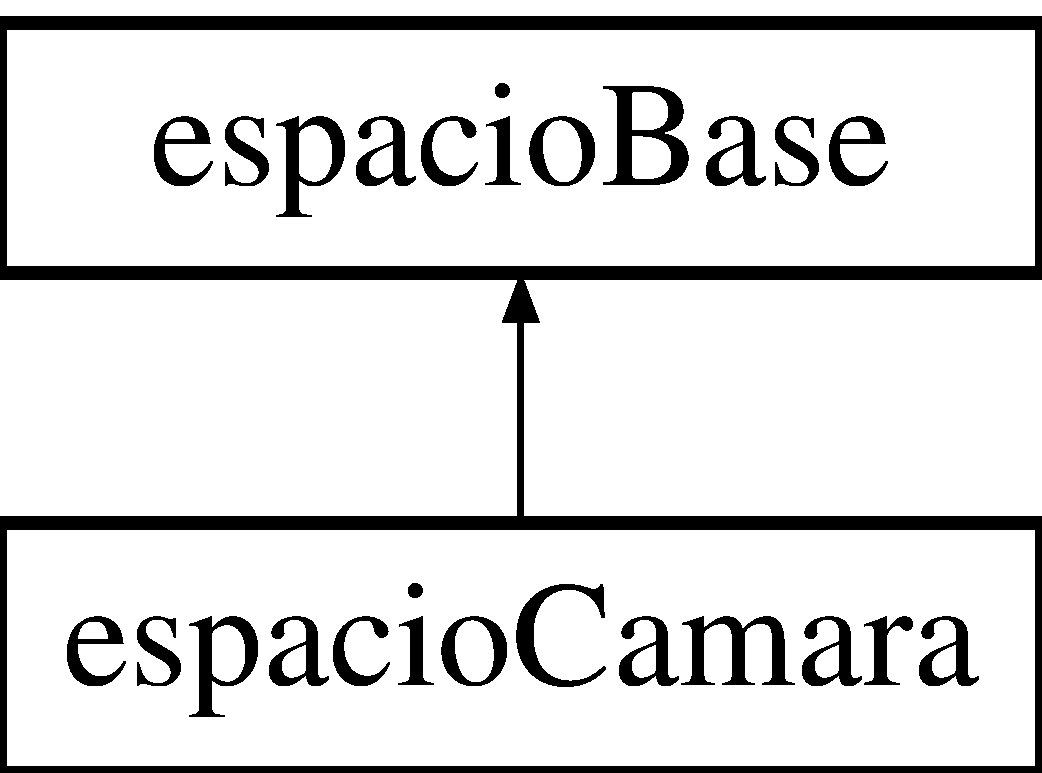
\includegraphics[height=2.000000cm]{classespacio_camara}
\end{center}
\end{figure}
\subsection*{Métodos públicos}
\begin{DoxyCompactItemize}
\item 
\hyperlink{classespacio_camara_adf85b2cd673cb9eafee260e14b9c9f41}{espacio\+Camara} (\hyperlink{classespacio_base}{espacio\+Base} $\ast$)
\begin{DoxyCompactList}\small\item\em Constructor de la clase. \end{DoxyCompactList}\item 
\hyperlink{classespacio_camara_aa6ac19fb18722f62697bfe43b1b171ce}{$\sim$espacio\+Camara} ()
\begin{DoxyCompactList}\small\item\em Destructor de la clase. \end{DoxyCompactList}\item 
void \hyperlink{classespacio_camara_af9b840498c705d9fe3ca8e363b4a535b}{setup} ()
\begin{DoxyCompactList}\small\item\em Método inicial del ciclo de Open\+G\+L. \end{DoxyCompactList}\item 
\hyperlink{classespacio_base}{espacio\+Base} $\ast$ \hyperlink{classespacio_camara_a133e544d5bb6015e3d9e6eff4a6d812d}{update} (float, float, float, float, bool)
\begin{DoxyCompactList}\small\item\em Controla tareas lógica de cada ciclo de Open\+G\+L. \end{DoxyCompactList}\item 
void \hyperlink{classespacio_camara_a2c3d027a3787a226e00aab10c93f1bbe}{draw} ()
\begin{DoxyCompactList}\small\item\em Controla las tareas gráficas de cada ciclo de Open\+G\+L. \end{DoxyCompactList}\end{DoxyCompactItemize}
\subsection*{Atributos privados}
\begin{DoxyCompactItemize}
\item 
int \hyperlink{classespacio_camara_aa357745006c6358ac4919ea079e80caa}{cam\+Width}
\begin{DoxyCompactList}\small\item\em Largo de la imagen de la cámara. \end{DoxyCompactList}\item 
int \hyperlink{classespacio_camara_ac9c3980d5710ce9ae83a95a4e7d4bf3a}{cam\+Height}
\begin{DoxyCompactList}\small\item\em Ancho de la imagen de la cámara. \end{DoxyCompactList}\item 
double \hyperlink{classespacio_camara_ac94dd88aad08d2077050c79e490d0a37}{cam\+X}
\begin{DoxyCompactList}\small\item\em Coordenada x de la imagen de la cámara. \end{DoxyCompactList}\item 
double \hyperlink{classespacio_camara_a0dec829b25bb09c1f70150f885d9843e}{cam\+Y}
\begin{DoxyCompactList}\small\item\em Coordenada y de la imagen de la cámara. \end{DoxyCompactList}\item 
of\+Video\+Grabber \hyperlink{classespacio_camara_a005166cb15e10461341d0e28b145134f}{vid\+Grabber}
\begin{DoxyCompactList}\small\item\em Instancia del manejador de la cámara. \end{DoxyCompactList}\item 
of\+Image \hyperlink{classespacio_camara_a71d14cf73376b62e3158e90a6f72d18f}{img}
\begin{DoxyCompactList}\small\item\em Captura de la cámara que se mostrando al usuario. \end{DoxyCompactList}\item 
\hyperlink{classboton_imagen}{boton\+Imagen} $\ast$ \hyperlink{classespacio_camara_a4d7caffe8a3090acf04dc78ed91e923c}{btn\+Atras}
\begin{DoxyCompactList}\small\item\em Botón para salir al menú \end{DoxyCompactList}\item 
\hyperlink{classboton_imagen}{boton\+Imagen} $\ast$ \hyperlink{classespacio_camara_a0a33e016b145a3ad2723d6d120260f48}{btn\+Foto}
\begin{DoxyCompactList}\small\item\em Botón para tomar una foto. \end{DoxyCompactList}\item 
\hyperlink{classboton_imagen}{boton\+Imagen} $\ast$ \hyperlink{classespacio_camara_a3d110b2810a8ba6579857dd7f8a6fe22}{btn\+Galeria}
\begin{DoxyCompactList}\small\item\em Botón para acceder a la galería. \end{DoxyCompactList}\end{DoxyCompactItemize}
\subsection*{Otros miembros heredados}


\subsection{Descripción detallada}
Espacio para tomar fotos por medio de la cámara. 

Este espacio define un tipo de comunicación para un usuario que posea capacidades de lectoescritura, este espacio puede mejorarse y adaptarse a las necesidades del usuario. 

\subsection{Documentación del constructor y destructor}
\hypertarget{classespacio_camara_adf85b2cd673cb9eafee260e14b9c9f41}{}\index{espacio\+Camara@{espacio\+Camara}!espacio\+Camara@{espacio\+Camara}}
\index{espacio\+Camara@{espacio\+Camara}!espacio\+Camara@{espacio\+Camara}}
\subsubsection[{espacio\+Camara(espacio\+Base $\ast$)}]{\setlength{\rightskip}{0pt plus 5cm}espacio\+Camara\+::espacio\+Camara (
\begin{DoxyParamCaption}
\item[{{\bf espacio\+Base} $\ast$}]{esp\+Padre}
\end{DoxyParamCaption}
)}\label{classespacio_camara_adf85b2cd673cb9eafee260e14b9c9f41}


Constructor de la clase. 


\begin{DoxyParams}{Parámetros}
{\em espacio\+Padre} & Puntero al menú de la categoría \\
\hline
\end{DoxyParams}
\hypertarget{classespacio_camara_aa6ac19fb18722f62697bfe43b1b171ce}{}\index{espacio\+Camara@{espacio\+Camara}!````~espacio\+Camara@{$\sim$espacio\+Camara}}
\index{````~espacio\+Camara@{$\sim$espacio\+Camara}!espacio\+Camara@{espacio\+Camara}}
\subsubsection[{$\sim$espacio\+Camara()}]{\setlength{\rightskip}{0pt plus 5cm}espacio\+Camara\+::$\sim$espacio\+Camara (
\begin{DoxyParamCaption}
{}
\end{DoxyParamCaption}
)}\label{classespacio_camara_aa6ac19fb18722f62697bfe43b1b171ce}


Destructor de la clase. 



\subsection{Documentación de las funciones miembro}
\hypertarget{classespacio_camara_a2c3d027a3787a226e00aab10c93f1bbe}{}\index{espacio\+Camara@{espacio\+Camara}!draw@{draw}}
\index{draw@{draw}!espacio\+Camara@{espacio\+Camara}}
\subsubsection[{draw()}]{\setlength{\rightskip}{0pt plus 5cm}void espacio\+Camara\+::draw (
\begin{DoxyParamCaption}
{}
\end{DoxyParamCaption}
)\hspace{0.3cm}{\ttfamily [virtual]}}\label{classespacio_camara_a2c3d027a3787a226e00aab10c93f1bbe}


Controla las tareas gráficas de cada ciclo de Open\+G\+L. 



Implementa \hyperlink{classespacio_base_a01b3e668211b6159784f79a3f5a32d95}{espacio\+Base}.

\hypertarget{classespacio_camara_af9b840498c705d9fe3ca8e363b4a535b}{}\index{espacio\+Camara@{espacio\+Camara}!setup@{setup}}
\index{setup@{setup}!espacio\+Camara@{espacio\+Camara}}
\subsubsection[{setup()}]{\setlength{\rightskip}{0pt plus 5cm}void espacio\+Camara\+::setup (
\begin{DoxyParamCaption}
{}
\end{DoxyParamCaption}
)\hspace{0.3cm}{\ttfamily [virtual]}}\label{classespacio_camara_af9b840498c705d9fe3ca8e363b4a535b}


Método inicial del ciclo de Open\+G\+L. 



Implementa \hyperlink{classespacio_base_a65020ad1e767a235b0c227a1769c5416}{espacio\+Base}.

\hypertarget{classespacio_camara_a133e544d5bb6015e3d9e6eff4a6d812d}{}\index{espacio\+Camara@{espacio\+Camara}!update@{update}}
\index{update@{update}!espacio\+Camara@{espacio\+Camara}}
\subsubsection[{update(float, float, float, float, bool)}]{\setlength{\rightskip}{0pt plus 5cm}{\bf espacio\+Base} $\ast$ espacio\+Camara\+::update (
\begin{DoxyParamCaption}
\item[{float}]{, }
\item[{float}]{, }
\item[{float}]{, }
\item[{float}]{, }
\item[{bool}]{}
\end{DoxyParamCaption}
)\hspace{0.3cm}{\ttfamily [virtual]}}\label{classespacio_camara_a133e544d5bb6015e3d9e6eff4a6d812d}


Controla tareas lógica de cada ciclo de Open\+G\+L. 



Implementa \hyperlink{classespacio_base_a9b94b1106cd478dd78bc42078a36d013}{espacio\+Base}.



\subsection{Documentación de los datos miembro}
\hypertarget{classespacio_camara_a4d7caffe8a3090acf04dc78ed91e923c}{}\index{espacio\+Camara@{espacio\+Camara}!btn\+Atras@{btn\+Atras}}
\index{btn\+Atras@{btn\+Atras}!espacio\+Camara@{espacio\+Camara}}
\subsubsection[{btn\+Atras}]{\setlength{\rightskip}{0pt plus 5cm}{\bf boton\+Imagen}$\ast$ espacio\+Camara\+::btn\+Atras\hspace{0.3cm}{\ttfamily [private]}}\label{classespacio_camara_a4d7caffe8a3090acf04dc78ed91e923c}


Botón para salir al menú 

\hypertarget{classespacio_camara_a0a33e016b145a3ad2723d6d120260f48}{}\index{espacio\+Camara@{espacio\+Camara}!btn\+Foto@{btn\+Foto}}
\index{btn\+Foto@{btn\+Foto}!espacio\+Camara@{espacio\+Camara}}
\subsubsection[{btn\+Foto}]{\setlength{\rightskip}{0pt plus 5cm}{\bf boton\+Imagen}$\ast$ espacio\+Camara\+::btn\+Foto\hspace{0.3cm}{\ttfamily [private]}}\label{classespacio_camara_a0a33e016b145a3ad2723d6d120260f48}


Botón para tomar una foto. 

\hypertarget{classespacio_camara_a3d110b2810a8ba6579857dd7f8a6fe22}{}\index{espacio\+Camara@{espacio\+Camara}!btn\+Galeria@{btn\+Galeria}}
\index{btn\+Galeria@{btn\+Galeria}!espacio\+Camara@{espacio\+Camara}}
\subsubsection[{btn\+Galeria}]{\setlength{\rightskip}{0pt plus 5cm}{\bf boton\+Imagen}$\ast$ espacio\+Camara\+::btn\+Galeria\hspace{0.3cm}{\ttfamily [private]}}\label{classespacio_camara_a3d110b2810a8ba6579857dd7f8a6fe22}


Botón para acceder a la galería. 

\hypertarget{classespacio_camara_ac9c3980d5710ce9ae83a95a4e7d4bf3a}{}\index{espacio\+Camara@{espacio\+Camara}!cam\+Height@{cam\+Height}}
\index{cam\+Height@{cam\+Height}!espacio\+Camara@{espacio\+Camara}}
\subsubsection[{cam\+Height}]{\setlength{\rightskip}{0pt plus 5cm}int espacio\+Camara\+::cam\+Height\hspace{0.3cm}{\ttfamily [private]}}\label{classespacio_camara_ac9c3980d5710ce9ae83a95a4e7d4bf3a}


Ancho de la imagen de la cámara. 

\hypertarget{classespacio_camara_aa357745006c6358ac4919ea079e80caa}{}\index{espacio\+Camara@{espacio\+Camara}!cam\+Width@{cam\+Width}}
\index{cam\+Width@{cam\+Width}!espacio\+Camara@{espacio\+Camara}}
\subsubsection[{cam\+Width}]{\setlength{\rightskip}{0pt plus 5cm}int espacio\+Camara\+::cam\+Width\hspace{0.3cm}{\ttfamily [private]}}\label{classespacio_camara_aa357745006c6358ac4919ea079e80caa}


Largo de la imagen de la cámara. 

\hypertarget{classespacio_camara_ac94dd88aad08d2077050c79e490d0a37}{}\index{espacio\+Camara@{espacio\+Camara}!cam\+X@{cam\+X}}
\index{cam\+X@{cam\+X}!espacio\+Camara@{espacio\+Camara}}
\subsubsection[{cam\+X}]{\setlength{\rightskip}{0pt plus 5cm}double espacio\+Camara\+::cam\+X\hspace{0.3cm}{\ttfamily [private]}}\label{classespacio_camara_ac94dd88aad08d2077050c79e490d0a37}


Coordenada x de la imagen de la cámara. 

\hypertarget{classespacio_camara_a0dec829b25bb09c1f70150f885d9843e}{}\index{espacio\+Camara@{espacio\+Camara}!cam\+Y@{cam\+Y}}
\index{cam\+Y@{cam\+Y}!espacio\+Camara@{espacio\+Camara}}
\subsubsection[{cam\+Y}]{\setlength{\rightskip}{0pt plus 5cm}double espacio\+Camara\+::cam\+Y\hspace{0.3cm}{\ttfamily [private]}}\label{classespacio_camara_a0dec829b25bb09c1f70150f885d9843e}


Coordenada y de la imagen de la cámara. 

\hypertarget{classespacio_camara_a71d14cf73376b62e3158e90a6f72d18f}{}\index{espacio\+Camara@{espacio\+Camara}!img@{img}}
\index{img@{img}!espacio\+Camara@{espacio\+Camara}}
\subsubsection[{img}]{\setlength{\rightskip}{0pt plus 5cm}of\+Image espacio\+Camara\+::img\hspace{0.3cm}{\ttfamily [private]}}\label{classespacio_camara_a71d14cf73376b62e3158e90a6f72d18f}


Captura de la cámara que se mostrando al usuario. 

\hypertarget{classespacio_camara_a005166cb15e10461341d0e28b145134f}{}\index{espacio\+Camara@{espacio\+Camara}!vid\+Grabber@{vid\+Grabber}}
\index{vid\+Grabber@{vid\+Grabber}!espacio\+Camara@{espacio\+Camara}}
\subsubsection[{vid\+Grabber}]{\setlength{\rightskip}{0pt plus 5cm}of\+Video\+Grabber espacio\+Camara\+::vid\+Grabber\hspace{0.3cm}{\ttfamily [private]}}\label{classespacio_camara_a005166cb15e10461341d0e28b145134f}


Instancia del manejador de la cámara. 



La documentación para esta clase fue generada a partir de los siguientes ficheros\+:\begin{DoxyCompactItemize}
\item 
C\+:/of\+\_\+v0.\+8.\+4\+\_\+vs\+\_\+release/apps/my\+Apps/\+Robo\+Tracking\+App/src/espacios/\hyperlink{espacio_camara_8h}{espacio\+Camara.\+h}\item 
C\+:/of\+\_\+v0.\+8.\+4\+\_\+vs\+\_\+release/apps/my\+Apps/\+Robo\+Tracking\+App/src/espacios/\hyperlink{espacio_camara_8cpp}{espacio\+Camara.\+cpp}\end{DoxyCompactItemize}

\hypertarget{classespacio_pictograma}{}\section{Referencia de la Clase espacio\+Pictograma}
\label{classespacio_pictograma}\index{espacio\+Pictograma@{espacio\+Pictograma}}


Espacio de comunicación por medio de pictogramas.  




{\ttfamily \#include $<$espacio\+Pictograma.\+h$>$}

Diagrama de herencias de espacio\+Pictograma\begin{figure}[H]
\begin{center}
\leavevmode
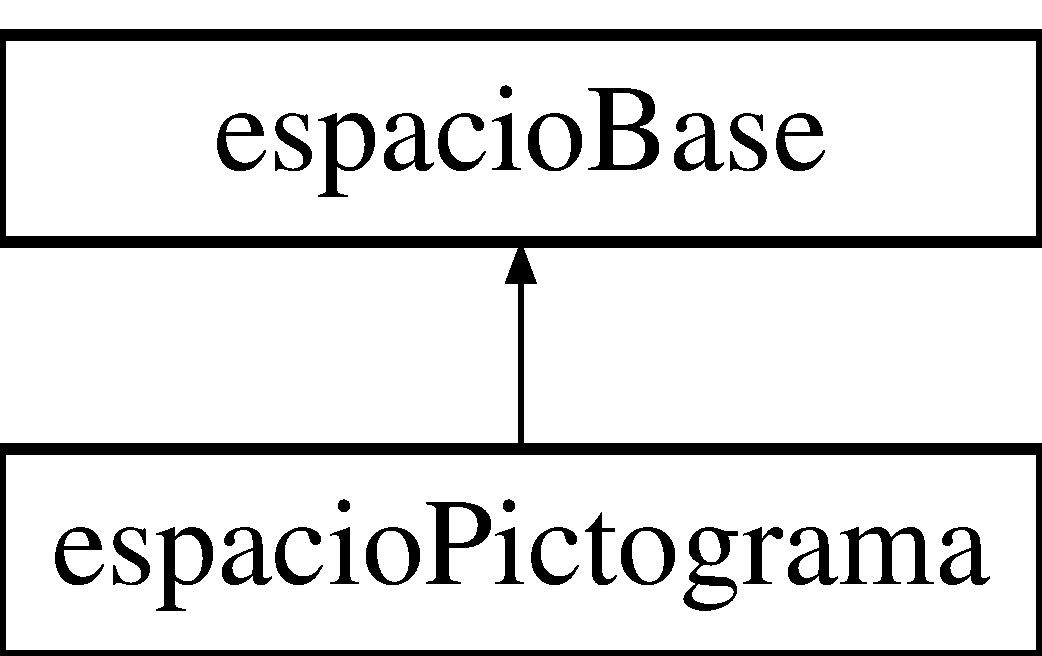
\includegraphics[height=2.000000cm]{classespacio_pictograma}
\end{center}
\end{figure}
\subsection*{Métodos públicos}
\begin{DoxyCompactItemize}
\item 
\hyperlink{classespacio_pictograma_a0f02bce6037dbf68a0fa644fd371d70c}{espacio\+Pictograma} (\hyperlink{classespacio_base}{espacio\+Base} $\ast$)
\begin{DoxyCompactList}\small\item\em Constructor de la clase. \end{DoxyCompactList}\item 
\hyperlink{classespacio_pictograma_a2dc94d6bc4ea2dec4d631d8bb8d8eb58}{$\sim$espacio\+Pictograma} ()
\begin{DoxyCompactList}\small\item\em Destructor de la clase. \end{DoxyCompactList}\item 
void \hyperlink{classespacio_pictograma_a88576adb5f56ddc7d2c735f349a4864d}{setup} ()
\begin{DoxyCompactList}\small\item\em Método inicial del ciclo de Open\+G\+L. \end{DoxyCompactList}\item 
\hyperlink{classespacio_base}{espacio\+Base} $\ast$ \hyperlink{classespacio_pictograma_aa6abbd78dd8a5e6e3eaa6976bc3b44ad}{update} (float, float)
\begin{DoxyCompactList}\small\item\em Controla tareas lógica de cada ciclo de Open\+G\+L, version tobii. \end{DoxyCompactList}\item 
\hyperlink{classespacio_base}{espacio\+Base} $\ast$ \hyperlink{classespacio_pictograma_a7483474fe025f26b200bbaecde989904}{update} (float, float, bool)
\begin{DoxyCompactList}\small\item\em Controla tareas lógica de cada ciclo de Open\+G\+L, version leap. \end{DoxyCompactList}\item 
void \hyperlink{classespacio_pictograma_a0f869dd16b4431009825ef13527e40db}{draw} ()
\begin{DoxyCompactList}\small\item\em Controla las tareas gráficas de cada ciclo de Open\+G\+L. \end{DoxyCompactList}\end{DoxyCompactItemize}
\subsection*{Métodos privados}
\begin{DoxyCompactItemize}
\item 
vector$<$ string $>$ \hyperlink{classespacio_pictograma_a298954d50054dbfe58cccb1b6b0f704d}{get\+Pictograma} (int)
\begin{DoxyCompactList}\small\item\em Recupera un pictograma de la lista cuya categoría está activa. \end{DoxyCompactList}\item 
void \hyperlink{classespacio_pictograma_abfadb8b3f6ec9c8c7558ea6eef22b295}{cargar\+Pictogramas} ()
\begin{DoxyCompactList}\small\item\em Carga los botones con los pictogramas activos. \end{DoxyCompactList}\item 
int \hyperlink{classespacio_pictograma_aa1d237a0781e86d2cc44c65c0c500d28}{get\+Tam\+Pictograma} ()
\begin{DoxyCompactList}\small\item\em Recupera la cantidad de pictogramas en una lista. \end{DoxyCompactList}\item 
void \hyperlink{classespacio_pictograma_a3a9c44580cc4f78eb1793c9479b89e9f}{comando\+Hablar} (string s)
\begin{DoxyCompactList}\small\item\em Comando temporal para texto por voz. \end{DoxyCompactList}\item 
\hyperlink{classespacio_base}{espacio\+Base} $\ast$ \hyperlink{classespacio_pictograma_a845a704901e4e675d3d871f987193fc2}{update} (bool, bool, bool, bool, bool, bool)
\end{DoxyCompactItemize}
\subsection*{Atributos privados}
\begin{DoxyCompactItemize}
\item 
\hyperlink{classboton_imagen}{boton\+Imagen} $\ast$ \hyperlink{classespacio_pictograma_ae17417de4e3122b89c29119a320888f0}{btn\+Atras}
\item 
\hyperlink{classboton_imagen}{boton\+Imagen} $\ast$ \hyperlink{classespacio_pictograma_a9157dd34f8f48cd755f721b288369dfe}{btn\+Adelante}
\item 
\hyperlink{classboton_imagen}{boton\+Imagen} $\ast$ \hyperlink{classespacio_pictograma_a739c7db68be68b07c10fe93b44a5a4d1}{btn\+Hablar}
\item 
\hyperlink{classboton_imagen}{boton\+Imagen} $\ast$ \hyperlink{classespacio_pictograma_ade5373849fab0cb55bc87bc4293e8c04}{btn\+Salir}
\item 
\hyperlink{classboton_imagen}{boton\+Imagen} $\ast$ \hyperlink{classespacio_pictograma_aa1f188f89952d7886f1d6f50f38b590f}{btn\+Borrar}
\item 
\hyperlink{classboton_imagen}{boton\+Imagen} $\ast$ \hyperlink{classespacio_pictograma_a669d076dad44b310f85b1f5dccf75568}{btn\+Borrar\+Todo}
\item 
\hyperlink{classsqlite3_manager}{sqlite3\+Manager} $\ast$ \hyperlink{classespacio_pictograma_a2e1fdcb75a25332576f897e77d1fe2de}{base\+Datos}
\begin{DoxyCompactList}\small\item\em Instancia del administrador de la base de datos. \end{DoxyCompactList}\item 
vector$<$ \hyperlink{classboton_imagen}{boton\+Imagen} $>$ \hyperlink{classespacio_pictograma_a1bee74237dc5c39e48be1f6773ca854d}{btn\+Categorias}
\begin{DoxyCompactList}\small\item\em Lista con las categorias disponibles. \end{DoxyCompactList}\item 
vector$<$ \hyperlink{classboton_imagen}{boton\+Imagen} $>$ \hyperlink{classespacio_pictograma_a7c0a60d23d55abbc5bb131fadf0210d4}{pictogramas\+Activos}
\begin{DoxyCompactList}\small\item\em Lista con los pictogramas activos. \end{DoxyCompactList}\item 
int \hyperlink{classespacio_pictograma_aa59878d6a5fe1ae995756a0a283ec5ae}{tam}
\item 
int \hyperlink{classespacio_pictograma_ae9d1d84f5ddbeba53dd9aed28e7eb0d5}{margen}
\item 
int \hyperlink{classespacio_pictograma_a3e591cd8fdedbf742f55cbc2280295bc}{offset\+X}
\item 
int \hyperlink{classespacio_pictograma_a9924df4518eadddc04074ac555e7511c}{offset\+Y}
\item 
bool \hyperlink{classespacio_pictograma_ae550974a70815794e1c2a94ccc8fd99a}{btn\+Atras\+Visible}
\begin{DoxyCompactList}\small\item\em Determina si el usuario puede devolver la lista de pictogramas. \end{DoxyCompactList}\item 
bool \hyperlink{classespacio_pictograma_aecebb0c47c0d28f31052d5084e02aec2}{btn\+Adelante\+Visible}
\begin{DoxyCompactList}\small\item\em Determina si el usuario puede continuar en la lista de pictogramas. \end{DoxyCompactList}\item 
vector$<$ vector$<$ string $>$ $>$ \hyperlink{classespacio_pictograma_a90f13e054faabc1dc26f9e62fff6f572}{str\+Categorias}
\begin{DoxyCompactList}\small\item\em Matriz con la información de las categorías. \end{DoxyCompactList}\item 
vector$<$ vector$<$ vector$<$ string $>$ $>$ $>$ \hyperlink{classespacio_pictograma_af241bdf93ef686631b46fdadf07da04a}{str\+Pictogramas}
\begin{DoxyCompactList}\small\item\em Lista de matrices con la información de los pictogramas. \end{DoxyCompactList}\item 
vector$<$ pair$<$ string, of\+Image $>$ $>$ \hyperlink{classespacio_pictograma_a46e6758b5312fa89401ff012aa2d2b92}{pictogramas\+Actuales}
\begin{DoxyCompactList}\small\item\em Lista con los pictogramas activos en la pantalla. \end{DoxyCompactList}\item 
int \hyperlink{classespacio_pictograma_ac977c8f8644a1a3ab7a724c689be0038}{indice}
\begin{DoxyCompactList}\small\item\em Indica el desplazamiento que ha hehco el usuario en la lista de pictogramas. \end{DoxyCompactList}\item 
int \hyperlink{classespacio_pictograma_ae61af3d4b032f682e7e686ca0dddbfec}{categoria\+Actual}
\begin{DoxyCompactList}\small\item\em Indica la categoría activa en la pantalla. \end{DoxyCompactList}\end{DoxyCompactItemize}
\subsection*{Otros miembros heredados}


\subsection{Descripción detallada}
Espacio de comunicación por medio de pictogramas. 

En este espacio se utliza la metodología de pictogramas como medio de comunicación. Un pictograma es un dibujo o gráfico que expresa un concepto relacionado con el objeto al que se refiere. (\href{https://es.wikipedia.org/wiki/Pictograma}{\tt https\+://es.\+wikipedia.\+org/wiki/\+Pictograma})

La información de los pictogramas están almacenados en una base de datos sqlite. La estructura del espacio consiste en categorías de pictogramas y sus respectivos gráficos. El usuario puede formar sus oraciones y luego enviarlas a texto por voz.

Los símbolos pictográficos utilizados de A\+R\+A\+S\+A\+A\+C (\href{http://catedu.es/arasaac/}{\tt http\+://catedu.\+es/arasaac/}) son parte de una obra colectiva propiedad de la Diputación General de Aragón y han creados bajo licencia Creative Commons. 

\subsection{Documentación del constructor y destructor}
\hypertarget{classespacio_pictograma_a0f02bce6037dbf68a0fa644fd371d70c}{}\index{espacio\+Pictograma@{espacio\+Pictograma}!espacio\+Pictograma@{espacio\+Pictograma}}
\index{espacio\+Pictograma@{espacio\+Pictograma}!espacio\+Pictograma@{espacio\+Pictograma}}
\subsubsection[{espacio\+Pictograma(espacio\+Base $\ast$)}]{\setlength{\rightskip}{0pt plus 5cm}espacio\+Pictograma\+::espacio\+Pictograma (
\begin{DoxyParamCaption}
\item[{{\bf espacio\+Base} $\ast$}]{esp\+Padre}
\end{DoxyParamCaption}
)}\label{classespacio_pictograma_a0f02bce6037dbf68a0fa644fd371d70c}


Constructor de la clase. 

Carga la información de los programas desde la base de datos \hypertarget{classespacio_pictograma_a2dc94d6bc4ea2dec4d631d8bb8d8eb58}{}\index{espacio\+Pictograma@{espacio\+Pictograma}!````~espacio\+Pictograma@{$\sim$espacio\+Pictograma}}
\index{````~espacio\+Pictograma@{$\sim$espacio\+Pictograma}!espacio\+Pictograma@{espacio\+Pictograma}}
\subsubsection[{$\sim$espacio\+Pictograma()}]{\setlength{\rightskip}{0pt plus 5cm}espacio\+Pictograma\+::$\sim$espacio\+Pictograma (
\begin{DoxyParamCaption}
{}
\end{DoxyParamCaption}
)}\label{classespacio_pictograma_a2dc94d6bc4ea2dec4d631d8bb8d8eb58}


Destructor de la clase. 



\subsection{Documentación de las funciones miembro}
\hypertarget{classespacio_pictograma_abfadb8b3f6ec9c8c7558ea6eef22b295}{}\index{espacio\+Pictograma@{espacio\+Pictograma}!cargar\+Pictogramas@{cargar\+Pictogramas}}
\index{cargar\+Pictogramas@{cargar\+Pictogramas}!espacio\+Pictograma@{espacio\+Pictograma}}
\subsubsection[{cargar\+Pictogramas()}]{\setlength{\rightskip}{0pt plus 5cm}void espacio\+Pictograma\+::cargar\+Pictogramas (
\begin{DoxyParamCaption}
{}
\end{DoxyParamCaption}
)\hspace{0.3cm}{\ttfamily [private]}}\label{classespacio_pictograma_abfadb8b3f6ec9c8c7558ea6eef22b295}


Carga los botones con los pictogramas activos. 

Por medio de una variable se mantiene un indice de los pictogramas activos. Por ejemplo, el indice comienza en 0 y por tanto estan activos los pictogramas 0, 1, 2 y 3 de la categoría activa. Si el índice avanza se mostrarían los pictogramas 4, 5, 6 y 7 y así hasta llegar al final de la lista. Con cada cambio de categoría el índice se reinicia. \hypertarget{classespacio_pictograma_a3a9c44580cc4f78eb1793c9479b89e9f}{}\index{espacio\+Pictograma@{espacio\+Pictograma}!comando\+Hablar@{comando\+Hablar}}
\index{comando\+Hablar@{comando\+Hablar}!espacio\+Pictograma@{espacio\+Pictograma}}
\subsubsection[{comando\+Hablar(string s)}]{\setlength{\rightskip}{0pt plus 5cm}void espacio\+Pictograma\+::comando\+Hablar (
\begin{DoxyParamCaption}
\item[{string}]{s}
\end{DoxyParamCaption}
)\hspace{0.3cm}{\ttfamily [private]}}\label{classespacio_pictograma_a3a9c44580cc4f78eb1793c9479b89e9f}


Comando temporal para texto por voz. 

\hypertarget{classespacio_pictograma_a0f869dd16b4431009825ef13527e40db}{}\index{espacio\+Pictograma@{espacio\+Pictograma}!draw@{draw}}
\index{draw@{draw}!espacio\+Pictograma@{espacio\+Pictograma}}
\subsubsection[{draw()}]{\setlength{\rightskip}{0pt plus 5cm}void espacio\+Pictograma\+::draw (
\begin{DoxyParamCaption}
{}
\end{DoxyParamCaption}
)\hspace{0.3cm}{\ttfamily [virtual]}}\label{classespacio_pictograma_a0f869dd16b4431009825ef13527e40db}


Controla las tareas gráficas de cada ciclo de Open\+G\+L. 



Implementa \hyperlink{classespacio_base_a01b3e668211b6159784f79a3f5a32d95}{espacio\+Base}.

\hypertarget{classespacio_pictograma_a298954d50054dbfe58cccb1b6b0f704d}{}\index{espacio\+Pictograma@{espacio\+Pictograma}!get\+Pictograma@{get\+Pictograma}}
\index{get\+Pictograma@{get\+Pictograma}!espacio\+Pictograma@{espacio\+Pictograma}}
\subsubsection[{get\+Pictograma(int)}]{\setlength{\rightskip}{0pt plus 5cm}vector$<$ string $>$ espacio\+Pictograma\+::get\+Pictograma (
\begin{DoxyParamCaption}
\item[{int}]{n}
\end{DoxyParamCaption}
)\hspace{0.3cm}{\ttfamily [private]}}\label{classespacio_pictograma_a298954d50054dbfe58cccb1b6b0f704d}


Recupera un pictograma de la lista cuya categoría está activa. 

\hypertarget{classespacio_pictograma_aa1d237a0781e86d2cc44c65c0c500d28}{}\index{espacio\+Pictograma@{espacio\+Pictograma}!get\+Tam\+Pictograma@{get\+Tam\+Pictograma}}
\index{get\+Tam\+Pictograma@{get\+Tam\+Pictograma}!espacio\+Pictograma@{espacio\+Pictograma}}
\subsubsection[{get\+Tam\+Pictograma()}]{\setlength{\rightskip}{0pt plus 5cm}int espacio\+Pictograma\+::get\+Tam\+Pictograma (
\begin{DoxyParamCaption}
{}
\end{DoxyParamCaption}
)\hspace{0.3cm}{\ttfamily [private]}}\label{classespacio_pictograma_aa1d237a0781e86d2cc44c65c0c500d28}


Recupera la cantidad de pictogramas en una lista. 

\hypertarget{classespacio_pictograma_a88576adb5f56ddc7d2c735f349a4864d}{}\index{espacio\+Pictograma@{espacio\+Pictograma}!setup@{setup}}
\index{setup@{setup}!espacio\+Pictograma@{espacio\+Pictograma}}
\subsubsection[{setup()}]{\setlength{\rightskip}{0pt plus 5cm}void espacio\+Pictograma\+::setup (
\begin{DoxyParamCaption}
{}
\end{DoxyParamCaption}
)\hspace{0.3cm}{\ttfamily [virtual]}}\label{classespacio_pictograma_a88576adb5f56ddc7d2c735f349a4864d}


Método inicial del ciclo de Open\+G\+L. 

Crea los botones de la categorías, los componentes del espacio y construye los botones de los pictogramas activos. 

Implementa \hyperlink{classespacio_base_a65020ad1e767a235b0c227a1769c5416}{espacio\+Base}.

\hypertarget{classespacio_pictograma_aa6abbd78dd8a5e6e3eaa6976bc3b44ad}{}\index{espacio\+Pictograma@{espacio\+Pictograma}!update@{update}}
\index{update@{update}!espacio\+Pictograma@{espacio\+Pictograma}}
\subsubsection[{update(float, float)}]{\setlength{\rightskip}{0pt plus 5cm}{\bf espacio\+Base} $\ast$ espacio\+Pictograma\+::update (
\begin{DoxyParamCaption}
\item[{float}]{, }
\item[{float}]{}
\end{DoxyParamCaption}
)\hspace{0.3cm}{\ttfamily [virtual]}}\label{classespacio_pictograma_aa6abbd78dd8a5e6e3eaa6976bc3b44ad}


Controla tareas lógica de cada ciclo de Open\+G\+L, version tobii. 



Implementa \hyperlink{classespacio_base_abb71ddaa70032182ae4d8370dd05c536}{espacio\+Base}.

\hypertarget{classespacio_pictograma_a7483474fe025f26b200bbaecde989904}{}\index{espacio\+Pictograma@{espacio\+Pictograma}!update@{update}}
\index{update@{update}!espacio\+Pictograma@{espacio\+Pictograma}}
\subsubsection[{update(float, float, bool)}]{\setlength{\rightskip}{0pt plus 5cm}{\bf espacio\+Base} $\ast$ espacio\+Pictograma\+::update (
\begin{DoxyParamCaption}
\item[{float}]{, }
\item[{float}]{, }
\item[{bool}]{}
\end{DoxyParamCaption}
)\hspace{0.3cm}{\ttfamily [virtual]}}\label{classespacio_pictograma_a7483474fe025f26b200bbaecde989904}


Controla tareas lógica de cada ciclo de Open\+G\+L, version leap. 



Implementa \hyperlink{classespacio_base_afe08700ffb54b8b8191cdea5ec1671ef}{espacio\+Base}.

\hypertarget{classespacio_pictograma_a845a704901e4e675d3d871f987193fc2}{}\index{espacio\+Pictograma@{espacio\+Pictograma}!update@{update}}
\index{update@{update}!espacio\+Pictograma@{espacio\+Pictograma}}
\subsubsection[{update(bool, bool, bool, bool, bool, bool)}]{\setlength{\rightskip}{0pt plus 5cm}{\bf espacio\+Base} $\ast$ espacio\+Pictograma\+::update (
\begin{DoxyParamCaption}
\item[{bool}]{btn\+Salir\+Res, }
\item[{bool}]{btn\+Atras\+Res, }
\item[{bool}]{btn\+Adelante\+Res, }
\item[{bool}]{btn\+Hablar\+Res, }
\item[{bool}]{btn\+Borrar\+Res, }
\item[{bool}]{btn\+Borrar\+Todo\+Res}
\end{DoxyParamCaption}
)\hspace{0.3cm}{\ttfamily [private]}}\label{classespacio_pictograma_a845a704901e4e675d3d871f987193fc2}


\subsection{Documentación de los datos miembro}
\hypertarget{classespacio_pictograma_a2e1fdcb75a25332576f897e77d1fe2de}{}\index{espacio\+Pictograma@{espacio\+Pictograma}!base\+Datos@{base\+Datos}}
\index{base\+Datos@{base\+Datos}!espacio\+Pictograma@{espacio\+Pictograma}}
\subsubsection[{base\+Datos}]{\setlength{\rightskip}{0pt plus 5cm}{\bf sqlite3\+Manager}$\ast$ espacio\+Pictograma\+::base\+Datos\hspace{0.3cm}{\ttfamily [private]}}\label{classespacio_pictograma_a2e1fdcb75a25332576f897e77d1fe2de}


Instancia del administrador de la base de datos. 

\hypertarget{classespacio_pictograma_a9157dd34f8f48cd755f721b288369dfe}{}\index{espacio\+Pictograma@{espacio\+Pictograma}!btn\+Adelante@{btn\+Adelante}}
\index{btn\+Adelante@{btn\+Adelante}!espacio\+Pictograma@{espacio\+Pictograma}}
\subsubsection[{btn\+Adelante}]{\setlength{\rightskip}{0pt plus 5cm}{\bf boton\+Imagen}$\ast$ espacio\+Pictograma\+::btn\+Adelante\hspace{0.3cm}{\ttfamily [private]}}\label{classespacio_pictograma_a9157dd34f8f48cd755f721b288369dfe}
\hypertarget{classespacio_pictograma_aecebb0c47c0d28f31052d5084e02aec2}{}\index{espacio\+Pictograma@{espacio\+Pictograma}!btn\+Adelante\+Visible@{btn\+Adelante\+Visible}}
\index{btn\+Adelante\+Visible@{btn\+Adelante\+Visible}!espacio\+Pictograma@{espacio\+Pictograma}}
\subsubsection[{btn\+Adelante\+Visible}]{\setlength{\rightskip}{0pt plus 5cm}bool espacio\+Pictograma\+::btn\+Adelante\+Visible\hspace{0.3cm}{\ttfamily [private]}}\label{classespacio_pictograma_aecebb0c47c0d28f31052d5084e02aec2}


Determina si el usuario puede continuar en la lista de pictogramas. 

\hypertarget{classespacio_pictograma_ae17417de4e3122b89c29119a320888f0}{}\index{espacio\+Pictograma@{espacio\+Pictograma}!btn\+Atras@{btn\+Atras}}
\index{btn\+Atras@{btn\+Atras}!espacio\+Pictograma@{espacio\+Pictograma}}
\subsubsection[{btn\+Atras}]{\setlength{\rightskip}{0pt plus 5cm}{\bf boton\+Imagen}$\ast$ espacio\+Pictograma\+::btn\+Atras\hspace{0.3cm}{\ttfamily [private]}}\label{classespacio_pictograma_ae17417de4e3122b89c29119a320888f0}
\hypertarget{classespacio_pictograma_ae550974a70815794e1c2a94ccc8fd99a}{}\index{espacio\+Pictograma@{espacio\+Pictograma}!btn\+Atras\+Visible@{btn\+Atras\+Visible}}
\index{btn\+Atras\+Visible@{btn\+Atras\+Visible}!espacio\+Pictograma@{espacio\+Pictograma}}
\subsubsection[{btn\+Atras\+Visible}]{\setlength{\rightskip}{0pt plus 5cm}bool espacio\+Pictograma\+::btn\+Atras\+Visible\hspace{0.3cm}{\ttfamily [private]}}\label{classespacio_pictograma_ae550974a70815794e1c2a94ccc8fd99a}


Determina si el usuario puede devolver la lista de pictogramas. 

\hypertarget{classespacio_pictograma_aa1f188f89952d7886f1d6f50f38b590f}{}\index{espacio\+Pictograma@{espacio\+Pictograma}!btn\+Borrar@{btn\+Borrar}}
\index{btn\+Borrar@{btn\+Borrar}!espacio\+Pictograma@{espacio\+Pictograma}}
\subsubsection[{btn\+Borrar}]{\setlength{\rightskip}{0pt plus 5cm}{\bf boton\+Imagen}$\ast$ espacio\+Pictograma\+::btn\+Borrar\hspace{0.3cm}{\ttfamily [private]}}\label{classespacio_pictograma_aa1f188f89952d7886f1d6f50f38b590f}
\hypertarget{classespacio_pictograma_a669d076dad44b310f85b1f5dccf75568}{}\index{espacio\+Pictograma@{espacio\+Pictograma}!btn\+Borrar\+Todo@{btn\+Borrar\+Todo}}
\index{btn\+Borrar\+Todo@{btn\+Borrar\+Todo}!espacio\+Pictograma@{espacio\+Pictograma}}
\subsubsection[{btn\+Borrar\+Todo}]{\setlength{\rightskip}{0pt plus 5cm}{\bf boton\+Imagen}$\ast$ espacio\+Pictograma\+::btn\+Borrar\+Todo\hspace{0.3cm}{\ttfamily [private]}}\label{classespacio_pictograma_a669d076dad44b310f85b1f5dccf75568}
\hypertarget{classespacio_pictograma_a1bee74237dc5c39e48be1f6773ca854d}{}\index{espacio\+Pictograma@{espacio\+Pictograma}!btn\+Categorias@{btn\+Categorias}}
\index{btn\+Categorias@{btn\+Categorias}!espacio\+Pictograma@{espacio\+Pictograma}}
\subsubsection[{btn\+Categorias}]{\setlength{\rightskip}{0pt plus 5cm}vector$<${\bf boton\+Imagen}$>$ espacio\+Pictograma\+::btn\+Categorias\hspace{0.3cm}{\ttfamily [private]}}\label{classespacio_pictograma_a1bee74237dc5c39e48be1f6773ca854d}


Lista con las categorias disponibles. 

\hypertarget{classespacio_pictograma_a739c7db68be68b07c10fe93b44a5a4d1}{}\index{espacio\+Pictograma@{espacio\+Pictograma}!btn\+Hablar@{btn\+Hablar}}
\index{btn\+Hablar@{btn\+Hablar}!espacio\+Pictograma@{espacio\+Pictograma}}
\subsubsection[{btn\+Hablar}]{\setlength{\rightskip}{0pt plus 5cm}{\bf boton\+Imagen}$\ast$ espacio\+Pictograma\+::btn\+Hablar\hspace{0.3cm}{\ttfamily [private]}}\label{classespacio_pictograma_a739c7db68be68b07c10fe93b44a5a4d1}
\hypertarget{classespacio_pictograma_ade5373849fab0cb55bc87bc4293e8c04}{}\index{espacio\+Pictograma@{espacio\+Pictograma}!btn\+Salir@{btn\+Salir}}
\index{btn\+Salir@{btn\+Salir}!espacio\+Pictograma@{espacio\+Pictograma}}
\subsubsection[{btn\+Salir}]{\setlength{\rightskip}{0pt plus 5cm}{\bf boton\+Imagen}$\ast$ espacio\+Pictograma\+::btn\+Salir\hspace{0.3cm}{\ttfamily [private]}}\label{classespacio_pictograma_ade5373849fab0cb55bc87bc4293e8c04}
\hypertarget{classespacio_pictograma_ae61af3d4b032f682e7e686ca0dddbfec}{}\index{espacio\+Pictograma@{espacio\+Pictograma}!categoria\+Actual@{categoria\+Actual}}
\index{categoria\+Actual@{categoria\+Actual}!espacio\+Pictograma@{espacio\+Pictograma}}
\subsubsection[{categoria\+Actual}]{\setlength{\rightskip}{0pt plus 5cm}int espacio\+Pictograma\+::categoria\+Actual\hspace{0.3cm}{\ttfamily [private]}}\label{classespacio_pictograma_ae61af3d4b032f682e7e686ca0dddbfec}


Indica la categoría activa en la pantalla. 

\hypertarget{classespacio_pictograma_ac977c8f8644a1a3ab7a724c689be0038}{}\index{espacio\+Pictograma@{espacio\+Pictograma}!indice@{indice}}
\index{indice@{indice}!espacio\+Pictograma@{espacio\+Pictograma}}
\subsubsection[{indice}]{\setlength{\rightskip}{0pt plus 5cm}int espacio\+Pictograma\+::indice\hspace{0.3cm}{\ttfamily [private]}}\label{classespacio_pictograma_ac977c8f8644a1a3ab7a724c689be0038}


Indica el desplazamiento que ha hehco el usuario en la lista de pictogramas. 

\hypertarget{classespacio_pictograma_ae9d1d84f5ddbeba53dd9aed28e7eb0d5}{}\index{espacio\+Pictograma@{espacio\+Pictograma}!margen@{margen}}
\index{margen@{margen}!espacio\+Pictograma@{espacio\+Pictograma}}
\subsubsection[{margen}]{\setlength{\rightskip}{0pt plus 5cm}int espacio\+Pictograma\+::margen\hspace{0.3cm}{\ttfamily [private]}}\label{classespacio_pictograma_ae9d1d84f5ddbeba53dd9aed28e7eb0d5}
\hypertarget{classespacio_pictograma_a3e591cd8fdedbf742f55cbc2280295bc}{}\index{espacio\+Pictograma@{espacio\+Pictograma}!offset\+X@{offset\+X}}
\index{offset\+X@{offset\+X}!espacio\+Pictograma@{espacio\+Pictograma}}
\subsubsection[{offset\+X}]{\setlength{\rightskip}{0pt plus 5cm}int espacio\+Pictograma\+::offset\+X\hspace{0.3cm}{\ttfamily [private]}}\label{classespacio_pictograma_a3e591cd8fdedbf742f55cbc2280295bc}
\hypertarget{classespacio_pictograma_a9924df4518eadddc04074ac555e7511c}{}\index{espacio\+Pictograma@{espacio\+Pictograma}!offset\+Y@{offset\+Y}}
\index{offset\+Y@{offset\+Y}!espacio\+Pictograma@{espacio\+Pictograma}}
\subsubsection[{offset\+Y}]{\setlength{\rightskip}{0pt plus 5cm}int espacio\+Pictograma\+::offset\+Y\hspace{0.3cm}{\ttfamily [private]}}\label{classespacio_pictograma_a9924df4518eadddc04074ac555e7511c}
\hypertarget{classespacio_pictograma_a7c0a60d23d55abbc5bb131fadf0210d4}{}\index{espacio\+Pictograma@{espacio\+Pictograma}!pictogramas\+Activos@{pictogramas\+Activos}}
\index{pictogramas\+Activos@{pictogramas\+Activos}!espacio\+Pictograma@{espacio\+Pictograma}}
\subsubsection[{pictogramas\+Activos}]{\setlength{\rightskip}{0pt plus 5cm}vector$<${\bf boton\+Imagen}$>$ espacio\+Pictograma\+::pictogramas\+Activos\hspace{0.3cm}{\ttfamily [private]}}\label{classespacio_pictograma_a7c0a60d23d55abbc5bb131fadf0210d4}


Lista con los pictogramas activos. 

\hypertarget{classespacio_pictograma_a46e6758b5312fa89401ff012aa2d2b92}{}\index{espacio\+Pictograma@{espacio\+Pictograma}!pictogramas\+Actuales@{pictogramas\+Actuales}}
\index{pictogramas\+Actuales@{pictogramas\+Actuales}!espacio\+Pictograma@{espacio\+Pictograma}}
\subsubsection[{pictogramas\+Actuales}]{\setlength{\rightskip}{0pt plus 5cm}vector$<$pair$<$string, of\+Image$>$ $>$ espacio\+Pictograma\+::pictogramas\+Actuales\hspace{0.3cm}{\ttfamily [private]}}\label{classespacio_pictograma_a46e6758b5312fa89401ff012aa2d2b92}


Lista con los pictogramas activos en la pantalla. 

\hypertarget{classespacio_pictograma_a90f13e054faabc1dc26f9e62fff6f572}{}\index{espacio\+Pictograma@{espacio\+Pictograma}!str\+Categorias@{str\+Categorias}}
\index{str\+Categorias@{str\+Categorias}!espacio\+Pictograma@{espacio\+Pictograma}}
\subsubsection[{str\+Categorias}]{\setlength{\rightskip}{0pt plus 5cm}vector$<$vector$<$string$>$ $>$ espacio\+Pictograma\+::str\+Categorias\hspace{0.3cm}{\ttfamily [private]}}\label{classespacio_pictograma_a90f13e054faabc1dc26f9e62fff6f572}


Matriz con la información de las categorías. 

\hypertarget{classespacio_pictograma_af241bdf93ef686631b46fdadf07da04a}{}\index{espacio\+Pictograma@{espacio\+Pictograma}!str\+Pictogramas@{str\+Pictogramas}}
\index{str\+Pictogramas@{str\+Pictogramas}!espacio\+Pictograma@{espacio\+Pictograma}}
\subsubsection[{str\+Pictogramas}]{\setlength{\rightskip}{0pt plus 5cm}vector$<$vector$<$vector$<$string$>$ $>$ $>$ espacio\+Pictograma\+::str\+Pictogramas\hspace{0.3cm}{\ttfamily [private]}}\label{classespacio_pictograma_af241bdf93ef686631b46fdadf07da04a}


Lista de matrices con la información de los pictogramas. 

La lista 0 corresponde a la categoría 0 y así sucesivamente para las n categorías que esten cargadas en str\+Categorias \hypertarget{classespacio_pictograma_aa59878d6a5fe1ae995756a0a283ec5ae}{}\index{espacio\+Pictograma@{espacio\+Pictograma}!tam@{tam}}
\index{tam@{tam}!espacio\+Pictograma@{espacio\+Pictograma}}
\subsubsection[{tam}]{\setlength{\rightskip}{0pt plus 5cm}int espacio\+Pictograma\+::tam\hspace{0.3cm}{\ttfamily [private]}}\label{classespacio_pictograma_aa59878d6a5fe1ae995756a0a283ec5ae}


La documentación para esta clase fue generada a partir de los siguientes ficheros\+:\begin{DoxyCompactItemize}
\item 
C\+:/of\+\_\+v0.\+8.\+4\+\_\+vs\+\_\+release/apps/my\+Apps/\+Robo\+Tracking\+App/src/espacios/\hyperlink{espacio_pictograma_8h}{espacio\+Pictograma.\+h}\item 
C\+:/of\+\_\+v0.\+8.\+4\+\_\+vs\+\_\+release/apps/my\+Apps/\+Robo\+Tracking\+App/src/espacios/\hyperlink{espacio_pictograma_8cpp}{espacio\+Pictograma.\+cpp}\end{DoxyCompactItemize}

\hypertarget{classespacio_si_no}{}\section{Referencia de la Clase espacio\+Si\+No}
\label{classespacio_si_no}\index{espacio\+Si\+No@{espacio\+Si\+No}}


Espacio de comunicación básica.  




{\ttfamily \#include $<$espacio\+Si\+No.\+h$>$}

Diagrama de herencias de espacio\+Si\+No\begin{figure}[H]
\begin{center}
\leavevmode
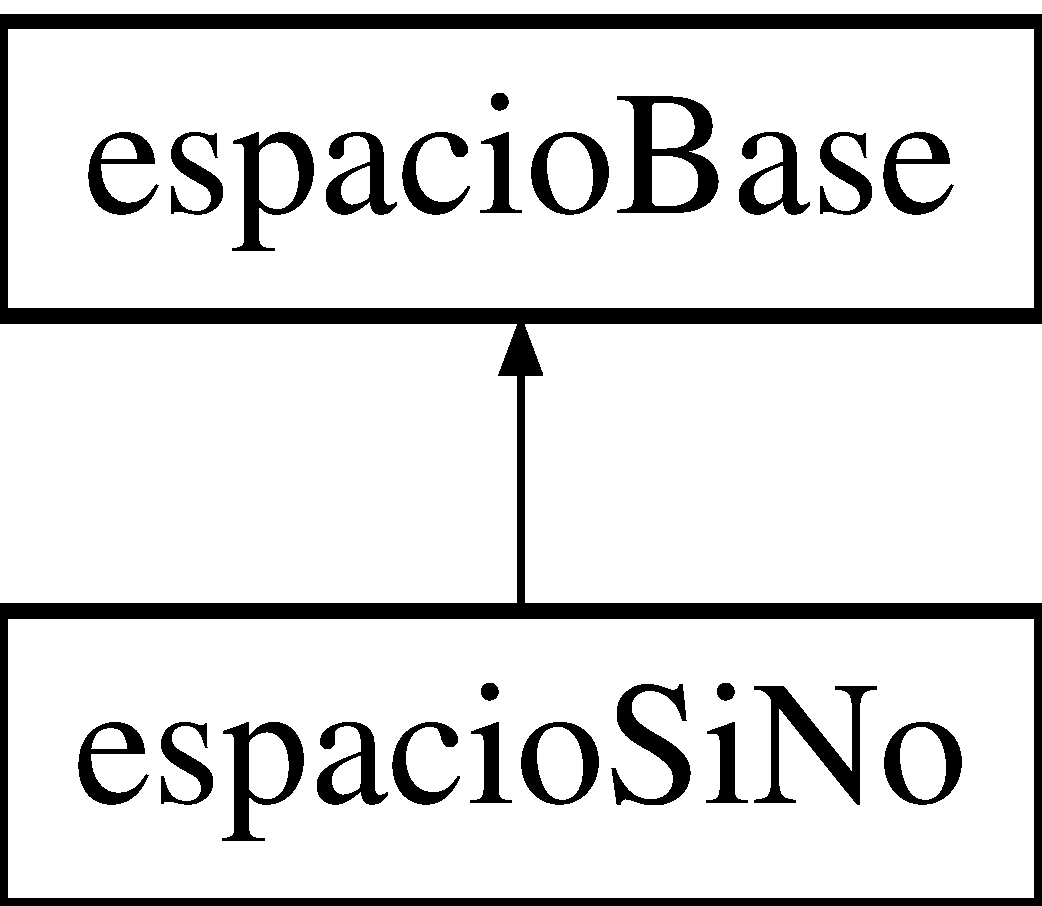
\includegraphics[height=2.000000cm]{classespacio_si_no}
\end{center}
\end{figure}
\subsection*{Métodos públicos}
\begin{DoxyCompactItemize}
\item 
\hyperlink{classespacio_si_no_ae97b5c52c884882f1adfefcc0a42d6ee}{espacio\+Si\+No} (\hyperlink{classespacio_base}{espacio\+Base} $\ast$)
\begin{DoxyCompactList}\small\item\em Constructor de la clase. \end{DoxyCompactList}\item 
\hyperlink{classespacio_si_no_a57a9a2c175f12aa908e05bb32437062e}{$\sim$espacio\+Si\+No} ()
\begin{DoxyCompactList}\small\item\em Destructor de la clase. \end{DoxyCompactList}\item 
void \hyperlink{classespacio_si_no_a4094daf8c4bcc9ca7a0303fb4c41859f}{setup} ()
\begin{DoxyCompactList}\small\item\em Método inicial del ciclo de Open\+G\+L. \end{DoxyCompactList}\item 
\hyperlink{classespacio_base}{espacio\+Base} $\ast$ \hyperlink{classespacio_si_no_a07aae24ddb49581bc81bec5acd5e898c}{update} (float, float)
\begin{DoxyCompactList}\small\item\em Controla tareas lógica de cada ciclo de Open\+G\+L, version tobii. \end{DoxyCompactList}\item 
\hyperlink{classespacio_base}{espacio\+Base} $\ast$ \hyperlink{classespacio_si_no_a555ffd236af24df46604126c1dfc8e54}{update} (float, float, bool)
\begin{DoxyCompactList}\small\item\em Controla tareas lógica de cada ciclo de Open\+G\+L, version leap. \end{DoxyCompactList}\item 
void \hyperlink{classespacio_si_no_a9e413357608b8009da2f048b68220cbc}{draw} ()
\begin{DoxyCompactList}\small\item\em Controla las tareas gráficas de cada ciclo de Open\+G\+L. \end{DoxyCompactList}\end{DoxyCompactItemize}
\subsection*{Métodos privados}
\begin{DoxyCompactItemize}
\item 
\hyperlink{classespacio_base}{espacio\+Base} $\ast$ \hyperlink{classespacio_si_no_a5f304bb286fa8e85260b0d7cb7119496}{update} (bool)
\end{DoxyCompactItemize}
\subsection*{Atributos privados}
\begin{DoxyCompactItemize}
\item 
of\+True\+Type\+Font \hyperlink{classespacio_si_no_a820d421658b6ebc4f6d09673014a60f2}{fuente\+Si\+No}
\begin{DoxyCompactList}\small\item\em Fuente para dibujar texto en pantalla. \end{DoxyCompactList}\item 
\hyperlink{classboton_imagen}{boton\+Imagen} $\ast$ \hyperlink{classespacio_si_no_ab45fe698965080072120e8ce79934a47}{btn\+Atras}
\end{DoxyCompactItemize}
\subsection*{Otros miembros heredados}


\subsection{Descripción detallada}
Espacio de comunicación básica. 

Este espacio ejemplifica un el método más simple para comunicarse. El usuario fija su atención en dos puntos, un lugar indica sí y otro indica no. 

\subsection{Documentación del constructor y destructor}
\hypertarget{classespacio_si_no_ae97b5c52c884882f1adfefcc0a42d6ee}{}\index{espacio\+Si\+No@{espacio\+Si\+No}!espacio\+Si\+No@{espacio\+Si\+No}}
\index{espacio\+Si\+No@{espacio\+Si\+No}!espacio\+Si\+No@{espacio\+Si\+No}}
\subsubsection[{espacio\+Si\+No(espacio\+Base $\ast$)}]{\setlength{\rightskip}{0pt plus 5cm}espacio\+Si\+No\+::espacio\+Si\+No (
\begin{DoxyParamCaption}
\item[{{\bf espacio\+Base} $\ast$}]{esp\+Padre}
\end{DoxyParamCaption}
)}\label{classespacio_si_no_ae97b5c52c884882f1adfefcc0a42d6ee}


Constructor de la clase. 

\hypertarget{classespacio_si_no_a57a9a2c175f12aa908e05bb32437062e}{}\index{espacio\+Si\+No@{espacio\+Si\+No}!````~espacio\+Si\+No@{$\sim$espacio\+Si\+No}}
\index{````~espacio\+Si\+No@{$\sim$espacio\+Si\+No}!espacio\+Si\+No@{espacio\+Si\+No}}
\subsubsection[{$\sim$espacio\+Si\+No()}]{\setlength{\rightskip}{0pt plus 5cm}espacio\+Si\+No\+::$\sim$espacio\+Si\+No (
\begin{DoxyParamCaption}
{}
\end{DoxyParamCaption}
)}\label{classespacio_si_no_a57a9a2c175f12aa908e05bb32437062e}


Destructor de la clase. 



\subsection{Documentación de las funciones miembro}
\hypertarget{classespacio_si_no_a9e413357608b8009da2f048b68220cbc}{}\index{espacio\+Si\+No@{espacio\+Si\+No}!draw@{draw}}
\index{draw@{draw}!espacio\+Si\+No@{espacio\+Si\+No}}
\subsubsection[{draw()}]{\setlength{\rightskip}{0pt plus 5cm}void espacio\+Si\+No\+::draw (
\begin{DoxyParamCaption}
{}
\end{DoxyParamCaption}
)\hspace{0.3cm}{\ttfamily [virtual]}}\label{classespacio_si_no_a9e413357608b8009da2f048b68220cbc}


Controla las tareas gráficas de cada ciclo de Open\+G\+L. 



Implementa \hyperlink{classespacio_base_a01b3e668211b6159784f79a3f5a32d95}{espacio\+Base}.

\hypertarget{classespacio_si_no_a4094daf8c4bcc9ca7a0303fb4c41859f}{}\index{espacio\+Si\+No@{espacio\+Si\+No}!setup@{setup}}
\index{setup@{setup}!espacio\+Si\+No@{espacio\+Si\+No}}
\subsubsection[{setup()}]{\setlength{\rightskip}{0pt plus 5cm}void espacio\+Si\+No\+::setup (
\begin{DoxyParamCaption}
{}
\end{DoxyParamCaption}
)\hspace{0.3cm}{\ttfamily [virtual]}}\label{classespacio_si_no_a4094daf8c4bcc9ca7a0303fb4c41859f}


Método inicial del ciclo de Open\+G\+L. 



Implementa \hyperlink{classespacio_base_a65020ad1e767a235b0c227a1769c5416}{espacio\+Base}.

\hypertarget{classespacio_si_no_a07aae24ddb49581bc81bec5acd5e898c}{}\index{espacio\+Si\+No@{espacio\+Si\+No}!update@{update}}
\index{update@{update}!espacio\+Si\+No@{espacio\+Si\+No}}
\subsubsection[{update(float, float)}]{\setlength{\rightskip}{0pt plus 5cm}{\bf espacio\+Base} $\ast$ espacio\+Si\+No\+::update (
\begin{DoxyParamCaption}
\item[{float}]{, }
\item[{float}]{}
\end{DoxyParamCaption}
)\hspace{0.3cm}{\ttfamily [virtual]}}\label{classespacio_si_no_a07aae24ddb49581bc81bec5acd5e898c}


Controla tareas lógica de cada ciclo de Open\+G\+L, version tobii. 



Implementa \hyperlink{classespacio_base_abb71ddaa70032182ae4d8370dd05c536}{espacio\+Base}.

\hypertarget{classespacio_si_no_a555ffd236af24df46604126c1dfc8e54}{}\index{espacio\+Si\+No@{espacio\+Si\+No}!update@{update}}
\index{update@{update}!espacio\+Si\+No@{espacio\+Si\+No}}
\subsubsection[{update(float, float, bool)}]{\setlength{\rightskip}{0pt plus 5cm}{\bf espacio\+Base} $\ast$ espacio\+Si\+No\+::update (
\begin{DoxyParamCaption}
\item[{float}]{, }
\item[{float}]{, }
\item[{bool}]{}
\end{DoxyParamCaption}
)\hspace{0.3cm}{\ttfamily [virtual]}}\label{classespacio_si_no_a555ffd236af24df46604126c1dfc8e54}


Controla tareas lógica de cada ciclo de Open\+G\+L, version leap. 



Implementa \hyperlink{classespacio_base_afe08700ffb54b8b8191cdea5ec1671ef}{espacio\+Base}.

\hypertarget{classespacio_si_no_a5f304bb286fa8e85260b0d7cb7119496}{}\index{espacio\+Si\+No@{espacio\+Si\+No}!update@{update}}
\index{update@{update}!espacio\+Si\+No@{espacio\+Si\+No}}
\subsubsection[{update(bool)}]{\setlength{\rightskip}{0pt plus 5cm}{\bf espacio\+Base} $\ast$ espacio\+Si\+No\+::update (
\begin{DoxyParamCaption}
\item[{bool}]{btn\+Atras\+Res}
\end{DoxyParamCaption}
)\hspace{0.3cm}{\ttfamily [private]}}\label{classespacio_si_no_a5f304bb286fa8e85260b0d7cb7119496}


\subsection{Documentación de los datos miembro}
\hypertarget{classespacio_si_no_ab45fe698965080072120e8ce79934a47}{}\index{espacio\+Si\+No@{espacio\+Si\+No}!btn\+Atras@{btn\+Atras}}
\index{btn\+Atras@{btn\+Atras}!espacio\+Si\+No@{espacio\+Si\+No}}
\subsubsection[{btn\+Atras}]{\setlength{\rightskip}{0pt plus 5cm}{\bf boton\+Imagen}$\ast$ espacio\+Si\+No\+::btn\+Atras\hspace{0.3cm}{\ttfamily [private]}}\label{classespacio_si_no_ab45fe698965080072120e8ce79934a47}
\hypertarget{classespacio_si_no_a820d421658b6ebc4f6d09673014a60f2}{}\index{espacio\+Si\+No@{espacio\+Si\+No}!fuente\+Si\+No@{fuente\+Si\+No}}
\index{fuente\+Si\+No@{fuente\+Si\+No}!espacio\+Si\+No@{espacio\+Si\+No}}
\subsubsection[{fuente\+Si\+No}]{\setlength{\rightskip}{0pt plus 5cm}of\+True\+Type\+Font espacio\+Si\+No\+::fuente\+Si\+No\hspace{0.3cm}{\ttfamily [private]}}\label{classespacio_si_no_a820d421658b6ebc4f6d09673014a60f2}


Fuente para dibujar texto en pantalla. 



La documentación para esta clase fue generada a partir de los siguientes ficheros\+:\begin{DoxyCompactItemize}
\item 
C\+:/of\+\_\+v0.\+8.\+4\+\_\+vs\+\_\+release/apps/my\+Apps/\+Robo\+Tracking\+App/src/espacios/\hyperlink{espacio_si_no_8h}{espacio\+Si\+No.\+h}\item 
C\+:/of\+\_\+v0.\+8.\+4\+\_\+vs\+\_\+release/apps/my\+Apps/\+Robo\+Tracking\+App/src/espacios/\hyperlink{espacio_si_no_8cpp}{espacio\+Si\+No.\+cpp}\end{DoxyCompactItemize}

\hypertarget{classespacio_tarjetas}{}\section{Referencia de la Clase espacio\+Tarjetas}
\label{classespacio_tarjetas}\index{espacio\+Tarjetas@{espacio\+Tarjetas}}


Espacio educativo donde se identifican pictogramas con su definición en palabras.  




{\ttfamily \#include $<$espacio\+Tarjetas.\+h$>$}

Diagrama de herencias de espacio\+Tarjetas\begin{figure}[H]
\begin{center}
\leavevmode
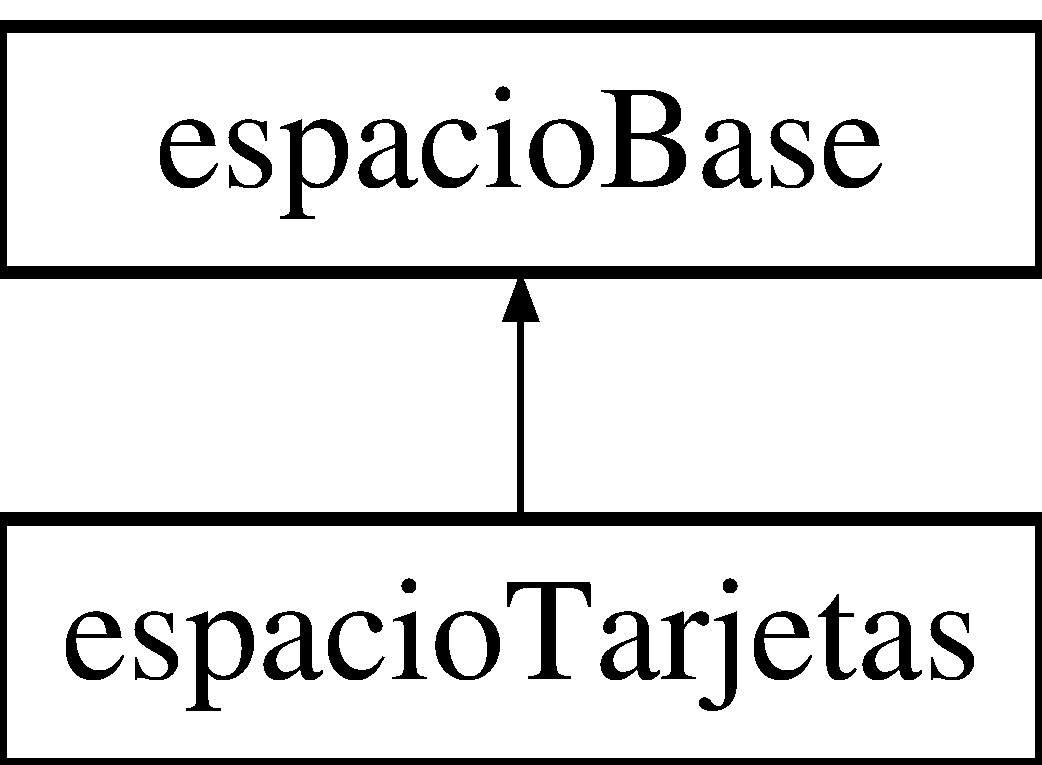
\includegraphics[height=2.000000cm]{classespacio_tarjetas}
\end{center}
\end{figure}
\subsection*{Métodos públicos}
\begin{DoxyCompactItemize}
\item 
\hyperlink{classespacio_tarjetas_a4fadd23e0a493467f5c28deecdbb975c}{espacio\+Tarjetas} (\hyperlink{classespacio_base}{espacio\+Base} $\ast$)
\begin{DoxyCompactList}\small\item\em Constructor de la clase. \end{DoxyCompactList}\item 
\hyperlink{classespacio_tarjetas_a2b5ef7680cf2193c561814d90fcc1500}{$\sim$espacio\+Tarjetas} ()
\begin{DoxyCompactList}\small\item\em Destructor de la clase. \end{DoxyCompactList}\item 
void \hyperlink{classespacio_tarjetas_a0dc8d9154c4de90daab303a4fab5fd90}{setup} ()
\begin{DoxyCompactList}\small\item\em Método inicial del ciclo de Open\+G\+L. \end{DoxyCompactList}\item 
\hyperlink{classespacio_base}{espacio\+Base} $\ast$ \hyperlink{classespacio_tarjetas_a61d5cd1dcc3538b9eafe7a6ab7d6e6e5}{update} (float, float, float, float, bool)
\begin{DoxyCompactList}\small\item\em Controla tareas lógica de cada ciclo de Open\+G\+L. \end{DoxyCompactList}\item 
void \hyperlink{classespacio_tarjetas_a53e047fce1e887a4dfc49ff31388867d}{draw} ()
\begin{DoxyCompactList}\small\item\em Controla las tareas gráficas de cada ciclo de Open\+G\+L. \end{DoxyCompactList}\end{DoxyCompactItemize}
\subsection*{Métodos privados}
\begin{DoxyCompactItemize}
\item 
void \hyperlink{classespacio_tarjetas_a14b6c40ed3154459f9b1ec511f176613}{cargar\+Tarjeta} ()
\begin{DoxyCompactList}\small\item\em Carga un ejercicio en pantalla. \end{DoxyCompactList}\item 
void \hyperlink{classespacio_tarjetas_a826269ec11513bc1c471d9aa51288a47}{validar\+Respuesta} (\hyperlink{classboton_simple}{boton\+Simple} $\ast$)
\begin{DoxyCompactList}\small\item\em Verifica si la respuesta elegida por el usuario es correcta. \end{DoxyCompactList}\end{DoxyCompactItemize}
\subsection*{Atributos privados}
\begin{DoxyCompactItemize}
\item 
vector$<$ vector$<$ string $>$ $>$ \hyperlink{classespacio_tarjetas_a4f544a79ef84de1cd86c659fad6c762c}{tarjetas}
\begin{DoxyCompactList}\small\item\em Lista con todos los pictogramas posibles. \end{DoxyCompactList}\item 
of\+Image \hyperlink{classespacio_tarjetas_afa80c75849eae23d80adb0d66ffbd540}{img}
\begin{DoxyCompactList}\small\item\em Pictograma activo que se le muestra al usuario. \end{DoxyCompactList}\item 
vector$<$ int $>$ \hyperlink{classespacio_tarjetas_a3f296834b82b6e44ebc15999d949b547}{resp}
\begin{DoxyCompactList}\small\item\em Respuestas para el pictograma activo. \end{DoxyCompactList}\item 
of\+True\+Type\+Font \hyperlink{classespacio_tarjetas_a0ae5d7269e77bc44651ca7c8f3435ef9}{fuente\+Resp}
\begin{DoxyCompactList}\small\item\em Tipo de fuente 1. \end{DoxyCompactList}\item 
of\+True\+Type\+Font \hyperlink{classespacio_tarjetas_a69c647527325428e7cb3e0c40d8f6bea}{fuente\+Resp2}
\begin{DoxyCompactList}\small\item\em Tipo de fuente 2. \end{DoxyCompactList}\item 
of\+True\+Type\+Font \hyperlink{classespacio_tarjetas_abec283907dd3683168265677e9df9659}{fuente\+Resp3}
\begin{DoxyCompactList}\small\item\em Tipo de fuente 3. \end{DoxyCompactList}\item 
\hyperlink{classboton_imagen}{boton\+Imagen} $\ast$ \hyperlink{classespacio_tarjetas_afc558908c2d0b48e3d7917722ff05a4d}{btn\+Atras}
\begin{DoxyCompactList}\small\item\em Botón para ir al menú de la categoría. \end{DoxyCompactList}\item 
\hyperlink{classboton_simple}{boton\+Simple} $\ast$ \hyperlink{classespacio_tarjetas_a1b66f906dbd856b501412a42c50da0af}{btn0}
\begin{DoxyCompactList}\small\item\em Botón para la opción 1. \end{DoxyCompactList}\item 
\hyperlink{classboton_simple}{boton\+Simple} $\ast$ \hyperlink{classespacio_tarjetas_a6f9729b868bcfef80cd3c71e22950425}{btn1}
\begin{DoxyCompactList}\small\item\em Botón para la opción 2. \end{DoxyCompactList}\item 
\hyperlink{classboton_simple}{boton\+Simple} $\ast$ \hyperlink{classespacio_tarjetas_ab0d28914026c02d7bd073d79e9c2f84e}{btn2}
\begin{DoxyCompactList}\small\item\em Botón para la opción 3. \end{DoxyCompactList}\item 
\hyperlink{classboton_simple}{boton\+Simple} $\ast$ \hyperlink{classespacio_tarjetas_a4653cac995a8e25b99d45403b626bb70}{btn3}
\begin{DoxyCompactList}\small\item\em Botón para la opción 4. \end{DoxyCompactList}\item 
\hyperlink{classboton_simple}{boton\+Simple} $\ast$ \hyperlink{classespacio_tarjetas_aa306e2b163d2a22805517fb24a728212}{btn\+Nuevo}
\begin{DoxyCompactList}\small\item\em Botón para un nuevo ejercicio. \end{DoxyCompactList}\item 
bool \hyperlink{classespacio_tarjetas_a4c37d0072ed7e82f1133641d8cdae713}{correcto}
\begin{DoxyCompactList}\small\item\em Indica si el usuario encontró la solución. \end{DoxyCompactList}\item 
bool \hyperlink{classespacio_tarjetas_aec7ea4a5a0e9f386d8d256f2444ebfaf}{incorrecto}
\begin{DoxyCompactList}\small\item\em Indica si el usuario escogió una respuesta incorrecta. \end{DoxyCompactList}\item 
\hyperlink{classsqlite3_manager}{sqlite3\+Manager} $\ast$ \hyperlink{classespacio_tarjetas_ae26629329afda23bc6252054dcad92d3}{base\+Datos}
\begin{DoxyCompactList}\small\item\em Instancia del administrador de la base de datos. \end{DoxyCompactList}\end{DoxyCompactItemize}
\subsection*{Otros miembros heredados}


\subsection{Descripción detallada}
Espacio educativo donde se identifican pictogramas con su definición en palabras. 

El usuario tiene acceso a un estilo de marque con equis, en el cual se le muesta un pictograma y 4 palabra(s). Una de la las opciones es correcta. Cuando el usuario acierta, puede volver a intentar con otro pictograma distinto.

Los símbolos pictográficos utilizados de A\+R\+A\+S\+A\+A\+C (\href{http://catedu.es/arasaac/}{\tt http\+://catedu.\+es/arasaac/}) son parte de una obra colectiva propiedad de la Diputación General de Aragón y han creados bajo licencia Creative Commons. 

\subsection{Documentación del constructor y destructor}
\hypertarget{classespacio_tarjetas_a4fadd23e0a493467f5c28deecdbb975c}{}\index{espacio\+Tarjetas@{espacio\+Tarjetas}!espacio\+Tarjetas@{espacio\+Tarjetas}}
\index{espacio\+Tarjetas@{espacio\+Tarjetas}!espacio\+Tarjetas@{espacio\+Tarjetas}}
\subsubsection[{espacio\+Tarjetas(espacio\+Base $\ast$)}]{\setlength{\rightskip}{0pt plus 5cm}espacio\+Tarjetas\+::espacio\+Tarjetas (
\begin{DoxyParamCaption}
\item[{{\bf espacio\+Base} $\ast$}]{esp\+Padre}
\end{DoxyParamCaption}
)}\label{classespacio_tarjetas_a4fadd23e0a493467f5c28deecdbb975c}


Constructor de la clase. 

\hypertarget{classespacio_tarjetas_a2b5ef7680cf2193c561814d90fcc1500}{}\index{espacio\+Tarjetas@{espacio\+Tarjetas}!````~espacio\+Tarjetas@{$\sim$espacio\+Tarjetas}}
\index{````~espacio\+Tarjetas@{$\sim$espacio\+Tarjetas}!espacio\+Tarjetas@{espacio\+Tarjetas}}
\subsubsection[{$\sim$espacio\+Tarjetas()}]{\setlength{\rightskip}{0pt plus 5cm}espacio\+Tarjetas\+::$\sim$espacio\+Tarjetas (
\begin{DoxyParamCaption}
{}
\end{DoxyParamCaption}
)}\label{classespacio_tarjetas_a2b5ef7680cf2193c561814d90fcc1500}


Destructor de la clase. 



\subsection{Documentación de las funciones miembro}
\hypertarget{classespacio_tarjetas_a14b6c40ed3154459f9b1ec511f176613}{}\index{espacio\+Tarjetas@{espacio\+Tarjetas}!cargar\+Tarjeta@{cargar\+Tarjeta}}
\index{cargar\+Tarjeta@{cargar\+Tarjeta}!espacio\+Tarjetas@{espacio\+Tarjetas}}
\subsubsection[{cargar\+Tarjeta()}]{\setlength{\rightskip}{0pt plus 5cm}void espacio\+Tarjetas\+::cargar\+Tarjeta (
\begin{DoxyParamCaption}
{}
\end{DoxyParamCaption}
)\hspace{0.3cm}{\ttfamily [private]}}\label{classespacio_tarjetas_a14b6c40ed3154459f9b1ec511f176613}


Carga un ejercicio en pantalla. 

\hypertarget{classespacio_tarjetas_a53e047fce1e887a4dfc49ff31388867d}{}\index{espacio\+Tarjetas@{espacio\+Tarjetas}!draw@{draw}}
\index{draw@{draw}!espacio\+Tarjetas@{espacio\+Tarjetas}}
\subsubsection[{draw()}]{\setlength{\rightskip}{0pt plus 5cm}void espacio\+Tarjetas\+::draw (
\begin{DoxyParamCaption}
{}
\end{DoxyParamCaption}
)\hspace{0.3cm}{\ttfamily [virtual]}}\label{classespacio_tarjetas_a53e047fce1e887a4dfc49ff31388867d}


Controla las tareas gráficas de cada ciclo de Open\+G\+L. 



Implementa \hyperlink{classespacio_base_a01b3e668211b6159784f79a3f5a32d95}{espacio\+Base}.

\hypertarget{classespacio_tarjetas_a0dc8d9154c4de90daab303a4fab5fd90}{}\index{espacio\+Tarjetas@{espacio\+Tarjetas}!setup@{setup}}
\index{setup@{setup}!espacio\+Tarjetas@{espacio\+Tarjetas}}
\subsubsection[{setup()}]{\setlength{\rightskip}{0pt plus 5cm}void espacio\+Tarjetas\+::setup (
\begin{DoxyParamCaption}
{}
\end{DoxyParamCaption}
)\hspace{0.3cm}{\ttfamily [virtual]}}\label{classespacio_tarjetas_a0dc8d9154c4de90daab303a4fab5fd90}


Método inicial del ciclo de Open\+G\+L. 



Implementa \hyperlink{classespacio_base_a65020ad1e767a235b0c227a1769c5416}{espacio\+Base}.

\hypertarget{classespacio_tarjetas_a61d5cd1dcc3538b9eafe7a6ab7d6e6e5}{}\index{espacio\+Tarjetas@{espacio\+Tarjetas}!update@{update}}
\index{update@{update}!espacio\+Tarjetas@{espacio\+Tarjetas}}
\subsubsection[{update(float, float, float, float, bool)}]{\setlength{\rightskip}{0pt plus 5cm}{\bf espacio\+Base} $\ast$ espacio\+Tarjetas\+::update (
\begin{DoxyParamCaption}
\item[{float}]{, }
\item[{float}]{, }
\item[{float}]{, }
\item[{float}]{, }
\item[{bool}]{}
\end{DoxyParamCaption}
)\hspace{0.3cm}{\ttfamily [virtual]}}\label{classespacio_tarjetas_a61d5cd1dcc3538b9eafe7a6ab7d6e6e5}


Controla tareas lógica de cada ciclo de Open\+G\+L. 



Implementa \hyperlink{classespacio_base_a9b94b1106cd478dd78bc42078a36d013}{espacio\+Base}.

\hypertarget{classespacio_tarjetas_a826269ec11513bc1c471d9aa51288a47}{}\index{espacio\+Tarjetas@{espacio\+Tarjetas}!validar\+Respuesta@{validar\+Respuesta}}
\index{validar\+Respuesta@{validar\+Respuesta}!espacio\+Tarjetas@{espacio\+Tarjetas}}
\subsubsection[{validar\+Respuesta(boton\+Simple $\ast$)}]{\setlength{\rightskip}{0pt plus 5cm}void espacio\+Tarjetas\+::validar\+Respuesta (
\begin{DoxyParamCaption}
\item[{{\bf boton\+Simple} $\ast$}]{btn}
\end{DoxyParamCaption}
)\hspace{0.3cm}{\ttfamily [private]}}\label{classespacio_tarjetas_a826269ec11513bc1c471d9aa51288a47}


Verifica si la respuesta elegida por el usuario es correcta. 



\subsection{Documentación de los datos miembro}
\hypertarget{classespacio_tarjetas_ae26629329afda23bc6252054dcad92d3}{}\index{espacio\+Tarjetas@{espacio\+Tarjetas}!base\+Datos@{base\+Datos}}
\index{base\+Datos@{base\+Datos}!espacio\+Tarjetas@{espacio\+Tarjetas}}
\subsubsection[{base\+Datos}]{\setlength{\rightskip}{0pt plus 5cm}{\bf sqlite3\+Manager}$\ast$ espacio\+Tarjetas\+::base\+Datos\hspace{0.3cm}{\ttfamily [private]}}\label{classespacio_tarjetas_ae26629329afda23bc6252054dcad92d3}


Instancia del administrador de la base de datos. 

\hypertarget{classespacio_tarjetas_a1b66f906dbd856b501412a42c50da0af}{}\index{espacio\+Tarjetas@{espacio\+Tarjetas}!btn0@{btn0}}
\index{btn0@{btn0}!espacio\+Tarjetas@{espacio\+Tarjetas}}
\subsubsection[{btn0}]{\setlength{\rightskip}{0pt plus 5cm}{\bf boton\+Simple}$\ast$ espacio\+Tarjetas\+::btn0\hspace{0.3cm}{\ttfamily [private]}}\label{classespacio_tarjetas_a1b66f906dbd856b501412a42c50da0af}


Botón para la opción 1. 

\hypertarget{classespacio_tarjetas_a6f9729b868bcfef80cd3c71e22950425}{}\index{espacio\+Tarjetas@{espacio\+Tarjetas}!btn1@{btn1}}
\index{btn1@{btn1}!espacio\+Tarjetas@{espacio\+Tarjetas}}
\subsubsection[{btn1}]{\setlength{\rightskip}{0pt plus 5cm}{\bf boton\+Simple}$\ast$ espacio\+Tarjetas\+::btn1\hspace{0.3cm}{\ttfamily [private]}}\label{classespacio_tarjetas_a6f9729b868bcfef80cd3c71e22950425}


Botón para la opción 2. 

\hypertarget{classespacio_tarjetas_ab0d28914026c02d7bd073d79e9c2f84e}{}\index{espacio\+Tarjetas@{espacio\+Tarjetas}!btn2@{btn2}}
\index{btn2@{btn2}!espacio\+Tarjetas@{espacio\+Tarjetas}}
\subsubsection[{btn2}]{\setlength{\rightskip}{0pt plus 5cm}{\bf boton\+Simple}$\ast$ espacio\+Tarjetas\+::btn2\hspace{0.3cm}{\ttfamily [private]}}\label{classespacio_tarjetas_ab0d28914026c02d7bd073d79e9c2f84e}


Botón para la opción 3. 

\hypertarget{classespacio_tarjetas_a4653cac995a8e25b99d45403b626bb70}{}\index{espacio\+Tarjetas@{espacio\+Tarjetas}!btn3@{btn3}}
\index{btn3@{btn3}!espacio\+Tarjetas@{espacio\+Tarjetas}}
\subsubsection[{btn3}]{\setlength{\rightskip}{0pt plus 5cm}{\bf boton\+Simple}$\ast$ espacio\+Tarjetas\+::btn3\hspace{0.3cm}{\ttfamily [private]}}\label{classespacio_tarjetas_a4653cac995a8e25b99d45403b626bb70}


Botón para la opción 4. 

\hypertarget{classespacio_tarjetas_afc558908c2d0b48e3d7917722ff05a4d}{}\index{espacio\+Tarjetas@{espacio\+Tarjetas}!btn\+Atras@{btn\+Atras}}
\index{btn\+Atras@{btn\+Atras}!espacio\+Tarjetas@{espacio\+Tarjetas}}
\subsubsection[{btn\+Atras}]{\setlength{\rightskip}{0pt plus 5cm}{\bf boton\+Imagen}$\ast$ espacio\+Tarjetas\+::btn\+Atras\hspace{0.3cm}{\ttfamily [private]}}\label{classespacio_tarjetas_afc558908c2d0b48e3d7917722ff05a4d}


Botón para ir al menú de la categoría. 

\hypertarget{classespacio_tarjetas_aa306e2b163d2a22805517fb24a728212}{}\index{espacio\+Tarjetas@{espacio\+Tarjetas}!btn\+Nuevo@{btn\+Nuevo}}
\index{btn\+Nuevo@{btn\+Nuevo}!espacio\+Tarjetas@{espacio\+Tarjetas}}
\subsubsection[{btn\+Nuevo}]{\setlength{\rightskip}{0pt plus 5cm}{\bf boton\+Simple}$\ast$ espacio\+Tarjetas\+::btn\+Nuevo\hspace{0.3cm}{\ttfamily [private]}}\label{classespacio_tarjetas_aa306e2b163d2a22805517fb24a728212}


Botón para un nuevo ejercicio. 

\hypertarget{classespacio_tarjetas_a4c37d0072ed7e82f1133641d8cdae713}{}\index{espacio\+Tarjetas@{espacio\+Tarjetas}!correcto@{correcto}}
\index{correcto@{correcto}!espacio\+Tarjetas@{espacio\+Tarjetas}}
\subsubsection[{correcto}]{\setlength{\rightskip}{0pt plus 5cm}bool espacio\+Tarjetas\+::correcto\hspace{0.3cm}{\ttfamily [private]}}\label{classespacio_tarjetas_a4c37d0072ed7e82f1133641d8cdae713}


Indica si el usuario encontró la solución. 

\hypertarget{classespacio_tarjetas_a0ae5d7269e77bc44651ca7c8f3435ef9}{}\index{espacio\+Tarjetas@{espacio\+Tarjetas}!fuente\+Resp@{fuente\+Resp}}
\index{fuente\+Resp@{fuente\+Resp}!espacio\+Tarjetas@{espacio\+Tarjetas}}
\subsubsection[{fuente\+Resp}]{\setlength{\rightskip}{0pt plus 5cm}of\+True\+Type\+Font espacio\+Tarjetas\+::fuente\+Resp\hspace{0.3cm}{\ttfamily [private]}}\label{classespacio_tarjetas_a0ae5d7269e77bc44651ca7c8f3435ef9}


Tipo de fuente 1. 

\hypertarget{classespacio_tarjetas_a69c647527325428e7cb3e0c40d8f6bea}{}\index{espacio\+Tarjetas@{espacio\+Tarjetas}!fuente\+Resp2@{fuente\+Resp2}}
\index{fuente\+Resp2@{fuente\+Resp2}!espacio\+Tarjetas@{espacio\+Tarjetas}}
\subsubsection[{fuente\+Resp2}]{\setlength{\rightskip}{0pt plus 5cm}of\+True\+Type\+Font espacio\+Tarjetas\+::fuente\+Resp2\hspace{0.3cm}{\ttfamily [private]}}\label{classespacio_tarjetas_a69c647527325428e7cb3e0c40d8f6bea}


Tipo de fuente 2. 

\hypertarget{classespacio_tarjetas_abec283907dd3683168265677e9df9659}{}\index{espacio\+Tarjetas@{espacio\+Tarjetas}!fuente\+Resp3@{fuente\+Resp3}}
\index{fuente\+Resp3@{fuente\+Resp3}!espacio\+Tarjetas@{espacio\+Tarjetas}}
\subsubsection[{fuente\+Resp3}]{\setlength{\rightskip}{0pt plus 5cm}of\+True\+Type\+Font espacio\+Tarjetas\+::fuente\+Resp3\hspace{0.3cm}{\ttfamily [private]}}\label{classespacio_tarjetas_abec283907dd3683168265677e9df9659}


Tipo de fuente 3. 

\hypertarget{classespacio_tarjetas_afa80c75849eae23d80adb0d66ffbd540}{}\index{espacio\+Tarjetas@{espacio\+Tarjetas}!img@{img}}
\index{img@{img}!espacio\+Tarjetas@{espacio\+Tarjetas}}
\subsubsection[{img}]{\setlength{\rightskip}{0pt plus 5cm}of\+Image espacio\+Tarjetas\+::img\hspace{0.3cm}{\ttfamily [private]}}\label{classespacio_tarjetas_afa80c75849eae23d80adb0d66ffbd540}


Pictograma activo que se le muestra al usuario. 

\hypertarget{classespacio_tarjetas_aec7ea4a5a0e9f386d8d256f2444ebfaf}{}\index{espacio\+Tarjetas@{espacio\+Tarjetas}!incorrecto@{incorrecto}}
\index{incorrecto@{incorrecto}!espacio\+Tarjetas@{espacio\+Tarjetas}}
\subsubsection[{incorrecto}]{\setlength{\rightskip}{0pt plus 5cm}bool espacio\+Tarjetas\+::incorrecto\hspace{0.3cm}{\ttfamily [private]}}\label{classespacio_tarjetas_aec7ea4a5a0e9f386d8d256f2444ebfaf}


Indica si el usuario escogió una respuesta incorrecta. 

\hypertarget{classespacio_tarjetas_a3f296834b82b6e44ebc15999d949b547}{}\index{espacio\+Tarjetas@{espacio\+Tarjetas}!resp@{resp}}
\index{resp@{resp}!espacio\+Tarjetas@{espacio\+Tarjetas}}
\subsubsection[{resp}]{\setlength{\rightskip}{0pt plus 5cm}vector$<$int$>$ espacio\+Tarjetas\+::resp\hspace{0.3cm}{\ttfamily [private]}}\label{classespacio_tarjetas_a3f296834b82b6e44ebc15999d949b547}


Respuestas para el pictograma activo. 

\hypertarget{classespacio_tarjetas_a4f544a79ef84de1cd86c659fad6c762c}{}\index{espacio\+Tarjetas@{espacio\+Tarjetas}!tarjetas@{tarjetas}}
\index{tarjetas@{tarjetas}!espacio\+Tarjetas@{espacio\+Tarjetas}}
\subsubsection[{tarjetas}]{\setlength{\rightskip}{0pt plus 5cm}vector$<$vector$<$string$>$ $>$ espacio\+Tarjetas\+::tarjetas\hspace{0.3cm}{\ttfamily [private]}}\label{classespacio_tarjetas_a4f544a79ef84de1cd86c659fad6c762c}


Lista con todos los pictogramas posibles. 

Esta lista se carga por medio de la base de datos sqlite 

La documentación para esta clase fue generada a partir de los siguientes ficheros\+:\begin{DoxyCompactItemize}
\item 
C\+:/of\+\_\+v0.\+8.\+4\+\_\+vs\+\_\+release/apps/my\+Apps/\+Robo\+Tracking\+App/src/espacios/\hyperlink{espacio_tarjetas_8h}{espacio\+Tarjetas.\+h}\item 
C\+:/of\+\_\+v0.\+8.\+4\+\_\+vs\+\_\+release/apps/my\+Apps/\+Robo\+Tracking\+App/src/espacios/\hyperlink{espacio_tarjetas_8cpp}{espacio\+Tarjetas.\+cpp}\end{DoxyCompactItemize}

\hypertarget{classespacio_teclado}{}\section{Referencia de la Clase espacio\+Teclado}
\label{classespacio_teclado}\index{espacio\+Teclado@{espacio\+Teclado}}


Espacio de comunicación por medio de lecto escritura.  




{\ttfamily \#include $<$espacio\+Teclado.\+h$>$}

Diagrama de herencias de espacio\+Teclado\begin{figure}[H]
\begin{center}
\leavevmode
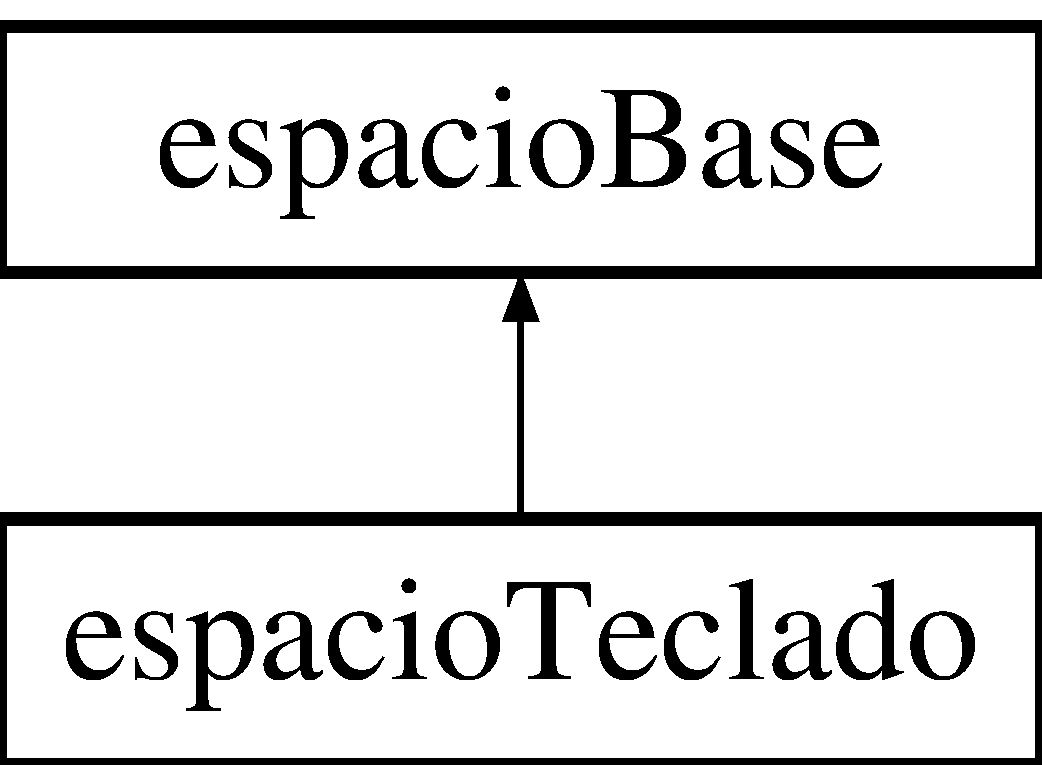
\includegraphics[height=2.000000cm]{classespacio_teclado}
\end{center}
\end{figure}
\subsection*{Métodos públicos}
\begin{DoxyCompactItemize}
\item 
\hyperlink{classespacio_teclado_a7bdaaa950b5673a464f322382aaf95cd}{espacio\+Teclado} (string, \hyperlink{classespacio_base}{espacio\+Base} $\ast$)
\begin{DoxyCompactList}\small\item\em Constructor de la clase. \end{DoxyCompactList}\item 
\hyperlink{classespacio_teclado_a98b147b70f0ce7a5bc6805d786f84cc4}{$\sim$espacio\+Teclado} ()
\begin{DoxyCompactList}\small\item\em Destructor de la clase. \end{DoxyCompactList}\item 
void \hyperlink{classespacio_teclado_ac6bad9b2d302639b45fbee4aed2f094d}{setup} ()
\begin{DoxyCompactList}\small\item\em Método inicial del ciclo de Open\+G\+L. \end{DoxyCompactList}\item 
\hyperlink{classespacio_base}{espacio\+Base} $\ast$ \hyperlink{classespacio_teclado_a0d5aa4cb23a134cfce3f00709fd2f831}{update} (float, float, float, float, bool)
\begin{DoxyCompactList}\small\item\em Controla tareas lógica de cada ciclo de Open\+G\+L. \end{DoxyCompactList}\item 
void \hyperlink{classespacio_teclado_a1215fd9d4030c2642d2fbe6a4cf86589}{draw} ()
\begin{DoxyCompactList}\small\item\em Controla las tareas gráficas de cada ciclo de Open\+G\+L. \end{DoxyCompactList}\end{DoxyCompactItemize}
\subsection*{Métodos privados}
\begin{DoxyCompactItemize}
\item 
void \hyperlink{classespacio_teclado_a02159fdf23f2e54c39be99dce372011f}{comando\+Hablar} (string)
\begin{DoxyCompactList}\small\item\em Envía el texto al sintetizador de voz. \end{DoxyCompactList}\end{DoxyCompactItemize}
\subsection*{Atributos privados}
\begin{DoxyCompactItemize}
\item 
ofx\+Xml\+Settings \hyperlink{classespacio_teclado_af215829331b2ed6d0a4485eab2a37311}{configuraciones}
\begin{DoxyCompactList}\small\item\em Instancia del manejador del archivo de configuraciones. \end{DoxyCompactList}\item 
\hyperlink{classfabrica_componentes}{fabrica\+Componentes} \hyperlink{classespacio_teclado_aaa53bfd0abe00de252f38c299174f0d1}{fab\+Componentes}
\begin{DoxyCompactList}\small\item\em Fabrica los componentes a partir de las configuraciones. \end{DoxyCompactList}\item 
int \hyperlink{classespacio_teclado_ac6f638174ab5143b45b5a0658f6782e9}{cantidad\+Componentes}
\begin{DoxyCompactList}\small\item\em Cantidad de componentes en la pantalla. \end{DoxyCompactList}\item 
vector$<$ \hyperlink{classcomponente_base}{componente\+Base} $\ast$ $>$ \hyperlink{classespacio_teclado_aad1549ce795db466bad7c47a5f82582c}{componentes}
\begin{DoxyCompactList}\small\item\em Lista con los componentes cargados de las configuraciones. \end{DoxyCompactList}\item 
\hyperlink{classcaja_texto}{caja\+Texto} $\ast$ \hyperlink{classespacio_teclado_ac4d882599a627a2d26aa19280fb1cf28}{c\+Texto}
\begin{DoxyCompactList}\small\item\em Caja de texto para mostrar la hilera que produce el usuario. \end{DoxyCompactList}\item 
\hyperlink{classboton_simple}{boton\+Simple} $\ast$ \hyperlink{classespacio_teclado_a68242d035fdf24a605e21d798ecf1a93}{btn\+Borrar}
\begin{DoxyCompactList}\small\item\em Botón para borrar el último caracter. \end{DoxyCompactList}\item 
\hyperlink{classboton_simple}{boton\+Simple} $\ast$ \hyperlink{classespacio_teclado_abf7bb12c95256d20e421831fea3d23e1}{btn\+Espacio}
\begin{DoxyCompactList}\small\item\em Botón para insertar un nuevo espacio. \end{DoxyCompactList}\item 
\hyperlink{classboton_simple}{boton\+Simple} $\ast$ \hyperlink{classespacio_teclado_a401d7d71c05c9f234010e33adfe51d04}{btn\+Hablar}
\begin{DoxyCompactList}\small\item\em Botón para pasar la hilera a voz. \end{DoxyCompactList}\item 
\hyperlink{classboton_imagen}{boton\+Imagen} $\ast$ \hyperlink{classespacio_teclado_a82d9f915e17ee3491992da61a0d28a8f}{btn\+Salir}
\begin{DoxyCompactList}\small\item\em Botón para salir al menú \end{DoxyCompactList}\end{DoxyCompactItemize}
\subsection*{Otros miembros heredados}


\subsection{Descripción detallada}
Espacio de comunicación por medio de lecto escritura. 

Este espacio define un tipo de comunicación para un usuario que posea capacidades de lectoescritura, este espacio puede mejorarse y adaptarse a las necesidades del usuario. 

\subsection{Documentación del constructor y destructor}
\hypertarget{classespacio_teclado_a7bdaaa950b5673a464f322382aaf95cd}{}\index{espacio\+Teclado@{espacio\+Teclado}!espacio\+Teclado@{espacio\+Teclado}}
\index{espacio\+Teclado@{espacio\+Teclado}!espacio\+Teclado@{espacio\+Teclado}}
\subsubsection[{espacio\+Teclado(string, espacio\+Base $\ast$)}]{\setlength{\rightskip}{0pt plus 5cm}espacio\+Teclado\+::espacio\+Teclado (
\begin{DoxyParamCaption}
\item[{string}]{conf\+Path, }
\item[{{\bf espacio\+Base} $\ast$}]{esp\+Padre}
\end{DoxyParamCaption}
)}\label{classespacio_teclado_a7bdaaa950b5673a464f322382aaf95cd}


Constructor de la clase. 

Esta clase implementa un archivo de configuración para cargar los botones. Como el espacio implementa un teclado con muchos botones es mejor definirlos dinámicamente.


\begin{DoxyParams}{Parámetros}
{\em conf\+Path} & archivo de configuración \\
\hline
{\em espacio\+Padre} & \\
\hline
\end{DoxyParams}
\hypertarget{classespacio_teclado_a98b147b70f0ce7a5bc6805d786f84cc4}{}\index{espacio\+Teclado@{espacio\+Teclado}!````~espacio\+Teclado@{$\sim$espacio\+Teclado}}
\index{````~espacio\+Teclado@{$\sim$espacio\+Teclado}!espacio\+Teclado@{espacio\+Teclado}}
\subsubsection[{$\sim$espacio\+Teclado()}]{\setlength{\rightskip}{0pt plus 5cm}espacio\+Teclado\+::$\sim$espacio\+Teclado (
\begin{DoxyParamCaption}
{}
\end{DoxyParamCaption}
)}\label{classespacio_teclado_a98b147b70f0ce7a5bc6805d786f84cc4}


Destructor de la clase. 



\subsection{Documentación de las funciones miembro}
\hypertarget{classespacio_teclado_a02159fdf23f2e54c39be99dce372011f}{}\index{espacio\+Teclado@{espacio\+Teclado}!comando\+Hablar@{comando\+Hablar}}
\index{comando\+Hablar@{comando\+Hablar}!espacio\+Teclado@{espacio\+Teclado}}
\subsubsection[{comando\+Hablar(string)}]{\setlength{\rightskip}{0pt plus 5cm}void espacio\+Teclado\+::comando\+Hablar (
\begin{DoxyParamCaption}
\item[{string}]{s}
\end{DoxyParamCaption}
)\hspace{0.3cm}{\ttfamily [private]}}\label{classespacio_teclado_a02159fdf23f2e54c39be99dce372011f}


Envía el texto al sintetizador de voz. 

\hypertarget{classespacio_teclado_a1215fd9d4030c2642d2fbe6a4cf86589}{}\index{espacio\+Teclado@{espacio\+Teclado}!draw@{draw}}
\index{draw@{draw}!espacio\+Teclado@{espacio\+Teclado}}
\subsubsection[{draw()}]{\setlength{\rightskip}{0pt plus 5cm}void espacio\+Teclado\+::draw (
\begin{DoxyParamCaption}
{}
\end{DoxyParamCaption}
)\hspace{0.3cm}{\ttfamily [virtual]}}\label{classespacio_teclado_a1215fd9d4030c2642d2fbe6a4cf86589}


Controla las tareas gráficas de cada ciclo de Open\+G\+L. 



Implementa \hyperlink{classespacio_base_a01b3e668211b6159784f79a3f5a32d95}{espacio\+Base}.

\hypertarget{classespacio_teclado_ac6bad9b2d302639b45fbee4aed2f094d}{}\index{espacio\+Teclado@{espacio\+Teclado}!setup@{setup}}
\index{setup@{setup}!espacio\+Teclado@{espacio\+Teclado}}
\subsubsection[{setup()}]{\setlength{\rightskip}{0pt plus 5cm}void espacio\+Teclado\+::setup (
\begin{DoxyParamCaption}
{}
\end{DoxyParamCaption}
)\hspace{0.3cm}{\ttfamily [virtual]}}\label{classespacio_teclado_ac6bad9b2d302639b45fbee4aed2f094d}


Método inicial del ciclo de Open\+G\+L. 



Implementa \hyperlink{classespacio_base_a65020ad1e767a235b0c227a1769c5416}{espacio\+Base}.

\hypertarget{classespacio_teclado_a0d5aa4cb23a134cfce3f00709fd2f831}{}\index{espacio\+Teclado@{espacio\+Teclado}!update@{update}}
\index{update@{update}!espacio\+Teclado@{espacio\+Teclado}}
\subsubsection[{update(float, float, float, float, bool)}]{\setlength{\rightskip}{0pt plus 5cm}{\bf espacio\+Base} $\ast$ espacio\+Teclado\+::update (
\begin{DoxyParamCaption}
\item[{float}]{, }
\item[{float}]{, }
\item[{float}]{, }
\item[{float}]{, }
\item[{bool}]{}
\end{DoxyParamCaption}
)\hspace{0.3cm}{\ttfamily [virtual]}}\label{classespacio_teclado_a0d5aa4cb23a134cfce3f00709fd2f831}


Controla tareas lógica de cada ciclo de Open\+G\+L. 



Implementa \hyperlink{classespacio_base_a9b94b1106cd478dd78bc42078a36d013}{espacio\+Base}.



\subsection{Documentación de los datos miembro}
\hypertarget{classespacio_teclado_a68242d035fdf24a605e21d798ecf1a93}{}\index{espacio\+Teclado@{espacio\+Teclado}!btn\+Borrar@{btn\+Borrar}}
\index{btn\+Borrar@{btn\+Borrar}!espacio\+Teclado@{espacio\+Teclado}}
\subsubsection[{btn\+Borrar}]{\setlength{\rightskip}{0pt plus 5cm}{\bf boton\+Simple}$\ast$ espacio\+Teclado\+::btn\+Borrar\hspace{0.3cm}{\ttfamily [private]}}\label{classespacio_teclado_a68242d035fdf24a605e21d798ecf1a93}


Botón para borrar el último caracter. 

\hypertarget{classespacio_teclado_abf7bb12c95256d20e421831fea3d23e1}{}\index{espacio\+Teclado@{espacio\+Teclado}!btn\+Espacio@{btn\+Espacio}}
\index{btn\+Espacio@{btn\+Espacio}!espacio\+Teclado@{espacio\+Teclado}}
\subsubsection[{btn\+Espacio}]{\setlength{\rightskip}{0pt plus 5cm}{\bf boton\+Simple}$\ast$ espacio\+Teclado\+::btn\+Espacio\hspace{0.3cm}{\ttfamily [private]}}\label{classespacio_teclado_abf7bb12c95256d20e421831fea3d23e1}


Botón para insertar un nuevo espacio. 

\hypertarget{classespacio_teclado_a401d7d71c05c9f234010e33adfe51d04}{}\index{espacio\+Teclado@{espacio\+Teclado}!btn\+Hablar@{btn\+Hablar}}
\index{btn\+Hablar@{btn\+Hablar}!espacio\+Teclado@{espacio\+Teclado}}
\subsubsection[{btn\+Hablar}]{\setlength{\rightskip}{0pt plus 5cm}{\bf boton\+Simple}$\ast$ espacio\+Teclado\+::btn\+Hablar\hspace{0.3cm}{\ttfamily [private]}}\label{classespacio_teclado_a401d7d71c05c9f234010e33adfe51d04}


Botón para pasar la hilera a voz. 

\hypertarget{classespacio_teclado_a82d9f915e17ee3491992da61a0d28a8f}{}\index{espacio\+Teclado@{espacio\+Teclado}!btn\+Salir@{btn\+Salir}}
\index{btn\+Salir@{btn\+Salir}!espacio\+Teclado@{espacio\+Teclado}}
\subsubsection[{btn\+Salir}]{\setlength{\rightskip}{0pt plus 5cm}{\bf boton\+Imagen}$\ast$ espacio\+Teclado\+::btn\+Salir\hspace{0.3cm}{\ttfamily [private]}}\label{classespacio_teclado_a82d9f915e17ee3491992da61a0d28a8f}


Botón para salir al menú 

\hypertarget{classespacio_teclado_ac6f638174ab5143b45b5a0658f6782e9}{}\index{espacio\+Teclado@{espacio\+Teclado}!cantidad\+Componentes@{cantidad\+Componentes}}
\index{cantidad\+Componentes@{cantidad\+Componentes}!espacio\+Teclado@{espacio\+Teclado}}
\subsubsection[{cantidad\+Componentes}]{\setlength{\rightskip}{0pt plus 5cm}int espacio\+Teclado\+::cantidad\+Componentes\hspace{0.3cm}{\ttfamily [private]}}\label{classespacio_teclado_ac6f638174ab5143b45b5a0658f6782e9}


Cantidad de componentes en la pantalla. 

\hypertarget{classespacio_teclado_aad1549ce795db466bad7c47a5f82582c}{}\index{espacio\+Teclado@{espacio\+Teclado}!componentes@{componentes}}
\index{componentes@{componentes}!espacio\+Teclado@{espacio\+Teclado}}
\subsubsection[{componentes}]{\setlength{\rightskip}{0pt plus 5cm}vector$<${\bf componente\+Base}$\ast$$>$ espacio\+Teclado\+::componentes\hspace{0.3cm}{\ttfamily [private]}}\label{classespacio_teclado_aad1549ce795db466bad7c47a5f82582c}


Lista con los componentes cargados de las configuraciones. 

\hypertarget{classespacio_teclado_af215829331b2ed6d0a4485eab2a37311}{}\index{espacio\+Teclado@{espacio\+Teclado}!configuraciones@{configuraciones}}
\index{configuraciones@{configuraciones}!espacio\+Teclado@{espacio\+Teclado}}
\subsubsection[{configuraciones}]{\setlength{\rightskip}{0pt plus 5cm}ofx\+Xml\+Settings espacio\+Teclado\+::configuraciones\hspace{0.3cm}{\ttfamily [private]}}\label{classespacio_teclado_af215829331b2ed6d0a4485eab2a37311}


Instancia del manejador del archivo de configuraciones. 

\hypertarget{classespacio_teclado_ac4d882599a627a2d26aa19280fb1cf28}{}\index{espacio\+Teclado@{espacio\+Teclado}!c\+Texto@{c\+Texto}}
\index{c\+Texto@{c\+Texto}!espacio\+Teclado@{espacio\+Teclado}}
\subsubsection[{c\+Texto}]{\setlength{\rightskip}{0pt plus 5cm}{\bf caja\+Texto}$\ast$ espacio\+Teclado\+::c\+Texto\hspace{0.3cm}{\ttfamily [private]}}\label{classespacio_teclado_ac4d882599a627a2d26aa19280fb1cf28}


Caja de texto para mostrar la hilera que produce el usuario. 

\hypertarget{classespacio_teclado_aaa53bfd0abe00de252f38c299174f0d1}{}\index{espacio\+Teclado@{espacio\+Teclado}!fab\+Componentes@{fab\+Componentes}}
\index{fab\+Componentes@{fab\+Componentes}!espacio\+Teclado@{espacio\+Teclado}}
\subsubsection[{fab\+Componentes}]{\setlength{\rightskip}{0pt plus 5cm}{\bf fabrica\+Componentes} espacio\+Teclado\+::fab\+Componentes\hspace{0.3cm}{\ttfamily [private]}}\label{classespacio_teclado_aaa53bfd0abe00de252f38c299174f0d1}


Fabrica los componentes a partir de las configuraciones. 



La documentación para esta clase fue generada a partir de los siguientes ficheros\+:\begin{DoxyCompactItemize}
\item 
C\+:/of\+\_\+v0.\+8.\+4\+\_\+vs\+\_\+release/apps/my\+Apps/\+Robo\+Tracking\+App/src/espacios/\hyperlink{espacio_teclado_8h}{espacio\+Teclado.\+h}\item 
C\+:/of\+\_\+v0.\+8.\+4\+\_\+vs\+\_\+release/apps/my\+Apps/\+Robo\+Tracking\+App/src/espacios/\hyperlink{espacio_teclado_8cpp}{espacio\+Teclado.\+cpp}\end{DoxyCompactItemize}

\hypertarget{classfabrica_componentes}{}\section{Referencia de la Clase fabrica\+Componentes}
\label{classfabrica_componentes}\index{fabrica\+Componentes@{fabrica\+Componentes}}


Utilidad para generar componentes a partir de archivos de configuración.  




{\ttfamily \#include $<$fabrica\+Componentes.\+h$>$}

\subsection*{Métodos públicos}
\begin{DoxyCompactItemize}
\item 
\hyperlink{classfabrica_componentes_a460be5076a70e15652163591eb5820bf}{fabrica\+Componentes} ()
\begin{DoxyCompactList}\small\item\em Constructor de la clase. \end{DoxyCompactList}\item 
vector$<$ \hyperlink{classcomponente_base}{componente\+Base} $\ast$ $>$ \hyperlink{classfabrica_componentes_a05e1fdd9e97037c6e94778479ea4c062}{obtener\+Componentes} (ofx\+Xml\+Settings \&conf, string parent\+Tag)
\begin{DoxyCompactList}\small\item\em Genera una lista de componentes a partir de un archivo de configuración. \end{DoxyCompactList}\item 
\hyperlink{classcaja_texto}{caja\+Texto} $\ast$ \hyperlink{classfabrica_componentes_a995031bf966e21773d7dc1777dae811c}{obtener\+Caja\+Texto} (ofx\+Xml\+Settings \&conf)
\begin{DoxyCompactList}\small\item\em Busca y crea una caja de texto definida en el archivo de configuración. \end{DoxyCompactList}\item 
\hyperlink{classboton_simple}{boton\+Simple} $\ast$ \hyperlink{classfabrica_componentes_a238aef4aa7fb7ca425efdfb22520171d}{obtener\+Boton\+Id} (string id, ofx\+Xml\+Settings \&conf)
\begin{DoxyCompactList}\small\item\em Busca y crea un botón que tenga un cierto identificador. \end{DoxyCompactList}\end{DoxyCompactItemize}


\subsection{Descripción detallada}
Utilidad para generar componentes a partir de archivos de configuración. 

A veces es útil tener archivos de configuración para los espacios que contengan los elementos y sus atributos definidos para la interfaz y que sean cargados al inicio que definirlos en la misma clase. 

\subsection{Documentación del constructor y destructor}
\hypertarget{classfabrica_componentes_a460be5076a70e15652163591eb5820bf}{}\index{fabrica\+Componentes@{fabrica\+Componentes}!fabrica\+Componentes@{fabrica\+Componentes}}
\index{fabrica\+Componentes@{fabrica\+Componentes}!fabrica\+Componentes@{fabrica\+Componentes}}
\subsubsection[{fabrica\+Componentes()}]{\setlength{\rightskip}{0pt plus 5cm}fabrica\+Componentes\+::fabrica\+Componentes (
\begin{DoxyParamCaption}
{}
\end{DoxyParamCaption}
)\hspace{0.3cm}{\ttfamily [inline]}}\label{classfabrica_componentes_a460be5076a70e15652163591eb5820bf}


Constructor de la clase. 



\subsection{Documentación de las funciones miembro}
\hypertarget{classfabrica_componentes_a238aef4aa7fb7ca425efdfb22520171d}{}\index{fabrica\+Componentes@{fabrica\+Componentes}!obtener\+Boton\+Id@{obtener\+Boton\+Id}}
\index{obtener\+Boton\+Id@{obtener\+Boton\+Id}!fabrica\+Componentes@{fabrica\+Componentes}}
\subsubsection[{obtener\+Boton\+Id(string id, ofx\+Xml\+Settings \&conf)}]{\setlength{\rightskip}{0pt plus 5cm}{\bf boton\+Simple}$\ast$ fabrica\+Componentes\+::obtener\+Boton\+Id (
\begin{DoxyParamCaption}
\item[{string}]{id, }
\item[{ofx\+Xml\+Settings \&}]{conf}
\end{DoxyParamCaption}
)\hspace{0.3cm}{\ttfamily [inline]}}\label{classfabrica_componentes_a238aef4aa7fb7ca425efdfb22520171d}


Busca y crea un botón que tenga un cierto identificador. 


\begin{DoxyParams}{Parámetros}
{\em id} & Identificador del botón \\
\hline
{\em conf} & Instancia de manejador de archivos de configuración \\
\hline
\end{DoxyParams}
\begin{DoxyReturn}{Devuelve}
Instancia de la caja de texto 
\end{DoxyReturn}
\hypertarget{classfabrica_componentes_a995031bf966e21773d7dc1777dae811c}{}\index{fabrica\+Componentes@{fabrica\+Componentes}!obtener\+Caja\+Texto@{obtener\+Caja\+Texto}}
\index{obtener\+Caja\+Texto@{obtener\+Caja\+Texto}!fabrica\+Componentes@{fabrica\+Componentes}}
\subsubsection[{obtener\+Caja\+Texto(ofx\+Xml\+Settings \&conf)}]{\setlength{\rightskip}{0pt plus 5cm}{\bf caja\+Texto}$\ast$ fabrica\+Componentes\+::obtener\+Caja\+Texto (
\begin{DoxyParamCaption}
\item[{ofx\+Xml\+Settings \&}]{conf}
\end{DoxyParamCaption}
)\hspace{0.3cm}{\ttfamily [inline]}}\label{classfabrica_componentes_a995031bf966e21773d7dc1777dae811c}


Busca y crea una caja de texto definida en el archivo de configuración. 

A como está implementado se espera que exista solo una caja de texto.


\begin{DoxyParams}{Parámetros}
{\em conf} & Instancia de manejador de archivos de configuración \\
\hline
\end{DoxyParams}
\begin{DoxyReturn}{Devuelve}
Instancia de la caja de texto 
\end{DoxyReturn}
\hypertarget{classfabrica_componentes_a05e1fdd9e97037c6e94778479ea4c062}{}\index{fabrica\+Componentes@{fabrica\+Componentes}!obtener\+Componentes@{obtener\+Componentes}}
\index{obtener\+Componentes@{obtener\+Componentes}!fabrica\+Componentes@{fabrica\+Componentes}}
\subsubsection[{obtener\+Componentes(ofx\+Xml\+Settings \&conf, string parent\+Tag)}]{\setlength{\rightskip}{0pt plus 5cm}vector$<${\bf componente\+Base}$\ast$$>$ fabrica\+Componentes\+::obtener\+Componentes (
\begin{DoxyParamCaption}
\item[{ofx\+Xml\+Settings \&}]{conf, }
\item[{string}]{parent\+Tag}
\end{DoxyParamCaption}
)\hspace{0.3cm}{\ttfamily [inline]}}\label{classfabrica_componentes_a05e1fdd9e97037c6e94778479ea4c062}


Genera una lista de componentes a partir de un archivo de configuración. 

Dado un archivo de configuración se crean las instancias de componentes y se almacenan en una lista.


\begin{DoxyParams}{Parámetros}
{\em conf} & Instancia de manejador de archivos de configuración \\
\hline
{\em parent\+Tag} & Etiqueta X\+M\+L la cual contiene la lista de componentes \\
\hline
\end{DoxyParams}
\begin{DoxyReturn}{Devuelve}
Lista de componentes 
\end{DoxyReturn}


La documentación para esta clase fue generada a partir del siguiente fichero\+:\begin{DoxyCompactItemize}
\item 
C\+:/of\+\_\+v0.\+8.\+4\+\_\+vs\+\_\+release/apps/my\+Apps/\+Robo\+Tracking\+App/src/componentes/\hyperlink{fabrica_componentes_8h}{fabrica\+Componentes.\+h}\end{DoxyCompactItemize}

\hypertarget{classmanejo_sonido}{}\section{Referencia de la Clase manejo\+Sonido}
\label{classmanejo_sonido}\index{manejo\+Sonido@{manejo\+Sonido}}


Utilidad para manejar el texto a voz (en trabajo)  




{\ttfamily \#include $<$manejo\+Sonido.\+h$>$}

\subsection*{Métodos públicos}
\begin{DoxyCompactItemize}
\item 
\hyperlink{classmanejo_sonido_ac1edb0b3526406b12b96aa1216a09e04}{manejo\+Sonido} ()
\item 
bool \hyperlink{classmanejo_sonido_a1c4262b1e14e56aabf0b79fb90a429e1}{cargar} (string, bool)
\item 
void \hyperlink{classmanejo_sonido_a7235ae4c326265ba7f16d8513bf14c60}{reproducir} ()
\end{DoxyCompactItemize}
\subsection*{Atributos privados}
\begin{DoxyCompactItemize}
\item 
of\+Sound\+Player \hyperlink{classmanejo_sonido_ac302e51b6ea3723778777a03cb08e86b}{sp}
\end{DoxyCompactItemize}


\subsection{Descripción detallada}
Utilidad para manejar el texto a voz (en trabajo) 

\subsection{Documentación del constructor y destructor}
\hypertarget{classmanejo_sonido_ac1edb0b3526406b12b96aa1216a09e04}{}\index{manejo\+Sonido@{manejo\+Sonido}!manejo\+Sonido@{manejo\+Sonido}}
\index{manejo\+Sonido@{manejo\+Sonido}!manejo\+Sonido@{manejo\+Sonido}}
\subsubsection[{manejo\+Sonido()}]{\setlength{\rightskip}{0pt plus 5cm}manejo\+Sonido\+::manejo\+Sonido (
\begin{DoxyParamCaption}
{}
\end{DoxyParamCaption}
)}\label{classmanejo_sonido_ac1edb0b3526406b12b96aa1216a09e04}


\subsection{Documentación de las funciones miembro}
\hypertarget{classmanejo_sonido_a1c4262b1e14e56aabf0b79fb90a429e1}{}\index{manejo\+Sonido@{manejo\+Sonido}!cargar@{cargar}}
\index{cargar@{cargar}!manejo\+Sonido@{manejo\+Sonido}}
\subsubsection[{cargar(string, bool)}]{\setlength{\rightskip}{0pt plus 5cm}bool manejo\+Sonido\+::cargar (
\begin{DoxyParamCaption}
\item[{string}]{s, }
\item[{bool}]{stream = {\ttfamily false}}
\end{DoxyParamCaption}
)}\label{classmanejo_sonido_a1c4262b1e14e56aabf0b79fb90a429e1}
\hypertarget{classmanejo_sonido_a7235ae4c326265ba7f16d8513bf14c60}{}\index{manejo\+Sonido@{manejo\+Sonido}!reproducir@{reproducir}}
\index{reproducir@{reproducir}!manejo\+Sonido@{manejo\+Sonido}}
\subsubsection[{reproducir()}]{\setlength{\rightskip}{0pt plus 5cm}void manejo\+Sonido\+::reproducir (
\begin{DoxyParamCaption}
{}
\end{DoxyParamCaption}
)}\label{classmanejo_sonido_a7235ae4c326265ba7f16d8513bf14c60}


\subsection{Documentación de los datos miembro}
\hypertarget{classmanejo_sonido_ac302e51b6ea3723778777a03cb08e86b}{}\index{manejo\+Sonido@{manejo\+Sonido}!sp@{sp}}
\index{sp@{sp}!manejo\+Sonido@{manejo\+Sonido}}
\subsubsection[{sp}]{\setlength{\rightskip}{0pt plus 5cm}of\+Sound\+Player manejo\+Sonido\+::sp\hspace{0.3cm}{\ttfamily [private]}}\label{classmanejo_sonido_ac302e51b6ea3723778777a03cb08e86b}


La documentación para esta clase fue generada a partir de los siguientes ficheros\+:\begin{DoxyCompactItemize}
\item 
C\+:/of\+\_\+v0.\+8.\+4\+\_\+vs\+\_\+release/apps/my\+Apps/\+Robo\+Tracking\+App/src/utilidades/manejo\+Sonido/\hyperlink{manejo_sonido_8h}{manejo\+Sonido.\+h}\item 
C\+:/of\+\_\+v0.\+8.\+4\+\_\+vs\+\_\+release/apps/my\+Apps/\+Robo\+Tracking\+App/src/utilidades/manejo\+Sonido/\hyperlink{manejo_sonido_8cpp}{manejo\+Sonido.\+cpp}\end{DoxyCompactItemize}

\hypertarget{classmenu_base}{}\section{Referencia de la Clase menu\+Base}
\label{classmenu_base}\index{menu\+Base@{menu\+Base}}


Base para los menús de la aplicación.  




{\ttfamily \#include $<$menu\+Base.\+h$>$}

Diagrama de herencias de menu\+Base\begin{figure}[H]
\begin{center}
\leavevmode
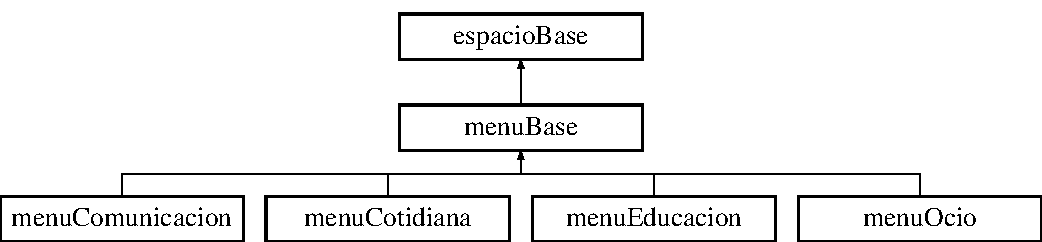
\includegraphics[height=3.000000cm]{classmenu_base}
\end{center}
\end{figure}
\subsection*{Métodos públicos}
\begin{DoxyCompactItemize}
\item 
\hyperlink{classmenu_base_a39dcbe65c2af659e4d27da0ec81f5824}{menu\+Base} (string, \hyperlink{classespacio_base}{espacio\+Base} $\ast$)
\begin{DoxyCompactList}\small\item\em Constructor de la clase. \end{DoxyCompactList}\item 
\hyperlink{classmenu_base_a09884cccdb9271476bbf6d87c6acfdfa}{$\sim$menu\+Base} ()
\begin{DoxyCompactList}\small\item\em Destructor de la clase. \end{DoxyCompactList}\item 
void \hyperlink{classmenu_base_a8d6e8078f62721431e095cb50bbcf40e}{setup} ()
\begin{DoxyCompactList}\small\item\em Método inicial del ciclo de Open\+G\+L. \end{DoxyCompactList}\item 
\hyperlink{classespacio_base}{espacio\+Base} $\ast$ \hyperlink{classmenu_base_aed2125585944e1dfa0ee7cb0e4f7958c}{update} (float, float, float, float, bool)
\begin{DoxyCompactList}\small\item\em Controla tareas lógica de cada ciclo de Open\+G\+L. \end{DoxyCompactList}\item 
void \hyperlink{classmenu_base_a0faf0816595b77204dd3e0309b35b76a}{draw} ()
\begin{DoxyCompactList}\small\item\em Controla las tareas gráficas de cada ciclo de Open\+G\+L. \end{DoxyCompactList}\end{DoxyCompactItemize}
\subsection*{Métodos protegidos}
\begin{DoxyCompactItemize}
\item 
virtual \hyperlink{classespacio_base}{espacio\+Base} $\ast$ \hyperlink{classmenu_base_a5a88a45efd3bc47b4731fb21749a97d5}{eventos} (int index)=0
\begin{DoxyCompactList}\small\item\em Maneja los eventos de los botones. \end{DoxyCompactList}\end{DoxyCompactItemize}
\subsection*{Atributos protegidos}
\begin{DoxyCompactItemize}
\item 
of\+True\+Type\+Font \hyperlink{classmenu_base_a8c48cc67dd9d789cf5a06c61333c8db9}{fuente}
\begin{DoxyCompactList}\small\item\em Fuente del texto. \end{DoxyCompactList}\item 
of\+Image \hyperlink{classmenu_base_a817536aa29cfe8f13d1e7c745e45b31d}{logo}
\begin{DoxyCompactList}\small\item\em Logo de la aplicación. \end{DoxyCompactList}\item 
float \hyperlink{classmenu_base_a97f2f1c174cadb12ae7b62f672fcde97}{logox}
\begin{DoxyCompactList}\small\item\em Coordenada x del logo. \end{DoxyCompactList}\item 
float \hyperlink{classmenu_base_a8bd56c156201d813c9c6da884cd98296}{logoy}
\begin{DoxyCompactList}\small\item\em Coordenada y del logo. \end{DoxyCompactList}\item 
ofx\+Xml\+Settings \hyperlink{classmenu_base_a07ca6fd4669759542b11d31eada55403}{configuraciones}
\begin{DoxyCompactList}\small\item\em Instancia que maneja las configuraciones desde un archivo X\+M\+L. \end{DoxyCompactList}\item 
vector$<$ \hyperlink{classboton_imagen}{boton\+Imagen} $>$ \hyperlink{classmenu_base_a6de979e3389d5918db62c75d886161d9}{btn}
\begin{DoxyCompactList}\small\item\em Botones que llevan al usuario a los espacios del menú \end{DoxyCompactList}\item 
\hyperlink{classboton_imagen}{boton\+Imagen} $\ast$ \hyperlink{classmenu_base_a28cf020839a96b7793388baf8a9e054d}{btn\+Atras}
\begin{DoxyCompactList}\small\item\em Botón para que el usuario se devuelva en la aplicación. \end{DoxyCompactList}\end{DoxyCompactItemize}


\subsection{Descripción detallada}
Base para los menús de la aplicación. 

Se pretende que los espacios de la aplicación se agrupen en categorías. Cada categoría tendrá su menú. Todos los menús heredan de esta clase para que se mantenga el mismo estilo. Cualquier cambio estético que se quisiera aplicar a todos los menús deberían integrarse acá.

Cada menú tiene su propio archivos de configuraciones. Este archivo tiene un formato X\+M\+L e indica los componentes que tendrá el menú. Además, los menús tienen las instancias de los espacios que están relacionados a su categoría. 

\subsection{Documentación del constructor y destructor}
\hypertarget{classmenu_base_a39dcbe65c2af659e4d27da0ec81f5824}{}\index{menu\+Base@{menu\+Base}!menu\+Base@{menu\+Base}}
\index{menu\+Base@{menu\+Base}!menu\+Base@{menu\+Base}}
\subsubsection[{menu\+Base(string, espacio\+Base $\ast$)}]{\setlength{\rightskip}{0pt plus 5cm}menu\+Base\+::menu\+Base (
\begin{DoxyParamCaption}
\item[{string}]{conf\+Path, }
\item[{{\bf espacio\+Base} $\ast$}]{esp\+Padre}
\end{DoxyParamCaption}
)}\label{classmenu_base_a39dcbe65c2af659e4d27da0ec81f5824}


Constructor de la clase. 

Carga el archivo de configuración.


\begin{DoxyParams}{Parámetros}
{\em conf\+Path} & Localización del archivo de configuración \\
\hline
{\em esp\+Padre} & Puntero al espacio/menú padre del menú \\
\hline
\end{DoxyParams}
\hypertarget{classmenu_base_a09884cccdb9271476bbf6d87c6acfdfa}{}\index{menu\+Base@{menu\+Base}!````~menu\+Base@{$\sim$menu\+Base}}
\index{````~menu\+Base@{$\sim$menu\+Base}!menu\+Base@{menu\+Base}}
\subsubsection[{$\sim$menu\+Base()}]{\setlength{\rightskip}{0pt plus 5cm}menu\+Base\+::$\sim$menu\+Base (
\begin{DoxyParamCaption}
{}
\end{DoxyParamCaption}
)}\label{classmenu_base_a09884cccdb9271476bbf6d87c6acfdfa}


Destructor de la clase. 



\subsection{Documentación de las funciones miembro}
\hypertarget{classmenu_base_a0faf0816595b77204dd3e0309b35b76a}{}\index{menu\+Base@{menu\+Base}!draw@{draw}}
\index{draw@{draw}!menu\+Base@{menu\+Base}}
\subsubsection[{draw()}]{\setlength{\rightskip}{0pt plus 5cm}void menu\+Base\+::draw (
\begin{DoxyParamCaption}
{}
\end{DoxyParamCaption}
)\hspace{0.3cm}{\ttfamily [virtual]}}\label{classmenu_base_a0faf0816595b77204dd3e0309b35b76a}


Controla las tareas gráficas de cada ciclo de Open\+G\+L. 



Implementa \hyperlink{classespacio_base_a01b3e668211b6159784f79a3f5a32d95}{espacio\+Base}.

\hypertarget{classmenu_base_a5a88a45efd3bc47b4731fb21749a97d5}{}\index{menu\+Base@{menu\+Base}!eventos@{eventos}}
\index{eventos@{eventos}!menu\+Base@{menu\+Base}}
\subsubsection[{eventos(int index)=0}]{\setlength{\rightskip}{0pt plus 5cm}virtual {\bf espacio\+Base}$\ast$ menu\+Base\+::eventos (
\begin{DoxyParamCaption}
\item[{int}]{index}
\end{DoxyParamCaption}
)\hspace{0.3cm}{\ttfamily [protected]}, {\ttfamily [pure virtual]}}\label{classmenu_base_a5a88a45efd3bc47b4731fb21749a97d5}


Maneja los eventos de los botones. 

Cada menú tiene una cantidad determinada de botones. Para cada uno de ellos se implementa un evento que se dispara cuando el usuario hace clic


\begin{DoxyParams}{Parámetros}
{\em index} & Indice del boton en la lista btn \\
\hline
\end{DoxyParams}


Implementado en \hyperlink{classmenu_comunicacion_a7386759ca2897f5ce031bf4c166fa8a1}{menu\+Comunicacion}, \hyperlink{classmenu_ocio_ab64d85113d3df4d1ba3b7599b89d0598}{menu\+Ocio}, \hyperlink{classmenu_educacion_af29464c6a5f1bb3c57ac6e12d3fcc740}{menu\+Educacion} y \hyperlink{classmenu_cotidiana_a5bc0b717e3cf19d4daa8bb73f3669f3a}{menu\+Cotidiana}.

\hypertarget{classmenu_base_a8d6e8078f62721431e095cb50bbcf40e}{}\index{menu\+Base@{menu\+Base}!setup@{setup}}
\index{setup@{setup}!menu\+Base@{menu\+Base}}
\subsubsection[{setup()}]{\setlength{\rightskip}{0pt plus 5cm}void menu\+Base\+::setup (
\begin{DoxyParamCaption}
{}
\end{DoxyParamCaption}
)\hspace{0.3cm}{\ttfamily [virtual]}}\label{classmenu_base_a8d6e8078f62721431e095cb50bbcf40e}


Método inicial del ciclo de Open\+G\+L. 



Implementa \hyperlink{classespacio_base_a65020ad1e767a235b0c227a1769c5416}{espacio\+Base}.



Reimplementado en \hyperlink{classmenu_comunicacion_a9e42e30977954e20c304261a9f1be5e1}{menu\+Comunicacion}, \hyperlink{classmenu_ocio_a6b99292a5b8c60b5a8a799447fc85f18}{menu\+Ocio} y \hyperlink{classmenu_educacion_a782815ae0152a27aca5d33885f607e81}{menu\+Educacion}.

\hypertarget{classmenu_base_aed2125585944e1dfa0ee7cb0e4f7958c}{}\index{menu\+Base@{menu\+Base}!update@{update}}
\index{update@{update}!menu\+Base@{menu\+Base}}
\subsubsection[{update(float, float, float, float, bool)}]{\setlength{\rightskip}{0pt plus 5cm}{\bf espacio\+Base} $\ast$ menu\+Base\+::update (
\begin{DoxyParamCaption}
\item[{float}]{, }
\item[{float}]{, }
\item[{float}]{, }
\item[{float}]{, }
\item[{bool}]{}
\end{DoxyParamCaption}
)\hspace{0.3cm}{\ttfamily [virtual]}}\label{classmenu_base_aed2125585944e1dfa0ee7cb0e4f7958c}


Controla tareas lógica de cada ciclo de Open\+G\+L. 



Implementa \hyperlink{classespacio_base_a9b94b1106cd478dd78bc42078a36d013}{espacio\+Base}.



\subsection{Documentación de los datos miembro}
\hypertarget{classmenu_base_a6de979e3389d5918db62c75d886161d9}{}\index{menu\+Base@{menu\+Base}!btn@{btn}}
\index{btn@{btn}!menu\+Base@{menu\+Base}}
\subsubsection[{btn}]{\setlength{\rightskip}{0pt plus 5cm}vector$<${\bf boton\+Imagen}$>$ menu\+Base\+::btn\hspace{0.3cm}{\ttfamily [protected]}}\label{classmenu_base_a6de979e3389d5918db62c75d886161d9}


Botones que llevan al usuario a los espacios del menú 

\hypertarget{classmenu_base_a28cf020839a96b7793388baf8a9e054d}{}\index{menu\+Base@{menu\+Base}!btn\+Atras@{btn\+Atras}}
\index{btn\+Atras@{btn\+Atras}!menu\+Base@{menu\+Base}}
\subsubsection[{btn\+Atras}]{\setlength{\rightskip}{0pt plus 5cm}{\bf boton\+Imagen}$\ast$ menu\+Base\+::btn\+Atras\hspace{0.3cm}{\ttfamily [protected]}}\label{classmenu_base_a28cf020839a96b7793388baf8a9e054d}


Botón para que el usuario se devuelva en la aplicación. 

\hypertarget{classmenu_base_a07ca6fd4669759542b11d31eada55403}{}\index{menu\+Base@{menu\+Base}!configuraciones@{configuraciones}}
\index{configuraciones@{configuraciones}!menu\+Base@{menu\+Base}}
\subsubsection[{configuraciones}]{\setlength{\rightskip}{0pt plus 5cm}ofx\+Xml\+Settings menu\+Base\+::configuraciones\hspace{0.3cm}{\ttfamily [protected]}}\label{classmenu_base_a07ca6fd4669759542b11d31eada55403}


Instancia que maneja las configuraciones desde un archivo X\+M\+L. 

\hypertarget{classmenu_base_a8c48cc67dd9d789cf5a06c61333c8db9}{}\index{menu\+Base@{menu\+Base}!fuente@{fuente}}
\index{fuente@{fuente}!menu\+Base@{menu\+Base}}
\subsubsection[{fuente}]{\setlength{\rightskip}{0pt plus 5cm}of\+True\+Type\+Font menu\+Base\+::fuente\hspace{0.3cm}{\ttfamily [protected]}}\label{classmenu_base_a8c48cc67dd9d789cf5a06c61333c8db9}


Fuente del texto. 

\hypertarget{classmenu_base_a817536aa29cfe8f13d1e7c745e45b31d}{}\index{menu\+Base@{menu\+Base}!logo@{logo}}
\index{logo@{logo}!menu\+Base@{menu\+Base}}
\subsubsection[{logo}]{\setlength{\rightskip}{0pt plus 5cm}of\+Image menu\+Base\+::logo\hspace{0.3cm}{\ttfamily [protected]}}\label{classmenu_base_a817536aa29cfe8f13d1e7c745e45b31d}


Logo de la aplicación. 

\hypertarget{classmenu_base_a97f2f1c174cadb12ae7b62f672fcde97}{}\index{menu\+Base@{menu\+Base}!logox@{logox}}
\index{logox@{logox}!menu\+Base@{menu\+Base}}
\subsubsection[{logox}]{\setlength{\rightskip}{0pt plus 5cm}float menu\+Base\+::logox\hspace{0.3cm}{\ttfamily [protected]}}\label{classmenu_base_a97f2f1c174cadb12ae7b62f672fcde97}


Coordenada x del logo. 

\hypertarget{classmenu_base_a8bd56c156201d813c9c6da884cd98296}{}\index{menu\+Base@{menu\+Base}!logoy@{logoy}}
\index{logoy@{logoy}!menu\+Base@{menu\+Base}}
\subsubsection[{logoy}]{\setlength{\rightskip}{0pt plus 5cm}float menu\+Base\+::logoy\hspace{0.3cm}{\ttfamily [protected]}}\label{classmenu_base_a8bd56c156201d813c9c6da884cd98296}


Coordenada y del logo. 



La documentación para esta clase fue generada a partir de los siguientes ficheros\+:\begin{DoxyCompactItemize}
\item 
C\+:/of\+\_\+v0.\+8.\+4\+\_\+vs\+\_\+release/apps/my\+Apps/\+Robo\+Tracking\+App/src/menus/\hyperlink{menu_base_8h}{menu\+Base.\+h}\item 
C\+:/of\+\_\+v0.\+8.\+4\+\_\+vs\+\_\+release/apps/my\+Apps/\+Robo\+Tracking\+App/src/menus/\hyperlink{menu_base_8cpp}{menu\+Base.\+cpp}\end{DoxyCompactItemize}

\hypertarget{classmenu_comunicacion}{}\section{Referencia de la Clase menu\+Comunicacion}
\label{classmenu_comunicacion}\index{menu\+Comunicacion@{menu\+Comunicacion}}


Menú de la categoría comunicación.  




{\ttfamily \#include $<$menu\+Comunicacion.\+h$>$}

Diagrama de herencias de menu\+Comunicacion\begin{figure}[H]
\begin{center}
\leavevmode
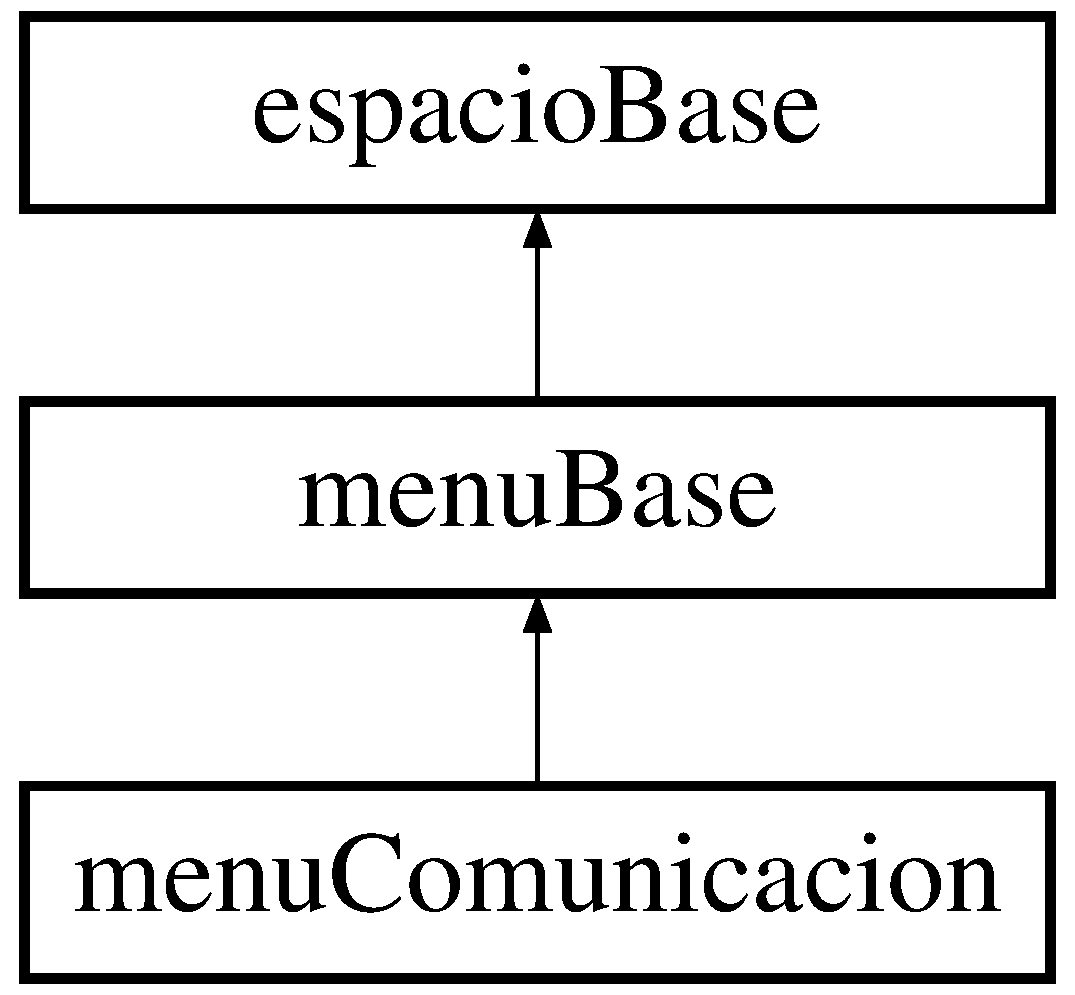
\includegraphics[height=3.000000cm]{classmenu_comunicacion}
\end{center}
\end{figure}
\subsection*{Métodos públicos}
\begin{DoxyCompactItemize}
\item 
\hyperlink{classmenu_comunicacion_a9a96fdc1109e1b41e4928f35833cd445}{menu\+Comunicacion} (\hyperlink{classespacio_base}{espacio\+Base} $\ast$m\+Padre)
\begin{DoxyCompactList}\small\item\em Constructor de la clase. \end{DoxyCompactList}\item 
\hyperlink{classmenu_comunicacion_a16b316cb60f2a95ae40bdc1a7fe26777}{$\sim$menu\+Comunicacion} ()
\begin{DoxyCompactList}\small\item\em Destructor de la clase. \end{DoxyCompactList}\item 
void \hyperlink{classmenu_comunicacion_a9e42e30977954e20c304261a9f1be5e1}{setup} ()
\begin{DoxyCompactList}\small\item\em Método inicial del ciclo de Open\+G\+L. \end{DoxyCompactList}\end{DoxyCompactItemize}
\subsection*{Métodos privados}
\begin{DoxyCompactItemize}
\item 
\hyperlink{classespacio_base}{espacio\+Base} $\ast$ \hyperlink{classmenu_comunicacion_a7386759ca2897f5ce031bf4c166fa8a1}{eventos} (int)
\begin{DoxyCompactList}\small\item\em Maneja los eventos de los botones. \end{DoxyCompactList}\end{DoxyCompactItemize}
\subsection*{Atributos privados}
\begin{DoxyCompactItemize}
\item 
\hyperlink{classespacio_teclado}{espacio\+Teclado} $\ast$ \hyperlink{classmenu_comunicacion_a01b499ef3e349868508abfd4f856bbea}{esp\+Teclado}
\begin{DoxyCompactList}\small\item\em Instancia del espacio teclado. \end{DoxyCompactList}\item 
\hyperlink{classespacio_pictograma}{espacio\+Pictograma} $\ast$ \hyperlink{classmenu_comunicacion_ac00c26aae43f331167e102e2b6d7b86c}{esp\+Pictograma}
\begin{DoxyCompactList}\small\item\em Instancia del espacio pictogramas. \end{DoxyCompactList}\item 
\hyperlink{classespacio_si_no}{espacio\+Si\+No} $\ast$ \hyperlink{classmenu_comunicacion_ab9fc64713344f895347473d97f555a8e}{esp\+Si\+No}
\begin{DoxyCompactList}\small\item\em Instancia del espacio si/no. \end{DoxyCompactList}\end{DoxyCompactItemize}
\subsection*{Otros miembros heredados}


\subsection{Descripción detallada}
Menú de la categoría comunicación. 

\subsection{Documentación del constructor y destructor}
\hypertarget{classmenu_comunicacion_a9a96fdc1109e1b41e4928f35833cd445}{}\index{menu\+Comunicacion@{menu\+Comunicacion}!menu\+Comunicacion@{menu\+Comunicacion}}
\index{menu\+Comunicacion@{menu\+Comunicacion}!menu\+Comunicacion@{menu\+Comunicacion}}
\subsubsection[{menu\+Comunicacion(espacio\+Base $\ast$m\+Padre)}]{\setlength{\rightskip}{0pt plus 5cm}menu\+Comunicacion\+::menu\+Comunicacion (
\begin{DoxyParamCaption}
\item[{{\bf espacio\+Base} $\ast$}]{m\+Padre}
\end{DoxyParamCaption}
)\hspace{0.3cm}{\ttfamily [inline]}}\label{classmenu_comunicacion_a9a96fdc1109e1b41e4928f35833cd445}


Constructor de la clase. 


\begin{DoxyParams}{Parámetros}
{\em m\+Padre} & puntero al menú principal \\
\hline
\end{DoxyParams}
\hypertarget{classmenu_comunicacion_a16b316cb60f2a95ae40bdc1a7fe26777}{}\index{menu\+Comunicacion@{menu\+Comunicacion}!````~menu\+Comunicacion@{$\sim$menu\+Comunicacion}}
\index{````~menu\+Comunicacion@{$\sim$menu\+Comunicacion}!menu\+Comunicacion@{menu\+Comunicacion}}
\subsubsection[{$\sim$menu\+Comunicacion()}]{\setlength{\rightskip}{0pt plus 5cm}menu\+Comunicacion\+::$\sim$menu\+Comunicacion (
\begin{DoxyParamCaption}
{}
\end{DoxyParamCaption}
)}\label{classmenu_comunicacion_a16b316cb60f2a95ae40bdc1a7fe26777}


Destructor de la clase. 



\subsection{Documentación de las funciones miembro}
\hypertarget{classmenu_comunicacion_a7386759ca2897f5ce031bf4c166fa8a1}{}\index{menu\+Comunicacion@{menu\+Comunicacion}!eventos@{eventos}}
\index{eventos@{eventos}!menu\+Comunicacion@{menu\+Comunicacion}}
\subsubsection[{eventos(int)}]{\setlength{\rightskip}{0pt plus 5cm}{\bf espacio\+Base} $\ast$ menu\+Comunicacion\+::eventos (
\begin{DoxyParamCaption}
\item[{int}]{index}
\end{DoxyParamCaption}
)\hspace{0.3cm}{\ttfamily [private]}, {\ttfamily [virtual]}}\label{classmenu_comunicacion_a7386759ca2897f5ce031bf4c166fa8a1}


Maneja los eventos de los botones. 

Cada menú tiene una cantidad determinada de botones. Para cada uno de ellos se implementa un evento que se dispara cuando el usuario hace clic


\begin{DoxyParams}{Parámetros}
{\em index} & Indice del boton en la lista btn \\
\hline
\end{DoxyParams}


Implementa \hyperlink{classmenu_base_a5a88a45efd3bc47b4731fb21749a97d5}{menu\+Base}.

\hypertarget{classmenu_comunicacion_a9e42e30977954e20c304261a9f1be5e1}{}\index{menu\+Comunicacion@{menu\+Comunicacion}!setup@{setup}}
\index{setup@{setup}!menu\+Comunicacion@{menu\+Comunicacion}}
\subsubsection[{setup()}]{\setlength{\rightskip}{0pt plus 5cm}void menu\+Comunicacion\+::setup (
\begin{DoxyParamCaption}
{}
\end{DoxyParamCaption}
)\hspace{0.3cm}{\ttfamily [virtual]}}\label{classmenu_comunicacion_a9e42e30977954e20c304261a9f1be5e1}


Método inicial del ciclo de Open\+G\+L. 



Reimplementado de \hyperlink{classmenu_base_a8d6e8078f62721431e095cb50bbcf40e}{menu\+Base}.



\subsection{Documentación de los datos miembro}
\hypertarget{classmenu_comunicacion_ac00c26aae43f331167e102e2b6d7b86c}{}\index{menu\+Comunicacion@{menu\+Comunicacion}!esp\+Pictograma@{esp\+Pictograma}}
\index{esp\+Pictograma@{esp\+Pictograma}!menu\+Comunicacion@{menu\+Comunicacion}}
\subsubsection[{esp\+Pictograma}]{\setlength{\rightskip}{0pt plus 5cm}{\bf espacio\+Pictograma}$\ast$ menu\+Comunicacion\+::esp\+Pictograma\hspace{0.3cm}{\ttfamily [private]}}\label{classmenu_comunicacion_ac00c26aae43f331167e102e2b6d7b86c}


Instancia del espacio pictogramas. 

\hypertarget{classmenu_comunicacion_ab9fc64713344f895347473d97f555a8e}{}\index{menu\+Comunicacion@{menu\+Comunicacion}!esp\+Si\+No@{esp\+Si\+No}}
\index{esp\+Si\+No@{esp\+Si\+No}!menu\+Comunicacion@{menu\+Comunicacion}}
\subsubsection[{esp\+Si\+No}]{\setlength{\rightskip}{0pt plus 5cm}{\bf espacio\+Si\+No}$\ast$ menu\+Comunicacion\+::esp\+Si\+No\hspace{0.3cm}{\ttfamily [private]}}\label{classmenu_comunicacion_ab9fc64713344f895347473d97f555a8e}


Instancia del espacio si/no. 

\hypertarget{classmenu_comunicacion_a01b499ef3e349868508abfd4f856bbea}{}\index{menu\+Comunicacion@{menu\+Comunicacion}!esp\+Teclado@{esp\+Teclado}}
\index{esp\+Teclado@{esp\+Teclado}!menu\+Comunicacion@{menu\+Comunicacion}}
\subsubsection[{esp\+Teclado}]{\setlength{\rightskip}{0pt plus 5cm}{\bf espacio\+Teclado}$\ast$ menu\+Comunicacion\+::esp\+Teclado\hspace{0.3cm}{\ttfamily [private]}}\label{classmenu_comunicacion_a01b499ef3e349868508abfd4f856bbea}


Instancia del espacio teclado. 



La documentación para esta clase fue generada a partir de los siguientes ficheros\+:\begin{DoxyCompactItemize}
\item 
C\+:/of\+\_\+v0.\+8.\+4\+\_\+vs\+\_\+release/apps/my\+Apps/\+Robo\+Tracking\+App/src/menus/\hyperlink{menu_comunicacion_8h}{menu\+Comunicacion.\+h}\item 
C\+:/of\+\_\+v0.\+8.\+4\+\_\+vs\+\_\+release/apps/my\+Apps/\+Robo\+Tracking\+App/src/menus/\hyperlink{menu_comunicacion_8cpp}{menu\+Comunicacion.\+cpp}\end{DoxyCompactItemize}

\hypertarget{classmenu_cotidiana}{}\section{Referencia de la Clase menu\+Cotidiana}
\label{classmenu_cotidiana}\index{menu\+Cotidiana@{menu\+Cotidiana}}


Menú de la categoría vida cotidiana.  




{\ttfamily \#include $<$menu\+Cotidiana.\+h$>$}

Diagrama de herencias de menu\+Cotidiana\begin{figure}[H]
\begin{center}
\leavevmode
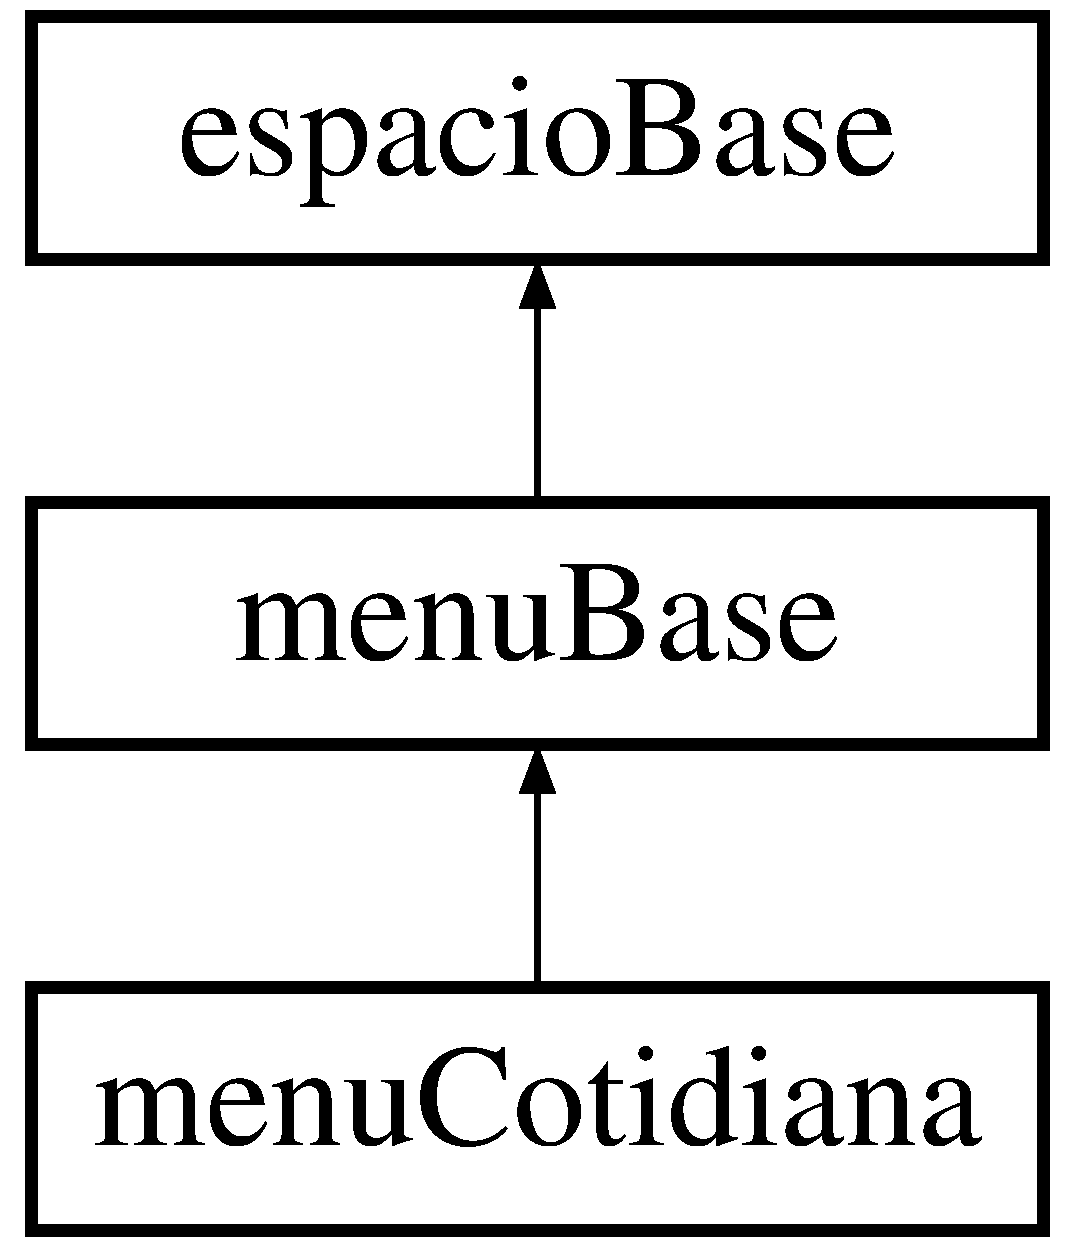
\includegraphics[height=3.000000cm]{classmenu_cotidiana}
\end{center}
\end{figure}
\subsection*{Métodos públicos}
\begin{DoxyCompactItemize}
\item 
\hyperlink{classmenu_cotidiana_a7af3789d7f16fec560bf7c5723b38581}{menu\+Cotidiana} (\hyperlink{classespacio_base}{espacio\+Base} $\ast$m\+Padre)
\begin{DoxyCompactList}\small\item\em Constructor de la clase. \end{DoxyCompactList}\end{DoxyCompactItemize}
\subsection*{Métodos protegidos}
\begin{DoxyCompactItemize}
\item 
\hyperlink{classespacio_base}{espacio\+Base} $\ast$ \hyperlink{classmenu_cotidiana_a5bc0b717e3cf19d4daa8bb73f3669f3a}{eventos} (int)
\begin{DoxyCompactList}\small\item\em Maneja los eventos de los botones. \end{DoxyCompactList}\end{DoxyCompactItemize}
\subsection*{Otros miembros heredados}


\subsection{Descripción detallada}
Menú de la categoría vida cotidiana. 

\subsection{Documentación del constructor y destructor}
\hypertarget{classmenu_cotidiana_a7af3789d7f16fec560bf7c5723b38581}{}\index{menu\+Cotidiana@{menu\+Cotidiana}!menu\+Cotidiana@{menu\+Cotidiana}}
\index{menu\+Cotidiana@{menu\+Cotidiana}!menu\+Cotidiana@{menu\+Cotidiana}}
\subsubsection[{menu\+Cotidiana(espacio\+Base $\ast$m\+Padre)}]{\setlength{\rightskip}{0pt plus 5cm}menu\+Cotidiana\+::menu\+Cotidiana (
\begin{DoxyParamCaption}
\item[{{\bf espacio\+Base} $\ast$}]{m\+Padre}
\end{DoxyParamCaption}
)\hspace{0.3cm}{\ttfamily [inline]}}\label{classmenu_cotidiana_a7af3789d7f16fec560bf7c5723b38581}


Constructor de la clase. 


\begin{DoxyParams}{Parámetros}
{\em m\+Padre} & puntero al menú principal \\
\hline
\end{DoxyParams}


\subsection{Documentación de las funciones miembro}
\hypertarget{classmenu_cotidiana_a5bc0b717e3cf19d4daa8bb73f3669f3a}{}\index{menu\+Cotidiana@{menu\+Cotidiana}!eventos@{eventos}}
\index{eventos@{eventos}!menu\+Cotidiana@{menu\+Cotidiana}}
\subsubsection[{eventos(int)}]{\setlength{\rightskip}{0pt plus 5cm}{\bf espacio\+Base} $\ast$ menu\+Cotidiana\+::eventos (
\begin{DoxyParamCaption}
\item[{int}]{index}
\end{DoxyParamCaption}
)\hspace{0.3cm}{\ttfamily [protected]}, {\ttfamily [virtual]}}\label{classmenu_cotidiana_a5bc0b717e3cf19d4daa8bb73f3669f3a}


Maneja los eventos de los botones. 

Cada menú tiene una cantidad determinada de botones. Para cada uno de ellos se implementa un evento que se dispara cuando el usuario hace clic


\begin{DoxyParams}{Parámetros}
{\em index} & Indice del boton en la lista btn \\
\hline
\end{DoxyParams}


Implementa \hyperlink{classmenu_base_a5a88a45efd3bc47b4731fb21749a97d5}{menu\+Base}.



La documentación para esta clase fue generada a partir de los siguientes ficheros\+:\begin{DoxyCompactItemize}
\item 
C\+:/of\+\_\+v0.\+8.\+4\+\_\+vs\+\_\+release/apps/my\+Apps/\+Robo\+Tracking\+App/src/menus/\hyperlink{menu_cotidiana_8h}{menu\+Cotidiana.\+h}\item 
C\+:/of\+\_\+v0.\+8.\+4\+\_\+vs\+\_\+release/apps/my\+Apps/\+Robo\+Tracking\+App/src/menus/\hyperlink{menu_cotidiana_8cpp}{menu\+Cotidiana.\+cpp}\end{DoxyCompactItemize}

\hypertarget{classmenu_educacion}{}\section{Referencia de la Clase menu\+Educacion}
\label{classmenu_educacion}\index{menu\+Educacion@{menu\+Educacion}}


Menú de la categoría educación.  




{\ttfamily \#include $<$menu\+Educacion.\+h$>$}

Diagrama de herencias de menu\+Educacion\begin{figure}[H]
\begin{center}
\leavevmode
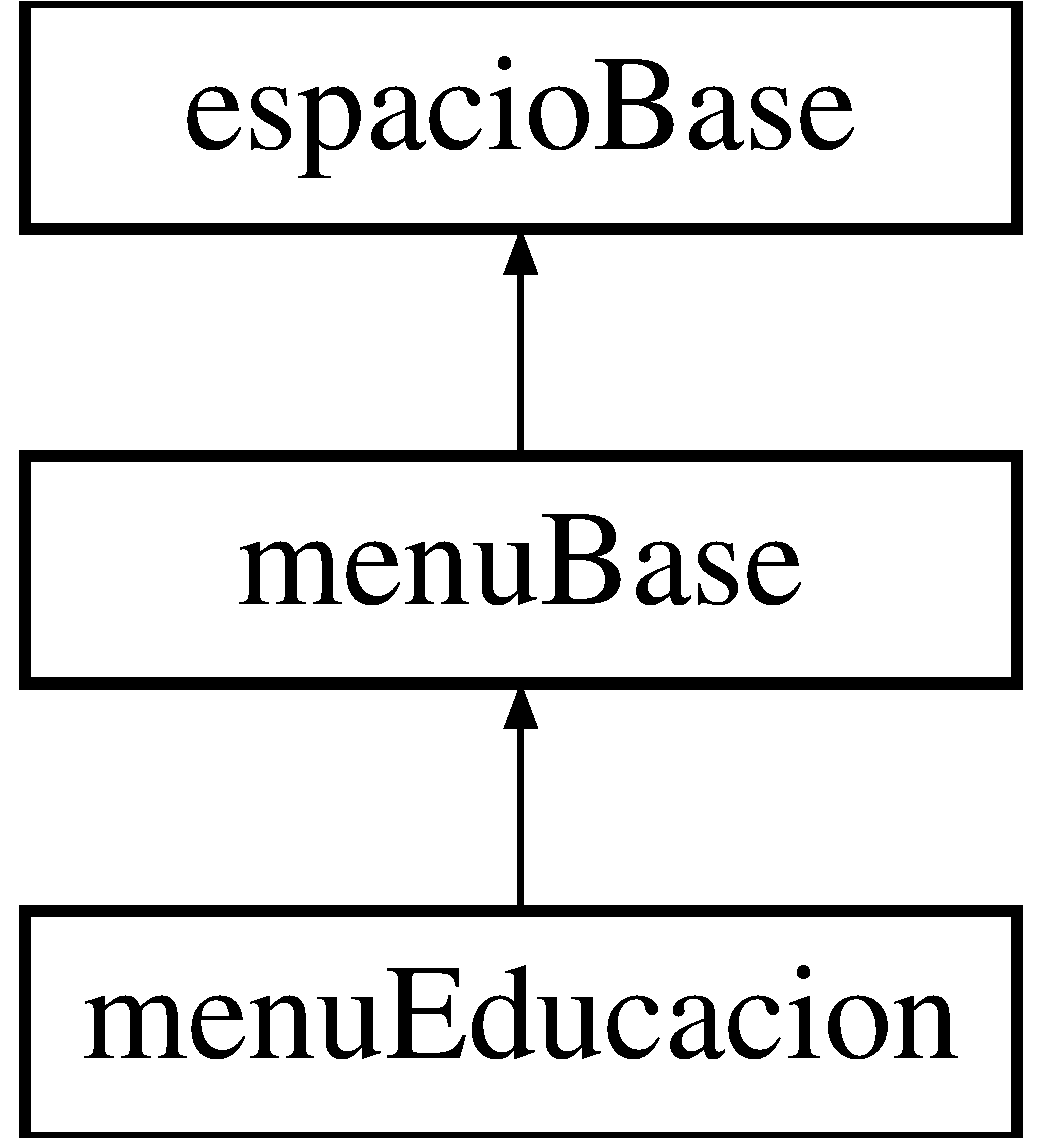
\includegraphics[height=3.000000cm]{classmenu_educacion}
\end{center}
\end{figure}
\subsection*{Métodos públicos}
\begin{DoxyCompactItemize}
\item 
\hyperlink{classmenu_educacion_a2fba0b83189f92ad20f6fc2526c5ba6f}{menu\+Educacion} (\hyperlink{classespacio_base}{espacio\+Base} $\ast$m\+Padre)
\begin{DoxyCompactList}\small\item\em Constructor de la clase. \end{DoxyCompactList}\item 
\hyperlink{classmenu_educacion_a5613fcc80f443081cadc8a1bfb1c8b97}{$\sim$menu\+Educacion} ()
\begin{DoxyCompactList}\small\item\em Destructor de la clase. \end{DoxyCompactList}\item 
void \hyperlink{classmenu_educacion_a782815ae0152a27aca5d33885f607e81}{setup} ()
\begin{DoxyCompactList}\small\item\em Método inicial del ciclo de Open\+G\+L. \end{DoxyCompactList}\end{DoxyCompactItemize}
\subsection*{Métodos protegidos}
\begin{DoxyCompactItemize}
\item 
\hyperlink{classespacio_base}{espacio\+Base} $\ast$ \hyperlink{classmenu_educacion_af29464c6a5f1bb3c57ac6e12d3fcc740}{eventos} (int)
\begin{DoxyCompactList}\small\item\em Maneja los eventos de los botones. \end{DoxyCompactList}\end{DoxyCompactItemize}
\subsection*{Atributos protegidos}
\begin{DoxyCompactItemize}
\item 
\hyperlink{classespacio_tarjetas}{espacio\+Tarjetas} $\ast$ \hyperlink{classmenu_educacion_a602af7d2ec9b39832ff788282b43e4af}{tarjetas}
\begin{DoxyCompactList}\small\item\em Instancia del espacio tarjetas. \end{DoxyCompactList}\end{DoxyCompactItemize}


\subsection{Descripción detallada}
Menú de la categoría educación. 

\subsection{Documentación del constructor y destructor}
\hypertarget{classmenu_educacion_a2fba0b83189f92ad20f6fc2526c5ba6f}{}\index{menu\+Educacion@{menu\+Educacion}!menu\+Educacion@{menu\+Educacion}}
\index{menu\+Educacion@{menu\+Educacion}!menu\+Educacion@{menu\+Educacion}}
\subsubsection[{menu\+Educacion(espacio\+Base $\ast$m\+Padre)}]{\setlength{\rightskip}{0pt plus 5cm}menu\+Educacion\+::menu\+Educacion (
\begin{DoxyParamCaption}
\item[{{\bf espacio\+Base} $\ast$}]{m\+Padre}
\end{DoxyParamCaption}
)\hspace{0.3cm}{\ttfamily [inline]}}\label{classmenu_educacion_a2fba0b83189f92ad20f6fc2526c5ba6f}


Constructor de la clase. 


\begin{DoxyParams}{Parámetros}
{\em m\+Padre} & puntero al menú principal \\
\hline
\end{DoxyParams}
\hypertarget{classmenu_educacion_a5613fcc80f443081cadc8a1bfb1c8b97}{}\index{menu\+Educacion@{menu\+Educacion}!````~menu\+Educacion@{$\sim$menu\+Educacion}}
\index{````~menu\+Educacion@{$\sim$menu\+Educacion}!menu\+Educacion@{menu\+Educacion}}
\subsubsection[{$\sim$menu\+Educacion()}]{\setlength{\rightskip}{0pt plus 5cm}menu\+Educacion\+::$\sim$menu\+Educacion (
\begin{DoxyParamCaption}
{}
\end{DoxyParamCaption}
)}\label{classmenu_educacion_a5613fcc80f443081cadc8a1bfb1c8b97}


Destructor de la clase. 



\subsection{Documentación de las funciones miembro}
\hypertarget{classmenu_educacion_af29464c6a5f1bb3c57ac6e12d3fcc740}{}\index{menu\+Educacion@{menu\+Educacion}!eventos@{eventos}}
\index{eventos@{eventos}!menu\+Educacion@{menu\+Educacion}}
\subsubsection[{eventos(int)}]{\setlength{\rightskip}{0pt plus 5cm}{\bf espacio\+Base} $\ast$ menu\+Educacion\+::eventos (
\begin{DoxyParamCaption}
\item[{int}]{index}
\end{DoxyParamCaption}
)\hspace{0.3cm}{\ttfamily [protected]}, {\ttfamily [virtual]}}\label{classmenu_educacion_af29464c6a5f1bb3c57ac6e12d3fcc740}


Maneja los eventos de los botones. 

Cada menú tiene una cantidad determinada de botones. Para cada uno de ellos se implementa un evento que se dispara cuando el usuario hace clic


\begin{DoxyParams}{Parámetros}
{\em index} & Indice del boton en la lista btn \\
\hline
\end{DoxyParams}


Implementa \hyperlink{classmenu_base_a5a88a45efd3bc47b4731fb21749a97d5}{menu\+Base}.

\hypertarget{classmenu_educacion_a782815ae0152a27aca5d33885f607e81}{}\index{menu\+Educacion@{menu\+Educacion}!setup@{setup}}
\index{setup@{setup}!menu\+Educacion@{menu\+Educacion}}
\subsubsection[{setup()}]{\setlength{\rightskip}{0pt plus 5cm}void menu\+Educacion\+::setup (
\begin{DoxyParamCaption}
{}
\end{DoxyParamCaption}
)\hspace{0.3cm}{\ttfamily [virtual]}}\label{classmenu_educacion_a782815ae0152a27aca5d33885f607e81}


Método inicial del ciclo de Open\+G\+L. 



Reimplementado de \hyperlink{classmenu_base_a8d6e8078f62721431e095cb50bbcf40e}{menu\+Base}.



\subsection{Documentación de los datos miembro}
\hypertarget{classmenu_educacion_a602af7d2ec9b39832ff788282b43e4af}{}\index{menu\+Educacion@{menu\+Educacion}!tarjetas@{tarjetas}}
\index{tarjetas@{tarjetas}!menu\+Educacion@{menu\+Educacion}}
\subsubsection[{tarjetas}]{\setlength{\rightskip}{0pt plus 5cm}{\bf espacio\+Tarjetas}$\ast$ menu\+Educacion\+::tarjetas\hspace{0.3cm}{\ttfamily [protected]}}\label{classmenu_educacion_a602af7d2ec9b39832ff788282b43e4af}


Instancia del espacio tarjetas. 



La documentación para esta clase fue generada a partir de los siguientes ficheros\+:\begin{DoxyCompactItemize}
\item 
C\+:/of\+\_\+v0.\+8.\+4\+\_\+vs\+\_\+release/apps/my\+Apps/\+Robo\+Tracking\+App/src/menus/\hyperlink{menu_educacion_8h}{menu\+Educacion.\+h}\item 
C\+:/of\+\_\+v0.\+8.\+4\+\_\+vs\+\_\+release/apps/my\+Apps/\+Robo\+Tracking\+App/src/menus/\hyperlink{menu_educacion_8cpp}{menu\+Educacion.\+cpp}\end{DoxyCompactItemize}

\hypertarget{classmenu_ocio}{}\section{Referencia de la Clase menu\+Ocio}
\label{classmenu_ocio}\index{menu\+Ocio@{menu\+Ocio}}


Menú de la categoría ocio.  




{\ttfamily \#include $<$menu\+Ocio.\+h$>$}

Diagrama de herencias de menu\+Ocio\begin{figure}[H]
\begin{center}
\leavevmode
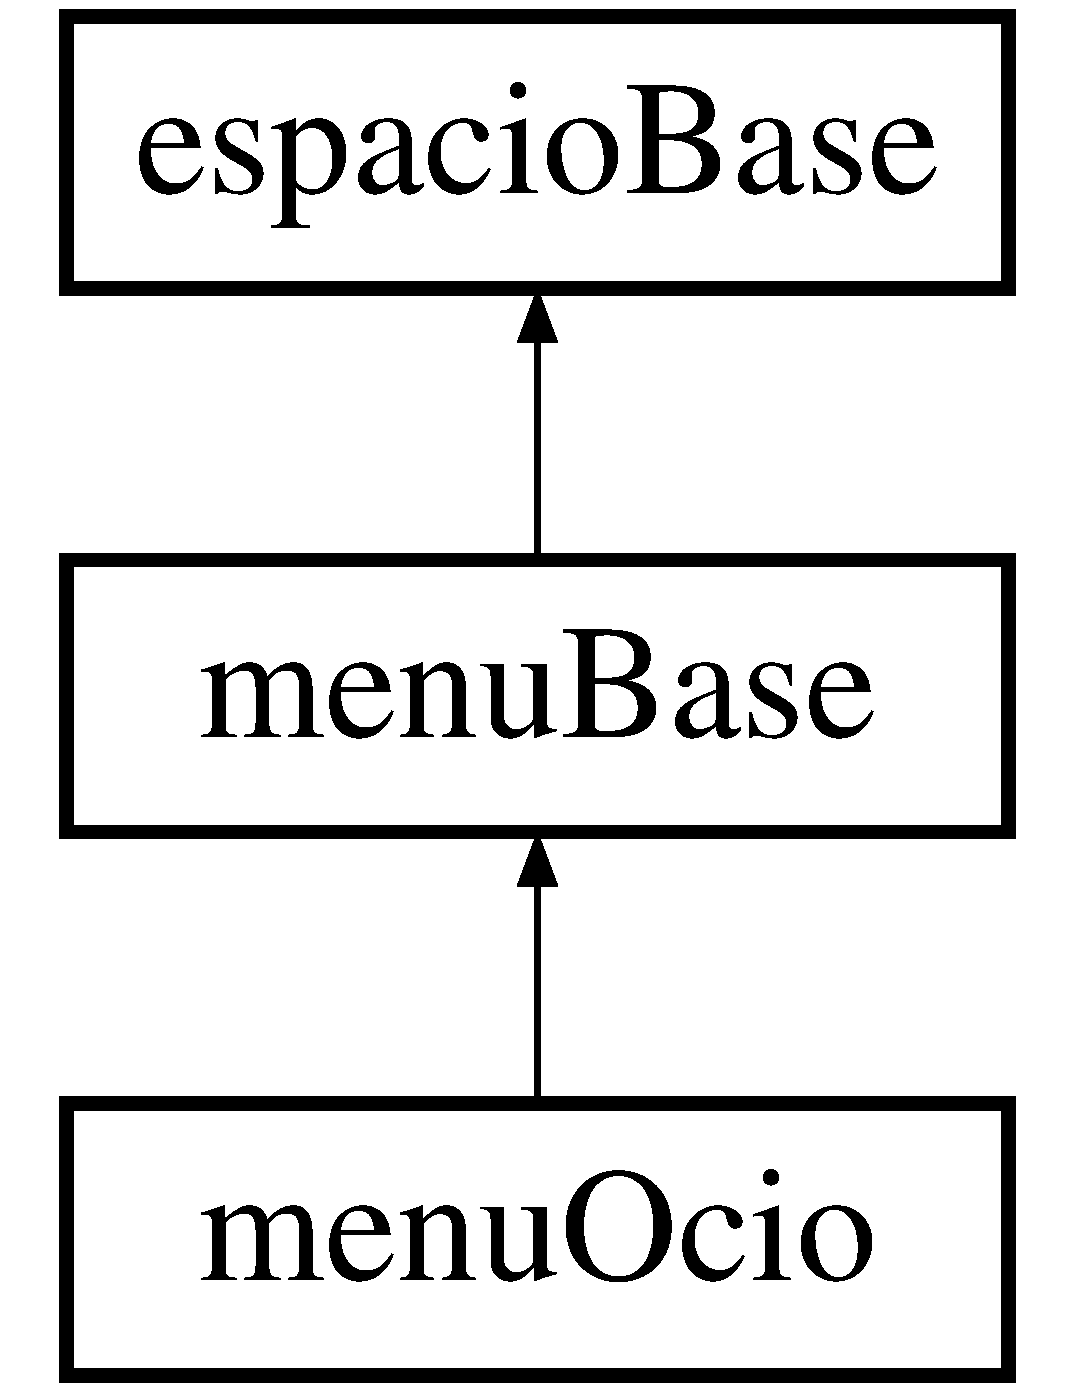
\includegraphics[height=3.000000cm]{classmenu_ocio}
\end{center}
\end{figure}
\subsection*{Métodos públicos}
\begin{DoxyCompactItemize}
\item 
\hyperlink{classmenu_ocio_a8da970ed63504b0071f9ba0472ef74d5}{menu\+Ocio} (\hyperlink{classespacio_base}{espacio\+Base} $\ast$)
\begin{DoxyCompactList}\small\item\em Constructor de la clase. \end{DoxyCompactList}\item 
\hyperlink{classmenu_ocio_ab0efb299b639818adafec4d91fd83c9e}{$\sim$menu\+Ocio} ()
\begin{DoxyCompactList}\small\item\em Destructor de la clase. \end{DoxyCompactList}\item 
void \hyperlink{classmenu_ocio_a6b99292a5b8c60b5a8a799447fc85f18}{setup} ()
\begin{DoxyCompactList}\small\item\em Método inicial del ciclo de Open\+G\+L. \end{DoxyCompactList}\end{DoxyCompactItemize}
\subsection*{Métodos protegidos}
\begin{DoxyCompactItemize}
\item 
\hyperlink{classespacio_base}{espacio\+Base} $\ast$ \hyperlink{classmenu_ocio_ab64d85113d3df4d1ba3b7599b89d0598}{eventos} (int)
\begin{DoxyCompactList}\small\item\em Maneja los eventos de los botones. \end{DoxyCompactList}\end{DoxyCompactItemize}
\subsection*{Atributos protegidos}
\begin{DoxyCompactItemize}
\item 
\hyperlink{classespacio_camara}{espacio\+Camara} $\ast$ \hyperlink{classmenu_ocio_af1c1c7ca2a0d3f3006f30d89c8edab31}{esp\+Camara}
\begin{DoxyCompactList}\small\item\em Instancia del espacio cámara. \end{DoxyCompactList}\end{DoxyCompactItemize}


\subsection{Descripción detallada}
Menú de la categoría ocio. 

\subsection{Documentación del constructor y destructor}
\hypertarget{classmenu_ocio_a8da970ed63504b0071f9ba0472ef74d5}{}\index{menu\+Ocio@{menu\+Ocio}!menu\+Ocio@{menu\+Ocio}}
\index{menu\+Ocio@{menu\+Ocio}!menu\+Ocio@{menu\+Ocio}}
\subsubsection[{menu\+Ocio(espacio\+Base $\ast$)}]{\setlength{\rightskip}{0pt plus 5cm}menu\+Ocio\+::menu\+Ocio (
\begin{DoxyParamCaption}
\item[{{\bf espacio\+Base} $\ast$}]{m\+Padre}
\end{DoxyParamCaption}
)}\label{classmenu_ocio_a8da970ed63504b0071f9ba0472ef74d5}


Constructor de la clase. 


\begin{DoxyParams}{Parámetros}
{\em m\+Padre} & puntero al menú principal \\
\hline
\end{DoxyParams}
\hypertarget{classmenu_ocio_ab0efb299b639818adafec4d91fd83c9e}{}\index{menu\+Ocio@{menu\+Ocio}!````~menu\+Ocio@{$\sim$menu\+Ocio}}
\index{````~menu\+Ocio@{$\sim$menu\+Ocio}!menu\+Ocio@{menu\+Ocio}}
\subsubsection[{$\sim$menu\+Ocio()}]{\setlength{\rightskip}{0pt plus 5cm}menu\+Ocio\+::$\sim$menu\+Ocio (
\begin{DoxyParamCaption}
{}
\end{DoxyParamCaption}
)}\label{classmenu_ocio_ab0efb299b639818adafec4d91fd83c9e}


Destructor de la clase. 



\subsection{Documentación de las funciones miembro}
\hypertarget{classmenu_ocio_ab64d85113d3df4d1ba3b7599b89d0598}{}\index{menu\+Ocio@{menu\+Ocio}!eventos@{eventos}}
\index{eventos@{eventos}!menu\+Ocio@{menu\+Ocio}}
\subsubsection[{eventos(int)}]{\setlength{\rightskip}{0pt plus 5cm}{\bf espacio\+Base} $\ast$ menu\+Ocio\+::eventos (
\begin{DoxyParamCaption}
\item[{int}]{index}
\end{DoxyParamCaption}
)\hspace{0.3cm}{\ttfamily [protected]}, {\ttfamily [virtual]}}\label{classmenu_ocio_ab64d85113d3df4d1ba3b7599b89d0598}


Maneja los eventos de los botones. 

Cada menú tiene una cantidad determinada de botones. Para cada uno de ellos se implementa un evento que se dispara cuando el usuario hace clic


\begin{DoxyParams}{Parámetros}
{\em index} & Indice del boton en la lista btn \\
\hline
\end{DoxyParams}


Implementa \hyperlink{classmenu_base_a5a88a45efd3bc47b4731fb21749a97d5}{menu\+Base}.

\hypertarget{classmenu_ocio_a6b99292a5b8c60b5a8a799447fc85f18}{}\index{menu\+Ocio@{menu\+Ocio}!setup@{setup}}
\index{setup@{setup}!menu\+Ocio@{menu\+Ocio}}
\subsubsection[{setup()}]{\setlength{\rightskip}{0pt plus 5cm}void menu\+Ocio\+::setup (
\begin{DoxyParamCaption}
{}
\end{DoxyParamCaption}
)\hspace{0.3cm}{\ttfamily [virtual]}}\label{classmenu_ocio_a6b99292a5b8c60b5a8a799447fc85f18}


Método inicial del ciclo de Open\+G\+L. 



Reimplementado de \hyperlink{classmenu_base_a8d6e8078f62721431e095cb50bbcf40e}{menu\+Base}.



\subsection{Documentación de los datos miembro}
\hypertarget{classmenu_ocio_af1c1c7ca2a0d3f3006f30d89c8edab31}{}\index{menu\+Ocio@{menu\+Ocio}!esp\+Camara@{esp\+Camara}}
\index{esp\+Camara@{esp\+Camara}!menu\+Ocio@{menu\+Ocio}}
\subsubsection[{esp\+Camara}]{\setlength{\rightskip}{0pt plus 5cm}{\bf espacio\+Camara}$\ast$ menu\+Ocio\+::esp\+Camara\hspace{0.3cm}{\ttfamily [protected]}}\label{classmenu_ocio_af1c1c7ca2a0d3f3006f30d89c8edab31}


Instancia del espacio cámara. 



La documentación para esta clase fue generada a partir de los siguientes ficheros\+:\begin{DoxyCompactItemize}
\item 
C\+:/of\+\_\+v0.\+8.\+4\+\_\+vs\+\_\+release/apps/my\+Apps/\+Robo\+Tracking\+App/src/menus/\hyperlink{menu_ocio_8h}{menu\+Ocio.\+h}\item 
C\+:/of\+\_\+v0.\+8.\+4\+\_\+vs\+\_\+release/apps/my\+Apps/\+Robo\+Tracking\+App/src/menus/\hyperlink{menu_ocio_8cpp}{menu\+Ocio.\+cpp}\end{DoxyCompactItemize}

\hypertarget{classmenu_principal}{}\section{Referencia de la Clase menu\+Principal}
\label{classmenu_principal}\index{menu\+Principal@{menu\+Principal}}


Menú principal de la aplicación.  




{\ttfamily \#include $<$menu\+Principal.\+h$>$}

Diagrama de herencias de menu\+Principal\begin{figure}[H]
\begin{center}
\leavevmode
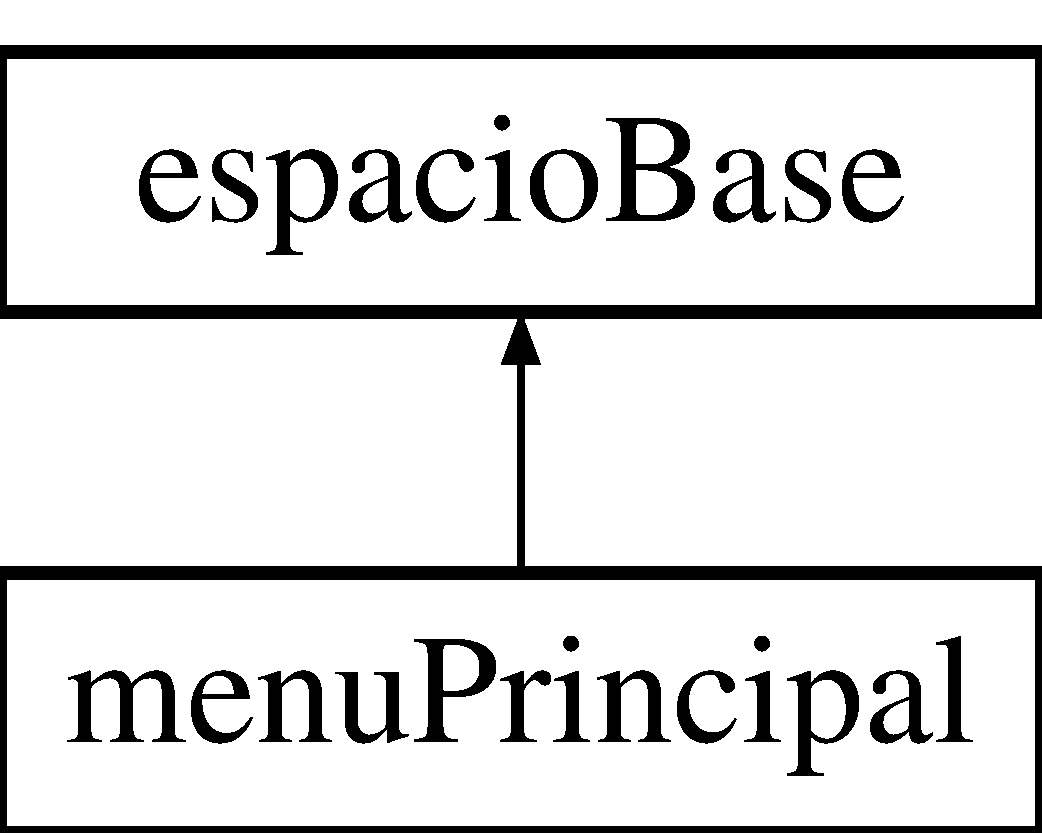
\includegraphics[height=2.000000cm]{classmenu_principal}
\end{center}
\end{figure}
\subsection*{Métodos públicos}
\begin{DoxyCompactItemize}
\item 
\hyperlink{classmenu_principal_a28bc45a9592e32d48979bb34b5e937b5}{menu\+Principal} ()
\begin{DoxyCompactList}\small\item\em Constructor de la clase. \end{DoxyCompactList}\item 
\hyperlink{classmenu_principal_aec2f0d44f0cd26e5c9ddfea5141ba0a1}{$\sim$menu\+Principal} ()
\begin{DoxyCompactList}\small\item\em Destructor de la clase. \end{DoxyCompactList}\item 
void \hyperlink{classmenu_principal_af392d4bbd2d1851b565441ed9dccbae8}{setup} ()
\begin{DoxyCompactList}\small\item\em Método inicial del ciclo de Open\+G\+L. \end{DoxyCompactList}\item 
\hyperlink{classespacio_base}{espacio\+Base} $\ast$ \hyperlink{classmenu_principal_a92b6834ff602085f79bb16f39c6a45cd}{update} (float, float)
\begin{DoxyCompactList}\small\item\em Controla tareas lógica de cada ciclo de Open\+G\+L, version tobii. \end{DoxyCompactList}\item 
\hyperlink{classespacio_base}{espacio\+Base} $\ast$ \hyperlink{classmenu_principal_a74169588b3f34d0eec40f0d749a7f03f}{update} (float, float, bool)
\begin{DoxyCompactList}\small\item\em Controla tareas lógica de cada ciclo de Open\+G\+L, version leap. \end{DoxyCompactList}\item 
void \hyperlink{classmenu_principal_ac76c28146574b4b72364cb877b5cd83f}{draw} ()
\begin{DoxyCompactList}\small\item\em Controla las tareas gráficas de cada ciclo de Open\+G\+L. \end{DoxyCompactList}\end{DoxyCompactItemize}
\subsection*{Atributos públicos}
\begin{DoxyCompactItemize}
\item 
\hyperlink{classboton_toggle}{boton\+Toggle} $\ast$ \hyperlink{classmenu_principal_aea487ca8d9e0d1df2fda6a563ca0f04c}{btn\+Input}
\begin{DoxyCompactList}\small\item\em Botón paa cambiar el modo de reconocimiento. \end{DoxyCompactList}\end{DoxyCompactItemize}
\subsection*{Métodos privados}
\begin{DoxyCompactItemize}
\item 
\hyperlink{classespacio_base}{espacio\+Base} $\ast$ \hyperlink{classmenu_principal_a9855069f896926a6e6abace2f30e804e}{update} (bool, bool, bool, bool, bool, bool)
\end{DoxyCompactItemize}
\subsection*{Atributos privados}
\begin{DoxyCompactItemize}
\item 
\hyperlink{classmenu_comunicacion}{menu\+Comunicacion} $\ast$ \hyperlink{classmenu_principal_af820d04d0e35fa1f4c552af95d5e3036}{m\+Comunicacion}
\begin{DoxyCompactList}\small\item\em Instancia del menú de comunicación. \end{DoxyCompactList}\item 
\hyperlink{classmenu_cotidiana}{menu\+Cotidiana} $\ast$ \hyperlink{classmenu_principal_a67ce856e4bf6566b0e2dc4f6c1471e19}{m\+Cotidiana}
\begin{DoxyCompactList}\small\item\em Instancia del menú de vida cotidiana. \end{DoxyCompactList}\item 
\hyperlink{classmenu_ocio}{menu\+Ocio} $\ast$ \hyperlink{classmenu_principal_a8e372431b14d13de965f84dc0593e08a}{m\+Ocio}
\begin{DoxyCompactList}\small\item\em Instancia del menú de ocio. \end{DoxyCompactList}\item 
\hyperlink{classmenu_educacion}{menu\+Educacion} $\ast$ \hyperlink{classmenu_principal_a495c578e5fba7f2453f963e88c193b5d}{m\+Educacion}
\begin{DoxyCompactList}\small\item\em Instancia del menú de educación. \end{DoxyCompactList}\item 
of\+True\+Type\+Font \hyperlink{classmenu_principal_a23f1de2b0d66522eae4ce63763d31ce6}{fuente}
\begin{DoxyCompactList}\small\item\em Fuente del texto. \end{DoxyCompactList}\item 
of\+Image \hyperlink{classmenu_principal_aa5ec7fdf5031285aab08c58e0fecbd82}{logo}
\begin{DoxyCompactList}\small\item\em Logo de la aplicación. \end{DoxyCompactList}\item 
float \hyperlink{classmenu_principal_aca0ebae92aafb9026c9aace3e23463fb}{logox}
\begin{DoxyCompactList}\small\item\em Coordenada x del logo. \end{DoxyCompactList}\item 
float \hyperlink{classmenu_principal_a1f1f6764a1253e7fa12f9cee448f29b9}{logoy}
\begin{DoxyCompactList}\small\item\em Coordenada y del logo. \end{DoxyCompactList}\item 
\hyperlink{classboton_imagen}{boton\+Imagen} $\ast$ \hyperlink{classmenu_principal_a731ca834c77af1bade609b3bc28ab02c}{btn\+Comunicacion}
\begin{DoxyCompactList}\small\item\em Botón de la categoría comunicación. \end{DoxyCompactList}\item 
\hyperlink{classboton_imagen}{boton\+Imagen} $\ast$ \hyperlink{classmenu_principal_ab26a999803f322e9c9f05acd53125a8c}{btn\+Educacion}
\begin{DoxyCompactList}\small\item\em Botón de la categoría educación. \end{DoxyCompactList}\item 
\hyperlink{classboton_imagen}{boton\+Imagen} $\ast$ \hyperlink{classmenu_principal_a9c27d54b3333900acd941d889019ba1a}{btn\+Cotidiana}
\begin{DoxyCompactList}\small\item\em Botón de la categoría vida cotidiana. \end{DoxyCompactList}\item 
\hyperlink{classboton_imagen}{boton\+Imagen} $\ast$ \hyperlink{classmenu_principal_a488846721d51f37a0ce23bb19372c0b1}{btn\+Ocio}
\begin{DoxyCompactList}\small\item\em Botón de la categoría ocio. \end{DoxyCompactList}\item 
\hyperlink{classboton_imagen}{boton\+Imagen} $\ast$ \hyperlink{classmenu_principal_a9415d04ae2ac0a7927c32c95acdcb9ca}{btn\+Salir}
\begin{DoxyCompactList}\small\item\em Botón para salir de la aplicación. \end{DoxyCompactList}\end{DoxyCompactItemize}
\subsection*{Otros miembros heredados}


\subsection{Descripción detallada}
Menú principal de la aplicación. 

Este menú no tiene archivo de configuración sino que los botones están definidos manualmente. Cualquier submenú nuevo deber ser agregado acá. 

\subsection{Documentación del constructor y destructor}
\hypertarget{classmenu_principal_a28bc45a9592e32d48979bb34b5e937b5}{}\index{menu\+Principal@{menu\+Principal}!menu\+Principal@{menu\+Principal}}
\index{menu\+Principal@{menu\+Principal}!menu\+Principal@{menu\+Principal}}
\subsubsection[{menu\+Principal()}]{\setlength{\rightskip}{0pt plus 5cm}menu\+Principal\+::menu\+Principal (
\begin{DoxyParamCaption}
{}
\end{DoxyParamCaption}
)}\label{classmenu_principal_a28bc45a9592e32d48979bb34b5e937b5}


Constructor de la clase. 

Define el modo en que el usuario va a interactuar, ya sea por visión o por gestos. \hypertarget{classmenu_principal_aec2f0d44f0cd26e5c9ddfea5141ba0a1}{}\index{menu\+Principal@{menu\+Principal}!````~menu\+Principal@{$\sim$menu\+Principal}}
\index{````~menu\+Principal@{$\sim$menu\+Principal}!menu\+Principal@{menu\+Principal}}
\subsubsection[{$\sim$menu\+Principal()}]{\setlength{\rightskip}{0pt plus 5cm}menu\+Principal\+::$\sim$menu\+Principal (
\begin{DoxyParamCaption}
{}
\end{DoxyParamCaption}
)}\label{classmenu_principal_aec2f0d44f0cd26e5c9ddfea5141ba0a1}


Destructor de la clase. 



\subsection{Documentación de las funciones miembro}
\hypertarget{classmenu_principal_ac76c28146574b4b72364cb877b5cd83f}{}\index{menu\+Principal@{menu\+Principal}!draw@{draw}}
\index{draw@{draw}!menu\+Principal@{menu\+Principal}}
\subsubsection[{draw()}]{\setlength{\rightskip}{0pt plus 5cm}void menu\+Principal\+::draw (
\begin{DoxyParamCaption}
{}
\end{DoxyParamCaption}
)\hspace{0.3cm}{\ttfamily [virtual]}}\label{classmenu_principal_ac76c28146574b4b72364cb877b5cd83f}


Controla las tareas gráficas de cada ciclo de Open\+G\+L. 



Implementa \hyperlink{classespacio_base_a01b3e668211b6159784f79a3f5a32d95}{espacio\+Base}.

\hypertarget{classmenu_principal_af392d4bbd2d1851b565441ed9dccbae8}{}\index{menu\+Principal@{menu\+Principal}!setup@{setup}}
\index{setup@{setup}!menu\+Principal@{menu\+Principal}}
\subsubsection[{setup()}]{\setlength{\rightskip}{0pt plus 5cm}void menu\+Principal\+::setup (
\begin{DoxyParamCaption}
{}
\end{DoxyParamCaption}
)\hspace{0.3cm}{\ttfamily [virtual]}}\label{classmenu_principal_af392d4bbd2d1851b565441ed9dccbae8}


Método inicial del ciclo de Open\+G\+L. 



Implementa \hyperlink{classespacio_base_a65020ad1e767a235b0c227a1769c5416}{espacio\+Base}.

\hypertarget{classmenu_principal_a92b6834ff602085f79bb16f39c6a45cd}{}\index{menu\+Principal@{menu\+Principal}!update@{update}}
\index{update@{update}!menu\+Principal@{menu\+Principal}}
\subsubsection[{update(float, float)}]{\setlength{\rightskip}{0pt plus 5cm}{\bf espacio\+Base} $\ast$ menu\+Principal\+::update (
\begin{DoxyParamCaption}
\item[{float}]{, }
\item[{float}]{}
\end{DoxyParamCaption}
)\hspace{0.3cm}{\ttfamily [virtual]}}\label{classmenu_principal_a92b6834ff602085f79bb16f39c6a45cd}


Controla tareas lógica de cada ciclo de Open\+G\+L, version tobii. 



Implementa \hyperlink{classespacio_base_abb71ddaa70032182ae4d8370dd05c536}{espacio\+Base}.

\hypertarget{classmenu_principal_a74169588b3f34d0eec40f0d749a7f03f}{}\index{menu\+Principal@{menu\+Principal}!update@{update}}
\index{update@{update}!menu\+Principal@{menu\+Principal}}
\subsubsection[{update(float, float, bool)}]{\setlength{\rightskip}{0pt plus 5cm}{\bf espacio\+Base} $\ast$ menu\+Principal\+::update (
\begin{DoxyParamCaption}
\item[{float}]{, }
\item[{float}]{, }
\item[{bool}]{}
\end{DoxyParamCaption}
)\hspace{0.3cm}{\ttfamily [virtual]}}\label{classmenu_principal_a74169588b3f34d0eec40f0d749a7f03f}


Controla tareas lógica de cada ciclo de Open\+G\+L, version leap. 



Implementa \hyperlink{classespacio_base_afe08700ffb54b8b8191cdea5ec1671ef}{espacio\+Base}.

\hypertarget{classmenu_principal_a9855069f896926a6e6abace2f30e804e}{}\index{menu\+Principal@{menu\+Principal}!update@{update}}
\index{update@{update}!menu\+Principal@{menu\+Principal}}
\subsubsection[{update(bool, bool, bool, bool, bool, bool)}]{\setlength{\rightskip}{0pt plus 5cm}{\bf espacio\+Base} $\ast$ menu\+Principal\+::update (
\begin{DoxyParamCaption}
\item[{bool}]{btn\+Comunicacion\+Res, }
\item[{bool}]{btn\+Educacion\+Res, }
\item[{bool}]{btn\+Cotidiana\+Res, }
\item[{bool}]{btn\+Ocio\+Res, }
\item[{bool}]{btn\+Salir\+Res, }
\item[{bool}]{btn\+Input\+Res}
\end{DoxyParamCaption}
)\hspace{0.3cm}{\ttfamily [private]}}\label{classmenu_principal_a9855069f896926a6e6abace2f30e804e}


\subsection{Documentación de los datos miembro}
\hypertarget{classmenu_principal_a731ca834c77af1bade609b3bc28ab02c}{}\index{menu\+Principal@{menu\+Principal}!btn\+Comunicacion@{btn\+Comunicacion}}
\index{btn\+Comunicacion@{btn\+Comunicacion}!menu\+Principal@{menu\+Principal}}
\subsubsection[{btn\+Comunicacion}]{\setlength{\rightskip}{0pt plus 5cm}{\bf boton\+Imagen}$\ast$ menu\+Principal\+::btn\+Comunicacion\hspace{0.3cm}{\ttfamily [private]}}\label{classmenu_principal_a731ca834c77af1bade609b3bc28ab02c}


Botón de la categoría comunicación. 

\hypertarget{classmenu_principal_a9c27d54b3333900acd941d889019ba1a}{}\index{menu\+Principal@{menu\+Principal}!btn\+Cotidiana@{btn\+Cotidiana}}
\index{btn\+Cotidiana@{btn\+Cotidiana}!menu\+Principal@{menu\+Principal}}
\subsubsection[{btn\+Cotidiana}]{\setlength{\rightskip}{0pt plus 5cm}{\bf boton\+Imagen}$\ast$ menu\+Principal\+::btn\+Cotidiana\hspace{0.3cm}{\ttfamily [private]}}\label{classmenu_principal_a9c27d54b3333900acd941d889019ba1a}


Botón de la categoría vida cotidiana. 

\hypertarget{classmenu_principal_ab26a999803f322e9c9f05acd53125a8c}{}\index{menu\+Principal@{menu\+Principal}!btn\+Educacion@{btn\+Educacion}}
\index{btn\+Educacion@{btn\+Educacion}!menu\+Principal@{menu\+Principal}}
\subsubsection[{btn\+Educacion}]{\setlength{\rightskip}{0pt plus 5cm}{\bf boton\+Imagen}$\ast$ menu\+Principal\+::btn\+Educacion\hspace{0.3cm}{\ttfamily [private]}}\label{classmenu_principal_ab26a999803f322e9c9f05acd53125a8c}


Botón de la categoría educación. 

\hypertarget{classmenu_principal_aea487ca8d9e0d1df2fda6a563ca0f04c}{}\index{menu\+Principal@{menu\+Principal}!btn\+Input@{btn\+Input}}
\index{btn\+Input@{btn\+Input}!menu\+Principal@{menu\+Principal}}
\subsubsection[{btn\+Input}]{\setlength{\rightskip}{0pt plus 5cm}{\bf boton\+Toggle}$\ast$ menu\+Principal\+::btn\+Input}\label{classmenu_principal_aea487ca8d9e0d1df2fda6a563ca0f04c}


Botón paa cambiar el modo de reconocimiento. 

\hypertarget{classmenu_principal_a488846721d51f37a0ce23bb19372c0b1}{}\index{menu\+Principal@{menu\+Principal}!btn\+Ocio@{btn\+Ocio}}
\index{btn\+Ocio@{btn\+Ocio}!menu\+Principal@{menu\+Principal}}
\subsubsection[{btn\+Ocio}]{\setlength{\rightskip}{0pt plus 5cm}{\bf boton\+Imagen}$\ast$ menu\+Principal\+::btn\+Ocio\hspace{0.3cm}{\ttfamily [private]}}\label{classmenu_principal_a488846721d51f37a0ce23bb19372c0b1}


Botón de la categoría ocio. 

\hypertarget{classmenu_principal_a9415d04ae2ac0a7927c32c95acdcb9ca}{}\index{menu\+Principal@{menu\+Principal}!btn\+Salir@{btn\+Salir}}
\index{btn\+Salir@{btn\+Salir}!menu\+Principal@{menu\+Principal}}
\subsubsection[{btn\+Salir}]{\setlength{\rightskip}{0pt plus 5cm}{\bf boton\+Imagen}$\ast$ menu\+Principal\+::btn\+Salir\hspace{0.3cm}{\ttfamily [private]}}\label{classmenu_principal_a9415d04ae2ac0a7927c32c95acdcb9ca}


Botón para salir de la aplicación. 

\hypertarget{classmenu_principal_a23f1de2b0d66522eae4ce63763d31ce6}{}\index{menu\+Principal@{menu\+Principal}!fuente@{fuente}}
\index{fuente@{fuente}!menu\+Principal@{menu\+Principal}}
\subsubsection[{fuente}]{\setlength{\rightskip}{0pt plus 5cm}of\+True\+Type\+Font menu\+Principal\+::fuente\hspace{0.3cm}{\ttfamily [private]}}\label{classmenu_principal_a23f1de2b0d66522eae4ce63763d31ce6}


Fuente del texto. 

\hypertarget{classmenu_principal_aa5ec7fdf5031285aab08c58e0fecbd82}{}\index{menu\+Principal@{menu\+Principal}!logo@{logo}}
\index{logo@{logo}!menu\+Principal@{menu\+Principal}}
\subsubsection[{logo}]{\setlength{\rightskip}{0pt plus 5cm}of\+Image menu\+Principal\+::logo\hspace{0.3cm}{\ttfamily [private]}}\label{classmenu_principal_aa5ec7fdf5031285aab08c58e0fecbd82}


Logo de la aplicación. 

\hypertarget{classmenu_principal_aca0ebae92aafb9026c9aace3e23463fb}{}\index{menu\+Principal@{menu\+Principal}!logox@{logox}}
\index{logox@{logox}!menu\+Principal@{menu\+Principal}}
\subsubsection[{logox}]{\setlength{\rightskip}{0pt plus 5cm}float menu\+Principal\+::logox\hspace{0.3cm}{\ttfamily [private]}}\label{classmenu_principal_aca0ebae92aafb9026c9aace3e23463fb}


Coordenada x del logo. 

\hypertarget{classmenu_principal_a1f1f6764a1253e7fa12f9cee448f29b9}{}\index{menu\+Principal@{menu\+Principal}!logoy@{logoy}}
\index{logoy@{logoy}!menu\+Principal@{menu\+Principal}}
\subsubsection[{logoy}]{\setlength{\rightskip}{0pt plus 5cm}float menu\+Principal\+::logoy\hspace{0.3cm}{\ttfamily [private]}}\label{classmenu_principal_a1f1f6764a1253e7fa12f9cee448f29b9}


Coordenada y del logo. 

\hypertarget{classmenu_principal_af820d04d0e35fa1f4c552af95d5e3036}{}\index{menu\+Principal@{menu\+Principal}!m\+Comunicacion@{m\+Comunicacion}}
\index{m\+Comunicacion@{m\+Comunicacion}!menu\+Principal@{menu\+Principal}}
\subsubsection[{m\+Comunicacion}]{\setlength{\rightskip}{0pt plus 5cm}{\bf menu\+Comunicacion}$\ast$ menu\+Principal\+::m\+Comunicacion\hspace{0.3cm}{\ttfamily [private]}}\label{classmenu_principal_af820d04d0e35fa1f4c552af95d5e3036}


Instancia del menú de comunicación. 

\hypertarget{classmenu_principal_a67ce856e4bf6566b0e2dc4f6c1471e19}{}\index{menu\+Principal@{menu\+Principal}!m\+Cotidiana@{m\+Cotidiana}}
\index{m\+Cotidiana@{m\+Cotidiana}!menu\+Principal@{menu\+Principal}}
\subsubsection[{m\+Cotidiana}]{\setlength{\rightskip}{0pt plus 5cm}{\bf menu\+Cotidiana}$\ast$ menu\+Principal\+::m\+Cotidiana\hspace{0.3cm}{\ttfamily [private]}}\label{classmenu_principal_a67ce856e4bf6566b0e2dc4f6c1471e19}


Instancia del menú de vida cotidiana. 

\hypertarget{classmenu_principal_a495c578e5fba7f2453f963e88c193b5d}{}\index{menu\+Principal@{menu\+Principal}!m\+Educacion@{m\+Educacion}}
\index{m\+Educacion@{m\+Educacion}!menu\+Principal@{menu\+Principal}}
\subsubsection[{m\+Educacion}]{\setlength{\rightskip}{0pt plus 5cm}{\bf menu\+Educacion}$\ast$ menu\+Principal\+::m\+Educacion\hspace{0.3cm}{\ttfamily [private]}}\label{classmenu_principal_a495c578e5fba7f2453f963e88c193b5d}


Instancia del menú de educación. 

\hypertarget{classmenu_principal_a8e372431b14d13de965f84dc0593e08a}{}\index{menu\+Principal@{menu\+Principal}!m\+Ocio@{m\+Ocio}}
\index{m\+Ocio@{m\+Ocio}!menu\+Principal@{menu\+Principal}}
\subsubsection[{m\+Ocio}]{\setlength{\rightskip}{0pt plus 5cm}{\bf menu\+Ocio}$\ast$ menu\+Principal\+::m\+Ocio\hspace{0.3cm}{\ttfamily [private]}}\label{classmenu_principal_a8e372431b14d13de965f84dc0593e08a}


Instancia del menú de ocio. 



La documentación para esta clase fue generada a partir de los siguientes ficheros\+:\begin{DoxyCompactItemize}
\item 
C\+:/of\+\_\+v0.\+8.\+4\+\_\+vs\+\_\+release/apps/my\+Apps/\+Robo\+Tracking\+App/src/menus/\hyperlink{menu_principal_8h}{menu\+Principal.\+h}\item 
C\+:/of\+\_\+v0.\+8.\+4\+\_\+vs\+\_\+release/apps/my\+Apps/\+Robo\+Tracking\+App/src/menus/\hyperlink{menu_principal_8cpp}{menu\+Principal.\+cpp}\end{DoxyCompactItemize}

\hypertarget{classof_app}{}\section{Referencia de la Clase of\+App}
\label{classof_app}\index{of\+App@{of\+App}}


Clase base que coordina la interacción entre el ciclo de Open\+G\+L y la aplicación como tal.  




{\ttfamily \#include $<$of\+App.\+h$>$}

Diagrama de herencias de of\+App\begin{figure}[H]
\begin{center}
\leavevmode
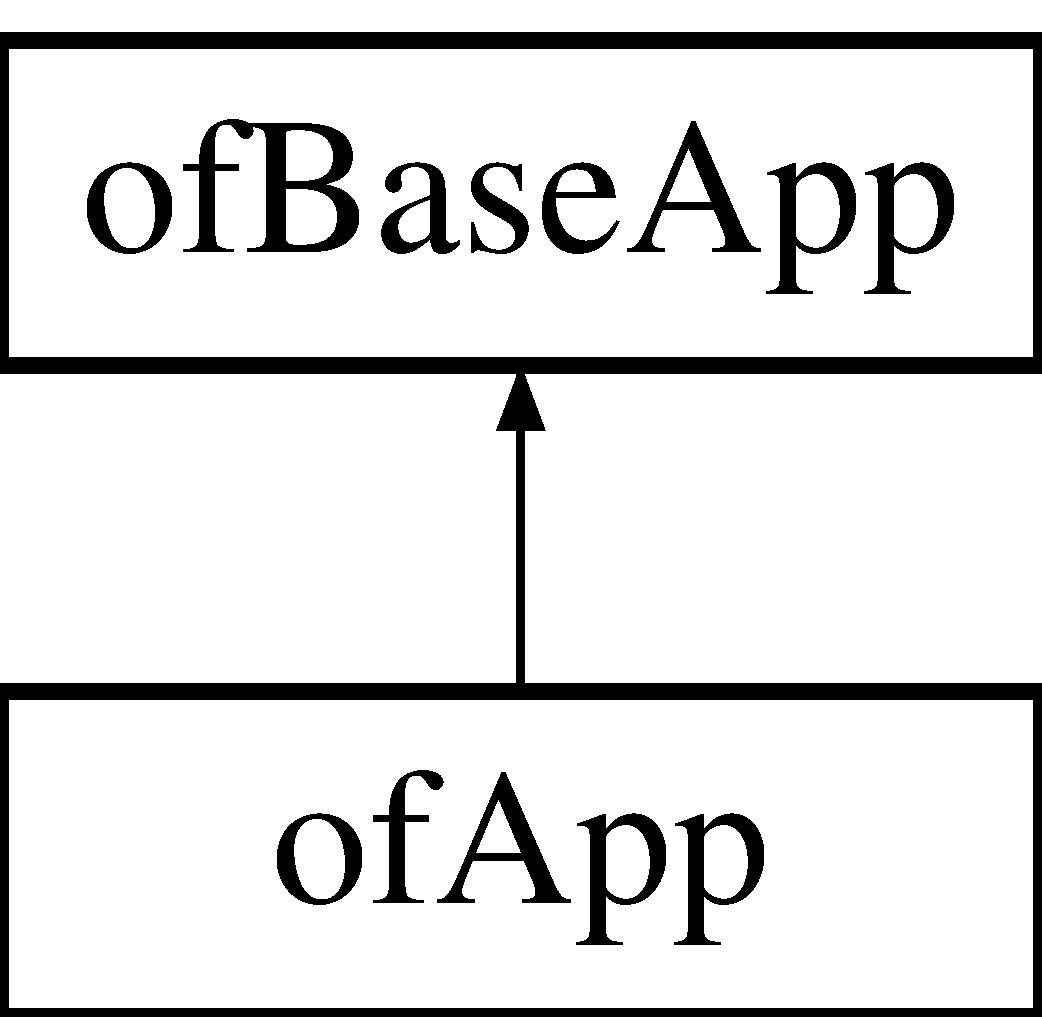
\includegraphics[height=2.000000cm]{classof_app}
\end{center}
\end{figure}
\subsection*{Métodos públicos}
\begin{DoxyCompactItemize}
\item 
\hyperlink{classof_app_a8e51b68c569cf4839163fd7470d50260}{of\+App} (int, int)
\begin{DoxyCompactList}\small\item\em Constructor de la clase. \end{DoxyCompactList}\item 
\hyperlink{classof_app_a46d5e370034c47f5fc1a530bcb331c27}{$\sim$of\+App} ()
\begin{DoxyCompactList}\small\item\em Destructor de la clase. \end{DoxyCompactList}\item 
void \hyperlink{classof_app_af68eaa1366244f7a541cd08e02199c12}{setup} ()
\begin{DoxyCompactList}\small\item\em Método inicial del ciclo de Open\+G\+L. \end{DoxyCompactList}\item 
void \hyperlink{classof_app_afef41ea4aee5a22ea530afba33ae7a7b}{update} ()
\begin{DoxyCompactList}\small\item\em Controla tareas lógica de cada ciclo de Open\+G\+L. \end{DoxyCompactList}\item 
void \hyperlink{classof_app_a75dd45437b9e317db73d8daef1ad49f8}{draw} ()
\begin{DoxyCompactList}\small\item\em Controla las tareas gráficas de cada ciclo de Open\+G\+L. \end{DoxyCompactList}\item 
void \hyperlink{classof_app_a957d3197364bbac8e67eaa4f15b28ad3}{key\+Pressed} (int key)
\begin{DoxyCompactList}\small\item\em Se activa cada vez que el usuario presiona una tecla. \end{DoxyCompactList}\item 
void \hyperlink{classof_app_aa1503a87453bcfdd395fe4acca5d91a0}{key\+Released} (int key)
\begin{DoxyCompactList}\small\item\em Se activa cada vez que el usuario suelta una tecla. \end{DoxyCompactList}\item 
void \hyperlink{classof_app_a158b41a606310db4633fdb817b21047c}{mouse\+Moved} (int x, int y)
\begin{DoxyCompactList}\small\item\em Se activa cuando el mouse se mueve de posición. \end{DoxyCompactList}\item 
void \hyperlink{classof_app_a1ec53d1be799dc275806ff6c6548cd83}{mouse\+Dragged} (int x, int y, int button)
\begin{DoxyCompactList}\small\item\em Se activa cuando el usuario arrastra el mouse dejando cierto botón apretado. \end{DoxyCompactList}\item 
void \hyperlink{classof_app_a2c2ea9c160231e55424dfd98466ef27d}{mouse\+Pressed} (int x, int y, int button)
\begin{DoxyCompactList}\small\item\em Se activa cuando el usuario presiona un botón del mouse. \end{DoxyCompactList}\item 
void \hyperlink{classof_app_aa3131f1554fc49eaa9ee0f284e48129b}{mouse\+Released} (int x, int y, int button)
\begin{DoxyCompactList}\small\item\em Se activa cuando el usuario suelta un botón del mouse. \end{DoxyCompactList}\item 
void \hyperlink{classof_app_ae4dc1ec1513dcbe48bc78a5e4c3fac0f}{window\+Resized} (int w, int h)
\begin{DoxyCompactList}\small\item\em Se activa cuando la ventana cambia de tamaño. \end{DoxyCompactList}\item 
void \hyperlink{classof_app_aada5a79556321801567752a0e5a69bda}{drag\+Event} (of\+Drag\+Info drag\+Info)
\item 
void \hyperlink{classof_app_a885672a72340a5e998af1d16718dc766}{got\+Message} (of\+Message msg)
\end{DoxyCompactItemize}
\subsection*{Atributos públicos}
\begin{DoxyCompactItemize}
\item 
bool \hyperlink{classof_app_ac06e7f62949f8d76a68ea3020ff21da3}{input\+Mode}
\begin{DoxyCompactList}\small\item\em Define el modo actual de entrada (visión o gestos) \end{DoxyCompactList}\end{DoxyCompactItemize}
\subsection*{Atributos privados}
\begin{DoxyCompactItemize}
\item 
Controller $\ast$ \hyperlink{classof_app_aaca01b1fe9aa8a406ca09a5c4ede5f99}{controller}
\item 
\hyperlink{classespacio_base}{espacio\+Base} $\ast$ \hyperlink{classof_app_a1e3e4e9da97b2a839dd1255c65f73453}{espacio\+Activo}
\begin{DoxyCompactList}\small\item\em Instancia del espacio activo en la pantalla. \end{DoxyCompactList}\item 
\hyperlink{classmenu_principal}{menu\+Principal} $\ast$ \hyperlink{classof_app_a9ba8bf05bd3a0932461179f47759b83d}{m\+Principal}
\begin{DoxyCompactList}\small\item\em Instancia del menú principal de la aplicación. \end{DoxyCompactList}\item 
int \hyperlink{classof_app_a07b648bd42ef7fda31bf208ccd18d5f8}{tam\+X}
\item 
int \hyperlink{classof_app_ac1e9d00b0014a47490688c3b298a67c9}{tam\+Y}
\item 
int \hyperlink{classof_app_ae5beab7e06a1bedf3a988264d501984c}{leap\+X}
\item 
int \hyperlink{classof_app_a96ce450adbe65fbf40bb099435d7b27d}{leap\+Y}
\item 
bool \hyperlink{classof_app_acd3a56a2f96cc74a240b84649179e79f}{hand\+Pressed}
\item 
Frame \hyperlink{classof_app_a49ee00759b6afa60298b89befa53664f}{last\+Frame}
\end{DoxyCompactItemize}


\subsection{Descripción detallada}
Clase base que coordina la interacción entre el ciclo de Open\+G\+L y la aplicación como tal. 

Esta clase se maneja por medio de los eventos establecidos por Open\+G\+L. Cualquier espacio de la aplicacion debe tener al menos implementado los métodos \hyperlink{classof_app_af68eaa1366244f7a541cd08e02199c12}{setup()}, \hyperlink{classof_app_afef41ea4aee5a22ea530afba33ae7a7b}{update()} y \hyperlink{classof_app_a75dd45437b9e317db73d8daef1ad49f8}{draw()} para que puedan ser inicializados y dibujados en pantalla. Las demás funciones de Open\+G\+L se definen pero se dejan vacías. 

\subsection{Documentación del constructor y destructor}
\hypertarget{classof_app_a8e51b68c569cf4839163fd7470d50260}{}\index{of\+App@{of\+App}!of\+App@{of\+App}}
\index{of\+App@{of\+App}!of\+App@{of\+App}}
\subsubsection[{of\+App(int, int)}]{\setlength{\rightskip}{0pt plus 5cm}of\+App\+::of\+App (
\begin{DoxyParamCaption}
\item[{int}]{x, }
\item[{int}]{y}
\end{DoxyParamCaption}
)}\label{classof_app_a8e51b68c569cf4839163fd7470d50260}


Constructor de la clase. 

Por defecto, inicia la aplicación en modo visión, sin embargo puede definirse un parámetro de constructor para definir el modo desde el main o leerlo desde un archivo de configuración.


\begin{DoxyParams}[1]{Parámetros}
\mbox{\tt in}  & {\em x} & tamaño del largo de la ventana de la aplicación \\
\hline
\mbox{\tt in}  & {\em y} & tamaño del ancho de la ventana de la apliación \\
\hline
\end{DoxyParams}
\hypertarget{classof_app_a46d5e370034c47f5fc1a530bcb331c27}{}\index{of\+App@{of\+App}!````~of\+App@{$\sim$of\+App}}
\index{````~of\+App@{$\sim$of\+App}!of\+App@{of\+App}}
\subsubsection[{$\sim$of\+App()}]{\setlength{\rightskip}{0pt plus 5cm}of\+App\+::$\sim$of\+App (
\begin{DoxyParamCaption}
{}
\end{DoxyParamCaption}
)}\label{classof_app_a46d5e370034c47f5fc1a530bcb331c27}


Destructor de la clase. 

Borra a m\+Principal 

\subsection{Documentación de las funciones miembro}
\hypertarget{classof_app_aada5a79556321801567752a0e5a69bda}{}\index{of\+App@{of\+App}!drag\+Event@{drag\+Event}}
\index{drag\+Event@{drag\+Event}!of\+App@{of\+App}}
\subsubsection[{drag\+Event(of\+Drag\+Info drag\+Info)}]{\setlength{\rightskip}{0pt plus 5cm}void of\+App\+::drag\+Event (
\begin{DoxyParamCaption}
\item[{of\+Drag\+Info}]{drag\+Info}
\end{DoxyParamCaption}
)}\label{classof_app_aada5a79556321801567752a0e5a69bda}
\hypertarget{classof_app_a75dd45437b9e317db73d8daef1ad49f8}{}\index{of\+App@{of\+App}!draw@{draw}}
\index{draw@{draw}!of\+App@{of\+App}}
\subsubsection[{draw()}]{\setlength{\rightskip}{0pt plus 5cm}void of\+App\+::draw (
\begin{DoxyParamCaption}
{}
\end{DoxyParamCaption}
)}\label{classof_app_a75dd45437b9e317db73d8daef1ad49f8}


Controla las tareas gráficas de cada ciclo de Open\+G\+L. 

Aquí se realizan todas la tareas de dibujar elementos en pantalla. Este método dibuja la representación de la entrada (ya sea por pupilas o por gestos). Además se encarga de llamar al \hyperlink{classof_app_a75dd45437b9e317db73d8daef1ad49f8}{draw()} del espacio activo.

La forma en la que se dibuja en la pantalla es por orden de llamados. Las cosas que se llamen a dibujar de primero van a quedar \char`\"{}al fondo\char`\"{}. \hypertarget{classof_app_a885672a72340a5e998af1d16718dc766}{}\index{of\+App@{of\+App}!got\+Message@{got\+Message}}
\index{got\+Message@{got\+Message}!of\+App@{of\+App}}
\subsubsection[{got\+Message(of\+Message msg)}]{\setlength{\rightskip}{0pt plus 5cm}void of\+App\+::got\+Message (
\begin{DoxyParamCaption}
\item[{of\+Message}]{msg}
\end{DoxyParamCaption}
)}\label{classof_app_a885672a72340a5e998af1d16718dc766}
\hypertarget{classof_app_a957d3197364bbac8e67eaa4f15b28ad3}{}\index{of\+App@{of\+App}!key\+Pressed@{key\+Pressed}}
\index{key\+Pressed@{key\+Pressed}!of\+App@{of\+App}}
\subsubsection[{key\+Pressed(int key)}]{\setlength{\rightskip}{0pt plus 5cm}void of\+App\+::key\+Pressed (
\begin{DoxyParamCaption}
\item[{int}]{key}
\end{DoxyParamCaption}
)}\label{classof_app_a957d3197364bbac8e67eaa4f15b28ad3}


Se activa cada vez que el usuario presiona una tecla. 

\hypertarget{classof_app_aa1503a87453bcfdd395fe4acca5d91a0}{}\index{of\+App@{of\+App}!key\+Released@{key\+Released}}
\index{key\+Released@{key\+Released}!of\+App@{of\+App}}
\subsubsection[{key\+Released(int key)}]{\setlength{\rightskip}{0pt plus 5cm}void of\+App\+::key\+Released (
\begin{DoxyParamCaption}
\item[{int}]{key}
\end{DoxyParamCaption}
)}\label{classof_app_aa1503a87453bcfdd395fe4acca5d91a0}


Se activa cada vez que el usuario suelta una tecla. 

\hypertarget{classof_app_a1ec53d1be799dc275806ff6c6548cd83}{}\index{of\+App@{of\+App}!mouse\+Dragged@{mouse\+Dragged}}
\index{mouse\+Dragged@{mouse\+Dragged}!of\+App@{of\+App}}
\subsubsection[{mouse\+Dragged(int x, int y, int button)}]{\setlength{\rightskip}{0pt plus 5cm}void of\+App\+::mouse\+Dragged (
\begin{DoxyParamCaption}
\item[{int}]{x, }
\item[{int}]{y, }
\item[{int}]{button}
\end{DoxyParamCaption}
)}\label{classof_app_a1ec53d1be799dc275806ff6c6548cd83}


Se activa cuando el usuario arrastra el mouse dejando cierto botón apretado. 

\hypertarget{classof_app_a158b41a606310db4633fdb817b21047c}{}\index{of\+App@{of\+App}!mouse\+Moved@{mouse\+Moved}}
\index{mouse\+Moved@{mouse\+Moved}!of\+App@{of\+App}}
\subsubsection[{mouse\+Moved(int x, int y)}]{\setlength{\rightskip}{0pt plus 5cm}void of\+App\+::mouse\+Moved (
\begin{DoxyParamCaption}
\item[{int}]{x, }
\item[{int}]{y}
\end{DoxyParamCaption}
)}\label{classof_app_a158b41a606310db4633fdb817b21047c}


Se activa cuando el mouse se mueve de posición. 

\hypertarget{classof_app_a2c2ea9c160231e55424dfd98466ef27d}{}\index{of\+App@{of\+App}!mouse\+Pressed@{mouse\+Pressed}}
\index{mouse\+Pressed@{mouse\+Pressed}!of\+App@{of\+App}}
\subsubsection[{mouse\+Pressed(int x, int y, int button)}]{\setlength{\rightskip}{0pt plus 5cm}void of\+App\+::mouse\+Pressed (
\begin{DoxyParamCaption}
\item[{int}]{x, }
\item[{int}]{y, }
\item[{int}]{button}
\end{DoxyParamCaption}
)}\label{classof_app_a2c2ea9c160231e55424dfd98466ef27d}


Se activa cuando el usuario presiona un botón del mouse. 

\hypertarget{classof_app_aa3131f1554fc49eaa9ee0f284e48129b}{}\index{of\+App@{of\+App}!mouse\+Released@{mouse\+Released}}
\index{mouse\+Released@{mouse\+Released}!of\+App@{of\+App}}
\subsubsection[{mouse\+Released(int x, int y, int button)}]{\setlength{\rightskip}{0pt plus 5cm}void of\+App\+::mouse\+Released (
\begin{DoxyParamCaption}
\item[{int}]{x, }
\item[{int}]{y, }
\item[{int}]{button}
\end{DoxyParamCaption}
)}\label{classof_app_aa3131f1554fc49eaa9ee0f284e48129b}


Se activa cuando el usuario suelta un botón del mouse. 

\hypertarget{classof_app_af68eaa1366244f7a541cd08e02199c12}{}\index{of\+App@{of\+App}!setup@{setup}}
\index{setup@{setup}!of\+App@{of\+App}}
\subsubsection[{setup()}]{\setlength{\rightskip}{0pt plus 5cm}void of\+App\+::setup (
\begin{DoxyParamCaption}
{}
\end{DoxyParamCaption}
)}\label{classof_app_af68eaa1366244f7a541cd08e02199c12}


Método inicial del ciclo de Open\+G\+L. 

Se pretende que se inicialize todo lo necesario para empezar a dibujar los componentes necesarios de la aplicación.

No se deben confundir tareas de constructor puesto que acá solo se inicializa lo referente a tareas gráficas. \hypertarget{classof_app_afef41ea4aee5a22ea530afba33ae7a7b}{}\index{of\+App@{of\+App}!update@{update}}
\index{update@{update}!of\+App@{of\+App}}
\subsubsection[{update()}]{\setlength{\rightskip}{0pt plus 5cm}void of\+App\+::update (
\begin{DoxyParamCaption}
{}
\end{DoxyParamCaption}
)}\label{classof_app_afef41ea4aee5a22ea530afba33ae7a7b}


Controla tareas lógica de cada ciclo de Open\+G\+L. 

En cada ciclo de Open\+G\+L este método se llama antes de \hyperlink{classof_app_a75dd45437b9e317db73d8daef1ad49f8}{draw()} para actualizar las tareas lógicas de la interfaz gráfica.

Se puede ver esta instancia como un método padre porque invoca al update del espacio que está activo al momento de ejecución. \hypertarget{classof_app_ae4dc1ec1513dcbe48bc78a5e4c3fac0f}{}\index{of\+App@{of\+App}!window\+Resized@{window\+Resized}}
\index{window\+Resized@{window\+Resized}!of\+App@{of\+App}}
\subsubsection[{window\+Resized(int w, int h)}]{\setlength{\rightskip}{0pt plus 5cm}void of\+App\+::window\+Resized (
\begin{DoxyParamCaption}
\item[{int}]{w, }
\item[{int}]{h}
\end{DoxyParamCaption}
)}\label{classof_app_ae4dc1ec1513dcbe48bc78a5e4c3fac0f}


Se activa cuando la ventana cambia de tamaño. 



\subsection{Documentación de los datos miembro}
\hypertarget{classof_app_aaca01b1fe9aa8a406ca09a5c4ede5f99}{}\index{of\+App@{of\+App}!controller@{controller}}
\index{controller@{controller}!of\+App@{of\+App}}
\subsubsection[{controller}]{\setlength{\rightskip}{0pt plus 5cm}Controller$\ast$ of\+App\+::controller\hspace{0.3cm}{\ttfamily [private]}}\label{classof_app_aaca01b1fe9aa8a406ca09a5c4ede5f99}
\hypertarget{classof_app_a1e3e4e9da97b2a839dd1255c65f73453}{}\index{of\+App@{of\+App}!espacio\+Activo@{espacio\+Activo}}
\index{espacio\+Activo@{espacio\+Activo}!of\+App@{of\+App}}
\subsubsection[{espacio\+Activo}]{\setlength{\rightskip}{0pt plus 5cm}{\bf espacio\+Base}$\ast$ of\+App\+::espacio\+Activo\hspace{0.3cm}{\ttfamily [private]}}\label{classof_app_a1e3e4e9da97b2a839dd1255c65f73453}


Instancia del espacio activo en la pantalla. 

Este puntero se mueve dinámicamente. Si un espacio necesita cambiar a otro solo necesita modificar el puntero hacia el espacio que se quiere activar y el ciclo de Open\+G\+L se encarga de invocar a sus debidos métodos.

Si el puntero llega alguna vez a ser 0 representa la salida del programa. \hypertarget{classof_app_acd3a56a2f96cc74a240b84649179e79f}{}\index{of\+App@{of\+App}!hand\+Pressed@{hand\+Pressed}}
\index{hand\+Pressed@{hand\+Pressed}!of\+App@{of\+App}}
\subsubsection[{hand\+Pressed}]{\setlength{\rightskip}{0pt plus 5cm}bool of\+App\+::hand\+Pressed\hspace{0.3cm}{\ttfamily [private]}}\label{classof_app_acd3a56a2f96cc74a240b84649179e79f}
\hypertarget{classof_app_ac06e7f62949f8d76a68ea3020ff21da3}{}\index{of\+App@{of\+App}!input\+Mode@{input\+Mode}}
\index{input\+Mode@{input\+Mode}!of\+App@{of\+App}}
\subsubsection[{input\+Mode}]{\setlength{\rightskip}{0pt plus 5cm}bool of\+App\+::input\+Mode}\label{classof_app_ac06e7f62949f8d76a68ea3020ff21da3}


Define el modo actual de entrada (visión o gestos) 

\hypertarget{classof_app_a49ee00759b6afa60298b89befa53664f}{}\index{of\+App@{of\+App}!last\+Frame@{last\+Frame}}
\index{last\+Frame@{last\+Frame}!of\+App@{of\+App}}
\subsubsection[{last\+Frame}]{\setlength{\rightskip}{0pt plus 5cm}Frame of\+App\+::last\+Frame\hspace{0.3cm}{\ttfamily [private]}}\label{classof_app_a49ee00759b6afa60298b89befa53664f}
\hypertarget{classof_app_ae5beab7e06a1bedf3a988264d501984c}{}\index{of\+App@{of\+App}!leap\+X@{leap\+X}}
\index{leap\+X@{leap\+X}!of\+App@{of\+App}}
\subsubsection[{leap\+X}]{\setlength{\rightskip}{0pt plus 5cm}int of\+App\+::leap\+X\hspace{0.3cm}{\ttfamily [private]}}\label{classof_app_ae5beab7e06a1bedf3a988264d501984c}
\hypertarget{classof_app_a96ce450adbe65fbf40bb099435d7b27d}{}\index{of\+App@{of\+App}!leap\+Y@{leap\+Y}}
\index{leap\+Y@{leap\+Y}!of\+App@{of\+App}}
\subsubsection[{leap\+Y}]{\setlength{\rightskip}{0pt plus 5cm}int of\+App\+::leap\+Y\hspace{0.3cm}{\ttfamily [private]}}\label{classof_app_a96ce450adbe65fbf40bb099435d7b27d}
\hypertarget{classof_app_a9ba8bf05bd3a0932461179f47759b83d}{}\index{of\+App@{of\+App}!m\+Principal@{m\+Principal}}
\index{m\+Principal@{m\+Principal}!of\+App@{of\+App}}
\subsubsection[{m\+Principal}]{\setlength{\rightskip}{0pt plus 5cm}{\bf menu\+Principal}$\ast$ of\+App\+::m\+Principal\hspace{0.3cm}{\ttfamily [private]}}\label{classof_app_a9ba8bf05bd3a0932461179f47759b83d}


Instancia del menú principal de la aplicación. 

\hypertarget{classof_app_a07b648bd42ef7fda31bf208ccd18d5f8}{}\index{of\+App@{of\+App}!tam\+X@{tam\+X}}
\index{tam\+X@{tam\+X}!of\+App@{of\+App}}
\subsubsection[{tam\+X}]{\setlength{\rightskip}{0pt plus 5cm}int of\+App\+::tam\+X\hspace{0.3cm}{\ttfamily [private]}}\label{classof_app_a07b648bd42ef7fda31bf208ccd18d5f8}
\hypertarget{classof_app_ac1e9d00b0014a47490688c3b298a67c9}{}\index{of\+App@{of\+App}!tam\+Y@{tam\+Y}}
\index{tam\+Y@{tam\+Y}!of\+App@{of\+App}}
\subsubsection[{tam\+Y}]{\setlength{\rightskip}{0pt plus 5cm}int of\+App\+::tam\+Y\hspace{0.3cm}{\ttfamily [private]}}\label{classof_app_ac1e9d00b0014a47490688c3b298a67c9}


La documentación para esta clase fue generada a partir de los siguientes ficheros\+:\begin{DoxyCompactItemize}
\item 
C\+:/of\+\_\+v0.\+8.\+4\+\_\+vs\+\_\+release/apps/my\+Apps/\+Robo\+Tracking\+App/src/\hyperlink{of_app_8h}{of\+App.\+h}\item 
C\+:/of\+\_\+v0.\+8.\+4\+\_\+vs\+\_\+release/apps/my\+Apps/\+Robo\+Tracking\+App/src/\hyperlink{of_app_8cpp}{of\+App.\+cpp}\end{DoxyCompactItemize}

\hypertarget{classsqlite3_manager}{}\section{Referencia de la Clase sqlite3\+Manager}
\label{classsqlite3_manager}\index{sqlite3\+Manager@{sqlite3\+Manager}}


Maneja la interacción con la base de datos S\+Q\+Lite.  




{\ttfamily \#include $<$sqlite3\+Manager.\+h$>$}

\subsection*{Métodos públicos}
\begin{DoxyCompactItemize}
\item 
\hyperlink{classsqlite3_manager_ae1ae1bbb453ea690ef68f5ea1a9b39ed}{sqlite3\+Manager} (char $\ast$)
\begin{DoxyCompactList}\small\item\em Constructor de la clase. \end{DoxyCompactList}\item 
\hyperlink{classsqlite3_manager_ad03a31151cbc5ccc52f0c2936bddb34b}{$\sim$sqlite3\+Manager} ()
\begin{DoxyCompactList}\small\item\em Destructor de la clase. \end{DoxyCompactList}\item 
vector$<$ vector$<$ string $>$ $>$ \hyperlink{classsqlite3_manager_ad619df24f9d979b179df8a472340a31e}{execute\+Statement} (char $\ast$)
\begin{DoxyCompactList}\small\item\em Ejecuta una sentencia S\+Q\+L. \end{DoxyCompactList}\item 
void \hyperlink{classsqlite3_manager_ac3b8080a48f4fa15df51d32f66f169eb}{print\+Table} (vector$<$ vector$<$ string $>$$>$)
\begin{DoxyCompactList}\small\item\em Imprime una tabla en consola. \end{DoxyCompactList}\end{DoxyCompactItemize}
\subsection*{Atributos privados}
\begin{DoxyCompactItemize}
\item 
sqlite3 $\ast$ \hyperlink{classsqlite3_manager_a9ccf7ca16db10c327a05a5a90f6ee1a5}{db}
\begin{DoxyCompactList}\small\item\em Instancia de la base de datos. \end{DoxyCompactList}\end{DoxyCompactItemize}


\subsection{Descripción detallada}
Maneja la interacción con la base de datos S\+Q\+Lite. 

S\+Q\+Lite es un sistema que implementa un motor S\+Q\+L para manejar una base de datos local. Esta clase engloba las operaciones necesarias para interactuar con un sistema sqlite3 de forma amigable. No están implementadas todas las funcionalidades que S\+Q\+Lite ofrece, sin embargo se motiva a que esta clase sea extendida y reutilizada.

Para más información visitar \href{https://www.sqlite.org/}{\tt https\+://www.\+sqlite.\+org/} y \href{http://www.tutorialspoint.com/sqlite/sqlite_c_cpp.htm}{\tt http\+://www.\+tutorialspoint.\+com/sqlite/sqlite\+\_\+c\+\_\+cpp.\+htm} para una mejor referencia del A\+P\+I C/\+C++.

Para crear y poblar la base de datos es mucho más cómodo utilizar una herramienta de terceros para armar las tablas e insertar datos en un ambiente al estilo D\+B\+M\+S. Se recomienda el uso de la herramienta S\+Q\+Lite\+Spy 

\subsection{Documentación del constructor y destructor}
\hypertarget{classsqlite3_manager_ae1ae1bbb453ea690ef68f5ea1a9b39ed}{}\index{sqlite3\+Manager@{sqlite3\+Manager}!sqlite3\+Manager@{sqlite3\+Manager}}
\index{sqlite3\+Manager@{sqlite3\+Manager}!sqlite3\+Manager@{sqlite3\+Manager}}
\subsubsection[{sqlite3\+Manager(char $\ast$)}]{\setlength{\rightskip}{0pt plus 5cm}sqlite3\+Manager\+::sqlite3\+Manager (
\begin{DoxyParamCaption}
\item[{char $\ast$}]{db\+Location}
\end{DoxyParamCaption}
)}\label{classsqlite3_manager_ae1ae1bbb453ea690ef68f5ea1a9b39ed}


Constructor de la clase. 

Dado un archivo con formado S\+Q\+Lite lo abre para poder ejecutar operaciones sobre la base de datos.


\begin{DoxyParams}{Parámetros}
{\em db\+Location} & Lugar dentro del proyecto donde se encuentra ubicada la base de datos. \\
\hline
\end{DoxyParams}
\hypertarget{classsqlite3_manager_ad03a31151cbc5ccc52f0c2936bddb34b}{}\index{sqlite3\+Manager@{sqlite3\+Manager}!````~sqlite3\+Manager@{$\sim$sqlite3\+Manager}}
\index{````~sqlite3\+Manager@{$\sim$sqlite3\+Manager}!sqlite3\+Manager@{sqlite3\+Manager}}
\subsubsection[{$\sim$sqlite3\+Manager()}]{\setlength{\rightskip}{0pt plus 5cm}sqlite3\+Manager\+::$\sim$sqlite3\+Manager (
\begin{DoxyParamCaption}
{}
\end{DoxyParamCaption}
)}\label{classsqlite3_manager_ad03a31151cbc5ccc52f0c2936bddb34b}


Destructor de la clase. 

Cierra la referencia a la base de datos. 

\subsection{Documentación de las funciones miembro}
\hypertarget{classsqlite3_manager_ad619df24f9d979b179df8a472340a31e}{}\index{sqlite3\+Manager@{sqlite3\+Manager}!execute\+Statement@{execute\+Statement}}
\index{execute\+Statement@{execute\+Statement}!sqlite3\+Manager@{sqlite3\+Manager}}
\subsubsection[{execute\+Statement(char $\ast$)}]{\setlength{\rightskip}{0pt plus 5cm}vector$<$ vector$<$ string $>$ $>$ sqlite3\+Manager\+::execute\+Statement (
\begin{DoxyParamCaption}
\item[{char $\ast$}]{sql}
\end{DoxyParamCaption}
)}\label{classsqlite3_manager_ad619df24f9d979b179df8a472340a31e}


Ejecuta una sentencia S\+Q\+L. 

Dada una instruccion se asegura que pueda ser ejecuta y la realiza. Si hay filas en la respuesta las almacena en una matriz de hileras. Notese que de esta forma todo queda almacenado como hileras.


\begin{DoxyParams}{Parámetros}
{\em sql} & Instrucción para ser ejecutada \\
\hline
\end{DoxyParams}
\begin{DoxyReturn}{Devuelve}
Matriz con n filas y m columnas 
\end{DoxyReturn}
\hypertarget{classsqlite3_manager_ac3b8080a48f4fa15df51d32f66f169eb}{}\index{sqlite3\+Manager@{sqlite3\+Manager}!print\+Table@{print\+Table}}
\index{print\+Table@{print\+Table}!sqlite3\+Manager@{sqlite3\+Manager}}
\subsubsection[{print\+Table(vector$<$ vector$<$ string $>$$>$)}]{\setlength{\rightskip}{0pt plus 5cm}void sqlite3\+Manager\+::print\+Table (
\begin{DoxyParamCaption}
\item[{vector$<$ vector$<$ string $>$$>$}]{table}
\end{DoxyParamCaption}
)}\label{classsqlite3_manager_ac3b8080a48f4fa15df51d32f66f169eb}


Imprime una tabla en consola. 



\subsection{Documentación de los datos miembro}
\hypertarget{classsqlite3_manager_a9ccf7ca16db10c327a05a5a90f6ee1a5}{}\index{sqlite3\+Manager@{sqlite3\+Manager}!db@{db}}
\index{db@{db}!sqlite3\+Manager@{sqlite3\+Manager}}
\subsubsection[{db}]{\setlength{\rightskip}{0pt plus 5cm}sqlite3$\ast$ sqlite3\+Manager\+::db\hspace{0.3cm}{\ttfamily [private]}}\label{classsqlite3_manager_a9ccf7ca16db10c327a05a5a90f6ee1a5}


Instancia de la base de datos. 



La documentación para esta clase fue generada a partir de los siguientes ficheros\+:\begin{DoxyCompactItemize}
\item 
C\+:/of\+\_\+v0.\+8.\+4\+\_\+vs\+\_\+release/apps/my\+Apps/\+Robo\+Tracking\+App/src/utilidades/sqlite3\+Manager/\hyperlink{sqlite3_manager_8h}{sqlite3\+Manager.\+h}\item 
C\+:/of\+\_\+v0.\+8.\+4\+\_\+vs\+\_\+release/apps/my\+Apps/\+Robo\+Tracking\+App/src/utilidades/sqlite3\+Manager/\hyperlink{sqlite3_manager_8cpp}{sqlite3\+Manager.\+cpp}\end{DoxyCompactItemize}

\chapter{Documentación de archivos}
\hypertarget{mainpage_8md}{}\section{Referencia del Archivo pages/mainpage.md}
\label{mainpage_8md}\index{pages/mainpage.\+md@{pages/mainpage.\+md}}

\hypertarget{boton_imagen_8cpp}{}\section{Referencia del Archivo C\+:/of\+\_\+v0.8.4\+\_\+vs\+\_\+release/apps/my\+Apps/\+Robo\+Tracking\+App/src/componentes/boton\+Imagen.cpp}
\label{boton_imagen_8cpp}\index{C\+:/of\+\_\+v0.\+8.\+4\+\_\+vs\+\_\+release/apps/my\+Apps/\+Robo\+Tracking\+App/src/componentes/boton\+Imagen.\+cpp@{C\+:/of\+\_\+v0.\+8.\+4\+\_\+vs\+\_\+release/apps/my\+Apps/\+Robo\+Tracking\+App/src/componentes/boton\+Imagen.\+cpp}}
{\ttfamily \#include \char`\"{}boton\+Imagen.\+h\char`\"{}}\\*

\hypertarget{boton_imagen_8h}{}\section{Referencia del Archivo C\+:/of\+\_\+v0.8.4\+\_\+vs\+\_\+release/apps/my\+Apps/\+Robo\+Tracking\+App/src/componentes/boton\+Imagen.h}
\label{boton_imagen_8h}\index{C\+:/of\+\_\+v0.\+8.\+4\+\_\+vs\+\_\+release/apps/my\+Apps/\+Robo\+Tracking\+App/src/componentes/boton\+Imagen.\+h@{C\+:/of\+\_\+v0.\+8.\+4\+\_\+vs\+\_\+release/apps/my\+Apps/\+Robo\+Tracking\+App/src/componentes/boton\+Imagen.\+h}}
{\ttfamily \#include \char`\"{}componente\+Base.\+h\char`\"{}}\\*
{\ttfamily \#include \char`\"{}of\+True\+Type\+Font.\+h\char`\"{}}\\*
{\ttfamily \#include \char`\"{}of\+Image.\+h\char`\"{}}\\*
\subsection*{Clases}
\begin{DoxyCompactItemize}
\item 
class \hyperlink{classboton_imagen}{boton\+Imagen}
\begin{DoxyCompactList}\small\item\em Botón con imagen y texto. \end{DoxyCompactList}\end{DoxyCompactItemize}

\hypertarget{boton_simple_8cpp}{}\section{Referencia del Archivo C\+:/of\+\_\+v0.8.4\+\_\+vs\+\_\+release/apps/my\+Apps/\+Robo\+Tracking\+App/src/componentes/boton\+Simple.cpp}
\label{boton_simple_8cpp}\index{C\+:/of\+\_\+v0.\+8.\+4\+\_\+vs\+\_\+release/apps/my\+Apps/\+Robo\+Tracking\+App/src/componentes/boton\+Simple.\+cpp@{C\+:/of\+\_\+v0.\+8.\+4\+\_\+vs\+\_\+release/apps/my\+Apps/\+Robo\+Tracking\+App/src/componentes/boton\+Simple.\+cpp}}
{\ttfamily \#include \char`\"{}boton\+Simple.\+h\char`\"{}}\\*
{\ttfamily \#include $<$algorithm$>$}\\*
{\ttfamily \#include $<$string$>$}\\*

\hypertarget{boton_simple_8h}{}\section{Referencia del Archivo C\+:/of\+\_\+v0.8.4\+\_\+vs\+\_\+release/apps/my\+Apps/\+Robo\+Tracking\+App/src/componentes/boton\+Simple.h}
\label{boton_simple_8h}\index{C\+:/of\+\_\+v0.\+8.\+4\+\_\+vs\+\_\+release/apps/my\+Apps/\+Robo\+Tracking\+App/src/componentes/boton\+Simple.\+h@{C\+:/of\+\_\+v0.\+8.\+4\+\_\+vs\+\_\+release/apps/my\+Apps/\+Robo\+Tracking\+App/src/componentes/boton\+Simple.\+h}}
{\ttfamily \#include \char`\"{}componente\+Base.\+h\char`\"{}}\\*
{\ttfamily \#include \char`\"{}of\+True\+Type\+Font.\+h\char`\"{}}\\*
\subsection*{Clases}
\begin{DoxyCompactItemize}
\item 
class \hyperlink{classboton_simple}{boton\+Simple}
\begin{DoxyCompactList}\small\item\em Botón con texto. \end{DoxyCompactList}\end{DoxyCompactItemize}

\hypertarget{boton_toggle_8cpp}{}\section{Referencia del Archivo C\+:/of\+\_\+v0.8.4\+\_\+vs\+\_\+release/apps/my\+Apps/\+Robo\+Tracking\+App/src/componentes/boton\+Toggle.cpp}
\label{boton_toggle_8cpp}\index{C\+:/of\+\_\+v0.\+8.\+4\+\_\+vs\+\_\+release/apps/my\+Apps/\+Robo\+Tracking\+App/src/componentes/boton\+Toggle.\+cpp@{C\+:/of\+\_\+v0.\+8.\+4\+\_\+vs\+\_\+release/apps/my\+Apps/\+Robo\+Tracking\+App/src/componentes/boton\+Toggle.\+cpp}}
{\ttfamily \#include \char`\"{}boton\+Toggle.\+h\char`\"{}}\\*

\hypertarget{boton_toggle_8h}{}\section{Referencia del Archivo C\+:/of\+\_\+v0.8.4\+\_\+vs\+\_\+release/apps/my\+Apps/\+Robo\+Tracking\+App/src/componentes/boton\+Toggle.h}
\label{boton_toggle_8h}\index{C\+:/of\+\_\+v0.\+8.\+4\+\_\+vs\+\_\+release/apps/my\+Apps/\+Robo\+Tracking\+App/src/componentes/boton\+Toggle.\+h@{C\+:/of\+\_\+v0.\+8.\+4\+\_\+vs\+\_\+release/apps/my\+Apps/\+Robo\+Tracking\+App/src/componentes/boton\+Toggle.\+h}}
{\ttfamily \#include \char`\"{}boton\+Imagen.\+h\char`\"{}}\\*
\subsection*{Clases}
\begin{DoxyCompactItemize}
\item 
class \hyperlink{classboton_toggle}{boton\+Toggle}
\begin{DoxyCompactList}\small\item\em Botón que alterna dos imagenes y textos. \end{DoxyCompactList}\end{DoxyCompactItemize}

\hypertarget{caja_texto_8cpp}{}\section{Referencia del Archivo C\+:/of\+\_\+v0.8.4\+\_\+vs\+\_\+release/apps/my\+Apps/\+Robo\+Tracking\+App/src/componentes/caja\+Texto.cpp}
\label{caja_texto_8cpp}\index{C\+:/of\+\_\+v0.\+8.\+4\+\_\+vs\+\_\+release/apps/my\+Apps/\+Robo\+Tracking\+App/src/componentes/caja\+Texto.\+cpp@{C\+:/of\+\_\+v0.\+8.\+4\+\_\+vs\+\_\+release/apps/my\+Apps/\+Robo\+Tracking\+App/src/componentes/caja\+Texto.\+cpp}}
{\ttfamily \#include \char`\"{}caja\+Texto.\+h\char`\"{}}\\*

\hypertarget{caja_texto_8h}{}\section{Referencia del Archivo C\+:/of\+\_\+v0.8.4\+\_\+vs\+\_\+release/apps/my\+Apps/\+Robo\+Tracking\+App/src/componentes/caja\+Texto.h}
\label{caja_texto_8h}\index{C\+:/of\+\_\+v0.\+8.\+4\+\_\+vs\+\_\+release/apps/my\+Apps/\+Robo\+Tracking\+App/src/componentes/caja\+Texto.\+h@{C\+:/of\+\_\+v0.\+8.\+4\+\_\+vs\+\_\+release/apps/my\+Apps/\+Robo\+Tracking\+App/src/componentes/caja\+Texto.\+h}}
{\ttfamily \#include \char`\"{}componente\+Base.\+h\char`\"{}}\\*
{\ttfamily \#include \char`\"{}of\+True\+Type\+Font.\+h\char`\"{}}\\*
{\ttfamily \#include \char`\"{}of\+Color.\+h\char`\"{}}\\*
\subsection*{Clases}
\begin{DoxyCompactItemize}
\item 
class \hyperlink{classcaja_texto}{caja\+Texto}
\begin{DoxyCompactList}\small\item\em Caja para mostrar texto. \end{DoxyCompactList}\end{DoxyCompactItemize}

\hypertarget{componente_base_8cpp}{}\section{Referencia del Archivo C\+:/of\+\_\+v0.8.4\+\_\+vs\+\_\+release/apps/my\+Apps/\+Robo\+Tracking\+App/src/componentes/componente\+Base.cpp}
\label{componente_base_8cpp}\index{C\+:/of\+\_\+v0.\+8.\+4\+\_\+vs\+\_\+release/apps/my\+Apps/\+Robo\+Tracking\+App/src/componentes/componente\+Base.\+cpp@{C\+:/of\+\_\+v0.\+8.\+4\+\_\+vs\+\_\+release/apps/my\+Apps/\+Robo\+Tracking\+App/src/componentes/componente\+Base.\+cpp}}
{\ttfamily \#include \char`\"{}componente\+Base.\+h\char`\"{}}\\*
{\ttfamily \#include $<$stdio.\+h$>$}\\*

\hypertarget{componente_base_8h}{}\section{Referencia del Archivo C\+:/of\+\_\+v0.8.4\+\_\+vs\+\_\+release/apps/my\+Apps/\+Robo\+Tracking\+App/src/componentes/componente\+Base.h}
\label{componente_base_8h}\index{C\+:/of\+\_\+v0.\+8.\+4\+\_\+vs\+\_\+release/apps/my\+Apps/\+Robo\+Tracking\+App/src/componentes/componente\+Base.\+h@{C\+:/of\+\_\+v0.\+8.\+4\+\_\+vs\+\_\+release/apps/my\+Apps/\+Robo\+Tracking\+App/src/componentes/componente\+Base.\+h}}
{\ttfamily \#include $<$time.\+h$>$}\\*
{\ttfamily \#include $<$chrono$>$}\\*
{\ttfamily \#include \char`\"{}of\+Rectangle.\+h\char`\"{}}\\*
{\ttfamily \#include \char`\"{}of\+Graphics.\+h\char`\"{}}\\*
\subsection*{Clases}
\begin{DoxyCompactItemize}
\item 
class \hyperlink{classcomponente_base}{componente\+Base}
\begin{DoxyCompactList}\small\item\em Esquema base de los componentes de los espacios. \end{DoxyCompactList}\end{DoxyCompactItemize}

\hypertarget{fabrica_componentes_8h}{}\section{Referencia del Archivo C\+:/of\+\_\+v0.8.4\+\_\+vs\+\_\+release/apps/my\+Apps/\+Robo\+Tracking\+App/src/componentes/fabrica\+Componentes.h}
\label{fabrica_componentes_8h}\index{C\+:/of\+\_\+v0.\+8.\+4\+\_\+vs\+\_\+release/apps/my\+Apps/\+Robo\+Tracking\+App/src/componentes/fabrica\+Componentes.\+h@{C\+:/of\+\_\+v0.\+8.\+4\+\_\+vs\+\_\+release/apps/my\+Apps/\+Robo\+Tracking\+App/src/componentes/fabrica\+Componentes.\+h}}
{\ttfamily \#include \char`\"{}componente\+Base.\+h\char`\"{}}\\*
{\ttfamily \#include \char`\"{}boton\+Simple.\+h\char`\"{}}\\*
{\ttfamily \#include \char`\"{}caja\+Texto.\+h\char`\"{}}\\*
{\ttfamily \#include \char`\"{}of\+Color.\+h\char`\"{}}\\*
{\ttfamily \#include \char`\"{}ofx\+Xml\+Settings.\+h\char`\"{}}\\*
{\ttfamily \#include $<$stdio.\+h$>$}\\*
{\ttfamily \#include $<$vector$>$}\\*
\subsection*{Clases}
\begin{DoxyCompactItemize}
\item 
class \hyperlink{classfabrica_componentes}{fabrica\+Componentes}
\begin{DoxyCompactList}\small\item\em Utilidad para generar componentes a partir de archivos de configuración. \end{DoxyCompactList}\end{DoxyCompactItemize}

\hypertarget{espacio_base_8cpp}{}\section{Referencia del Archivo C\+:/of\+\_\+v0.8.4\+\_\+vs\+\_\+release/apps/my\+Apps/\+Robo\+Tracking\+App/src/espacios/espacio\+Base.cpp}
\label{espacio_base_8cpp}\index{C\+:/of\+\_\+v0.\+8.\+4\+\_\+vs\+\_\+release/apps/my\+Apps/\+Robo\+Tracking\+App/src/espacios/espacio\+Base.\+cpp@{C\+:/of\+\_\+v0.\+8.\+4\+\_\+vs\+\_\+release/apps/my\+Apps/\+Robo\+Tracking\+App/src/espacios/espacio\+Base.\+cpp}}
{\ttfamily \#include \char`\"{}espacio\+Base.\+h\char`\"{}}\\*

\hypertarget{espacio_base_8h}{}\section{Referencia del Archivo C\+:/of\+\_\+v0.8.4\+\_\+vs\+\_\+release/apps/my\+Apps/\+Robo\+Tracking\+App/src/espacios/espacio\+Base.h}
\label{espacio_base_8h}\index{C\+:/of\+\_\+v0.\+8.\+4\+\_\+vs\+\_\+release/apps/my\+Apps/\+Robo\+Tracking\+App/src/espacios/espacio\+Base.\+h@{C\+:/of\+\_\+v0.\+8.\+4\+\_\+vs\+\_\+release/apps/my\+Apps/\+Robo\+Tracking\+App/src/espacios/espacio\+Base.\+h}}
{\ttfamily \#include $<$string$>$}\\*
{\ttfamily \#include \char`\"{}of\+True\+Type\+Font.\+h\char`\"{}}\\*
{\ttfamily \#include \char`\"{}of\+Graphics.\+h\char`\"{}}\\*
\subsection*{Clases}
\begin{DoxyCompactItemize}
\item 
class \hyperlink{classespacio_base}{espacio\+Base}
\begin{DoxyCompactList}\small\item\em Clase base para todos los espacios de la aplicación. \end{DoxyCompactList}\end{DoxyCompactItemize}

\hypertarget{espacio_camara_8cpp}{}\section{Referencia del Archivo C\+:/of\+\_\+v0.8.4\+\_\+vs\+\_\+release/apps/my\+Apps/\+Robo\+Tracking\+App/src/espacios/espacio\+Camara.cpp}
\label{espacio_camara_8cpp}\index{C\+:/of\+\_\+v0.\+8.\+4\+\_\+vs\+\_\+release/apps/my\+Apps/\+Robo\+Tracking\+App/src/espacios/espacio\+Camara.\+cpp@{C\+:/of\+\_\+v0.\+8.\+4\+\_\+vs\+\_\+release/apps/my\+Apps/\+Robo\+Tracking\+App/src/espacios/espacio\+Camara.\+cpp}}
{\ttfamily \#include \char`\"{}espacio\+Camara.\+h\char`\"{}}\\*

\hypertarget{espacio_camara_8h}{}\section{Referencia del Archivo C\+:/of\+\_\+v0.8.4\+\_\+vs\+\_\+release/apps/my\+Apps/\+Robo\+Tracking\+App/src/espacios/espacio\+Camara.h}
\label{espacio_camara_8h}\index{C\+:/of\+\_\+v0.\+8.\+4\+\_\+vs\+\_\+release/apps/my\+Apps/\+Robo\+Tracking\+App/src/espacios/espacio\+Camara.\+h@{C\+:/of\+\_\+v0.\+8.\+4\+\_\+vs\+\_\+release/apps/my\+Apps/\+Robo\+Tracking\+App/src/espacios/espacio\+Camara.\+h}}
{\ttfamily \#include \char`\"{}espacio\+Base.\+h\char`\"{}}\\*
{\ttfamily \#include \char`\"{}of\+Video\+Grabber.\+h\char`\"{}}\\*
{\ttfamily \#include \char`\"{}boton\+Imagen.\+h\char`\"{}}\\*
\subsection*{Clases}
\begin{DoxyCompactItemize}
\item 
class \hyperlink{classespacio_camara}{espacio\+Camara}
\begin{DoxyCompactList}\small\item\em Espacio para tomar fotos por medio de la cámara. \end{DoxyCompactList}\end{DoxyCompactItemize}

\hypertarget{espacio_pictograma_8cpp}{}\section{Referencia del Archivo C\+:/of\+\_\+v0.8.4\+\_\+vs\+\_\+release/apps/my\+Apps/\+Robo\+Tracking\+App/src/espacios/espacio\+Pictograma.cpp}
\label{espacio_pictograma_8cpp}\index{C\+:/of\+\_\+v0.\+8.\+4\+\_\+vs\+\_\+release/apps/my\+Apps/\+Robo\+Tracking\+App/src/espacios/espacio\+Pictograma.\+cpp@{C\+:/of\+\_\+v0.\+8.\+4\+\_\+vs\+\_\+release/apps/my\+Apps/\+Robo\+Tracking\+App/src/espacios/espacio\+Pictograma.\+cpp}}
{\ttfamily \#include \char`\"{}espacio\+Pictograma.\+h\char`\"{}}\\*

\hypertarget{espacio_pictograma_8h}{}\section{Referencia del Archivo C\+:/of\+\_\+v0.8.4\+\_\+vs\+\_\+release/apps/my\+Apps/\+Robo\+Tracking\+App/src/espacios/espacio\+Pictograma.h}
\label{espacio_pictograma_8h}\index{C\+:/of\+\_\+v0.\+8.\+4\+\_\+vs\+\_\+release/apps/my\+Apps/\+Robo\+Tracking\+App/src/espacios/espacio\+Pictograma.\+h@{C\+:/of\+\_\+v0.\+8.\+4\+\_\+vs\+\_\+release/apps/my\+Apps/\+Robo\+Tracking\+App/src/espacios/espacio\+Pictograma.\+h}}
{\ttfamily \#include $<$vector$>$}\\*
{\ttfamily \#include \char`\"{}espacio\+Base.\+h\char`\"{}}\\*
{\ttfamily \#include \char`\"{}boton\+Imagen.\+h\char`\"{}}\\*
{\ttfamily \#include \char`\"{}boton\+Simple.\+h\char`\"{}}\\*
{\ttfamily \#include \char`\"{}sqlite3\+Manager.\+h\char`\"{}}\\*
\subsection*{Clases}
\begin{DoxyCompactItemize}
\item 
class \hyperlink{classespacio_pictograma}{espacio\+Pictograma}
\begin{DoxyCompactList}\small\item\em Espacio de comunicación por medio de pictogramas. \end{DoxyCompactList}\end{DoxyCompactItemize}

\hypertarget{espacio_si_no_8cpp}{}\section{Referencia del Archivo C\+:/of\+\_\+v0.8.4\+\_\+vs\+\_\+release/apps/my\+Apps/\+Robo\+Tracking\+App/src/espacios/espacio\+Si\+No.cpp}
\label{espacio_si_no_8cpp}\index{C\+:/of\+\_\+v0.\+8.\+4\+\_\+vs\+\_\+release/apps/my\+Apps/\+Robo\+Tracking\+App/src/espacios/espacio\+Si\+No.\+cpp@{C\+:/of\+\_\+v0.\+8.\+4\+\_\+vs\+\_\+release/apps/my\+Apps/\+Robo\+Tracking\+App/src/espacios/espacio\+Si\+No.\+cpp}}
{\ttfamily \#include \char`\"{}espacio\+Si\+No.\+h\char`\"{}}\\*

\hypertarget{espacio_si_no_8h}{}\section{Referencia del Archivo C\+:/of\+\_\+v0.8.4\+\_\+vs\+\_\+release/apps/my\+Apps/\+Robo\+Tracking\+App/src/espacios/espacio\+Si\+No.h}
\label{espacio_si_no_8h}\index{C\+:/of\+\_\+v0.\+8.\+4\+\_\+vs\+\_\+release/apps/my\+Apps/\+Robo\+Tracking\+App/src/espacios/espacio\+Si\+No.\+h@{C\+:/of\+\_\+v0.\+8.\+4\+\_\+vs\+\_\+release/apps/my\+Apps/\+Robo\+Tracking\+App/src/espacios/espacio\+Si\+No.\+h}}
{\ttfamily \#include \char`\"{}espacio\+Base.\+h\char`\"{}}\\*
{\ttfamily \#include \char`\"{}boton\+Imagen.\+h\char`\"{}}\\*
\subsection*{Clases}
\begin{DoxyCompactItemize}
\item 
class \hyperlink{classespacio_si_no}{espacio\+Si\+No}
\begin{DoxyCompactList}\small\item\em Espacio de comunicación básica. \end{DoxyCompactList}\end{DoxyCompactItemize}

\hypertarget{espacio_tarjetas_8cpp}{}\section{Referencia del Archivo C\+:/of\+\_\+v0.8.4\+\_\+vs\+\_\+release/apps/my\+Apps/\+Robo\+Tracking\+App/src/espacios/espacio\+Tarjetas.cpp}
\label{espacio_tarjetas_8cpp}\index{C\+:/of\+\_\+v0.\+8.\+4\+\_\+vs\+\_\+release/apps/my\+Apps/\+Robo\+Tracking\+App/src/espacios/espacio\+Tarjetas.\+cpp@{C\+:/of\+\_\+v0.\+8.\+4\+\_\+vs\+\_\+release/apps/my\+Apps/\+Robo\+Tracking\+App/src/espacios/espacio\+Tarjetas.\+cpp}}
{\ttfamily \#include $<$stdlib.\+h$>$}\\*
{\ttfamily \#include \char`\"{}espacio\+Tarjetas.\+h\char`\"{}}\\*

\hypertarget{espacio_tarjetas_8h}{}\section{Referencia del Archivo C\+:/of\+\_\+v0.8.4\+\_\+vs\+\_\+release/apps/my\+Apps/\+Robo\+Tracking\+App/src/espacios/espacio\+Tarjetas.h}
\label{espacio_tarjetas_8h}\index{C\+:/of\+\_\+v0.\+8.\+4\+\_\+vs\+\_\+release/apps/my\+Apps/\+Robo\+Tracking\+App/src/espacios/espacio\+Tarjetas.\+h@{C\+:/of\+\_\+v0.\+8.\+4\+\_\+vs\+\_\+release/apps/my\+Apps/\+Robo\+Tracking\+App/src/espacios/espacio\+Tarjetas.\+h}}
{\ttfamily \#include \char`\"{}espacio\+Base.\+h\char`\"{}}\\*
{\ttfamily \#include \char`\"{}boton\+Imagen.\+h\char`\"{}}\\*
{\ttfamily \#include \char`\"{}boton\+Simple.\+h\char`\"{}}\\*
{\ttfamily \#include \char`\"{}sqlite3\+Manager.\+h\char`\"{}}\\*
{\ttfamily \#include $<$vector$>$}\\*
\subsection*{Clases}
\begin{DoxyCompactItemize}
\item 
class \hyperlink{classespacio_tarjetas}{espacio\+Tarjetas}
\begin{DoxyCompactList}\small\item\em Espacio educativo donde se identifican pictogramas con su definición en palabras. \end{DoxyCompactList}\end{DoxyCompactItemize}

\hypertarget{espacio_teclado_8cpp}{}\section{Referencia del Archivo C\+:/of\+\_\+v0.8.4\+\_\+vs\+\_\+release/apps/my\+Apps/\+Robo\+Tracking\+App/src/espacios/espacio\+Teclado.cpp}
\label{espacio_teclado_8cpp}\index{C\+:/of\+\_\+v0.\+8.\+4\+\_\+vs\+\_\+release/apps/my\+Apps/\+Robo\+Tracking\+App/src/espacios/espacio\+Teclado.\+cpp@{C\+:/of\+\_\+v0.\+8.\+4\+\_\+vs\+\_\+release/apps/my\+Apps/\+Robo\+Tracking\+App/src/espacios/espacio\+Teclado.\+cpp}}
{\ttfamily \#include \char`\"{}espacio\+Teclado.\+h\char`\"{}}\\*

\hypertarget{espacio_teclado_8h}{}\section{Referencia del Archivo C\+:/of\+\_\+v0.8.4\+\_\+vs\+\_\+release/apps/my\+Apps/\+Robo\+Tracking\+App/src/espacios/espacio\+Teclado.h}
\label{espacio_teclado_8h}\index{C\+:/of\+\_\+v0.\+8.\+4\+\_\+vs\+\_\+release/apps/my\+Apps/\+Robo\+Tracking\+App/src/espacios/espacio\+Teclado.\+h@{C\+:/of\+\_\+v0.\+8.\+4\+\_\+vs\+\_\+release/apps/my\+Apps/\+Robo\+Tracking\+App/src/espacios/espacio\+Teclado.\+h}}
{\ttfamily \#include $<$vector$>$}\\*
{\ttfamily \#include \char`\"{}ofx\+Xml\+Settings.\+h\char`\"{}}\\*
{\ttfamily \#include \char`\"{}espacio\+Base.\+h\char`\"{}}\\*
{\ttfamily \#include \char`\"{}fabrica\+Componentes.\+h\char`\"{}}\\*
{\ttfamily \#include \char`\"{}boton\+Imagen.\+h\char`\"{}}\\*
\subsection*{Clases}
\begin{DoxyCompactItemize}
\item 
class \hyperlink{classespacio_teclado}{espacio\+Teclado}
\begin{DoxyCompactList}\small\item\em Espacio de comunicación por medio de lecto escritura. \end{DoxyCompactList}\end{DoxyCompactItemize}

\hypertarget{main_8cpp}{}\section{Referencia del Archivo C\+:/of\+\_\+v0.8.4\+\_\+vs\+\_\+release/apps/my\+Apps/\+Robo\+Tracking\+App/src/main.cpp}
\label{main_8cpp}\index{C\+:/of\+\_\+v0.\+8.\+4\+\_\+vs\+\_\+release/apps/my\+Apps/\+Robo\+Tracking\+App/src/main.\+cpp@{C\+:/of\+\_\+v0.\+8.\+4\+\_\+vs\+\_\+release/apps/my\+Apps/\+Robo\+Tracking\+App/src/main.\+cpp}}
{\ttfamily \#include \char`\"{}of\+Main.\+h\char`\"{}}\\*
{\ttfamily \#include \char`\"{}of\+App.\+h\char`\"{}}\\*
{\ttfamily \#include \char`\"{}eyex/\+Eye\+X.\+h\char`\"{}}\\*
\subsection*{Funciones}
\begin{DoxyCompactItemize}
\item 
int \hyperlink{main_8cpp_ae66f6b31b5ad750f1fe042a706a4e3d4}{main} ()
\end{DoxyCompactItemize}


\subsection{Documentación de las funciones}
\hypertarget{main_8cpp_ae66f6b31b5ad750f1fe042a706a4e3d4}{}\index{main.\+cpp@{main.\+cpp}!main@{main}}
\index{main@{main}!main.\+cpp@{main.\+cpp}}
\subsubsection[{main()}]{\setlength{\rightskip}{0pt plus 5cm}int main (
\begin{DoxyParamCaption}
{}
\end{DoxyParamCaption}
)}\label{main_8cpp_ae66f6b31b5ad750f1fe042a706a4e3d4}

\hypertarget{menu_base_8cpp}{}\section{Referencia del Archivo C\+:/of\+\_\+v0.8.4\+\_\+vs\+\_\+release/apps/my\+Apps/\+Robo\+Tracking\+App/src/menus/menu\+Base.cpp}
\label{menu_base_8cpp}\index{C\+:/of\+\_\+v0.\+8.\+4\+\_\+vs\+\_\+release/apps/my\+Apps/\+Robo\+Tracking\+App/src/menus/menu\+Base.\+cpp@{C\+:/of\+\_\+v0.\+8.\+4\+\_\+vs\+\_\+release/apps/my\+Apps/\+Robo\+Tracking\+App/src/menus/menu\+Base.\+cpp}}
{\ttfamily \#include \char`\"{}menu\+Base.\+h\char`\"{}}\\*
{\ttfamily \#include \char`\"{}of\+Graphics.\+h\char`\"{}}\\*

\hypertarget{menu_base_8h}{}\section{Referencia del Archivo C\+:/of\+\_\+v0.8.4\+\_\+vs\+\_\+release/apps/my\+Apps/\+Robo\+Tracking\+App/src/menus/menu\+Base.h}
\label{menu_base_8h}\index{C\+:/of\+\_\+v0.\+8.\+4\+\_\+vs\+\_\+release/apps/my\+Apps/\+Robo\+Tracking\+App/src/menus/menu\+Base.\+h@{C\+:/of\+\_\+v0.\+8.\+4\+\_\+vs\+\_\+release/apps/my\+Apps/\+Robo\+Tracking\+App/src/menus/menu\+Base.\+h}}
{\ttfamily \#include \char`\"{}ofx\+Xml\+Settings.\+h\char`\"{}}\\*
{\ttfamily \#include \char`\"{}espacio\+Base.\+h\char`\"{}}\\*
{\ttfamily \#include \char`\"{}boton\+Imagen.\+h\char`\"{}}\\*
{\ttfamily \#include \char`\"{}of\+Image.\+h\char`\"{}}\\*
{\ttfamily \#include $<$vector$>$}\\*
\subsection*{Clases}
\begin{DoxyCompactItemize}
\item 
class \hyperlink{classmenu_base}{menu\+Base}
\begin{DoxyCompactList}\small\item\em Base para los menús de la aplicación. \end{DoxyCompactList}\end{DoxyCompactItemize}

\hypertarget{menu_comunicacion_8cpp}{}\section{Referencia del Archivo C\+:/of\+\_\+v0.8.4\+\_\+vs\+\_\+release/apps/my\+Apps/\+Robo\+Tracking\+App/src/menus/menu\+Comunicacion.cpp}
\label{menu_comunicacion_8cpp}\index{C\+:/of\+\_\+v0.\+8.\+4\+\_\+vs\+\_\+release/apps/my\+Apps/\+Robo\+Tracking\+App/src/menus/menu\+Comunicacion.\+cpp@{C\+:/of\+\_\+v0.\+8.\+4\+\_\+vs\+\_\+release/apps/my\+Apps/\+Robo\+Tracking\+App/src/menus/menu\+Comunicacion.\+cpp}}
{\ttfamily \#include \char`\"{}menu\+Comunicacion.\+h\char`\"{}}\\*

\hypertarget{menu_comunicacion_8h}{}\section{Referencia del Archivo C\+:/of\+\_\+v0.8.4\+\_\+vs\+\_\+release/apps/my\+Apps/\+Robo\+Tracking\+App/src/menus/menu\+Comunicacion.h}
\label{menu_comunicacion_8h}\index{C\+:/of\+\_\+v0.\+8.\+4\+\_\+vs\+\_\+release/apps/my\+Apps/\+Robo\+Tracking\+App/src/menus/menu\+Comunicacion.\+h@{C\+:/of\+\_\+v0.\+8.\+4\+\_\+vs\+\_\+release/apps/my\+Apps/\+Robo\+Tracking\+App/src/menus/menu\+Comunicacion.\+h}}
{\ttfamily \#include \char`\"{}menu\+Base.\+h\char`\"{}}\\*
{\ttfamily \#include \char`\"{}espacio\+Teclado.\+h\char`\"{}}\\*
{\ttfamily \#include \char`\"{}espacio\+Pictograma.\+h\char`\"{}}\\*
{\ttfamily \#include \char`\"{}espacio\+Si\+No.\+h\char`\"{}}\\*
\subsection*{Clases}
\begin{DoxyCompactItemize}
\item 
class \hyperlink{classmenu_comunicacion}{menu\+Comunicacion}
\begin{DoxyCompactList}\small\item\em Menú de la categoría comunicación. \end{DoxyCompactList}\end{DoxyCompactItemize}

\hypertarget{menu_cotidiana_8cpp}{}\section{Referencia del Archivo C\+:/of\+\_\+v0.8.4\+\_\+vs\+\_\+release/apps/my\+Apps/\+Robo\+Tracking\+App/src/menus/menu\+Cotidiana.cpp}
\label{menu_cotidiana_8cpp}\index{C\+:/of\+\_\+v0.\+8.\+4\+\_\+vs\+\_\+release/apps/my\+Apps/\+Robo\+Tracking\+App/src/menus/menu\+Cotidiana.\+cpp@{C\+:/of\+\_\+v0.\+8.\+4\+\_\+vs\+\_\+release/apps/my\+Apps/\+Robo\+Tracking\+App/src/menus/menu\+Cotidiana.\+cpp}}
{\ttfamily \#include \char`\"{}menu\+Cotidiana.\+h\char`\"{}}\\*

\hypertarget{menu_cotidiana_8h}{}\section{Referencia del Archivo C\+:/of\+\_\+v0.8.4\+\_\+vs\+\_\+release/apps/my\+Apps/\+Robo\+Tracking\+App/src/menus/menu\+Cotidiana.h}
\label{menu_cotidiana_8h}\index{C\+:/of\+\_\+v0.\+8.\+4\+\_\+vs\+\_\+release/apps/my\+Apps/\+Robo\+Tracking\+App/src/menus/menu\+Cotidiana.\+h@{C\+:/of\+\_\+v0.\+8.\+4\+\_\+vs\+\_\+release/apps/my\+Apps/\+Robo\+Tracking\+App/src/menus/menu\+Cotidiana.\+h}}
{\ttfamily \#include \char`\"{}menu\+Base.\+h\char`\"{}}\\*
\subsection*{Clases}
\begin{DoxyCompactItemize}
\item 
class \hyperlink{classmenu_cotidiana}{menu\+Cotidiana}
\begin{DoxyCompactList}\small\item\em Menú de la categoría vida cotidiana. \end{DoxyCompactList}\end{DoxyCompactItemize}

\hypertarget{menu_educacion_8cpp}{}\section{Referencia del Archivo C\+:/of\+\_\+v0.8.4\+\_\+vs\+\_\+release/apps/my\+Apps/\+Robo\+Tracking\+App/src/menus/menu\+Educacion.cpp}
\label{menu_educacion_8cpp}\index{C\+:/of\+\_\+v0.\+8.\+4\+\_\+vs\+\_\+release/apps/my\+Apps/\+Robo\+Tracking\+App/src/menus/menu\+Educacion.\+cpp@{C\+:/of\+\_\+v0.\+8.\+4\+\_\+vs\+\_\+release/apps/my\+Apps/\+Robo\+Tracking\+App/src/menus/menu\+Educacion.\+cpp}}
{\ttfamily \#include \char`\"{}menu\+Educacion.\+h\char`\"{}}\\*

\hypertarget{menu_educacion_8h}{}\section{Referencia del Archivo C\+:/of\+\_\+v0.8.4\+\_\+vs\+\_\+release/apps/my\+Apps/\+Robo\+Tracking\+App/src/menus/menu\+Educacion.h}
\label{menu_educacion_8h}\index{C\+:/of\+\_\+v0.\+8.\+4\+\_\+vs\+\_\+release/apps/my\+Apps/\+Robo\+Tracking\+App/src/menus/menu\+Educacion.\+h@{C\+:/of\+\_\+v0.\+8.\+4\+\_\+vs\+\_\+release/apps/my\+Apps/\+Robo\+Tracking\+App/src/menus/menu\+Educacion.\+h}}
{\ttfamily \#include \char`\"{}menu\+Base.\+h\char`\"{}}\\*
{\ttfamily \#include \char`\"{}espacio\+Tarjetas.\+h\char`\"{}}\\*
\subsection*{Clases}
\begin{DoxyCompactItemize}
\item 
class \hyperlink{classmenu_educacion}{menu\+Educacion}
\begin{DoxyCompactList}\small\item\em Menú de la categoría educación. \end{DoxyCompactList}\end{DoxyCompactItemize}

\hypertarget{menu_ocio_8cpp}{}\section{Referencia del Archivo C\+:/of\+\_\+v0.8.4\+\_\+vs\+\_\+release/apps/my\+Apps/\+Robo\+Tracking\+App/src/menus/menu\+Ocio.cpp}
\label{menu_ocio_8cpp}\index{C\+:/of\+\_\+v0.\+8.\+4\+\_\+vs\+\_\+release/apps/my\+Apps/\+Robo\+Tracking\+App/src/menus/menu\+Ocio.\+cpp@{C\+:/of\+\_\+v0.\+8.\+4\+\_\+vs\+\_\+release/apps/my\+Apps/\+Robo\+Tracking\+App/src/menus/menu\+Ocio.\+cpp}}
{\ttfamily \#include \char`\"{}menu\+Ocio.\+h\char`\"{}}\\*

\hypertarget{menu_ocio_8h}{}\section{Referencia del Archivo C\+:/of\+\_\+v0.8.4\+\_\+vs\+\_\+release/apps/my\+Apps/\+Robo\+Tracking\+App/src/menus/menu\+Ocio.h}
\label{menu_ocio_8h}\index{C\+:/of\+\_\+v0.\+8.\+4\+\_\+vs\+\_\+release/apps/my\+Apps/\+Robo\+Tracking\+App/src/menus/menu\+Ocio.\+h@{C\+:/of\+\_\+v0.\+8.\+4\+\_\+vs\+\_\+release/apps/my\+Apps/\+Robo\+Tracking\+App/src/menus/menu\+Ocio.\+h}}
{\ttfamily \#include \char`\"{}menu\+Base.\+h\char`\"{}}\\*
{\ttfamily \#include \char`\"{}espacio\+Camara.\+h\char`\"{}}\\*
\subsection*{Clases}
\begin{DoxyCompactItemize}
\item 
class \hyperlink{classmenu_ocio}{menu\+Ocio}
\begin{DoxyCompactList}\small\item\em Menú de la categoría ocio. \end{DoxyCompactList}\end{DoxyCompactItemize}

\hypertarget{menu_principal_8cpp}{}\section{Referencia del Archivo C\+:/of\+\_\+v0.8.4\+\_\+vs\+\_\+release/apps/my\+Apps/\+Robo\+Tracking\+App/src/menus/menu\+Principal.cpp}
\label{menu_principal_8cpp}\index{C\+:/of\+\_\+v0.\+8.\+4\+\_\+vs\+\_\+release/apps/my\+Apps/\+Robo\+Tracking\+App/src/menus/menu\+Principal.\+cpp@{C\+:/of\+\_\+v0.\+8.\+4\+\_\+vs\+\_\+release/apps/my\+Apps/\+Robo\+Tracking\+App/src/menus/menu\+Principal.\+cpp}}
{\ttfamily \#include \char`\"{}menu\+Principal.\+h\char`\"{}}\\*
{\ttfamily \#include \char`\"{}of\+Graphics.\+h\char`\"{}}\\*

\hypertarget{menu_principal_8h}{}\section{Referencia del Archivo C\+:/of\+\_\+v0.8.4\+\_\+vs\+\_\+release/apps/my\+Apps/\+Robo\+Tracking\+App/src/menus/menu\+Principal.h}
\label{menu_principal_8h}\index{C\+:/of\+\_\+v0.\+8.\+4\+\_\+vs\+\_\+release/apps/my\+Apps/\+Robo\+Tracking\+App/src/menus/menu\+Principal.\+h@{C\+:/of\+\_\+v0.\+8.\+4\+\_\+vs\+\_\+release/apps/my\+Apps/\+Robo\+Tracking\+App/src/menus/menu\+Principal.\+h}}
{\ttfamily \#include \char`\"{}espacio\+Base.\+h\char`\"{}}\\*
{\ttfamily \#include \char`\"{}boton\+Imagen.\+h\char`\"{}}\\*
{\ttfamily \#include \char`\"{}boton\+Toggle.\+h\char`\"{}}\\*
{\ttfamily \#include \char`\"{}menu\+Comunicacion.\+h\char`\"{}}\\*
{\ttfamily \#include \char`\"{}menu\+Educacion.\+h\char`\"{}}\\*
{\ttfamily \#include \char`\"{}menu\+Ocio.\+h\char`\"{}}\\*
{\ttfamily \#include \char`\"{}menu\+Cotidiana.\+h\char`\"{}}\\*
{\ttfamily \#include \char`\"{}of\+Image.\+h\char`\"{}}\\*
\subsection*{Clases}
\begin{DoxyCompactItemize}
\item 
class \hyperlink{classmenu_principal}{menu\+Principal}
\begin{DoxyCompactList}\small\item\em Menú principal de la aplicación. \end{DoxyCompactList}\end{DoxyCompactItemize}

\hypertarget{of_app_8cpp}{}\section{Referencia del Archivo C\+:/of\+\_\+v0.8.4\+\_\+vs\+\_\+release/apps/my\+Apps/\+Robo\+Tracking\+App/src/of\+App.cpp}
\label{of_app_8cpp}\index{C\+:/of\+\_\+v0.\+8.\+4\+\_\+vs\+\_\+release/apps/my\+Apps/\+Robo\+Tracking\+App/src/of\+App.\+cpp@{C\+:/of\+\_\+v0.\+8.\+4\+\_\+vs\+\_\+release/apps/my\+Apps/\+Robo\+Tracking\+App/src/of\+App.\+cpp}}
{\ttfamily \#include \char`\"{}of\+App.\+h\char`\"{}}\\*
{\ttfamily \#include $<$cmath$>$}\\*
{\ttfamily \#include \char`\"{}espacio\+Teclado.\+h\char`\"{}}\\*

\hypertarget{of_app_8h}{}\section{Referencia del Archivo C\+:/of\+\_\+v0.8.4\+\_\+vs\+\_\+release/apps/my\+Apps/\+Robo\+Tracking\+App/src/of\+App.h}
\label{of_app_8h}\index{C\+:/of\+\_\+v0.\+8.\+4\+\_\+vs\+\_\+release/apps/my\+Apps/\+Robo\+Tracking\+App/src/of\+App.\+h@{C\+:/of\+\_\+v0.\+8.\+4\+\_\+vs\+\_\+release/apps/my\+Apps/\+Robo\+Tracking\+App/src/of\+App.\+h}}
{\ttfamily \#include \char`\"{}of\+Main.\+h\char`\"{}}\\*
{\ttfamily \#include \char`\"{}espacio\+Base.\+h\char`\"{}}\\*
{\ttfamily \#include \char`\"{}menu\+Principal.\+h\char`\"{}}\\*
{\ttfamily \#include \char`\"{}Leap\+Host.\+h\char`\"{}}\\*
{\ttfamily \#include \char`\"{}Eye\+X\+Host.\+h\char`\"{}}\\*
\subsection*{Clases}
\begin{DoxyCompactItemize}
\item 
class \hyperlink{classof_app}{of\+App}
\begin{DoxyCompactList}\small\item\em Clase base que coordina la interacción entre el ciclo de Open\+G\+L y la aplicación como tal. \end{DoxyCompactList}\end{DoxyCompactItemize}

\hypertarget{conexion_yun_8cpp}{}\section{Referencia del Archivo C\+:/of\+\_\+v0.8.4\+\_\+vs\+\_\+release/apps/my\+Apps/\+Robo\+Tracking\+App/src/utilidades/conexiones/conexion\+Yun.cpp}
\label{conexion_yun_8cpp}\index{C\+:/of\+\_\+v0.\+8.\+4\+\_\+vs\+\_\+release/apps/my\+Apps/\+Robo\+Tracking\+App/src/utilidades/conexiones/conexion\+Yun.\+cpp@{C\+:/of\+\_\+v0.\+8.\+4\+\_\+vs\+\_\+release/apps/my\+Apps/\+Robo\+Tracking\+App/src/utilidades/conexiones/conexion\+Yun.\+cpp}}
{\ttfamily \#include \char`\"{}conexion\+Yun.\+h\char`\"{}}\\*
{\ttfamily \#include \char`\"{}Poco/\+Net/\+H\+T\+T\+P\+Client\+Session.\+h\char`\"{}}\\*
{\ttfamily \#include \char`\"{}Poco/\+Net/\+H\+T\+T\+P\+Request.\+h\char`\"{}}\\*
{\ttfamily \#include \char`\"{}Poco/\+Net/\+H\+T\+T\+P\+Response.\+h\char`\"{}}\\*
{\ttfamily \#include \char`\"{}Poco/\+Stream\+Copier.\+h\char`\"{}}\\*
{\ttfamily \#include \char`\"{}Poco/\+Path.\+h\char`\"{}}\\*
{\ttfamily \#include \char`\"{}Poco/\+U\+R\+I.\+h\char`\"{}}\\*
{\ttfamily \#include \char`\"{}Poco/\+Exception.\+h\char`\"{}}\\*
{\ttfamily \#include \char`\"{}Poco/\+Regular\+Expression.\+h\char`\"{}}\\*

\hypertarget{conexion_yun_8h}{}\section{Referencia del Archivo C\+:/of\+\_\+v0.8.4\+\_\+vs\+\_\+release/apps/my\+Apps/\+Robo\+Tracking\+App/src/utilidades/conexiones/conexion\+Yun.h}
\label{conexion_yun_8h}\index{C\+:/of\+\_\+v0.\+8.\+4\+\_\+vs\+\_\+release/apps/my\+Apps/\+Robo\+Tracking\+App/src/utilidades/conexiones/conexion\+Yun.\+h@{C\+:/of\+\_\+v0.\+8.\+4\+\_\+vs\+\_\+release/apps/my\+Apps/\+Robo\+Tracking\+App/src/utilidades/conexiones/conexion\+Yun.\+h}}
{\ttfamily \#include \char`\"{}ofx\+Xml\+Settings.\+h\char`\"{}}\\*
\subsection*{Clases}
\begin{DoxyCompactItemize}
\item 
class \hyperlink{classconexion_yun}{conexion\+Yun}
\begin{DoxyCompactList}\small\item\em Ayuda a enviar peticiones a un Arduino Yun. \end{DoxyCompactList}\end{DoxyCompactItemize}

\hypertarget{manejo_sonido_8cpp}{}\section{Referencia del Archivo C\+:/of\+\_\+v0.8.4\+\_\+vs\+\_\+release/apps/my\+Apps/\+Robo\+Tracking\+App/src/utilidades/manejo\+Sonido/manejo\+Sonido.cpp}
\label{manejo_sonido_8cpp}\index{C\+:/of\+\_\+v0.\+8.\+4\+\_\+vs\+\_\+release/apps/my\+Apps/\+Robo\+Tracking\+App/src/utilidades/manejo\+Sonido/manejo\+Sonido.\+cpp@{C\+:/of\+\_\+v0.\+8.\+4\+\_\+vs\+\_\+release/apps/my\+Apps/\+Robo\+Tracking\+App/src/utilidades/manejo\+Sonido/manejo\+Sonido.\+cpp}}
{\ttfamily \#include \char`\"{}manejo\+Sonido.\+h\char`\"{}}\\*

\hypertarget{manejo_sonido_8h}{}\section{Referencia del Archivo C\+:/of\+\_\+v0.8.4\+\_\+vs\+\_\+release/apps/my\+Apps/\+Robo\+Tracking\+App/src/utilidades/manejo\+Sonido/manejo\+Sonido.h}
\label{manejo_sonido_8h}\index{C\+:/of\+\_\+v0.\+8.\+4\+\_\+vs\+\_\+release/apps/my\+Apps/\+Robo\+Tracking\+App/src/utilidades/manejo\+Sonido/manejo\+Sonido.\+h@{C\+:/of\+\_\+v0.\+8.\+4\+\_\+vs\+\_\+release/apps/my\+Apps/\+Robo\+Tracking\+App/src/utilidades/manejo\+Sonido/manejo\+Sonido.\+h}}
{\ttfamily \#include $<$string$>$}\\*
{\ttfamily \#include \char`\"{}of\+Sound\+Player.\+h\char`\"{}}\\*
\subsection*{Clases}
\begin{DoxyCompactItemize}
\item 
class \hyperlink{classmanejo_sonido}{manejo\+Sonido}
\begin{DoxyCompactList}\small\item\em Utilidad para manejar el texto a voz (en trabajo) \end{DoxyCompactList}\end{DoxyCompactItemize}

\hypertarget{sqlite3_manager_8cpp}{}\section{Referencia del Archivo C\+:/of\+\_\+v0.8.4\+\_\+vs\+\_\+release/apps/my\+Apps/\+Robo\+Tracking\+App/src/utilidades/sqlite3\+Manager/sqlite3\+Manager.cpp}
\label{sqlite3_manager_8cpp}\index{C\+:/of\+\_\+v0.\+8.\+4\+\_\+vs\+\_\+release/apps/my\+Apps/\+Robo\+Tracking\+App/src/utilidades/sqlite3\+Manager/sqlite3\+Manager.\+cpp@{C\+:/of\+\_\+v0.\+8.\+4\+\_\+vs\+\_\+release/apps/my\+Apps/\+Robo\+Tracking\+App/src/utilidades/sqlite3\+Manager/sqlite3\+Manager.\+cpp}}
{\ttfamily \#include \char`\"{}sqlite3\+Manager.\+h\char`\"{}}\\*

\hypertarget{sqlite3_manager_8h}{}\section{Referencia del Archivo C\+:/of\+\_\+v0.8.4\+\_\+vs\+\_\+release/apps/my\+Apps/\+Robo\+Tracking\+App/src/utilidades/sqlite3\+Manager/sqlite3\+Manager.h}
\label{sqlite3_manager_8h}\index{C\+:/of\+\_\+v0.\+8.\+4\+\_\+vs\+\_\+release/apps/my\+Apps/\+Robo\+Tracking\+App/src/utilidades/sqlite3\+Manager/sqlite3\+Manager.\+h@{C\+:/of\+\_\+v0.\+8.\+4\+\_\+vs\+\_\+release/apps/my\+Apps/\+Robo\+Tracking\+App/src/utilidades/sqlite3\+Manager/sqlite3\+Manager.\+h}}
{\ttfamily \#include \char`\"{}sqlite3.\+h\char`\"{}}\\*
{\ttfamily \#include $<$string$>$}\\*
{\ttfamily \#include $<$iostream$>$}\\*
{\ttfamily \#include $<$vector$>$}\\*
\subsection*{Clases}
\begin{DoxyCompactItemize}
\item 
class \hyperlink{classsqlite3_manager}{sqlite3\+Manager}
\begin{DoxyCompactList}\small\item\em Maneja la interacción con la base de datos S\+Q\+Lite. \end{DoxyCompactList}\end{DoxyCompactItemize}

%--- End generated contents ---

% Index
\backmatter
\newpage
\phantomsection
\clearemptydoublepage
\addcontentsline{toc}{chapter}{Índice}
\printindex

\end{document}
